%==============================================================================
% Document Class and Basic Settings
%==============================================================================
\documentclass[11pt,a4paper]{book}

%==============================================================================
% Page Geometry and Spacing
%==============================================================================
\usepackage{geometry}
%\geometry{
%  a4paper,
%  total = {170mm,257mm},
%  left = 20mm,
%  top = 20mm,
%}
\geometry{
  a4paper,
  inner=23.3333mm,    % 1/9 of the paper width
  outer=23.3333mm,    % In paper book format, should be 2/9 of the paper width
  top=33mm,      % 1/9 of the paper height
  bottom=33mm %bottom=66mm    % 2/9 of the paper height
}

\setlength{\footnotesep}{\baselineskip}
\raggedbottom
%\flushbottom
\usepackage[bottom]{footmisc}

%==============================================================================
% Math Packages
%==============================================================================
\usepackage{amsmath,amssymb,amsfonts}

%==============================================================================
% Font Setup and Custom Fonts
%==============================================================================
\usepackage{fontspec}

% Uncomment to use CourierPrime
% \setmonofont{CourierPrime}[
%     Path=./fonts/Courier_Prime/,
%     Extension = .ttf,
%     UprightFont=*-Regular,
%     BoldFont=*-Bold,
%     ItalicFont=*-Italic,
%     BoldItalicFont=*-BoldItalic
% ]

\setmonofont{SourceCodePro}[
    Path=./fonts/SourceCodePro/,
    Scale=0.90,
    Extension = .ttf,
    UprightFont=*-Regular,
    BoldFont=*-Bold,
    ItalicFont=*-Italic,
    BoldItalicFont=*-BoldItalic
]

\newfontfamily\IMFellEnglish[
    Path=./fonts/IMFellEnglish/,
    Extension = .ttf,
    UprightFont=*-Regular,
    ItalicFont=*-Italic
]{IMFellEnglish}

%==============================================================================
% Section and Title Formatting
%==============================================================================
\usepackage{titlesec}
\usepackage{titling}

% Define a custom font for headings
\newfontfamily\headingfont[
    Path=./fonts/IMFellEnglish/,
    Extension = .ttf,
    UprightFont=*-Regular,
    ItalicFont=*-Italic
]{IMFellEnglish}

% Format Part titles to be similar to chapters
\titleclass{\part}{top}
\titleformat{\part}[display]
  {\centering\headingfont\Huge}
  {\MakeUppercase{\partname} \thepart}
  {0pt}
  {\titlerule[2pt]\vspace{1pc}\huge}
\titlespacing*{\part}{0pt}{0pt}{20pt}

% Format Chapter titles
\titleformat{\chapter}[display]
  {\headingfont\huge}
  {\chaptertitlename\ \thechapter}
  {20pt}
  {\Huge}

% Format Sections and Subsections
\titleformat*{\section}{\LARGE\headingfont}
\titleformat*{\subsection}{\Large\headingfont}
\titleformat*{\subsubsection}{\large\headingfont}

%==============================================================================
% Graphics, Figures, and Captions
%==============================================================================
\usepackage{graphicx}
\graphicspath{{graphics/}}
\usepackage{svg}
\usepackage{wrapfig}
\usepackage{caption}
\captionsetup[figure]{font=footnotesize, labelfont=footnotesize}
\captionsetup[table]{font=footnotesize, labelfont=footnotesize}
\captionsetup[listing]{font=footnotesize, labelfont=footnotesize}

%==============================================================================
% Spacing, Lists, and Tables
%==============================================================================
\usepackage{setspace}
\usepackage[skip=11pt plus1pt, indent=1cm]{parskip}
\usepackage{tabularx}
\usepackage{lscape}
\usepackage{booktabs}
\usepackage{enumitem}

%==============================================================================
% Bibliography and Citations
%==============================================================================
%\usepackage[square, sort&compress]{natbib}
\usepackage[style=apa,sortcites=true,sorting=nyt,backend=biber]{biblatex}
\addbibresource{backmatter/bib.bib}
\AtBeginBibliography{\small}

%==============================================================================
% Page Headers and Footers
%==============================================================================
\usepackage{fancyhdr}
\pagestyle{fancy}
\renewcommand{\chaptermark}[1]{\markboth{\thechapter.~#1}{}}
\renewcommand{\sectionmark}[1]{\markright{#1}}
\fancyhf{}
\fancyhead[RE,LO]{\thepage}
\fancyhead[LE]{\nouppercase{\leftmark}}
\fancyhead[RO]{\nouppercase{\rightmark}}
% Uncomment to adjust header rule
% \renewcommand{\headrulewidth}{0.5pt}
%\renewcommand{\footrulewidth}{0.4pt} % thickness of the line
%\fancyfoot[C]{\thepage} % page number centered, optional

%==============================================================================
% Decorative and Additional Font Packages
%==============================================================================
\usepackage{Zallman, lettrine}
\usepackage{GoudyIn}
\usepackage{xcolor, colortbl}
\usepackage{soul}
\definecolor{crimson}{RGB}{86,8,24}
\definecolor{black}{RGB}{0,0,0}
%\renewcommand{\LettrineFontHook}{\color{black}\GoudyInfamily{}}
%https://tex.stackexchange.com/questions/250474/how-to-use-fancy-dropcaps-with-pdflatex
\renewcommand{\LettrineFontHook}{\color{black}\Zallmanfamily{}}
\LettrineTextFont{\itshape}
\setcounter{DefaultLines}{3}%

%==============================================================================
% Hyperlinks
%==============================================================================
\usepackage[hidelinks]{hyperref}

%==============================================================================
% Index and Glossaries
%==============================================================================
\usepackage{makeidx}
\makeindex
\usepackage[toc, nopostdot]{glossaries}
\renewcommand*{\glstextformat}{\textbf}
\makeglossaries
%A-----------------------------------

\newglossaryentry{aesthetics}{
name=aesthetics,
description={The modifiable visual elements of a \textit{ggplot2} graph. E.g., point shapes, fill colours, edge colours, etc.}
}

\newglossaryentry{argument}{
name=argument,
description={Modifiable parameters of a function that alters how it operates.}
}

\newglossaryentry{assignment operator}{
name=assignment operator,
description={A symbol (e.g., \R{<-}) that assigns a name to an object in R so it can be easily sourced by the user from the computer's memory. R contains three different assignment operators. R Documentation: \R{?assignOps}}
}


%B-----------------------------------
\newglossaryentry{boolean}{
name=boolean,
description={A term used to denote \gls{logical} (true or false) statements and objects. Named after the English mathematician and logician George Boole.}
}


%C-----------------------------------
\newglossaryentry{character}{
name=character,
description={A type of storage mode in R for character strings.}
}


\newglossaryentry{colon operator}{
name=colon operator,
description={A symbol, \R{:}, used to create regular sequences of integers. R Documentation: \R{?colon}}
}


\newglossaryentry{command console}{
name=command console,
description={An interface used for communicating instructions to a computer and (usually) viewing outputs. On modern digital computers it typically takes the form of a software application but, in ancient times, was a physical console of buttons and dials that you ``commanded'' the computer from.}
}

\newacronym{CRAN}{CRAN}{Comprehensive R Archive Network}

\newglossaryentry{Comprehensive R Archive Network}{
name=Comprehensive R Archive Network,
description={A set of mirrored servers around the world that distribute R and its associated packages.}
}

\newglossaryentry{continuous variable}{
name=continuous variable,
description={A \gls{quantitative variable} that can take on any numeric value within a given range.}
}

%D-----------------------------------
\newglossaryentry{data}{
name=data,
description={A collection of observations about something.}
}

\newglossaryentry{data frame}{
name=data frame,
description={An object class in R with rows and columns resembling a spreadsheet structure. R Documentation: \R{?data.frame}}
}

\newglossaryentry{datum}{
name=datum,
description={The singular form of the word \gls{data}.}
}

\newglossaryentry{delimiter}{
name=delimiter,
description={A character within a data file used to delimit (i.e., define the limits of) individual values.}
}

\newglossaryentry{dependent variable}{
name=dependent variable,
description={The variable that you are trying to explain, predict, or measure the effect on. i.e., It is ``dependent'' on changes to other variables and is also known as the \gls{response variable} or \gls{outcome variable}. In R formulas, the dependent variable typically appears on the left-hand side of the tilde (e.g., \R{dependent variable \textasciitilde { }predictor variable}).
}}

\newglossaryentry{discrete variable}{
name=discrete variable,
description={A \gls{quantitative variable} that consists of countable values.}
}

\newglossaryentry{descriptive analysis}{
name=descriptive analysis,
description={A type of data analysis focused on summarizing and organizing data in a way that reveals its features without making claims beyond the data at hand.}
}

\newglossaryentry{directory}{
name= directory,
description={An address that \textit{directs} you to a file}
}

%E-----------------------------------
\newglossaryentry{environment}{
name=environment,
description={see ``integrated development environment''}
}

\newglossaryentry{error bar}{
name=error bar,
description={A graphical representation of the variation surrounding a measure of central tendency. Displayed as lines (also called ``whiskers'') extending above and below a plotted value. They typically represent statistics such as the standard error or confidence intervals; however, they can, in principle, illustrate any statistic that conveys variation in the data.}
}

%F-----------------------------------

\newglossaryentry{factor}{
name=factor,
description={A class of object in R that has a defined set of possible values called \glspl{level}. Factors are used to represent categorical data, control the order of categories, and influence how data is processed or displayed in visualizations and models. R Documentation: \R{?factor}}
}

\newglossaryentry{file extension}{
name=file extension,
description={An identifier appended to the end of a file name that dictates how a file should be read by an application. The extension is indicated by a period and followed by one to four characters typically. E.g., \texttt{my\_script.R} or \texttt{cat.png}}
}

\newglossaryentry{function}{
name=function,
description={A line of code that takes inputs (objects and \glspl{argument}) and produces a corresponding output.}
}

\newglossaryentry{functional}{
name=functional,
description={A function that accepts another function as an input and produces a vector as output. E.g., \R{apply()}}
}


%I-----------------------------------
\newacronym{IDE}{IDE}{integrated development environment}

\newglossaryentry{inferential analysis}{
name=inferential analysis,
description={A type of data analysis that uses reasonable assumptions to make generalizations, predictions, or decisions that extend beyond what a descriptive analysis of the data alone can show.}
}

\newglossaryentry{integrated development environment}{
name=integrated development environment,
description={A software application that aims to give programmers a nice visual workspace and comprehensive feature set with which to do their programming.}
}

\newglossaryentry{infinity}{
name=infinity,
description={Trying to define this is way above my pay grade (which for this textbook is literally nothing). Just see the ``Math is Fun'' website: \\ \url{https://www.mathsisfun.com/numbers/infinity.html}}
}

\newglossaryentry{Inf}{
name=Inf,
description={R's representation of infinity. Can be in either the negative direction \R{-Inf} or the positive direction \R{Inf}. Occasionally this will be generated if a number is too large for a computer to handle. E.g., \R{.Machine\$double.xmax * 2}
R Documentation: \R{?Inf}}
}

\newglossaryentry{interval scale}{
name=interval scale,
description={A measurement scale that provides both an order of values and equal spacing between them, but lacks a true zero point.}
}

%L-----------------------------------

\newglossaryentry{level}{
name=level,
description={A category belonging to a \gls{factor} class of object.}
}

\newglossaryentry{logical}{
name=logical,
description={A type of storage mode in R for logical (i.e., true and false) values (also referred to as \gls{boolean} values).}
}


\newglossaryentry{logical operator}{
name=logical operator,
description={A symbol used to refine logical statements. R Documentation: \R{?Logic}}
}


%M-----------------------------------
\newglossaryentry{mode}{
name=mode,
description={A classification (e.g., numeric, character, logical) of how an object is stored in R.}
}

\newglossaryentry{modulo operator}{
name=modulo operator,
description={A mathematical operator that returns the remainder of a \textit{dividend} and \textit{divisor}.}
}

\newglossaryentry{modulus}{
name=modulus,
description={The value returned using a modulo operation.}
}

\newglossaryentry{multivariate data}{
name=multivariate data,
description={Data consisting of two or more \glspl{response variable} and one or more predictor variables.}
}

%N-----------------------------------
\newglossaryentry{negation operator}{
name=negation operator,
description={Symbolized using a exclamation mark (\R{!}), this is a type of \gls{logical operator} that indicates the negation of an object's values.  For example, \R{!x} is read as ``not $x$.''}
}

\newglossaryentry{nominal scale}{
name=nominal scale,
description={A measurement scale used for labelling or categorizing without implying any order or quantity.}
}

\newglossaryentry{non-syntactic name}{
name=non-syntactic name,
description={A object name enclosed by backticks. E.g. \R{`fav num` <- 666}.}
}

\newglossaryentry{null value}{
name=null value,
description={Represented as \R{NULL} in the R language, this is used to represent undefined objects. R Documentation: \R{?NULL}}
}


\newglossaryentry{numeric}{
name=numeric,
description={A type of storage mode in R for numbers.}
}


%O-----------------------------------
\newglossaryentry{ordinal scale}{
name=ordinal scale,
description={
A scale that categorizes and arranges items in a meaningful order. The intervals between items are not necessarily equal.
}}

\newglossaryentry{outcome variable}{
name=outcome variable,
description={The variable that you are trying to explain, predict, or measure the effect on. i.e., It is the ``outcome'' that results to changes in other variables and is also known as the \gls{response variable} or \gls{dependent variable}. In R formulas, the outcome variable typically appears on the left-hand side of the tilde (e.g., \R{outcome \textasciitilde { }predictor}).
}}


%P-----------------------------------
\newglossaryentry{package}{
name=package,
description={A collection of functions, associated documentation, and data compiled for users to install via a online repository.}
}

\newglossaryentry{pch}{
name=pch,
description={R's abbreviation for ``plotting character''. An integer or character value that specifies what symbol gets plotted as a point on a graph.  R Documentation: \R{?points}}
}

\newglossaryentry{position scale}{
name=position scale,
description={In \textit{ggplot2}, this refers to a type of scale that controls the location mapping of a plot's visual elements.}
}

\newglossaryentry{programming language}{
name=programming language,
description={A language humans use to communicate instructions to a computer.}
}

%Q-----------------------------------
\newglossaryentry{qualitative variable}{
name=qualitative variable,
description={A \gls{variable} that represents non-numeric characteristics or categories. These categories can be either ordered or unordered, but they must be mutually exclusive.}
}

\newglossaryentry{quantitative variable}{
name=quantitative variable,
description={A \gls{variable} that represents a numerical magnitude and supports meaningful arithmetic operations. It is measured on an interval or ratio scale and may be either a \gls{discrete variable} or a \gls{continuous variable}.}
}

%R-----------------------------------
\newglossaryentry{ratio scale}{
name=ratio scale,
description={A measurement scale that includes all the properties of an interval scale—ordered values with equal intervals—\textit{plus} an absolute zero point, which represents a true absence of the quantity being measured.}
}

\newglossaryentry{relational operator}{
name=relational operator,
description={A symbol (e.g., \R{==}) that is used to determine whether a specific comparison between two values is true or false. R Documentation: \R{?Comparison}}
}

\newglossaryentry{reserved words}{
name=reserved words,
description={Words that have specific functions and meanings within the R language and cannot be used as syntactic names. R Documentation: \R{?Reserved}}
}

\newglossaryentry{response variable}{
name=response variable,
description={The variable that you are trying to explain, predict, or measure the effect on. i.e., It ``responds'' to changes in other variables and is also known as the \gls{dependent variable} or \gls{outcome variable}. In R formulas, the response variable typically appears on the left-hand side of the tilde (e.g., \R{response \textasciitilde { }predictor}).
}}

\newglossaryentry{RStudio}{
name=RStudio,
description={An \gls{integrated development environment} for R.}
}

%S-----------------------------------
\newglossaryentry{scatter plot}{
name=scatter plot,
description={A type of graph that is used to visualize the relationship between two paired variables. The observations of one variable are plotted on the $x$-axis, while the observations of the other variable are plotted on the $y$-axis. The intersection of the $x$-$y$ pairs are plotted as points on a Cartesian plane (i.e., a  grid). For further details see \url{https://www.mathsisfun.com/data/scatter-xy-plots.html}}
}

\newglossaryentry{scientific notation}{
name=scientific notation,
description={A method of writing very large or small numbers in a compact way. E.g., $666130000000000$ can be written as $666.13 \times 10^{12}$ or \R{666.13e+12}}
}

\newglossaryentry{script}{
name=script,
description={A text document (e.g., \texttt{.R} or \texttt{.txt}) for storing computer code that can be run or modified by a user. Integrated development environments usually provide a separate window for typing and saving scripts.}
}

\newglossaryentry{significant figures}{
name=significant figures,
description={The digits in a numerical value that carry meaning about its precision. This includes all nonzero digits, any zeros between nonzero digits, and trailing zeros in a decimal number. Leading zeros are not considered significant. Significant figures are also commonly referred to as significant digits.}
}

\newglossaryentry{subdirectory}{
name=subdirectory,
description={A directory nested within another directory.}
}

\newglossaryentry{syntactic name}{
name=syntactic name,
description={An object name that begins with a letter or a dot (not followed by a number) and may include letters, numbers, dots, or underscores. R Documentation: \R{?make.names}}
}


%T-----------------------------------
\newglossaryentry{tibble}{
name=tibble,
description={The tidyverse's modern reimagining of the data frame.}
}

\newglossaryentry{tidy data}{
name=tidy data,
description={A sacred formation of data, guided by three precepts, that form the bedrock of the \gls{tidyverse}\textbf{'s} magik. Also referred to as the ``long format'' data by unbelievers.}
}

\newglossaryentry{tidyverse}{
name=tidyverse,
description={A powerful set of R magick, with an underlying philosophy, that allows those devoted to it to weave, transform, and manipulate data with a dark mystical ease that some call unnatural.}
}

%U-----------------------------------
\newglossaryentry{univariate data}{
name=univariate data,
description={Data which consists of a single \gls{response variable} and sometimes one or more predictor variables.}
}

%V-----------------------------------
\newglossaryentry{variable}{
name=variable,
description={A single characteristic or property of that can differ from one observation to another. Often represented by the columns of a data set.}
}

\newglossaryentry{vector}{
name=vector,
description={In R, a (atomic) vector is an object with at least one value and a single \gls{mode}. R Documentation: \R{?vector}\\ In computer programming more generally, a vector is a one-dimensional array of values.}
}


%W-----------------------------------
\newglossaryentry{wide format}{
name=wide format,
description={A way of structuring data such that variables are spread across multiple columns.}
}

\newglossaryentry{working directory}{
name=working directory,
description={The default address on a computer where R saves and pulls files.}
}

%==============================================================================
% Other Useful Packages
%==============================================================================
\usepackage[nottoc]{tocbibind}
\usepackage{emptypage}
\usepackage{adjustbox}
\usepackage{lipsum}
% Uncomment if you want to use colored boxes
% \usepackage[most]{tcolorbox}

% Code Colors Definition
\definecolor{codegreen}{rgb}{0,0.6,0}
\definecolor{codegray}{RGB}{236,236,236}
\definecolor{codepurple}{rgb}{0.58,0,0.82}
\definecolor{backcolourIN}{rgb}{0.95,0.95,0.92}
\definecolor{backcolourOUT}{RGB}{255,255,255}
\definecolor{darkgray}{RGB}{30,30,30}       % Dark gray background
\definecolor{deepred}{RGB}{150,0,0}    % Deep red border
\definecolor{white}{RGB}{255,255,255}  % White text

% Include minted configuration for code listings
\usepackage{minted}
%\setminted{fontfamily = courier, fontsize = \small}
\setminted{fontsize = \small}
\newcommand{\mintAdj}{\vspace{-1.5cm}}
%\newcommand{\R}{\texttt}
\definecolor{mint-bg-in}{rgb}{0.95,0.95,0.92}
\newcommand{\R}[1]{\colorbox{mint-bg-in}{\texttt{#1}}}

% Original----------
\newenvironment{inR}
 {\VerbatimEnvironment
  \begin{minted}[
    bgcolor=backcolourIN,
    linenos]{R}}
 {\end{minted}\vspace{-1.5cm}}

\newenvironment{inRhigh}[1][]
 {\VerbatimEnvironment
  \begin{minted}[
    bgcolor=backcolourIN,
    linenos, #1]{R}}
 {\end{minted} 
 \vspace{-1.5cm}}

\newenvironment{outR}
 {\VerbatimEnvironment
  \begin{minted}[
    frame=leftline, 
    style = bw]{R}}
 {\end{minted}}

 \newenvironment{raw}
 {\VerbatimEnvironment
  \begin{minted}[
    %frame=leftline,
    bgcolor = codegray,
    style = bw,
    fontfamily = helvetica,
    fontsize = \footnotesize]{R}}
 {\end{minted}}

% mdframed settings for custom frames
\usepackage[framemethod=TikZ]{mdframed}
\mdfdefinestyle{miscFrame}{%
    frametitleaboveskip = 20pt,
    linecolor = darkgray,
    outerlinewidth = 1pt,
    roundcorner = 2pt,
    innertopmargin = \baselineskip,
    innerbottommargin = \baselineskip,
    innerrightmargin = 20pt,
    innerleftmargin = 20pt,
    backgroundcolor = backcolourIN,
    skipabove=\baselineskip,
    skipbelow=\baselineskip
    % nobreak = true
}

\usepackage{float}
%\usepackage{dblfloatfix} % Uncomment if needed
\usepackage{csquotes}
\usepackage{dirtree}
\usepackage{fontawesome5}
\usepackage{fourier-orns}
\usepackage{tikzsymbols}
\usepackage[style=iso]{datetime2}

%==============================================================================
% Begin Document
%==============================================================================
\begin{document}

%----------------------------------------------------------------------------
% FRONTMATTER: title pages, preface, table of contents, etc.
%----------------------------------------------------------------------------
\frontmatter
\pagestyle{empty}
\singlespacing

\newgeometry{top=23.3333mm, bottom=23.3333mm, left=23.3333mm, right=23.3333mm} % or 
\begin{figure}[t!]
\centering
%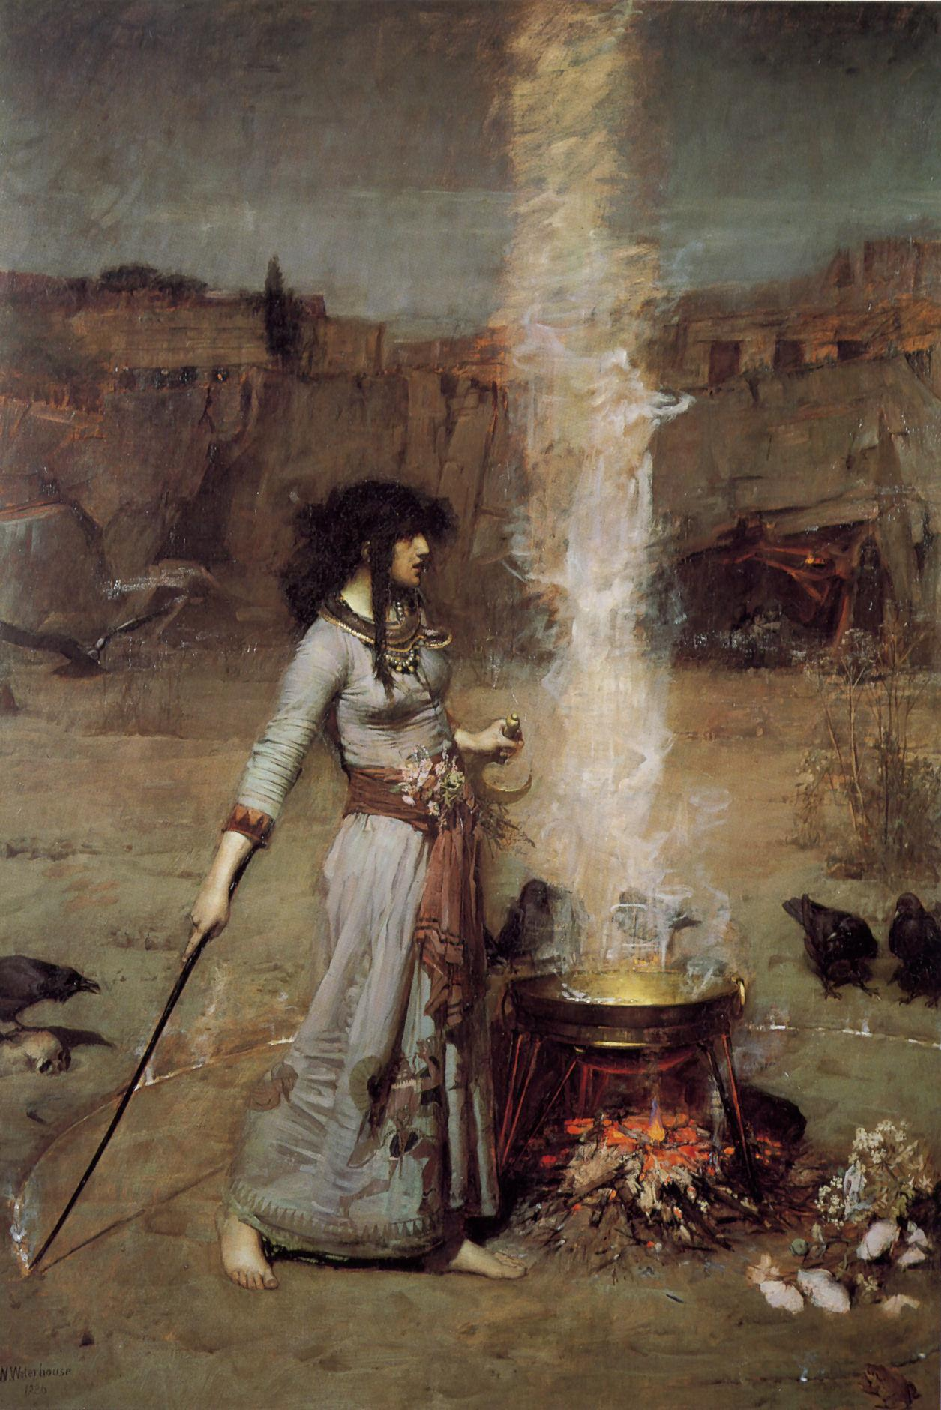
\includegraphics[width=0.80\textwidth]{graphics/frontmatter/j_m_waterhouse_magic_circle.pdf}

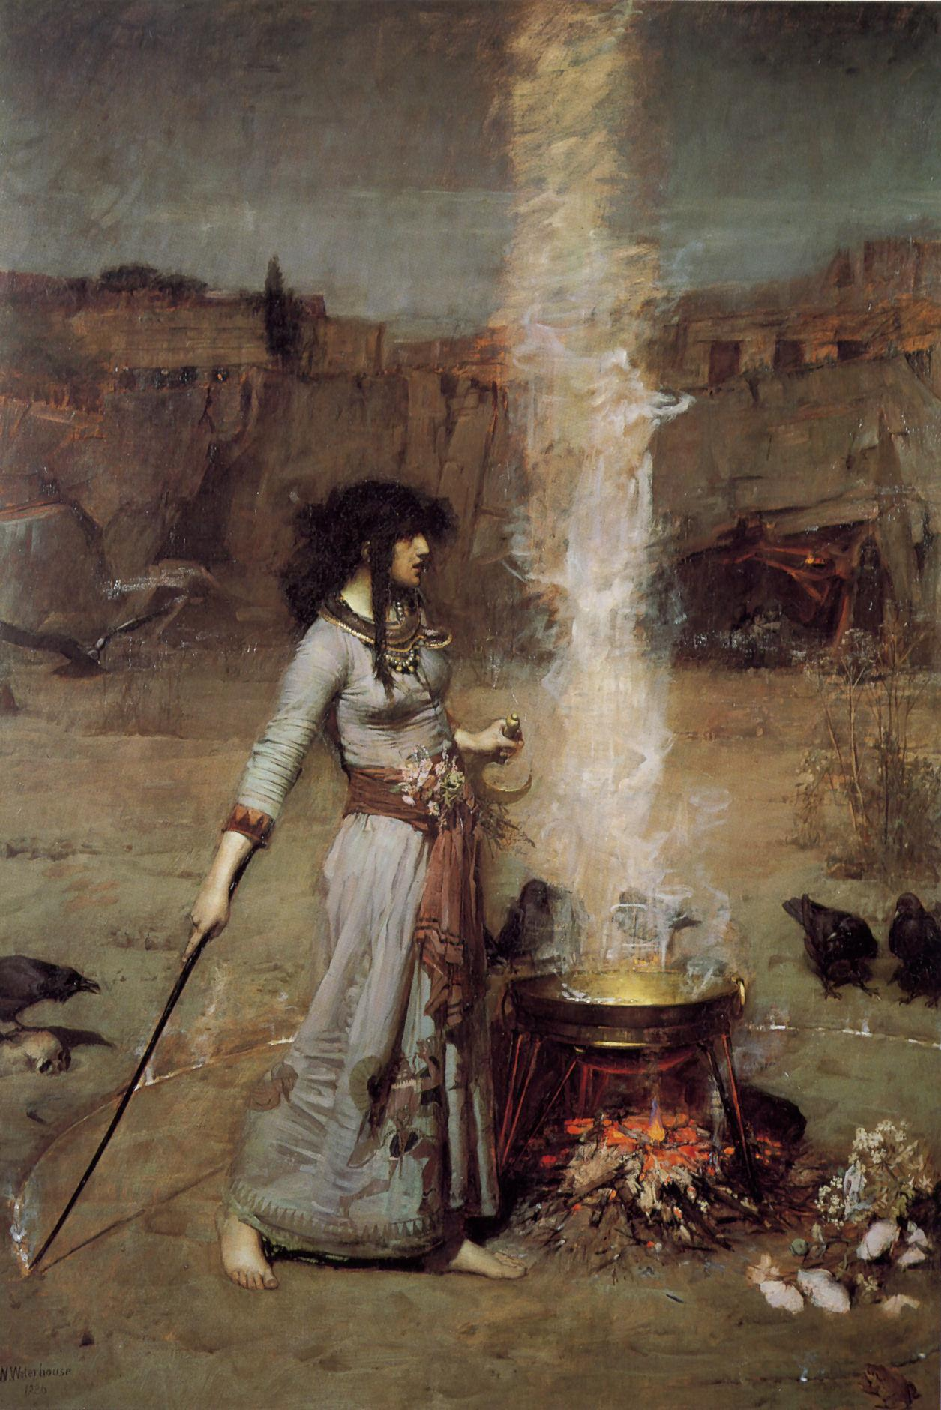
\includegraphics[width=\textwidth]{graphics/frontmatter/j_m_waterhouse_magic_circle.pdf}
\caption*{\emph{The Magic Circle by J. M. Waterhouse}}
\end{figure}
\restoregeometry
%TITLE PAGE
\phantomsection
\addcontentsline{toc}{chapter}{Title}
{
\Huge\bfseries\centering\headingfont The Statistical Grimoire: \\
Statistics for the Natural Sciences Using R\\

\vspace{0.5em}

\small\mdseries\raggedright Version 1.0.5

\rule{\linewidth}{1pt}\\[-6mm]
\rule{\linewidth}{2pt}\\

}

\vskip 2cm

\begin{center}
\Large Dr. Jeffrey M. Pisklak \\
\vspace{0.5em}
\large University of Alberta
\end{center}

\vfill

%https://stackoverflow.com/questions/615227/how-to-do-version-numbers
%[complete-ish chapter].[substantial edits].[minor edits]
\vspace*{\fill}

%\begin{wrapfigure}[3]{r}{0.15\textwidth}
\setlength{\intextsep}{1pt}%
\setlength{\columnsep}{8pt}%
\begin{wrapfigure}{r}{0.2\textwidth}
\href{https://creativecommons.org/licenses/by-nc-nd/4.0/}{\includesvg[scale = .6]{graphics/frontmatter/by-nc-nd.svg}}
\end{wrapfigure}

{
%raggedright
\noindent
The Statistical Grimoire: Statistics for the Natural Sciences Using R by \mbox{Jeffrey} M. Pisklak is licensed under \href{https://creativecommons.org/licenses/by-nc-nd/4.0/}{Creative Commons Attribution-NonCommercial-NoDerivatives 4.0 International}.

\noindent
%\pdftexbanner \\
\luatexbanner \\
Generation Date: \today{}



\noindent
\faIcon{globe} \url{https://statistical-grimoire.neocities.org/} \\
\faIcon{github} \url{https://github.com/statistical-grimoire/book} \\
\faIcon{envelope} statistical-grimoire@proton.me


\noindent
Frontispiece image: Waterhouse, J. M. (1886). \textit{The Magic Circle} [Painting]. The Tate Gallery - London, England
}


% https://creativecommons.org/
%%Dedication
\null\vfill

\begingroup\centering

{\large \itshape
This book is dedicated to the only three good math instructors I ever had. It is written in spite of all the others.
}

\endgroup

\vfill

\cleardoublepage

\pagestyle{plain}
\onehalfspacing
%Preface
\chapter*{Preface}
\addcontentsline{toc}{chapter}{Preface}
Since prefaces often go unread, I shall keep this brief. This text was born out of a need to offer my students a robust, open-access (i.e., free) introduction to R, specifically for those without any programming experience. Long term it is intended to serve as a practical, open-access manual, guiding complete beginners through both statistics and statistical programming in a thorough and clear manner. Please consider everything herein a work in progress.

\vspace{2em}

{
\headingfont \Large
\noindent Foolish Assumptions Made by Your Author:
\normalsize\normalfont
\begin{itemize}
    \item Students will read this (yes, I'm an optimist).
    \item The reader probably hates math, but realizes that math is like physical exercise - necessary, but rarely enjoyable and often exhausting.
    \item Beginners with R and programming will start this book at the beginning and move sequentially through the topics (because skipping ahead is like summoning a demon without comprehending what you are really doing. You’ll regret it. Of that I am confident.).
    \item Readers will not take the sillier things I say in this book too seriously.
\end{itemize}
}

\vspace{2em}

{
\headingfont \Large
\noindent Errata:
\normalsize\normalfont
\begin{itemize}
\item No manuscript, however cursed or consecrated, is free from the creeping taint of error. Should you unearth any faults, oversights, contradictions, or anomalies—do not consign your discovery to silence. Instead, record your findings within the digital vaults of GitHub, where the keeper of this tome may attempt to contain and exorcise the corruption...before it spreads further.
    \begin{itemize}
        \item \url{https://github.com/statistical-grimoire/book/issues}
    \end{itemize}
\end{itemize}
}



\tableofcontents

%----------------------------------------------------------------------------
% MAINMATTER: the main content of the textbook
%----------------------------------------------------------------------------
\mainmatter
\pagestyle{fancy}
\onehalfspacing

\part{R Programming - An Initiation}

\IMFellEnglish

What lies ahead in this first part is nothing short of a trial by fire. This section contains a wealth of information that, at first glance, should feel overwhelming - like staring into the heart of an inferno. Any reader who believes this content must be memorized is venturing down a perilous path, one that will surely lead to being consumed by the flames they are stepping in to.

The goal here is not to transform the reader into an expert with R, programming, or statistics. Instead, this section is designed to immerse the reader in the R language, offering hands-on experience while building a strong foundational understanding. Think of it as the first incantations in the dark art of programming. The focus should be on grasping the underlying logic of the code rather than committing it to memory.\footnote{Every section in this book has a corresponding bookmark in the PDF file for quick reference.} Programming is not merely a list of spells to recite by rote—it is a craft, a skill honed through practice and understanding. Readers would do well to approach it wisely, or risk being scorched by the fire they seek to wield.

\chapter{An Introduction to R}

To begin with ...

\section[What the f**k is R?]{What the f**k is R?\footnote{If you are wondering why the harsh language, it's because I get it, at face value, learning a programming language to do stats seems really f**kin' stupid. But if you can temporarily hold back your gag reflex, I will try my best to convince you otherwise.}}

\lettrine{R}{ } is a \gls{programming language}. A programming language is simply a language humans use to give instructions to computers. Humans are of course featherless bipedal primates called \textit{Homo sapiens}. Computers are machines that follow fixed rules, with no authority to deviate from those rules \parencite{Turing1950}. Contrary to the belief of many, what constitutes a human and what constitutes a computer are not mutually exclusive. In the past, computation was a biological endeavor, with humans relying on other humans to carry out the laborious task of performing countless mathematical calculations. These human computers required no strict programming language, \textit{per se}, but instead relied on the grunts and scribbles of primates in the upper tiers of their hierarchy to dictate their tasks.  In the modern day, human computers are largely a relic of the past, a product of a bygone era where mathematics and other concepts foreign to modern students, such as reading and writing, were commonplace within school curricula. 

Today the electronic digital computer reigns supreme.  This is a machine, largely silicon based, and similar in many respects to its primate precursor - with the notable exception that it is considerably more logical (some even go so far as to call these devices ``smart'' - which perhaps says more about the users than the devices themselves). It is therefore no longer deemed necessary to subject children to the cruelties associated with a well rounded education, particularly in the domain of mathematics, where the largest amounts of physical and psychological turmoil were often inflicted.

\subsection{The Genesis of R}

The name ``R'' was derived from the first initials of its original two programmers, \textbf{R}obert Gentleman and \textbf{R}oss Ihaka.  The decision to name the language using a single English letter is what we might, charitably, call a joke on the part of these two programmers, who saw themselves poking fun at R's parent language, which was given the unimaginative name of ``S''. In the 1970s the S language had undergone its initial development at the famous Bell Laboratories with the primary aim of enabling and encouraging ``GOOD DATA ANALYSIS''- a goal so fundamental to the ethos of S that the authors, \textcite{Becker1984}, felt they had to emphasize it using uppercase lettering inside the preface to the language's inaugural instruction manual (the uppercase lettering has been reproduced here for the reader's benefit). The familial correspondence R has with S is present even to this day, to such an extent that \textcite{Becker1984} original manual could probably function decently well as an introductory manual to R itself.

\section{Why the f**k should I use R?}

At this point readers might be wondering why it should ever be necessary to learn a programming language to conduct statistics and data analysis more generally. These topics are usually considered difficult enough by many students and educators, what need is there to compound this with a programming language? Why not, for instance, make use of any one of the many pieces of statistical software that already exist and require no requisite knowledge of any kind of programming? In other words, why not use software such as SPSS?\footnote{SPSS is popular software for conducting statistics that was originally released in the late 1960s and is an acronym for \textit{Statistical Package for the Social Sciences}. At some point it was purchased by IBM and re-branded to mean \textit{Steeply Priced Shitty Software.}}

The principal answer to this question has to do with flexibility. It is not the case that there is always a single correct way to do things.  Different sets of data come with their own unique intricacies and problems which are often not amenable to the ``cookie cutter'' style of analyses the aforementioned program employs. Which is not to say that a program like SPSS is incapable of adapting to these scenarios. It usually is, but this adaptation either requires the user to pay for some additional feature they did not get in their original purchase or it demands a much higher level of expertise with the software than most users are ever likely to acquire - expecting them to learn some obscure programming language, specific to that software, that all but a privileged few actually comprehend. Along these lines, something that non-R users often do not appreciate is how easy R is to learn. At a superficial glance, R can appear intimidating but it is actually fairly intuitive and works, more or less, in the manner of a calculator.  Most people who learn R find it to be a rewarding experience that was considerably more user friendly than what its paid counterparts produced \parencite{Bro}. This is thanks in large part to the extensive infrastructure of helpful online resources R users have built over the years - which proprietary equivalents have no equal to. Software like SPSS can give an air of familiarity when a user first encounters them because, superficially, they appear very similar to commonly used spreadsheet software many individuals will already be acquainted with, such as Microsoft's Excel. The user is typically provided with a hefty amount of buttons and menus at the top of the screen followed by a spreadsheet-style grid beneath it. Unfortunately, that is where the similarities end and new users inevitably find themselves overwhelmed by the plethora of bewildering options to perform what should be simple enough tasks (e.g., loading and viewing a data set). The dirty little secret about these programs is that their learning-curve is considerably steeper than their advertising would have you believe.  By contrast there is an inherent logic to R (the logic of mathematics) that new users can often easily grasp and build off of (even if you don't like math). Moreover, R is not beholden to a graphical user interface (i.e., a gui - pronounced ``gooey'' and often referred to as a ``point and click interface.''). Consequently, its functionality is only limited by what you, or other people, are able to program and what your computer is capable of handling.

%%% https://www.fogcam.org/

An altogether different answer to the question that opened this section, and one that will appeal to the University students reading this, is simply cost. R is free for the user, with no need to put up with annoying advertising or pay for additional features. The same can not be said of the other aforementioned software which are almost always subscription based, requiring the user to consistently renew an expensive license to use the software. In fact, upon visiting the respective websites for both SPSS and another, slightly less well known, SPSS style software called Minitab, one can see that it is worryingly difficult to find any price listings whatsoever for these programs - evoking the age old wisdom that, if you have to ask the price, you probably can't afford it.  But R is not just free in monetary terms, it is also free in philosophical terms. R adopts the Free Software Foundation’s GNU General Public License and thus adheres to the philosophy of ``free software'' (what some might term ``open-source'').  From the GNU project website \parencite{GNUphil}:

%\sffamily
{
%\fontfamily{artemisia}\selectfont
\begin{displayquote}
\headingfont
A program is free software if the program's users have the four essential freedoms:

\begin{itemize}
\item Freedom 0: The freedom to run the program as you wish, for any purpose.
\item Freedom 1: The freedom to study how the program works, and change it so it does your computing as you wish. Access to the source code is a precondition for this.
\item Freedom 2: The freedom to redistribute copies so you can help others.
\item Freedom 3: The freedom to distribute copies of your modified versions to others. By doing this you can give the whole community a chance to benefit from your changes. Access to the source code is a precondition for this.
\end{itemize}
\end{displayquote}
}
%\rmfamily

This philosophy applies not only to the software itself but also to its various file types and help documentation. For many years, a significant barrier to the dissemination of scientific findings has been the reliance on exclusive file formats by proprietary research tools. Clearly, locking information in this manner is not in the best interest of scientific progress; rather, it serves to tether researchers to an overpriced, branded ecosystem. Consequently, we can rightly label the continued adoption of these practices as unscrupulous. In practical terms, what this means is that, if for no other reason, we should use R just to give the middle finger to these companies.

%For instance, many types of paid software used for building, running, and analyzing computer-based experiments will, by default, output results using restrictive file formats that require the original software with a valid license to be read. This not only makes it difficult to provide free access of the data to other researchers, but makes it that much more difficult to load the data into other types of software (which are also likely to contain their own proprietary formatting schemes) for more in-depth analyses than what the original program affords the researcher.  Obviously, in a by-gone pre-internet era, when statistical computing was both a complex and expensive endeavour, and the use of any given computer and its software was restricted to a small coterie of researchers, a company may be forgiven for utilizing proprietary formatting schemes in this manner.  However, in an age where the internet is ubiquitous and there is rarely any need to ration computing power, there is little justification for such practices. A generic .CSV (comma-separated values)\footnote{A ``comma-separated values'' spreadsheet is a universal file format for spreadsheets. It is readable by any competent spreadsheet software and, in fact, spreadsheet software is not even necessary to read a .CSV file - a basic text editor will suffice. Moreover, .CSV files can contain large amounts of information with comparatively small file sizes.} spreadsheet file will be sufficient as an output for most research endeavors. It is clear to any reasonable person that locking information away in this manner is not done in the best interest of scientific progress; rather, it is done simply to tether researchers to a branded ecosystem of overpriced software. Consequently, we can easily label the continued adoption of these practices for what they are: unscrupulous. In practical terms, what this means is that, if for no other reason, we should use R just to give the middle finger to these companies.

\section{Installing and Running R on Your Computer}

\subsection{Languages and Environments}
\label{sec:LangAndEnv}

R will install and run straightforwardly on Windows and Macintosh operating systems as well as Linux; however, prior to attempting any install it is important to make a simple distinction first.  R is a programming language, which means it is nothing more than a language you can use to communicate instructions to your computer. To communicate those instructions, some type of interface is required.  This is a basic reality that applies to any language.  It is quite difficult to communicate with someone if they have no mouth, eyes, or ears to send and receive communications with. Computers are no different in this respect. Simply ``understanding'' the language is not sufficient.  For this reason, most operating systems come equipped with a basic way of interfacing with the user via a \gls{command console}\footnote{A windowed application that allows you to type instructions (a.k.a. ``commands'') to your computer.} of some kind. On computers using the Windows operating system, this is referred to as the \textit{Command Prompt} application, on Macintosh computers this is the \textit{Terminal} application. Relying on your operating system's basic command console as a primary interface is often a cumbersome and inefficient experience, and definitely not a recommended course of action - though, for what it is worth, Linux users seem to delight in this sort of thing. The preferred means of communicating R to your computer is via the use of what, in programming lingo, is commonly termed an ``\textbf{environment}'' or, more garrulously, an ``\gls{integrated development environment} (\acrshort{IDE})''.  This is simply a software application providing the user with a more elegant visual workspace and feature set to make programming a smoother experience. 

The standard installation of R will come with an associated environment for the user - provided they are working with either a Windows or Mackintosh operating system.  However, while this environment is preferable to the operating system's basic command console, most R users still find it lacking and opt to install a different environment called \href{https://posit.co/}{\gls{RStudio}}, which has an open-source (free) version for non-commercial use.

\subsection{Installation}
\label{sec:install}

To install R - both the language and the environment simultaneously - simply go to the \textit{R Project for Statistical Computing} website: 

\begin{center}
\url{https://www.r-project.org/}
\end{center}

\noindent
Somewhere on the front-page of this website should be a link labelled ``\acrshort{CRAN}''. This stands for \gls{Comprehensive R Archive Network} and is a set of servers around the world that distribute R alongside packages associated with R.  The servers are ``mirrored'', meaning they all provide the same content.  So there is no need to worry about one server providing incomplete, out-of-date, or unofficial versions of R.  Technically speaking, the server closest to your home location is the one you should opt to download from; however, the topmost link labeled ``0-Cloud'' will be sufficient for most users.  The install file is only about 80 megabytes large, so unless you live in the remotest areas of Earth, download speed, and thus choice of server, is probably not a concern.

Once you have chosen a suitable server, you will need select your operating system and choose the appropriate installation file. If you are using Windows, opt to download the ``base'' version of R.  If you are using a Macintosh operating system, you will need to select the option relevant to your computer.  At the time of writing this, Macintosh computers have recently begun being manufactured using their own in-house built processors (i.e., dubbed ``Apple silicon''); however, many older Macintosh computers (pre-2023) still contain Intel-made processors. The install file you select will need to be determined by which type of processor your computer is using. Macintosh users can determine this by selecting \textit{About This Mac} via the small little apple logo in the top left corner of the desktop screen. Machines using Apple silicon, will display a row called ``Chip'' and state something akin to ``Apple M1''. Machines using Intel processors will display a row reading ``Processor'' followed by the make and model of the processor.

Downloading and running the install file should prompt you with a installation wizard that walks you through the installation process. Unless you are certain you know what you are doing (which means you probably aren't reading this), you should just accept the wizard's default settings.

Upon installation of R, you can then install the aforementioned RStudio environment at

\begin{center}
\url{https://posit.co/products/open-source/rstudio/}
\end{center}

Installing RStudio is not strictly necessary to work through this book's content; however, the wealth of features and customization RStudio offers does makes it a worthwhile program to install and is recommended for anyone reading this text.

\subsection{Upgrading}

There are updates made to R about 2-3 times a year and it is generally good practice to upgrade regularly. There are various methods you can use to update R, but the most straightforward method is to just download the latest version of R as though you were installing it for the first time and then re-install commonly used packages.\footnote{Packages (also called ``libraries'') will be explained later.} If you follow the default setup, you do not need to uninstall the previous version. In fact, it is usually preferable not to, as RStudio allows you to easily switch between installed versions on your computer.

At the time of writing, R is on version 4.4.1, nicknamed the ``Race for Your Life'' version.  New releases of R are given nicknames that, inexplicably, are all obscure references to Peanuts (a.k.a. Charlie Brown and Snoopy) comic strips.

\subsection{Consoles and Scripts}

Upon opening the base R environment you will be shown a pane labelled \textit{R Console}.  Opening RStudio environment will show a similar pane simply labelled \textit{Console} alongside a couple of others.  The console pane functions as the command console described earlier (see section \ref{sec:LangAndEnv}).  Inside it you will see a ``$>$''. This symbol denotes the command line's prompt.  In other words, it denotes the space in which you type commands, using R code, to your computer.  The term ``code'' here is just a shorthand way of referring to ``computer code'' which is another way of expressing the fact that we are typing commands using a programming language. The presence of $>$ also indicates that the computer is awaiting your command.

If you type $1 + 1$ on this line and the press ``enter/return'' on your keyboard, you should see a 2 display as an output almost instantaneously beneath it.  In this case the expression ``$1 + 1$'' is a \textit{line of R code}.  Pressing enter/return, \textit{runs} or \textit{executes} this R code. And ``$2$'' is the computer's resulting \textit{output}.

\textbf{Input:}
\begin{inR}
1 + 1
\end{inR}

\vspace{1em}

\textbf{Output:}
\begin{outR}
[1] 2
\end{outR}


If you close R or RStudio, you will find that any history of this calculation is gone when you re-open the environment.  Consequently, typing commands into the console offers us a quick way to perform simple tasks that we are not necessarily concerned with preserving.  However, in most cases we will be typing R code that we do want to preserve, run, edit, and add to at later date.  This is where the concept of a \gls{script} becomes important.

A script is simply a text document on your computer that you can use to type, run, edit, and save your R code. Using the base R environment, selecting the \textit{File} menu at the top left corner and choosing \textit{New Script}, will open a scripting window.  In R Studio the process is \textit{File $\rightarrow$ New File $\rightarrow$ R Script}.  

Once opened, you can type R code into this new window and save it in the conventional manner of most word processing applications (i.e., \textit{File $\rightarrow$ Save As}). For instance, if you type the following into the script window ...

\begin{inR}
1 + 1
2 + 2
3 + 3
\end{inR}

\medskip

You can now place your cursor at a line of your choosing and run that line individually.  To do this in the base R environment you select \textit{Edit $\rightarrow$ Run Line or Selection}.  In RStudio you select \textit{Code $\rightarrow$ Run Selected Line(s)} or click the ``run'' icon in the upper right of the script window. If you highlight all the lines of code, or just a subset of them, you can then run that highlighted section in a similar manner.

\subsection{Keyboard Shortcuts}
\label{sec:key_short}

It is at this juncture that a handy feature of programming environments be mentioned; specifically, keyboard shortcuts (also called ``hotkeys''). All good programming environments will provide their users with the ability to do every conceivable task via their keyboard in some way. For instance, if you are using the Windows operating system, pressing the ``control'' key simultaneously with the ``s'' key will save your script file (Ctrl + S). Learning the shortcuts for frequently used features, such as selecting and running lines of code, can make the process of writing code considerably more time efficient and effortless.  In theory, a good programmer - using a competently developed coding environment - should never require the use of a mouse.  RStudio, in particular, offers a wide range of keyboard shortcuts that can be customized to user preferences.  For instance, selecting \textit{Help $\rightarrow$ Keyboard Shortcuts Help} will display a list of existing shortcuts that users can avail themselves of.  Please note, it is not being suggested that you go out of your way to memorize all of these at once. The simple act of trying to use them consistently will be sufficient to learn them in an effortless manner. At the outset, it is to your advantage to merely select a few and attempt to use them consistently while you code. A few of the most useful ones are listed in Table \ref{table:keyShorts}\footnote{Shortcuts 3, 4, and 5 can be combined with shortcut 6 to highlight bigger sections of code.}.

\vspace{1em}

\begin{table}[h]
\centering
\resizebox{\textwidth}{!}{%
\begin{tabular}{@{}llll@{}}
\toprule
 & \textbf{Description} & \textbf{Windows} & \textbf{Macintosh} \\ \midrule
1. & Run current line/section & Ctrl + Enter & Cmd + Return \\
2. & Clear Console & Ctrl + L & Ctrl + L \\
3. & Move to the beginning of a line & Home & Cmd + Left \\
4. & Move to the end of a line & End & Cmd + Right \\
5. & Move the cursor one word/block at a time & Ctrl + Left or Right & Option + Left or Right \\
6. & Highlight all & Ctrl + A & Cmd + A \\
7. & Highlight sections & Shift + Up, Down, Left, or Right & Shift + Up, Down, Left, or Right \\
8. & Move cursor to script window & Ctrl + 1 & Ctrl + 1 \\
9. & Move cursor to console window & Ctrl + 2 & Ctrl + 2 \\
10. & Type the \R{<-} operator & Alt + - (minus) & Option + - (minus) \\ \bottomrule
\end{tabular}}
\caption{Useful Keyboard Shortcuts}
\label{table:keyShorts}
\end{table}

\begin{figure*}[!b]
    \centering
\begin{mdframed}[style = miscFrame, frametitle = Box 1.1: Are you using your keyboard properly?]

When utilizing the keyboard shortcuts mentioned in section \ref{sec:key_short}, it is worth remembering that standard QWERTY-style keyboards are symmetrically designed. Modifier keys like the \textit{shift} key, \textit{control} key, and \textit{alt} key are located on both the left and right side of the board.  This is not by accident and many people - even those who have grown up with unprecedented access to computers and the internet - have never learned to appreciate the utility of this layout or use it appropriately. \\

As an example, to type capital letters you should always depress the shift key on the opposite side of the keyboard to the letter. So, if you desired to type the capital letter Q, you would depress the right shift key with your right hand, and type Q with your left hand.  A similar logic applies to the other modifier keys. To use keyboard shortcut \#9 in Table \ref{table:keyShorts}, you would depress the right control key (with your right hand) and use your left hand to press the 2 key.  You should not be trying to press both keys with a single hand.  Such advice might seem obvious but, given the sheer number of people who contort their wrists and fingers in grotesquely strange and painful ways, it is clearly far from being so.

\end{mdframed}
\end{figure*}


\section{How To Code Using R: The Fundamentals}

With the formalities of installation, console, and scripting window out of the way, we can now start to learn how to write (i.e. code) using the language called R.  Though, it is at this juncture that some advice to novice programmers be offered.  Nothing that will be discussed in this section, or any section of this text concerning R code, is material you need to go out of your way to memorize.  R is a language, and the basic act of trying to use the language consistently will result in a natural and effortless memorization over time. Along these lines, there are some basic recommendations novice programmers can follow to expedite this:

\begin{itemize}
    \item Do not use your computer's copy and paste functions.  Type all code yourself.
    \item Run all the examples in this textbook and try and produce the same results.
    \item If you do not know how to do some particular thing, then look up how to do it each time you need to do it.
    \item Stay organized - this applies to the code you write and the files you save.
    \item Pledge to do all your stats from this point forward using R. Immerse yourself in the language.
\end{itemize}

\noindent
Everything discussed here is done so for the purpose of acquainting you with the R language so that, when you see some R code, you are not compelled into some manner of zombiesque torpor.  As you move through the text, you will learn more advanced things and have much of this material repeated and re-explained.  Your goal in this chapter is not to become an R expert, but rather to get an intuitive grasp of R's underlying syntax and logic.


\subsection{Basic Arithmetic}

At its core R is really nothing more than a fancy calculator, and we can use it as such.  R can be used to add ($+$), subtract ($-$), multiply ($\times$), and divide ($\div$).

\begin{inR}
1 + 1
2 - 2
3 * 3
4 / 4
\end{inR}

\begin{outR}
[1] 2
[1] 0
[1] 9
[1] 1
\end{outR}

Exponents can be incorporated as well by using the $^\wedge$ (`caret'), symbol. For instance, the expression $5^3$ can be written as ...

\begin{inR}
5^3
\end{inR}

\begin{outR}
[1] 125
\end{outR}

R will also follow the \textit{order of operations} when dealing with more complex expressions.  To illustrate, consider the mathematical expression $8\div2(2+2)$. Some people mistakenly believe that this expression is equal to $1$, some believe it is equal to $4$, and others believe that it is improperly written and there is no solution. In fact, it is equal to $16$. As many will no doubt have learned in their primary education, according to order of operations (BEDMAS\footnote{BEDMAS of course being the famous mnemonic to help memorize the order of operations: Brackets, Exponents, Division, Multiplication, Addition, and Subtraction. Many non-Canadian readers may be more familiar with an inferior variant of this mnemonic known as PEDMAS.}), the order in which you divide and multiply inside the equation is not fixed, sometimes you divide first and sometimes you multiply first. However, what most people never learn is that the order you use is not up to you. You must always calculate from left to right when making a choice between multiplication and division.  The same rule applies to addition and subtraction.

\begin{inR}
8/2*(2+2)
\end{inR}

\begin{outR}
[1] 16
\end{outR}

\noindent
If we re-write the equation to be $8\div(2+2)2$, you will see a corresponding change in the computer's output.

\begin{inR}
8/(2+2)*2
\end{inR}

\begin{outR}
[1] 4
\end{outR}

R also has the ability to perform \textit{Euclidean Division}, which many simply know from their primary education days as \textit{division with a remainder.}  For instance, consider $11 \div 2$.  Conventionally, you would want and expect an answer of $5.5$, and R will produce that.

\begin{inR}
11/2
\end{inR}

\begin{outR}
[1] 5.5
\end{outR}

\noindent However, if we want to see the result expressed as a quotient and remainder (i.e., if we want to use Euclidean Division), we could obtain the quotient by typing ...

\begin{inR}
11 %/% 2
\end{inR}

\begin{outR}
[1] 5
\end{outR}

To obtain the remainder we type...

\begin{inR}
11 %% 2
\end{inR}

\begin{outR}
[1] 1
\end{outR}

Thus, 11 can be split into 2 groups of 5, with 1 left over.  More technically, the \R{\%\%} is what is known as the \gls{modulo operator} and the remainder value of \R{1} that results from \R{11 \%\% 2} is known as the \gls{modulus}.

Other, more complex, arithmetic operations are available in the R language; however, most of them will require the use of specialized lines of code called \textit{functions}, which are discussed later (see section \ref{sec:functions}). 

Given that we are on the topic of basic arithmetic, it is perhaps worth considering what happens when you ``break the rules'' of basic arithmetic. Suppose we divide a positive and negative value by zero, what will happen?

\begin{inR}
1/0
-1/0
\end{inR}
\begin{outR}
[1] Inf
[1] -Inf
\end{outR}

\noindent
You can see that R produces a result of \R{Inf} and \R{-Inf} which is an abbreviated way of referring to \gls{infinity} in the positive and negative directions respectively.\footnote{This will also be generated if a number is too large for a computer to cope with. For example, the code \R{.Machine\$double.xmax} will produce the largest number your computer can handle. R will technically still let you \textit{add} values to this number, but the number won't change from R's perspective because the amount you would have to add to alter what is shown is excessively large. However, if you \textit{multiply} it by 2, you should get \R{Inf}: 
\R{.Machine\$double.xmax * 2}}.

What happens if you take the square root of a negative number? 

\begin{inR}
(-4)^(1/2)
\end{inR}
\begin{outR}
[1] NaN
\end{outR}

The abbreviation \R{NaN} here stands for ``not a number'', and is a fairly sensible output given that the square root of a negative number does not exist as a real number (consequently, it only exists in your imagination).

Finally, since its use crops up from time to time, it can be handy to know that R comes with the number $\pi$ stored as a constant. To use it, you need only type \R{pi}.\footnote{If you find $\pi$ displayed to seven digits inadequate, you may want to talk to a professionally licensed therapist. Alternatively, you can display more digits by running the code \R{print(pi, digits = 16)}. Values exceeding 16 digits will be inaccurate given the limitations of 64-bit computers, so it is advisable not to go beyond 16 even though a max of 22 are possible. If you want R to always display all 16 digits, you can change its default behaviour by running \R{options(digits = 16)}, though this is not recommended.}

\begin{inR}
pi
\end{inR}
\begin{outR}
[1] 3.141593
\end{outR}

\subsection{Understanding Scientific Notation}

On occasion values will be either excessively large or excessively small. In such cases R will often display the values using what is referred to as \gls{scientific notation}.  For instance, dividing the number $2$ by $100000$ will result in scientific notation being employed:

\begin{inR}
2 / 100000
\end{inR}
\begin{outR}
[1] 2e-05
\end{outR}

Notice the \R{e-05} in the output. This is how you know R is presenting a number using scientific notation. To interpret this in a conventional manner, imagine there is a decimal point after the 2, like so: \R{2.0e-05}. Then just move that decimal point five digits to the left. In other words, \R{2e-05} is the same as writing \R{0.00002}. Mathematically, \R{2e-05} translates to $2 \times 10^{-5}$

If the output were showing \R{e+5}, then you would move the decimal five digits to the right. For example, \R{2e+5} is the same as writing \R{200000}. Notice there are five 0s; this is because, mathematically, \R{1e+5} means $2 \times 10^5$

Remember that positive powers move the decimal right (in the positive direction), and negative powers move the decimal left (in the negative direction).


\subsection{Commenting Out Lines}
In the course of writing R code, there will be occasions where you would like to run a script you have typed up, but not necessarily run every single line on that script.  There might be certain lines that you would, at least tentatively, like to keep for one reason or another but not necessarily run.  You can accomplish this by ``commenting out'' your code.  If you type a \R{\#} symbol, any code that follows that symbol and is on the same line as that symbol will not be run.

\begin{inR}
1 + 1
# 2 + 2
3 + 3
\end{inR}
\begin{outR}
[1] 2
[1] 6
\end{outR}

\begin{inR}
1 + 2 + 3 # + 4 + 5
\end{inR}
\begin{outR}
[1] 6
\end{outR}

\noindent
This process is phrased ``commenting out'' because using the \R{\#} is also frequently employed to write \textit{short} helpful comments to yourself and other readers about your R script.


\subsection{Creating Objects}

A central feature of R is its ability to call objects in memory. For instance, we can define an object name, \R{x}, and have that name represent a number by typing a little arrow, \R{<-}, and following it with a value such as 1.

\begin{inR}
x <- 1
\end{inR}

\vspace{1em}

You will find that running this line of code produces no corresponding output.  However, if we now run \R{x} by itself the computer will display an output of $1$

\begin{inR}
x
\end{inR}

\begin{outR}
[1] 1
\end{outR}

R is technically classified as an object-oriented programming language (an ``OOP''). This is because, if you look into how R actually stores what we have done in memory, the ``object'' here is the number 1.  \R{x} is merely the name we are assigning to that object. However, a lot of R users are under the impression that the reverse is true - i.e., that we have in some sense created an object called \R{x} and stored something inside of it, but that is not actually the case. \R{x} is just a name binded to the object 1, and this object 1 is located somewhere inside your computer's memory. Admittedly, unless you are doing some seriously advanced R programming, this is a distinction that will not matter to 99.3\% of R users, but it is important because it means that if you do something like this . . . 

\begin{inR}
x <- 1
y <- 1
\end{inR}

\vspace{1em}

\noindent \R{x} and \R{y} are technically different objects in the computer's memory.  However, if we did this ....

\begin{inR}
y <- x
\end{inR}

\vspace{1em}

\noindent they now represent the same object in memory. Moreover, altering one does not affect the other and just ends up creating two separate objects in memory. E.g. ...

\begin{inR}
x <- x + 1
x
y
\end{inR}

\begin{outR}
[1] 2
[1] 1
\end{outR}

To assign the names \R{x} and \R{y} we typed an arrow, \R{<-}. Alternatively, we could have assigned the names using an equal sign (\R{=}) instead.

\begin{inR}
y = x + 4
y
\end{inR}

\begin{outR}
[1] 6
\end{outR}

Both \R{<-} and \R{=}, in the manner we are using them here, are what are referred to as \glspl{assignment operator} in that, they are used to perform the \textit{operation} of \textit{assigning} a name to an object. For most use cases, there is no practical difference between the two; except insofar as the arrow can be swapped around to assign values to objects like so.

\begin{inR}
10 -> z
z
\end{inR}

\begin{outR}
[1] 10
\end{outR}

The existence of both \R{=} and \R{<-} as assignment operators raises an obvious question: which is better to use?  This is a question for which there are strong opinions and Appendix \ref{sec:AppendixOperator} walks through the trivial dispute for those interested.\footnote{TL;DR: While code written using \R{=} tends to have an intuitive appeal and requires one less key to press, the \R{<-} has greater functionality and is generally preferred by R's anointed high council (overseers of Tidyverse) for that reason. If you opt to use \R{<-}, it is worth noting that RStudio contains a keyboard shortcut that offers a more ergonomic means of typing \R{<-} by pressing the \textit{alt} key followed by a minus (-) sign.}

\subsubsection{Object Modes}
\label{sec:modes}

Thus far all of the objects we have created have been \gls{numeric} objects; though, we can avail ourselves of other types.  For instance, another common object is the \gls{character} object which gets defined using quotation marks on each end of the value.

\begin{inR}
x <- "SPAM"
x
\end{inR}

\begin{outR}
[1] "SPAM"
\end{outR}

\noindent
Both single or double quotation marks can be used to define a character object. For instance, running ...

\begin{inR}
y <- 'SPAM'
y
\end{inR}

\begin{outR}
[1] "SPAM"
\end{outR}

\noindent
works just fine, but if you were to mix and match the two types of quotation marks (e.g., try to run \R{y <- "SPAM'}), you will find that no actual output is produced, and the console just displays the code you tried to run with a small \R{+} appended to it. The \R{+} indicates that the line of code is incomplete and more is expected before an output can be returned. If this happens you need only press the escape key (\textit{esc}) with your cursor inside the console window.

A key consideration about character objects, which will probably seem obvious, is that you cannot perform standard mathematical operations on them.

\begin{inR}
y * 5
\end{inR}

\begin{outR}
Error in y * 5 : non-numeric argument to binary operator
\end{outR}

\begin{inR}
2 + "2"
\end{inR}

\begin{outR}
Error in 2 + '2' : non-numeric argument to binary operator
\end{outR}

Another type of object is what is known as a \gls{logical} object.  This is an object that contains a value of \R{TRUE} or \R{FALSE} and is often referred to as a \gls{boolean} object.

\begin{inR}
x <- TRUE
y <- FALSE
x
y
\end{inR}

\begin{outR}
[1] TRUE
[1] FALSE
\end{outR}

The values \R{TRUE} and \R{FALSE} must be typed completely in uppercase without quotations for R to recognize them as a logical object.  Alternatively, R does permit a shorthand version of each.  Instead of typing \R{TRUE} and \R{FALSE}, you can type \R{T} and \R{F} respectively.  Though, for ease of reading, using this shorthand version is not advised.

Thus far, we have demonstrated three basic categories of object: \textit{numeric}, \textit{character}, and \textit{logical}.  R refers to these various categories as \textbf{modes}\footnote{You may sometimes hear these referred to as object ``classes'' as well. The distinction between modes and classes in R is nuanced, with considerable overlap between the two terms, though they are not perfectly equivalent. I have chosen to refer to object modes because it more consistently categorizes objects as numeric, character, or logical, which I believe is helpful for beginners learning R.}, and as you progress with R, both in this book and more generally, you will encounter other object modes. 

\subsubsection{Naming Objects}
\label{sec:namingObjects}

Oftentimes we will run into circumstances where other people are required to read, run, and modify the code we write.  Still other times, we may need to look at, and make sense of, code we have written in the past and largely forgotten. These considerations make it of the utmost importance that all of the code we write is intelligible to other people and our future selves. Among the best way to achieve this is by naming objects appropriately. Ideally, the name of an object should be concise and descriptive. Generally, you can name objects almost anything you like, as long as the name begins with a letter, contains no spaces, avoids special characters (except underscores \R{\_}), and does not use any of R's \gls{reserved words} such as \R{TRUE}, \R{Inf}, \R{NaN}, \R{function}, etc.

Given that spaces are not permitted in the naming of objects, programmers have developed certain conventions to promote readability. One such convention is \textit{snake case}, which separates lowercase lettered words with an underscore:

\begin{inR}
snake_case <- 1
\end{inR}
\medskip

\noindent
Another, referred to as \textit{camel case}, denotes separate words by capitalizing the first letter of each new word:

\begin{inR}
camelCase <- 2
\end{inR}
\medskip

\noindent
There is also \textit{period case}:
\begin{inR}
period.case <- 3
\end{inR}
\medskip

\noindent
There is \textit{random case} \parencite{Wickham2023}:
\begin{inR}
Ra.nD0M_CAs.e <- 4
\end{inR}
\medskip

\noindent
Finally, there is of course \textit{angry case} for those moments when you need to communicate your frustration with coding:
\begin{inR}
ANGRYCASE <- 5
\end{inR}
\medskip

Apart from the last two, R programmers tend to use all of these with seeming abandon. It is worth noting that different style guides for R have been developed and altered over the years with varying degrees of adoption. Presently there is no consensus on which style-guide should act in an official capacity for R; however, the most popular, and widely respected, is the Tidyverse Style Guide\footnote{The \textit{tidyverse} will be explained in the next chapter, just know that all the code written in this book will (do its best) to adhere to its standards.} (\url{https://style.tidyverse.org}) which advocates the strict and concise use of \textit{snake\_case} only.

When it comes to naming objects, all of the rules just laid out only apply to what are referred to as \glspl{syntactic name}; however, if you choose to be a psychopath, you can ignore all of those rules and create what are called \glspl{non-syntactic name} by simply enclosing the name within backticks.

\begin{inR}
`420 * 69` <- "PARTY TIME!"
`The devil made me do it!` <- "Hail Satan"
\end{inR}

\subsection{Vectors}

It is not the case that an object need store only a single value, as we have been doing above. Particularly when conducting statistical analyses, you are almost always working with variables that contain more than one value (i.e. multiple observations). In view of this, R objects can store as many values as you require.\footnote{Obviously, this statement is only true given the memory limitations of your computer's hardware and software.} For instance, if we want \R{x} to be equal to the numbers 1 through 5, we need only type: 

\begin{inR}
x <- c(1, 2, 3, 4, 5)
x
\end{inR}

\begin{outR}
[1] 1 2 3 4 5
\end{outR}

The lower case \R{c} is short for \textit{combine}. By combining the numbers 1 through 5 in this way we have created what is technically known as a \gls{vector}.\footnote{More specifically, we are speaking of \textit{atomic vectors} here, though most people just call them \textit{vectors.}} We can further use this combine function, \R{c()}, to combine vectors with other vectors. In the example below, we create two vectors, \R{x} and \R{y}, and combine them to create an object called \R{z}.

\begin{inR}
x <- c(1, 2, 3, 4, 5)
y <- c(6, 7, 8, 9, 10)
z <- c(x, y)
z
\end{inR}
\begin{outR}
[1]  1  2  3  4  5  6  7  8  9 10
\end{outR}

\begin{figure*}[!b]
    \centering
\begin{mdframed}[style = miscFrame, frametitle = Box 1.2: How to Use Your Colon Effectively \R{:}]

In the previous examples, we used R's combine function to create a basic set of ascending numbers. The need to generate regular sequences of integers is a common occurrence in data analyses, so R provides users with a convenient means to create them using the \gls{colon operator} (\R{:}).

\begin{inR}
x <- 1:5
x
\end{inR}
\vspace{1cm}
\begin{outR}
[1] 1 2 3 4 5
\end{outR} 

\vspace{\baselineskip}

This can also be used in reverse and with negative values.

\begin{inR}
3 : -5
\end{inR}
\vspace{1cm}
\begin{outR}
[1] 3  2  1  0 -1 -2 -3 -4 -5
\end{outR}

\end{mdframed}
\end{figure*}

The concept of a vector is one which will have relevance to people with a fondness of linear and matrix algebra\footnote{While I assume such people must exist, their existence is about as well-confirmed as that of the Sasquatch.} since it amounts to little more than a one-dimensional array/matrix. We can see how R handles vectors for these purposes by simply performing some mathematical operations on them.  For instance, if we add a single number to our vector, we can see that R straightforwardly adds that number to each element (i.e. position) in the vector.

\begin{inR}
x + 2
\end{inR}

\begin{outR}
[1] 3 4 5 6 7
\end{outR}

\noindent
Correspondingly:

\begin{inR}
x - 2
x * 2
x / 2
x^2
\end{inR}

\begin{outR}
[1] -1  0  1  2  3
[1]  2  4  6  8 10
[1] 0.5 1.0 1.5 2.0 2.5
[1]  1  4  9 16 25
\end{outR}

A similarly logical process is seen when we perform mathematical operations on two or more vectors of the same size.  For instance, adding them together results in the first element of one being added to the first element of the other.  The second element of one being added to the second element of the other, and so on.

\begin{inR}
x <- c(1,2,3,4,5)
y <- c(6,7,8,9,10)

x + y
\end{inR}

\begin{outR}
[1]  7  9 11 13 15
\end{outR}

\noindent
However, a curious thing will occur if the vectors have an unequal number of elements greater than 1. Suppose, as an example, one vector has four elements and another has five and we want to add them together. In the process of adding the first element with the first element, and the second element with the second, and so on, R will automatically loop back around to the first element in the shorter vector to complete the calculation; though, it does this only after giving you a warning.  Needless to say, you should not be performing any arithmetic on vectors of unequal lengths.

\begin{inR}
x <- c(1,2,3,4)
y <- c(6,7,8,9,10)

x + y
\end{inR}

\begin{outR}
Warning in x + y: longer object length is not a multiple
of shorter object length
[1]  7  9 11 13 11
\end{outR}

Vectors are also not limited to numbers. They can also contain character values and logical values.
\begin{inR}
a <- c(1,2,3)
b <- c("BREAD", "SPAM", "BREAD")
c <- c(TRUE, FALSE, FALSE)

a
b
c
\end{inR}

\begin{outR}
[1] 1 2 3
[1] "BREAD" "SPAM"  "BREAD"
[1]  TRUE FALSE FALSE
\end{outR}

\noindent
However, you cannot mix and match. For instance, if you have a character string amongst a set of numeric values, those numeric values will all be converted to character strings as evidenced by the quotation marks in the output.\footnote{You can also check the vector's mode by running \R{mode(d)}}

\begin{inR}
d <- c(5, "SPAM", 6, 7, 8)
d
\end{inR}

\begin{outR}
[1] "5"    "SPAM" "6"    "7"    "8"  
\end{outR}

\noindent
If you have logical values amongst a set of numeric values, those logical values will be transformed such that \R{TRUE = 1} and \R{FALSE = 0}, making the entire vector numeric.

\begin{inR}
e <- c(666, TRUE, FALSE)
e
\end{inR}

\begin{outR}
[1] 666   1   0
\end{outR}

\noindent
In fact if you have an entire vector of logical values you can treat the \R{TRUE} and \R{FALSE} values as 1s and 0s respectively. This is a feature of logical vectors that frequently comes in handy. 

\begin{inR}
x <- c(100)
g <- c(TRUE, TRUE, FALSE, FALSE, TRUE)
x + g
\end{inR}

\begin{outR}
[1] 101 101 100 100 101
\end{outR}

Similar to how R comes with $\pi$ (\R{pi}) stored as a constant, it also has constants for a few commonly used character vectors.

\begin{inR}
LETTERS
letters
month.name
month.abb
\end{inR}

\begin{outR}
 [1] "A" "B" "C" "D" "E" "F" "G" "H" "I" "J" "K" "L" "M"
[14] "N" "O" "P" "Q" "R" "S" "T" "U" "V" "W" "X" "Y" "Z"

 [1] "a" "b" "c" "d" "e" "f" "g" "h" "i" "j" "k" "l" "m"
[14] "n" "o" "p" "q" "r" "s" "t" "u" "v" "w" "x" "y" "z"

 [1] "January"   "February"  "March"     "April"    
 [5] "May"       "June"      "July"      "August"   
 [9] "September" "October"   "November"  "December" 
 
 [1] "Jan" "Feb" "Mar" "Apr" "May" "Jun" "Jul" "Aug" "Sep"
[10] "Oct" "Nov" "Dec"
\end{outR}

\subsubsection{Indexing Vectors}
\label{sec:vectIndex}

Notice in the previous example's output that the numbers within brackets indicate the position number of a element in the vector.  For example, in the vector \R{LETTERS}, \R{"N"} is located in the 14\textsuperscript{th} position.  In the vector \R{month.name},  \R{"May"} is in the 5\textsuperscript{th} position. Every new line written to the console screen gives the position number of the first element on the line - meaning that the size of your console screen will effect which position numbers get displayed (so you might have different values that what is shown above).

It is not by accident that these positions are demarcated using square brackets.  Square brackets serve a special purpose in R.  They allow us to index specific values.  For instance, if we want to know what the 17\textsuperscript{th} letter of the English alphabet is, we need only type...

\begin{inR}
LETTERS[17]
\end{inR}

\begin{outR}
[1] "Q"
\end{outR}

\noindent
If we want to list out the first 5 letters we can simply insert a numeric vector...
\begin{inR}
LETTERS[c(1,2,3,4,5)]
\end{inR}

\begin{outR}
[1] "A" "B" "C" "D" "E"
\end{outR}

\noindent
By contrast, if we want to list out all of the letters, except the first five (i.e., exclude the first five), we can include a minus sign in front of the combine symbol.

\begin{inR}
LETTERS[-c(1,2,3,4,5)]
\end{inR}

\begin{outR}
[1] "F" "G" "H" "I" "J" "K" "L" "M" "N" "O" "P" "Q" "R"
[14] "S" "T" "U" "V" "W" "X" "Y" "Z"
\end{outR}

\noindent
The use of vectors inside the indexing brackets allows us to select any position we want.  For instance, if we wanted to examine the 2nd, 3rd, 5th, 7th, 11th, 13th, 17th, 19th, and 23rd numbers (all prime numbers), we can create a vector of those values and simply insert it into the index. 

\begin{inR}
primes <- c(2, 3, 5, 7, 11, 13, 17, 19, 23)
LETTERS[primes]
\end{inR}

\begin{outR}
[1] "B" "C" "E" "G" "K" "M" "Q" "S" "W"
\end{outR}


\subsection{Operators And Comparison Statements}
\label{sec:operatorsAndCompair}

Symbols in R such as \R{<-}, \R{+}, \R{-}, and so on are referred to as operators because they are used to perform ``operations'' such as assigning a name to an object, adding numbers together, etc.  Table \ref{table:operators} shows a list of some common operators in R that we have seen before and some new ones called \glspl{relational operator}.  These are operators that evaluate a comparison of some kind.  For instance, you can evaluate whether one value is \textit{greater than} or \textit{less than} another value.

% Please add the following required packages to your document preamble:
% \usepackage{booktabs}
\begin{table}[h]
\centering
\footnotesize
\begin{tabular}{@{}lcl@{}}
\toprule
\textbf{Type} & \multicolumn{1}{l}{\textbf{Operator}} & \textbf{Description} \\ \midrule
Assignment &  &  \\
 & \R{x \textless{}- value} & Assign a value to a name. \\
 & \R{value -\textgreater { }x} &  \\
 & \R{x \textless{}\textless{}- value} & (see Appendix \ref{sec:AppendixOperator}) \\
 & \R{value -\textgreater{}\textgreater { }x} &  \\
 & \R{x = value} &  \\ \midrule
Arithmetic &  &  \\
 & \R{x + y} & Adds values of objects \\
 & \R{x - y} & Subtracts values of objects \\
 & \R{x * y} & Multiplies the value of objects \\
 & \R{x / y} & Divides the value of objects \\
 & \R{x\textasciicircum{}y} & Raises the value of one object to another \\
 & \R{x \%\% y} & Returns the quotient of objects \\
 & \R{x \%/\% y} & Returns the remainder of objects \\ \midrule
Relational &  &  \\
 & \R{x \textless { }y} & Checks if x is less than y \\
 & \R{x \textgreater { }y} & Checks if x is greater than y \\
 & \R{x \textless{}= y} & Checks if x is less than or equal to y \\
 & \R{x \textgreater{}= y} & Checks if x is greater than or equal to y \\
 & \R{x == y} & Checks if x is equal to y \\
 & \R{x != y} & Checks if x is not equal to y \\ \bottomrule
\end{tabular}
\caption{Basic R Operators}
\label{table:operators}
\end{table}

\begin{inR}
3 > pi
\end{inR}
\begin{outR}
[1] FALSE
\end{outR}

\noindent
In the above example, the statement ``three is \textit{greater} than $\pi$'', is a false statement.  In the example below, the statement ``three is \textit{less} than $\pi$'', is a true statement.

\begin{inR}
3 < pi
\end{inR}
\begin{outR}
[1] TRUE
\end{outR}

\noindent
In a similar fashion, you can also evaluate whether a value is \textit{greater than or equal to} some other value. For example:

\begin{inR}
pi >= pi
\end{inR}
\begin{outR}
[1] TRUE
\end{outR}

\noindent
Alternatively, you might choose to evaluate whether a value is \textit{less than OR equal to} some other value

\begin{inR}
pi <= 3
\end{inR}
\begin{outR}
[1] FALSE
\end{outR}

\noindent
You can also evaluate whether two values are \textit{equivalent} or \textit{not equivalent}, by using the symbols \R{==} and \R{!=} respectively.

\begin{inR}
pi == pi #testing if equivalent
pi == (22/7)
pi != (22/7) #testing if NOT (!) equivalent
\end{inR}
\begin{outR}
[1] TRUE
[1] FALSE
[1] TRUE
\end{outR}


\subsection{Functions}
\label{sec:functions}

In conventional mathematics a function is a way of relating an input to an output \parencite{Pierce2022}.  Typically this is notated as

\begin{equation} %\label{eq1}
f(\text{input}) = \text{output}
\end{equation}

\noindent
When you place something inside the left parentheses, and there is a corresponding output. The use of $f$ here to denote the function is just a formality mathematicians have adopted.  A function can be named or symbolized with anything.  

As an example of a function's use, we could create one that outputs the square root of a number.

\begin{equation}
f(x) = \sqrt{x}
\end{equation}

\noindent
In this case, $x$ is just acting as a place holder; thus, swapping the $x$ inside of $f()$ with a real number will give us a corresponding output by taking the square root of that number. For example, if we insert the number 25 into the function:

\begin{equation}
\begin{split}
f(25) &= \sqrt{25} \\
&= 5
\end{split}
\end{equation}

\noindent
\Glspl{function} in R work identically to this.  For instance, R has a function for finding the square root of a number, except instead of naming the function $f(x)$, it names the function \R{sqrt(x)}.  

\begin{inR}
sqrt(25)
\end{inR}
\begin{outR}
[1] 5
\end{outR}

\noindent
And, rather conveniently, R will also store the output of a function as an object if you ask it to.
\begin{inR}
x <- sqrt(25)
x
\end{inR}
\begin{outR}
[1] 5
\end{outR}


As you might expect, given its lineage as a tool for data analysis, R has many such functions.  Examples of some of the more common, self-explanatory, ones can be seen below. For each we will insert a vector containing the values one through five.\footnote{It's perhaps worth pointing out that the small \R{c} we use to combine values into a vector is also a function, which is why it is always followed with parentheses, \R{c()}}

\begin{inR}
x <- c(1, 2, 3, 4, 5)
\end{inR}
\medskip

\noindent
Calculating the \textit{sum} of all the values:
\begin{inR}
sum(x)
\end{inR}
\begin{outR}
[1] 15
\end{outR}

\noindent
Calculating the \textit{product} of all the values:
\begin{inR}
prod(x)
\end{inR}
\begin{outR}
[1] 120
\end{outR}

\noindent
Calculating the \textit{minimum} and \textit{maximum} of all the values:
\begin{inR}
min(x)
max(x)
\end{inR}
\begin{outR}
[1]  1
[1]  5
\end{outR}

\noindent
Calculating the \textit{length} (i.e., number of elements) of a vector:
\begin{inR}
length(x)
\end{inR}
\begin{outR}
[1] 5
\end{outR}

\noindent
Calculating the \textit{mean} of all the values:
\begin{inR}
mean(x)
\end{inR}
\begin{outR}
[1] 3
\end{outR}

\noindent
Calculating the \textit{median} of all the values:
\begin{inR}
median(x)
\end{inR}
\begin{outR}
[1] 3
\end{outR}

Functions are not limited to just mathematical processes either.  For instance, R has a function to tell us what an object's mode is, thus allowing us to determine if the vector consists of numeric, character, or logical values.\footnote{Do not confuse this with the mathematical concept of a modal value; i.e., the number that appears most often.}

\begin{inR}
mode(x)
\end{inR}
\begin{outR}
[1] "numeric"
\end{outR}

\subsubsection{Arguments}
\label{sec:func_args}

The utility of functions in R actually extends far beyond this basic usage because most are easily modified through the use of \glspl{argument}. An ``argument'' is simply a parameter that allows you to customize how a function operates. A simple example of this is the \R{round()} function.  This is used to round numbers to a specified decimal place. For instance, if we have a vector that contains both the number $\pi$ and the $\sqrt{2}$

\begin{inR}
x <- c(pi, sqrt(2))
x
\end{inR}
\begin{outR}
[1] 3.141593 1.414214
\end{outR}

\noindent
We can use the \R{round()} function and its ``digits'' argument to round these to 2 digits.
\begin{inR}
round(x, digits = 2)
\end{inR}
\begin{outR}
[1] 3.14 1.41
\end{outR}

\noindent
Alternatively, we could round to the nearest integer:
\begin{inR}
round(x, digits = 0)
\end{inR}
\begin{outR}
[1] 3 1
\end{outR}

The \R{round()} function only takes one argument but many functions take multiple arguments.  A good example of this is the sequence function, \R{seq()}, which generates regular number sequences.  For instance, if you wanted to generate a sequence from 0 to 100, counting by 2's, there are three arguments you will need to set: \R{from}, \R{to}, and \R{by}:

\begin{inR}
seq(from = 0, to = 100, by = 2)
\end{inR}
\begin{outR}
 [1]   0   2   4   6   8  10  12  14  16  18  20  22  24
[14]  26  28  30  32  34  36  38  40  42  44  46  48  50
[27]  52  54  56  58  60  62  64  66  68  70  72  74  76
[40]  78  80  82  84  86  88  90  92  94  96  98 100
\end{outR}

The sequence function is also illustrative of another feature of functions, often they will have mutually exclusive arguments. Instead of using the \R{by} argument, we could have used the \R{length.out} argument to specify how many values we want in our sequence.

\begin{inR}
seq(from = 0, to = 100, length.out = 6)
\end{inR}
\begin{outR}
[1]   0  20  40  60  80 100
\end{outR}

To save yourself some effort in typing out functions and their corresponding arguments, you can actually just provide the values, without the argument name and equal sign, provided you specify the arguments in the correct order.

\begin{inR}
seq(0, 100, 2)
\end{inR}
\begin{outR}
 [1]   0   2   4   6   8  10  12  14  16  18  20  22  24
[14]  26  28  30  32  34  36  38  40  42  44  46  48  50
[27]  52  54  56  58  60  62  64  66  68  70  72  74  76
[40]  78  80  82  84  86  88  90  92  94  96  98 100
\end{outR}

\noindent
To determine the correct ordering of arguments you will need to consult the function's \textit{R documentation}.

\subsection{R (i.e., Help) Documentation}

There are many more functions built into R, some of which do very complex things; consequently, when reading R code you will often encounter functions whose process and use seems mysterious.  For this reason, it is often necessary to access R's help documentation. Each function in the base version of R has corresponding documentation that describes its purpose, arguments, and has associated references.\footnote{For common functions in base R, the documented references tend not to be too useful as they usually just reference a guide on the S programming language, which (if you look up the guide) often does little more than show you how the function is used without providing any theoretical background.} Admittedly, the R documentation can often be a bit tricky to decipher for novice R users, but it should always be the first starting point whenever you are confused about how a function should be used or what it is doing.  Only after you have consulted it should you branch out to other resources (e.g., an internet search).

To access the R documentation of any function you need only precede the name of the function with a question mark and run it.

\begin{inR}
?sqrt
\end{inR}


\subsection{Missing Values}

A common hurdle in data analysis are missing values.  Values can be missing for any number of reasons; perhaps a participant never showed up for a research session, perhaps an lab animal died, perhaps there was a equipment malfunction, perhaps someone recorded something incorrectly, or maybe you just ran out of time and money. The R language denotes missing values using \R{NA}, which stands for ``not available.'' In many instances, numerical calculations on a \R{NA} value will simply result in another \R{NA} value.

\begin{inR}
5 + NA
\end{inR}
\begin{outR}
[1] NA
\end{outR}

Intuitively, this behaviour makes a fair amount of sense to most people.  We do not know what \R{NA} is or should be, so the expression \R{5 + NA} cannot be evaluated. And R, quite logically, extends this principle to functions:

\begin{inR}
x <- c(710, 633, 786, NA, 642)
mean(x)
\end{inR}
\begin{outR}
[1] NA
\end{outR}

However, in this latter case, the logic which seemed so obvious initially seems less so now.  Consider that these values might be observations from an experiment.  Many researchers will reflexively ignore the \R{NA} and compute the \textit{mean} of these values as readily as a rat devours a food pellet, and it is to R's credit that it actually prohibits its users from indulging so recklessly.

How missing values should be handled is a matter of great importance and statisticians often disagree on what the best practice should be in any given case. In a situation like this, most people would simply ignore the missing element and treat the vector as containing only four values. However, most data sets are not this simplistic.  That \R{NA} might be \textit{paired} with collected observations of other variables. That is a situation where you might, for the purpose of conducting a certain analysis, require a number to be in that fourth spot. What do you do then? Do you replace \R{NA} with the mean of the four values, do you replace it with the median, or do you do something else?

There is no one-size-fits-all answer here; however, in those instances where simply ignoring the \R{NA} is the sensible course of action, many base R functions allow you to specify an additional logical \textit{argument}, \R{na.rm}, that will remove any \R{NA} values prior to calculation. You can see this by simply accessing the R documentation (e.g., \R{?mean}). By default the argument is set to \R{FALSE} and setting \R{na.rm = TRUE} will remove the \R{NA} values accordingly.

\begin{inR}
mean(x, na.rm = TRUE)
\end{inR}
\begin{outR}
[1] 2771
[1] 692.75
\end{outR}

For situations where a function does not have a \R{na.rm} argument or equivalent, the function \R{is.na()} can be easily employed. This function evaluates whether each element of an R object is missing or not and returns a logical (\R{TRUE} or \R{FALSE}) value. For example:

\begin{inR}
x <- c(710, 633, 786, NA, 642)
is.na(x)
\end{inR}
\begin{outR}
[1] FALSE FALSE FALSE TRUE FALSE
\end{outR}

Looking at the output, we can see that the fourth value is missing because it has returned a value of \R{TRUE} (i.e., the function has determined that it \textit{is} a \R{NA} value).  Combing the behaviour of this function with the indexing feature of vectors (see section \ref{sec:vectIndex}) and a \gls{logical operator} called the \gls{negation operator} (denoted using \R{!}), we can easily obtain a version of the vector with missing values excluded.

\begin{inR}
x[!is.na(x)]
\end{inR}
\begin{outR}
[1] 710 633 786 642
\end{outR}

With the negation operator, the expression \R{!is.na(x)} can be interpreted as asking, ``which values of \R{x} are \textit{not} missing values?''  This is easily seen by comparing the \R{is.na()} function with and without the negation.

\begin{inR}
is.na(x)
!is.na(x)
\end{inR}
\begin{outR}
[1] FALSE FALSE FALSE  TRUE FALSE
[1]  TRUE  TRUE  TRUE FALSE  TRUE
\end{outR}

Notice that the \R{!} just provides the logical opposite (i.e., negation) of the original function.  Thus, putting all this together, you could write ...

\begin{inR}
mean(x[!is.na(x)])
\end{inR}
\begin{outR}
[1] 692.75
\end{outR}

...in lieu of using or not having a \R{na.rm} style argument to remove missing values.  To novice users of R, techniques like this may seem cumbersome initially.  This is especially the case when you are dealing with so few values and can immediately see what is and is not missing within the data. For instance, noting that the fourth value is missing from \R{x}, you could simply create a new vector of the form \R{y <- c(710, 633, 786, 642)} and insert that into your functions. However, many (if not most) data sets are too large to ``eyeball'' and manually rebuild in this way. Consequently, automated solutions like those shown with the negation operator are not only necessary to save time, but are also less prone to error.




\subsection{Data Frames}
\label{sec:data_frames}

While there are situations where a single vector constitutes the only data that needs to be analyzed, it is more often the case that you are working with ``sets'' of data.  That is to say, typically your data consists of observations across a range of different variables.  Consequently, for the purposes of organization, it is helpful to keep all of this data stored as a single object.  In R, there are a number of ways you could do this.  You could store data as a \textit{table}, a \textit{list}, or a \textit{matrix} which are all unique \textit{classes} of objects R recognizes. However, for most uses cases, a \gls{data frame} is going to be the preferred method of data storage in R.

In its simplest terms a data frame is simply a spreadsheet, where rows represent observations and columns represent variables. Consider a hypothetical experiment with two groups, a control and experimental group, and 10 observations, one of which is missing for some reason. Visually, the data might look like Table \ref{table:dfExample}: 

\medskip

% Please add the following required packages to your document preamble:
% \usepackage{booktabs}
\begin{table}[h]
\centering
\begin{tabular}{@{}lcc@{}}
\toprule
Subject & Group & Value \\ \midrule
1 & Experimental & -0.36 \\
2 & Control & 0.28 \\
3 & Experimental & 1.54 \\
4 & Control & 0.51 \\
5 & Experimental & -1.28 \\
6 & Experimental & 1.15 \\
7 & Control & -2.22 \\
8 & Experimental & -0.51 \\
9 & Control &   \\
10 & Control & -1.04 \\ \bottomrule
\end{tabular}
\caption{Example Data Frame}
\label{table:dfExample}
\end{table}

\noindent
We can easily recreate this in R using the \R{data.frame()} function. Inside the function, we specify our desired columns as \textit{arguments}.

\begin{inR}
df <- data.frame(
  Subject = 1:10,
  Group = c("Exp", "Cont", "Exp", "Cont", "Exp", "Exp",
            "Cont", "Exp", "Cont", "Cont"),
  Value = c(-0.36,  0.28,  1.54,  0.51, -1.28,  1.15,
            -2.22, -0.51,  NA, -1.04)
)

df
\end{inR}
\begin{outR}
   Subject Group Value
1        1   Exp -0.36
2        2  Cont  0.28
3        3   Exp  1.54
4        4  Cont  0.51
5        5   Exp -1.28
6        6   Exp  1.15
7        7  Cont -2.22
8        8   Exp -0.51
9        9  Cont    NA
10      10  Cont -1.04
\end{outR}

\noindent
Alternatively, if you have the variables \textit{Subject}, \textit{Group}, and \textit{Value} already stored as vectors, you could build your data frame in the following way:

\begin{inR}
Subject <- 1:10
Group <- c("Exp", "Cont", "Exp", "Cont", "Exp", "Exp", 
           "Cont", "Exp", "Cont", "Cont")
Value <- c(-0.36,  0.28,  1.54,  0.51, -1.28,  1.15,
           -2.22, -0.51,  NA, -1.04)

df <- data.frame(Subject, Group, Value)
df
\end{inR}

Now, strictly speaking, you would almost never input your data into R in the manner we have done here (i.e., by manually typing in the values). However, the basics of constructing a data frame is an essential, and frequently appealed to, piece of knowledge when working with R.

There are two critical features of data frames that separates them from traditional spreadsheets.  The first is that each column needs to consist of a single object mode (e.g., numeric, character, or logical; see \ref{sec:modes}). For instance, in the data frame above the \R{Subject} column consists only of \textit{numeric} objects, the \R{Group} column only consists of \textit{character} objects and the \R{Value} column, again, only consists of \textit{numeric} objects. We can see this by running the following code:

\begin{inR}
sapply(df, FUN = mode) 
\end{inR}

\begin{outR}
     Subject       Group       Value 
  "numeric" "character"   "numeric"    
\end{outR}

In this example, the \R{sapply()} function has, quite literally, \textit{applied} the function \R{mode()} to each of the columns of our data frame, thereby telling us what each column's mode is. This is important because columns behave like vectors insofar as mixing and matching object types will potentially change the entire column.  As an example, if we had coded ... 

\begin{inR}
Value = c("-0.36", 0.28, 1.54, 0.51, -1.28, 1.15, -2.22, -0.51, NA, -1.04)
\end{inR}

\vspace{1em}

\noindent
you will find that every single number in that column automatically becomes a character object even though only the first of the nine elements was typed as a character object. This is going to be very irritating if you want to perform mathematical operations on that column and are unaware that all of its elements have been coerced into character objects (notice that printing the data frame does not show character objects with quotes like vectors do).

The second critical feature of data frames is that each column \textit{must} contain the same number of elements as every other column.  In our example, \textit{Subject}, \textit{Group}, and \textit{Value} all contain 10 elements (the missing value is counted as an element).  In most cases, if you try and build a data frame with columns of unequal lengths, R will produce an error message. 

\begin{inR}
df_2 <- data.frame(
  a = 1:4,
  b = 1:3
)
\end{inR}
\begin{outR}
Error in data.frame(a = 1:4, b = 1:3) : 
  arguments imply differing number of rows: 4, 3
\end{outR}

\noindent
In other cases, if you have an unequal amount of values in your columns and R determines that it can evenly repeat a sequence, R will automatically recycle that sequence.

\begin{inR}
df_3 <- data.frame(
  a = 1:4,
  b = 1:2
)

df_3
\end{inR}
\begin{outR}
  a b
1 1 1
2 2 2
3 3 1
4 4 2
\end{outR}

\noindent
Notice in the above example that we assigned four values to the \textit{a} column and two values to the \textit{b} column and instead of producing an error, R simply recycled the values in \textit{b} to fill the empty spots.

\subsubsection{Indexing}
\label{sec:df_Index}

Similar to how vectors can be indexed using square brackets, data frames can also be indexed.  Going back to our original data frame (\R{df}), suppose we wanted to look at the value found in the fifth row of the third column. This can be easily accomplished in the following way:

\begin{inR}
df[5, 3]
\end{inR}
\begin{outR}
[1] -1.28
\end{outR}

Notice, the number on the left side of the comma (5) refers to the row, and the number on the right side (3) refers to the column. The easy way to remember this is that the numbers in the brackets represent a x and y coordinate system, with x's being rows, and y's being columns. 

In the last example we selected a single element of our data frame, but we can select more than one value and more than one column if need be.  For instance, we could isolate rows 1, 3, and 5, from columns 2, and 3 only.

\begin{inR}
df[c(1, 3, 5), c(2:3)]
\end{inR}
\begin{outR}
  Group Value
1   Exp -0.36
3   Exp  1.54
5   Exp -1.28
\end{outR}

\noindent
If you wanted to keep all the columns visible while only looking at rows 1, 3 and 5, you need only to leave the left side of the comma blank.

\begin{inR}
df[c(1, 3, 5), ]
\end{inR}
\begin{outR}
  Subject Group Value
1       1   Exp -0.36
3       3   Exp  1.54
5       5   Exp -1.28
\end{outR}

\noindent
A similar logic applies to rows:

\begin{inR}
df[ , c(2:3)]
\end{inR}
\begin{outR}
   Group Value
1    Exp -0.36
2   Cont  0.28
3    Exp  1.54
4   Cont  0.51
5    Exp -1.28
6    Exp  1.15
7   Cont -2.22
8    Exp -0.51
9   Cont    NA
10  Cont -1.04
\end{outR}

\subsubsection{Extracting Columns as Vectors}

There will also be many circumstances where you need to work with the values of a single column only.  For instance, if you want to calculate the mean of the third column (\textit{Value}), you can use one of R's extraction operators, the \R{\$}, to isolate that column. The following code will isolate the \textit{Value} column and output it as a vector:

\begin{inR}
df$Value
\end{inR}
\begin{outR}
[1] -0.36  0.28  1.54  0.51 -1.28  1.15 -2.22 -0.51  NA -1.04
\end{outR}

\noindent
You can, therefore, just insert this into the \R{mean()} function.

\begin{inR}
mean(df$Value, na.rm = TRUE)
\end{inR}
\begin{outR}
[1] -0.2144444
\end{outR}

\noindent
Alternatively, instead of using the \R{\$} operator, you can use doubled square brackets to specify the column number you want:

\begin{inR}
df[[3]]
\end{inR}
\begin{outR}
[1] -0.36  0.28  1.54  0.51 -1.28  1.15 -2.22 -0.51  NA -1.04
\end{outR}

Neither method of extracting a column is intrinsically better than the other.  It really boils down to whether you prefer to reference your columns by names or numbers. The former is often easier to read at the expense of writing more code, whereas the latter, while harder to discern at a quick glance, requires less writing and can produce, superficially, a tidier looking script.

If you want to extract a column, but still preserve it's classification as a data frame instead of \textit{dropping} it to a vector you can include the argument \R{drop = FALSE} inside your indexing brackets.

\begin{inR}
df[ , 3, drop = FALSE]
\end{inR}
\begin{outR}
   Value
1  -0.36
2   0.28
3   1.54
4   0.51
5  -1.28
6   1.15
7  -2.22
8  -0.51
9     NA
10 -1.04
\end{outR}

\subsubsection{Adding and Removing Columns}

Adding new columns to a data frame is very simple. Suppose we wanted to create a column named \textit{Alpha} containing the first 10 letters of the English alphabet.

\begin{inR}
df$Alpha <- letters[1:10]
df
\end{inR}
\begin{outR}
   Subject Group Value Alpha
1        1   Exp -0.36     a
2        2  Cont  0.28     b
3        3   Exp  1.54     c
4        4  Cont  0.51     d
5        5   Exp -1.28     e
6        6   Exp  1.15     f
7        7  Cont -2.22     g
8        8   Exp -0.51     h
9        9  Cont    NA     i
10      10  Cont -1.04     j
\end{outR}

If we wanted to create a column named \textit{new\_val} that multiplies all the numbers in the \textit{Value} column by 100, we can easily do that.

\begin{inR}
df$new_val <- df$Value * 100
df
\end{inR}
\begin{outR}
   Subject Group Value Alpha new_val
1        1   Exp -0.36     a     -36
2        2  Cont  0.28     b      28
3        3   Exp  1.54     c     154
4        4  Cont  0.51     d      51
5        5   Exp -1.28     e    -128
6        6   Exp  1.15     f     115
7        7  Cont -2.22     g    -222
8        8   Exp -0.51     h     -51
9        9  Cont    NA     i      NA
10      10  Cont -1.04     j    -104
\end{outR}

To remove a column, there are a few options. Assuming you want to remove the \textit{Alpha} (third) column, you can just set that column equal to a \gls{null value}, which just means that something is undefined and therefore does not exist as an object in the R language.

\begin{inR}
df$Alpha <- NULL
df
\end{inR}
\begin{outR}
   Subject Group Value new_val
1        1   Exp -0.36     -36
2        2  Cont  0.28      28
3        3   Exp  1.54     154
4        4  Cont  0.51      51
5        5   Exp -1.28    -128
6        6   Exp  1.15     115
7        7  Cont -2.22    -222
8        8   Exp -0.51     -51
9        9  Cont    NA      NA
10      10  Cont -1.04    -104
\end{outR}

If you want to remove multiple columns, a quick way is to simply index the columns you do NOT want to keep, negate them using a minus sign (which means you are now technically indexing the ones you DO want to keep).  You can then override your data frame object, which in our case is (\R{df}). To illustrate, we will remove column's one and four.

\begin{inR}
df <- df[ , -c(1, 4)]
df
\end{inR}
\begin{outR}
   Group Value
1    Exp -0.36
2   Cont  0.28
3    Exp  1.54
4   Cont  0.51
5    Exp -1.28
6    Exp  1.15
7   Cont -2.22
8    Exp -0.51
9   Cont    NA
10  Cont -1.04
\end{outR}

\subsubsection{Adding and Removing Rows}

To add a row to an existing data frame, the conventional strategy is to use the \R{rbind()} function. ``rbind'' is short for ``row bind'' and does more or less what it says one the box: it binds (i.e., combines) objects by rows. For instance, if we create a new dataframe that contains a row (or rows) we want to add, we can then use the \R{rbind()} function to append it to the original dataframe.

\begin{inR}
new_row <- data.frame(
  Group = "SPAM",
  Value = 999
)
                      
df <- rbind(df, new_row)
df
\end{inR}
\begin{outR}
   Group  Value
1    Exp  -0.36
2   Cont   0.28
3    Exp   1.54
4   Cont   0.51
5    Exp  -1.28
6    Exp   1.15
7   Cont  -2.22
8    Exp  -0.51
9   Cont     NA
10  Cont  -1.04
11  SPAM 999.00
\end{outR}

To remove rows (e.g., 9 and 11), you can follow the same basic process that was outlined for removing columns.

\begin{inR}
df <- df[-c(9, 11), ]
df
\end{inR}
\begin{outR}
   Group Value
1    Exp -0.36
2   Cont  0.28
3    Exp  1.54
4   Cont  0.51
5    Exp -1.28
6    Exp  1.15
7   Cont -2.22
8    Exp -0.51
10  Cont -1.04
\end{outR}

\subsubsection{Row and Column Names}

Notice in the previous example that, by removing row 9 (i.e., the row that contained the \R{NA} value), the index numbers on the leftmost side of the data frame's output become mislabelled. It counts from 1 to 8, skips 9, and goes straight to 10. The reason it does this is because those numbers on the left are not actually index values, as you might reasonably assume. They are actually \textit{row names} and, when the data frame was initially created, the rows were literally named 1 through 10.  

R users tend to be on the fence as to whether this is a useful feature or not.  It does provide a nice visual confirmation that specific rows have been removed, but it makes future indexing potentially more confusing since the row named 10 is actually the 9\textsuperscript{th} row.  Thus, its often helpful to rename the rows after you have subset or removed certain values. You can do this using the \R{rownames()} function.

\begin{inR}
rownames(df) <- 1:nrow(df)
df
\end{inR}
\begin{outR}
  Group Value
1   Exp -0.36
2  Cont  0.28
3   Exp  1.54
4  Cont  0.51
5   Exp -1.28
6   Exp  1.15
7  Cont -2.22
8   Exp -0.51
9  Cont -1.04
\end{outR}

Note that we used the function \R{nrow()} to create the sequence of numbers. This function simply counts how many rows are in a data frame.

\begin{inR}
nrow(df)
\end{inR}
\begin{outR}
[1] 9
\end{outR}

An alternative way of defining the row names would have been to type \R{rownames(df) <- 1:9}; however, this is STRONGLY discouraged.  The reasons being that 1) if you are working with a large data frame, you often do not know how many rows there are and 2) if some aspect about your data frame changes in the future (maybe because you have updated your data set or indexed different values), the \R{1:9} is no longer going to be accurate and will produce errors that you may or may not notice, unless you have remembered to change it. Using the code \R{1:nrow(df)} ensures that your row names will always be correct.

Here we have named our rows using numbers, but you can technically name rows anything you want.
\begin{inR}
rownames(df) <- month.name[1:nrow(df)]
df
\end{inR}
\begin{outR}
          Group Value
January     Exp -0.36
February   Cont  0.28
March       Exp  1.54
April      Cont  0.51
May         Exp -1.28
June        Exp  1.15
July       Cont -2.22
August      Exp -0.51
September  Cont -1.04
\end{outR}

Generally speaking though, this is not something you should be doing.  If you wanted to label each row with a name of the month, you would be better off creating a new column called \textit{Month}, and keeping the row names as ascending integers.

Column names can be renamed in a similar fashion using the \R{colnames()} function. Though, for \textit{syntactic} column names you are not permitted to name them solely with numeric values, nor can you include spaces or any special characters other than an underscore.

\begin{inR}
colnames(df) <- c("1st_Col", "2nd_Col")
df
\end{inR}
\begin{outR}
          1st_Col 2nd_Col
January       Exp   -0.36
February     Cont    0.28
March         Exp    1.54
April        Cont    0.51
May           Exp   -1.28
June          Exp    1.15
July         Cont   -2.22
August        Exp   -0.51
September    Cont   -1.04
\end{outR}

If you do use a number, space, or special character to name your column, it becomes a \textit{non-syntactic} name (see section \ref{sec:namingObjects}) and backticks become necessary to isolate it. 

\begin{inR}
colnames(df) <- c(1, "Col 2")
df
\end{inR}
\begin{outR}
             1 Col 2
January    Exp -0.36
February  Cont  0.28
March      Exp  1.54
April     Cont  0.51
May        Exp -1.28
June       Exp  1.15
July      Cont -2.22
August     Exp -0.51
September Cont -1.04
\end{outR}

\begin{inR}
df$1
\end{inR}
\begin{outR}
Error: unexpected numeric constant in "df$1"
\end{outR}

\begin{inR}
df$Col 2
\end{inR}
\begin{outR}
Error: unexpected numeric constant in "df$Col 2"
\end{outR}

\begin{inR}
df$`1`
\end{inR}
\begin{outR}
[1] "Exp"  "Cont" "Exp"  "Cont" "Exp"  "Exp"  "Cont" "Exp"  "Cont"
\end{outR}

\begin{inR}
df$`Col 2`
\end{inR}
\begin{outR}
[1] -0.36  0.28  1.54  0.51 -1.28  1.15 -2.22 -0.51 -1.04
\end{outR}

\section{Packages}

As a standalone piece of software, (base) R has an excellent toolbox of functions and operations for most data analysis/science scenarios; however, it is by no means a complete toolbox. Like any statistical software, there are scenarios for which it is simply not equipped to handle on its own.  But R being a language means it is adaptable to these scenarios.  R users can program their own sets of functions to suit a specific purpose and \gls{package} these functions with appropriate documentation and data for other R users to install into their own personal library of packages. 

The packages R users make publicly available are downloaded from online \textit{repositories} (often called ``repos'').  The \textit{Comprehensive R Archive Network} (CRAN) discussed in section \ref{sec:install} is one such repository, another well known one would be \textit{GitHub}.\footnote{This textbook actually has its own GitHub repo: \url{https://github.com/statistical-grimoire/book}}  The CRAN repository is easily the most frequented by R users and is likely to be the only R repository you will ever need. It is special in that the packages it provides are curated by the \textit{The R Project for Statistical Computing}.

To install a package from the CRAN repository you simply run the function \R{install.packages(" ")} with the package name inside the quotation marks. As an example, we shall install the ``cowsay'' package.

\begin{inR}
install.packages("cowsay")
\end{inR}
\medskip

Running the above line of code should prompt a variety of interesting things to occur inside the console window. This is the package installing into the \textit{library} of packages stored on your computer. Upon successful completion of the install should be, among other things, a statement reading something to the effect of \R{package ‘cowsay’ successfully unpacked}.  What this means is we can now access the various functions contained within the package, but before we do we should install another package called ``praise''.

\begin{inR}
install.packages("praise")
\end{inR}
\medskip

In order to access the functions contained in these packages we need only execute the line \R{library()} with the with the package name inside the parentheses (quotation marks are not necessary here).

\begin{inR}
library(cowsay)
library(praise)
\end{inR}
\medskip

\noindent
We can now run the functions \R{say()} and \R{praise()} in the following way: 

\begin{inR}
say(praise())
\end{inR}
\medskip

It should be noted that when you close your R environment, you will not have access to these two functions the next time you open R.  However, you can easily regain access to them by re-running the \R{library()} functions above (meaning these lines should be saved in the scripts you write).  You do NOT need to reinstall the packages unless you have updated to a new release of R itself (e.g., you have moved from version 4.4.1 to version 4.5.0).

Each package downloaded from the CRAN repository has documentation associated for both it and the functions it provides.  This documentation can be accessed through the usual route of typing a \R{?} followed by the package name or function name.  Since it is easy to miss, it should be noted that the top left corner of R documentation specifies what package a function belongs too (see section \ref{sec:tidyverse} for details on handling conflicting packages). Insofar as learning about a package is concerned, R Documentation is quite useful, but often times a better option is to seek out its accompanying .PDF reference manual.  A basic internet search is usually the simplest way to find these for any given package; however, the R project has links to the manuals of all its packages in the package's description page. The following web address will take you to a complete list of all the current CRAN packages available to download and provide you with a link to each package's description page.

\begin{center}
\url{https://cran.r-project.org/web/packages/available_packages_by_name.html}
\end{center}

\section{File Extensions}

Most users are familiar with the fact that computers store a multitude of files, each serving different purposes. We encounter various types of files daily: image files, text files, audio files, and much more. Within these broad categories lie even more specific file types, each with unique characteristics and uses. For example, image files can be distinguished into formats such as GIF, PNG, and TIFF, each catering to different needs in terms of quality, compression, and usage.

Historically, the way in which users could distinguish different file types was by looking at the \gls{file extension} appended to the file's name. For instance, when looking at an image file, you might see a \texttt{.png} at the end of the name (e.g., \texttt{grandma\textbf{.png}}) indicating that it is a portable network graphics file. The file extension dictates which programs can read the file and how they read them.\footnote{I apologize if this is obvious to many of you reading this, but experience teaching has taught me that this is no longer common knowledge and needs to be explained to modern audiences.} This is in contrast to \textit{directories} which have no extension (directories will be discussed next in section \ref{sec:dir}).

Unfortunately, most modern operating systems are configured in such a way that they do NOT display file extensions and, if a (conventional) user needs to identify a file type, they are expected to determine it on the basis of how the file's icon looks, which is often unreliable. Microsoft's Windows operating system began adopting this practice of hiding extensions around 2015 with Windows 10, and Macintosh computers had been doing it even longer than that.

The reasons why this change took place are not altogether clear, but the main justification seems to be that there is an inherent danger in users accidentally deleting or altering an extension when renaming a file. At face value this makes a certain amount of sense, but not when you consider the problems that it creates. In particular, this compromises a computer's (and by extension network's) security much more. Seeing an unfamiliar file extension and knowing not to click on it (because it is unfamiliar) is one of the most effective ways of preventing malicious software from attacking your computer. Seeing unfamiliar file extensions also means the user is less likely to mess about with file types on their system they do not understand and are integral for the running of their system and its applications. However, with no file extension displayed there is no obvious way of distinguishing familiar file types from unfamiliar ones.

Hiding extensions also creates the problem of a wolf in sheep's clothing. Seeing \texttt{grandma.png.exe} on a system that is configured to hide extensions will display for the user as \texttt{grandma.png}, leading someone (a child perhaps) to believe they are clicking an innocent image of their grandma, when in fact their computer is about to be devoured by grandma.\footnote{Once upon a time users were expected to be the ``smart'' ones, not their devices.}

\vspace{1em}

\begin{figure}[h]
\centering
\includegraphics[width = \textwidth]{graphics/ch1Figs/GustaveDORÉ-LittleRedR-Fd106325.pdf}
\caption{From the National Gallery of Victoria, Melbourne: Gustave Doré's illustration of the ``\textit{penultimate moment, just before the triumphant, and satiated, wolf bites off Little Red Riding Hood’s head}'' in Charles Perrault's version of the classic fairy tale \parencite{Dore1862}.}
\end{figure}

For both security and everyday use, it is important for users to understand that different types of files exist and they can easily identify them. The relatively modern practice of hiding file extensions prevents new users from gaining the essential experience needed to learn this and tends to make programming a more cumbersome process than it needs to be. The reality is that file extensions are essential pieces of information for any programmer working with or creating files. Fortunately, operating systems still make it possible to display extensions and it is highly recommend that readers of this book enable that feature on their respective system:

\begin{itemize}
    \item \textbf{Windows 11:} 
    \begin{enumerate}
    \sffamily\setlength\itemsep{-1em}
        \item In the Windows search bar type ``File Explorer Options''
        \item Open the \textit{File Explorer Options} menu. 
        \item Select the \textit{View} tab. 
        \item In the \textit{Advanced Settings} scroll area, uncheck the box labelled \textit{Hide extensions for known file types}.
    \end{enumerate}

    \item \textbf{Macintosh:} 
    \begin{enumerate}
    \sffamily\setlength\itemsep{-1em}
        \item In a Finder window on your Mac
        \item Select \textit{Finder} at the top of the screen.
        \item Open \textit{Settings} (``\textit{Preferences}'' on older Macs)
        \item Select \textit{Advanced}. 
        \item Choose select \textit{Show all filename extensions}.
    \end{enumerate}

\end{itemize}


\section{Directories}
\label{sec:dir}

Something often overlooked in introductions to programming languages is the concept of directories. Particularly in the context modern operating systems, directories have fallen into the background of basic computing knowledge users are expected to have. It is very much something that modern operating systems do not want their general user base to think or even know about, but they are an essential piece of knowledge for programming in any language.

A \gls{directory} is what most people refer to as a file folder on their computer - but this is a misnomer because the literal image of a folder you see on your desktop is actually just your operating system's way of visually representing what is more technically called a directory. Speaking more accurately, a directory is an address that \textit{directs} you to a file. Thus, in the same way that people have an address indicating where they live, files that are stored on your computer also have addresses.

As an example, if you right click the icon of a file on your desktop (control-click on a Mac) and select ``properties'' (or ``get info'' on a Mac), among the various pieces of information it lists is ``Location'' (or ``Where'') information.  For instance, on your computer you might see something similar to these:

\begin{itemize}
    \item \textit{Location:} C:\textbackslash Users\textbackslash Your Name\textbackslash Desktop
    \item \textit{Where:} Macintosh HD > Users > Your Name > Desktop
\end{itemize}

\subsection{The Working Directory}

Any time R needs to grab or create a file, it needs to grab or create that file somewhere and if you do not tell R where that somewhere is, it will default to what is known as the \gls{working directory}.

To see where your current working directory is set to you can just run the function \R{getwd()}.

\begin{inR}
getwd()
\end{inR}

\begin{outR}
[1] "C:/Users/Acheron/Documents"
\end{outR}

\noindent the R output in this case will likely vary between different computers, so you should not expect to see the exact same output, but it should be relatively similar.

The way to interpret what we are seeing here is as as a path, or route to get to the directory called \R{Documents}. \R{C:/} represents the hard drive and many computers will have more than one of these, so it is vital to know which one you are working in. Within the hard drive is the directory called \R{Users}. We can tell that \R{Users} is a directory here and not a file because it is bounded by forward slashes, \R{/}, and has no file extension. Then we have a subdirectory of that called (on my computer) \R{Acheron}.  From this subdirectory \R{Acheron}, we have another subdirectory, which is called \R{Documents}.

To change working directory you can simply use the function \R{setwd()} and specify the full address. As an example, to change the working directory to the desktop you would type something akin to ...

\begin{inR}
setwd("C:/Users/Acheron/Desktop")
getwd() # Run to confirm wd
\end{inR}

\begin{outR}
[1] "C:/Users/Acheron/Desktop"
\end{outR}

Generally speaking, the default behaviour of RStudio is to set the working directory as the computer's main ``Documents'' folder. This default behaviour of RStudio can be changed by selecting \textit{Tools > Global Options > General}. Alternatively, if you open a script file in R studio by clicking on it with your mouse, RStudio will automatically set the working directory to the location of that script file.

To illustrate how directories work and how you can easily navigate them, we are going to create a simple data frame and save it as a spreadsheet file that we can open on our computer.

\begin{inR}
# Create the data frame
df <- data.frame(Alphabet = letters)
\end{inR}

\noindent
To save this as a spreadsheet file, we can use the function \R{write.csv()}. This function will save our data frame as something called a .CSV file, which is just a universal type of spreadsheet file that any spreadsheet software can open. To use this function, we just need to give it our data frame and tell it what we want our file name to be.

\begin{inR}
write.csv(df, file = "letters_1.csv")
\end{inR}

\vspace{1em}

Running this function will save a file on our computer called \R{"letters\_1.csv"}, but where has it saved it? As you have hopefully realized, it has saved it to our working directory. Thus, if your working directory is set to your desktop, you should see the file \R{"letters\_1.csv"} located there. Alternatively, you can have R list the files (and subdirectories) in your working directory by running

\begin{inR}
list.files(path = ".")
\end{inR}

\begin{outR}
[1] letters_1.csv
\end{outR}

Alternatively we could have saved the file by specifying the complete file path followed by the file name we want our spreadsheet to have.

\begin{inR}
write.csv(df, file = "C:/Users/Acheron/Desktop/letters_1.csv")
\end{inR}

\vspace{1em}

This method, while much more annoying to type, is valuable because it allows us to save the file in any location we want on our computer.  For instance, we could have saved the file the Documents folder, even though the working directory is set to the Desktop.

\begin{inR}
write.csv(df, file = "C:/Users/Acheron/Documents/letters_2.csv")
\end{inR}

\vspace{1em}

\subsection{Navigating Directories}

When it comes to navigating directories, it is quite cumbersome to type the full address of a location on your computer. Additionally, writing a fixed address into your code makes it difficult for other people run that same code on their computers since directories vary from computer to computer. Consequently, it is usually beneficial to specify a path relative to the working directory. To illustrate we are going to use the function \R{dir.create()}.

\begin{inR}
dir.create(path = "./Directory A")
\end{inR}

\vspace{1em}

\noindent
This will create a directory (i.e., visually you will see a folder) called \R{Directory A} inside your working directory. The period (\R{.}) in front of the forward slash (\R{/}) is a shorthand way of referring to the current working directory. Thus, you can view the path here as equivalent to typing \R{"C:/Users/Acheron/Desktop/Directory A"}.

Next we will nest another new directory, B, inside A, and then nest a directory, C, inside B, such that the path structure ends up like this:

\vspace{1em}

\dirtree{%
.1 \textbf{Directory A}.
.2 \textbf{Directory B}.
.3 \textbf{Directory C}.
}

\begin{inR}
dir.create(path = "./Directory A/Directory B")
dir.create(path = "./Directory A/Directory B/Directory C")
\end{inR}

\medskip
\noindent
When a directory is nested within another directory, we refer to that as a \gls{subdirectory}.

Now suppose we wanted to save our spreadsheet inside \R{Directory A}. One way of doing this would be to specify the full path, but an easier way is to specify the path relative to our working directory using the period notation.

\begin{inR}
write.csv(df, file = "./Directory A/letters_3.csv")
\end{inR}

\vspace{2em}

\dirtree{%
.1 \textbf{Directory A}.
.2 \textbf{Directory B}.
.3 \textbf{Directory C}.
.2 letters\_3.csv.
}

Moving further down a directory is a straightforward matter, but what if you wanted to move up the file path? For instance, suppose the working directory is located in \R{Directory C}.

\begin{inR}
setwd("./Directory A/Directory B/Directory C")
\end{inR}

\medskip

Further suppose we wanted to save the spreadsheet in \R{Directory B}.  To do this we would just represent moving ``up'' one directory with two periods (\R{..}).

\begin{inR}
write.csv(df, file = "../letters_4.csv")
\end{inR}

\vspace{2em}

\dirtree{%
.1 \textbf{Directory A}.
.2 \textbf{Directory B}.
.3 \textbf{Directory C}.
.3 letters\_4.csv.
.2 letters\_3.csv.
}

\noindent
If you wanted to save the file two directories up, you just carry forward the logic.

\begin{inR}
write.csv(df, file = "../../letters_5.csv")
\end{inR}

\vspace{2em}

\dirtree{%
.1 \textbf{Directory A}.
.2 \textbf{Directory B}.
.3 \textbf{Directory C}.
.3 letters\_4.csv.
.2 letters\_3.csv.
.2 letters\_5.csv.
}

\noindent
And you can use the same logic reset the working directory back to the Desktop.

\begin{inR}
setwd("../../..")
\end{inR}

\medskip

It has to be said that, even if you are specifying a locations relative to the working directory, path addresses can still get quite long, for this reason it is often helpful to store directories as character strings that are easier to type and combine as needed. If we run ...

\begin{inR}
wd <- getwd()
dir_A <- "Directory A"
dir_B <- "Directory B"
dir_C <- "Directory C"
\end{inR}

\medskip

\noindent
We can then use the \R{file.path()} function to, for instance, to produce a complete path directly to directory A, B, or C with minimal code that is easier to read.

\begin{inR}
file.path(wd, dir_A, dir_B, dir_C)
\end{inR}

\begin{outR}
"C:/Users/Acheron/Desktop/Directory A/Directory B/Directory C" 
\end{outR}

\noindent
So if we wanted to save our spreadsheet in \R{Directory C} using the full file path we could run ...

\begin{inR}
name <- file.path(wd, dir_A, dir_B, dir_C, "letters_6.csv")
write.csv(df, file = name)
\end{inR}

\vspace{2em}

\dirtree{%
.1 \textbf{Directory A}.
.2 \textbf{Directory B}.
.3 \textbf{Directory C}.
.4 letters\_6.csv.
.3 letters\_4.csv.
.2 letters\_3.csv.
.2 letters\_5.csv.
}

%\chapter{The tidyverse and the Basics of Plotting Data}
\chapter[Harnessing Sacred Rites of the tidyverse: Plotting Basics]{Harnessing Sacred Rites of the tidyverse:\\ \huge The Basics of Plotting Data with R}

\IMFellEnglish
\lettrine[lines=5, realheight, lraise = 0.045]{T}{HE} history of R can be split into two epochs. First, there was the age before the tidyverse—a time of primordial chaos, where data analysts toiled in the shadows, their efforts marred by inefficiency and hardship. It was a brutal time, full of necessary violence, that forged the tools for what was to come.

\begin{wrapfigure}[12]{r}{0.3\textwidth}
  \begin{center}
    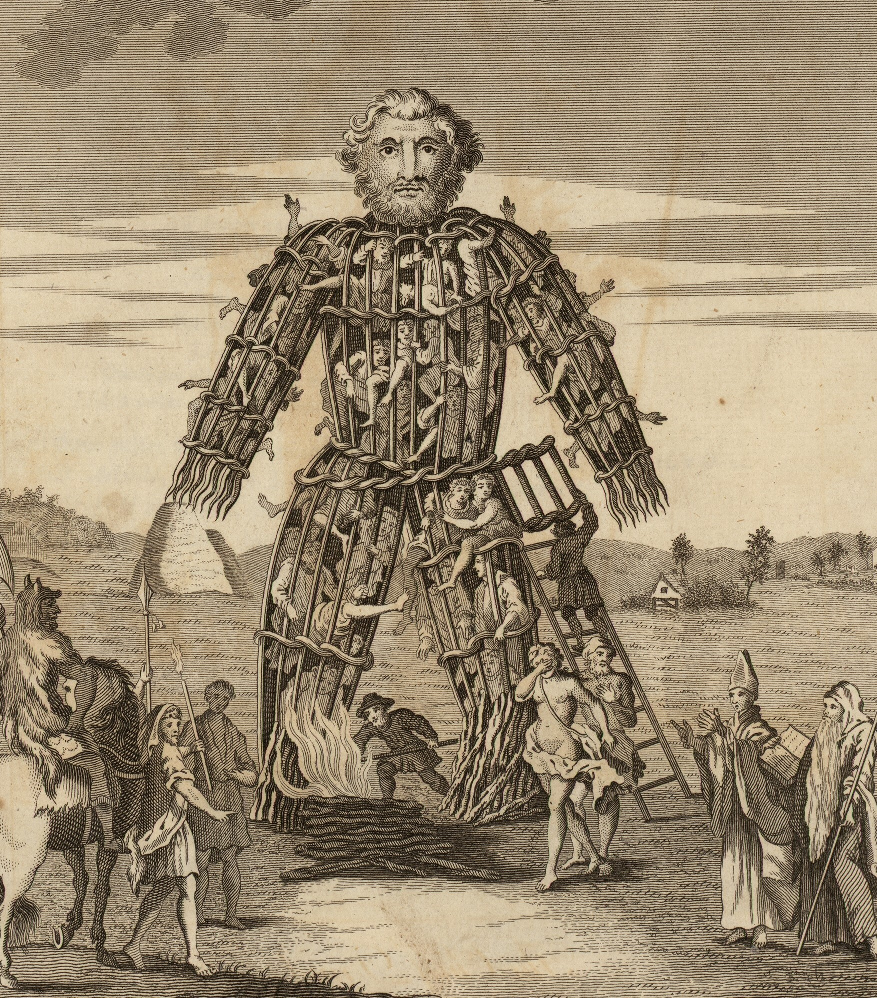
\includegraphics[width=0.3\textwidth]{graphics/ch2Figs/t_pennant.pdf}
  \end{center}
    \caption{An engraving depicting acolytes of the tidyverse burning live sacrifices, captive within a large wicker effigy, to appease their deities \parencite{Pennant1784}.}
    \label{fig:ch2_wicker}
\end{wrapfigure}

Then came the tidyverse. A revelation. A collection of mystical and cohesive R packages, summoned into the light by Hadley Wickham and his coven of arcane programmers \parencite{Wickham2019}. Their sorcery brought order to the chaos, shaping the wild, unruly cosmos of R into something usable—something powerful.

The tidyverse became a gateway for common folk, allowing them to twist, shape, and visualize data with an ease once reserved for only the most privileged elite. Though once viewed as complex and heretical \parencite{Muenchen}, the tidyverse has become an essential craft, passed from hand to hand, spreading like whispers in the dark. The art of tidy data flourished, growing stronger through collaboration, trial, and sacrifice.

Make no mistake: sacrifice is inevitable (see Figure \ref{fig:ch2_wicker}). There will be frustration, moments of despair, and the occasional bout of madness. Yet the tidyverse offers an unparalleled path to power, a means to harness the dark beauty of data in ways that defy the purposeless void.

And so, we begin our journey here—with the basics of data plotting. Like any great practitioner of forbidden arts, you must first master the grimoires and sigils of power. The tidyverse is no mere toolset; it is a pact, a ritual binding you to its magic. To wield such dark sorcery without understanding is to invite chaos—but with mastery, you will bend the data to your will, carving order from the void itself.

\normalfont

\section{Worshiping at the alter of the tidyverse}
\label{sec:tidyverse}

As described by its website (\url{https://www.tidyverse.org/}), the \gls{tidyverse} is an opinionated collection of R packages that share an underlying design philosophy. Each package can be installed individually, though most find it easiest to install every package within the scope of the tidyverse all at once.


\begin{inR}
install.packages("tidyverse")
library(tidyverse)
\end{inR}

% \begin{outR}
% -- Attaching core tidyverse packages -- tidyverse 2.0.0 --
%  dplyr     1.1.4      readr     2.1.5
%  forcats   1.0.0      stringr   1.5.1
%  ggplot2   3.5.1      tibble    3.2.1
%  lubridate 1.9.3      tidyr     1.3.1
%  purrr     1.0.2     
% -- Conflicts -------------------- tidyverse_conflicts() --
%  dplyr::filter() masks stats::filter()
%  dplyr::lag()    masks stats::lag()
%  Use the conflicted package to force all conflicts to
%  become errors
% \end{outR}

\begin{outR}
── Attaching core tidyverse packages ──────────────────────────────── tidyverse 2.0.0 ──
dplyr     1.1.4     readr     2.1.5
forcats   1.0.0     stringr   1.5.1
ggplot2   3.5.1     tibble    3.2.1
lubridate 1.9.3     tidyr     1.3.1
purrr     1.0.2     
── Conflicts ────────────────────────────────────────────────── tidyverse_conflicts() ──
dplyr::filter() masks stats::filter()
dplyr::lag()    masks stats::lag()
Use the conflicted package to force all conflicts to become errors
\end{outR}

While the above code installs all the packages, running \R{library(tidyverse)} only loads the the nine ``core'' packages:  \textit{ggplot2}, \textit{dplyr}, \textit{tidyr}, \textit{readr}, \textit{purr}, \textit{tibble}, \textit{stringr}, \textit{forcats}. Other tidyverse packages, such as \textit{readxl}, will need to be loaded separately using the \R{library()} function.

Speaking for the beginner, it will be noticed that when the tidyverse is loaded, not only is there a confirmation of what packages (and their versions) have been loaded, but there is also a list of ``conflicts'' displayed in the output.\footnote{Most packages will not display this information for you quite so nicely as the tidyverse does, so pay attention to any messages you receive using the \R{library()} function.} For instance, two functions from the \textit{dplyr} package, \R{filter()} and \R{lag()}, have the same name as pre-existing functions within R and, when you load a package with a conflict like this, precedence is always given to the most recently loaded package. This means, when you use the \R{filter()} function for example, R is going to use the version belonging to \textit{dplyr}, not the original version that was a part of base R's \textit{stats} package (which is pre-loaded each time you use R). Though you can still use that original version in the following manner: \R{package\_name::function\_name()}.  For example, \R{stats::filter()}. 

As a whole, the tidyverse will not solve all your problems, but it will come damn close. Admittedly, and this is particularly true for beginners, much of what the tidyverse offers will not be needed in your daily programming rituals, but will come in handy when least expected.

\section{Plotting with R}

A core component of any GOOD DATA ANALYSIS obviously involves visualizing your data. As you progress through the various topics in this book, specific types of plots and their uses will be discussed in detail; however, for the time being, it will be helpful to get an intuitive sense of how plotting works with R generally. Thus, what follows in this section is intended to help you understand the logic of plotting with R. The goal at this point is not to make you an expert; rather, it is to provide beginners with a base level of knowledge.

By itself, base R comes with a stock set of functions for plotting data. To illustrate we can run the following code to produce a nice looking histogram ...

\begin{inR}
x <- rnorm(10000)
hist(x)
\end{inR}
\vspace{1em}

\noindent
In the case of the above code, the function \R{rnorm()} is just generating 10,000 random values.\footnote{The random values are technically coming from a ``standard normal'' distribution (hence the ``norm'' in \R{rnorm}), but don't worry about that for now.} The function \R{hist(x)}, is simply plotting those values as a histogram.  Running the code should generate an output similar to what you see below.

\begin{figure}[H]
\centering
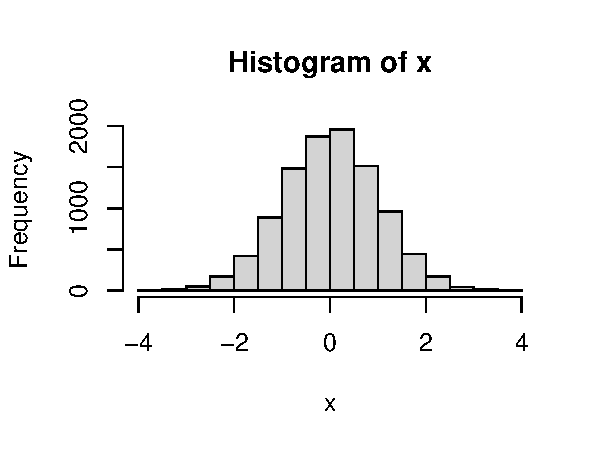
\includegraphics[scale = 0.75, trim={0 5mm 0 0},clip]{graphics/ch2Figs/base_hist.pdf}
\caption{An example of base R's plotting functions.}
\label{fig:base_hist}
\end{figure}

R's base plotting functions offer a convenient means of producing simple quality plots and can be very efficient when working with \gls{univariate data} or \gls{bivariate data}. This is data which consists of only one (uni) or two (bi) variables, respectively. However, a lot of research is concerned with analysing \gls{multivariate data}. This is data consisting of two or more \glspl{response variable} alongside other explanatory variables. Each additional variable adds ever increasing amounts of complexity and nuance to your data and, by extension, the plots you use to visualizing those data.  The stock set of plotting functions R offers can accommodate these more complex scenarios; however, that level of accommodation is heavily dependent on the users proficiency with R.  For this reason, this book will adopt the practice of ignoring R's base plotting functions, and instead rely on well-known R package called \textit{ggplot2} which is among the most venerated portions of the tidyverse.   

The \textit{``gg''} in \textit{ggplot2} stands for ``grammar of graphics'' and provides users with a logical framework for the construction of plots within R.  The term ``grammar'' here is likely to conjure up long forgotten traumas of boring English and Language Arts lessons, but do not fear, the use of the term grammar is really just to emphasize that \textit{ggplot2} is constructed in a way that allows users to build plots of various kinds in a consistent and efficient manner that is easily tailored to their specific needs.  This is in contrast to how plotting in software works generally, where you are frequently stuck trying to fit a square peg (your data) into a circular hole (the software's narrow conception of how data should be presented).

\clearpage
The easiest way to understand how \textit{ggplot2} works is to simply dive in and use it. Along the way, we will also learn a little bit more about R and data manipulation. However, a disclaimer is perhaps useful here:

\begin{displayquote}
\centering
\headingfont
   This chapter contains a large variety of functions and strategies for plotting data with \textit{ggplot2}. The reader would do well to head the advice provided on page 1.
\end{displayquote}

The first thing to do will be to ensure that \textit{ggplot2} has been installed into our computer's library of packages and loaded so we can access its functions. As mentioned in section \ref{sec:tidyverse}, if you have installed and loaded the tidyverse, this is already done, but if you chose not to do that,\footnote{Shame on you.} \textit{ggplot2} can be installed and loaded as a standalone package as well.

\begin{inR}
install.packages("ggplot2")
library(ggplot2)
\end{inR}

\subsection{An example data set: msleep}

Before we can plot anything, we need something to plot.  In addition to its large set of plotting functions, the \textit{ggplot2} package also provides a few illustrative data sets.\footnote{Base R comes with a nice collection of data sets as well. To obtain a list you need only run the function \R{data()}.  To obtain the list of data sets for \R{ggplot2} you need only include the package name as an argument in this function: \R{data(package = "ggplot2")}} We will work with the \R{msleep} data set, which provides a variety of measurements relevant to the sleep behaviour of a wide range of mammals. To access the data you need only run the code \R{msleep}, which will output a $83 \times 11$ data frame.\footnote{Technically we are looking at a ``tibble'', which is the ``tidyverse's'' own take on a data frame. For our present purposes though, this is a distinction without a difference.} Given the limited space available in the console window, the data frame is going to be truncated substantially. Thus, if you would like to view the entire data set, you can utilize R's \R{View()} function, which will display the data in a separate spreadsheet style window.

\begin{inR}
msleep # print data to console
View(msleep) # view the data in a spreadsheet-style window
\end{inR}

\vspace{2em}

\begin{table}[!h]
\centering
\resizebox{\textwidth}{!}{%
\begin{tabular}{lllllrrrrrr}
\toprule
name & genus & vore & order & conservation & sleep\_total & sleep\_rem & sleep\_cycle & awake & brainwt & bodywt\\
\midrule
\cellcolor{gray!10}{Cheetah} & \cellcolor{gray!10}{Acinonyx} & \cellcolor{gray!10}{carni} & \cellcolor{gray!10}{Carnivora} & \cellcolor{gray!10}{lc} & \cellcolor{gray!10}{12.1} & \cellcolor{gray!10}{NA} & \cellcolor{gray!10}{NA} & \cellcolor{gray!10}{11.9} & \cellcolor{gray!10}{NA} & \cellcolor{gray!10}{50.000}\\
Owl monkey & Aotus & omni & Primates & NA & 17.0 & 1.8 & NA & 7.0 & 0.016 & 0.480\\
\cellcolor{gray!10}{Mountain beaver} & \cellcolor{gray!10}{Aplodontia} & \cellcolor{gray!10}{herbi} & \cellcolor{gray!10}{Rodentia} & \cellcolor{gray!10}{nt} & \cellcolor{gray!10}{14.4} & \cellcolor{gray!10}{2.4} & \cellcolor{gray!10}{NA} & \cellcolor{gray!10}{9.6} & \cellcolor{gray!10}{NA} & \cellcolor{gray!10}{1.350}\\
Greater short-tailed shrew & Blarina & omni & Soricomorpha & lc & 14.9 & 2.3 & 0.133 & 9.1 & 0.000 & 0.019\\
\cellcolor{gray!10}{Cow} & \cellcolor{gray!10}{Bos} & \cellcolor{gray!10}{herbi} & \cellcolor{gray!10}{Artiodactyla} & \cellcolor{gray!10}{domesticated} & \cellcolor{gray!10}{4.0} & \cellcolor{gray!10}{0.7} & \cellcolor{gray!10}{0.667} & \cellcolor{gray!10}{20.0} & \cellcolor{gray!10}{0.423} & \cellcolor{gray!10}{600.000}\\
Three-toed sloth & Bradypus & herbi & Pilosa & NA & 14.4 & 2.2 & 0.767 & 9.6 & NA & 3.850\\
\cellcolor{gray!10}{Northern fur seal} & \cellcolor{gray!10}{Callorhinus} & \cellcolor{gray!10}{carni} & \cellcolor{gray!10}{Carnivora} & \cellcolor{gray!10}{vu} & \cellcolor{gray!10}{8.7} & \cellcolor{gray!10}{1.4} & \cellcolor{gray!10}{0.383} & \cellcolor{gray!10}{15.3} & \cellcolor{gray!10}{NA} & \cellcolor{gray!10}{20.490}\\
Vesper mouse & Calomys & NA & Rodentia & NA & 7.0 & NA & NA & 17.0 & NA & 0.045\\
\cellcolor{gray!10}{Dog} & \cellcolor{gray!10}{Canis} & \cellcolor{gray!10}{carni} & \cellcolor{gray!10}{Carnivora} & \cellcolor{gray!10}{domesticated} & \cellcolor{gray!10}{10.1} & \cellcolor{gray!10}{2.9} & \cellcolor{gray!10}{0.333} & \cellcolor{gray!10}{13.9} & \cellcolor{gray!10}{0.070} & \cellcolor{gray!10}{14.000}\\
Roe deer & Capreolus & herbi & Artiodactyla & lc & 3.0 & NA & NA & 21.0 & 0.098 & 14.800\\
\bottomrule
\end{tabular}}
\caption{First 10 rows of the \R{msleep} data}
\label{tab:msleep}
\end{table}






















\noindent
Table \ref{tab:msleep} shows the first 10 rows and 6 columns of \R{msleep} data.  Looking more closely at the data, we can see a variety of variables (the column names) that are, for the most part, self explanatory.
In this case, the column names represent distinct variables that have been measured and, particularly with larger data frames that cannot be adequately printed to the console, it is often useful to have R list out the name of each column. We can do this quite easily using the \R{names()} function.

\begin{inR}
names(msleep)
\end{inR}
\begin{outR}
 [1] "name"         "genus"        "vore"        
 [4] "order"        "conservation" "sleep_total" 
 [7] "sleep_rem"    "sleep_cycle"  "awake"       
[10] "brainwt"      "bodywt"   
\end{outR}

Now, while the names of each column are self-explanatory, the elements of each column are perhaps less so.  For instance, in the \R{\$sleep\_total} column, are we looking at values in minutes, hours, or days? In the \R{\$conservation} column we can see a number of abbreviations such as \R{lc}, \R{nt}, \R{vu}, and so on. What do we make of those? A good starting point for answering these questions is to check the documentation associated with the data set, which all CRAN packages are required to include. This can be accessed in the usual way with a \R{?}

\begin{inR}
?msleep
\end{inR}
\vspace{1em}

\noindent
Inspecting the documentation, we can see that \R{\$sleep\_total} is given in hours and that the column \R{\$conservation} indicates ``the conservation status of the animal.''  Admittedly, concerning this latter column, that does not tell us too much, but it does at least give us a starting point for understanding what those values might represent.  In all likelihood, we are seeing abbreviations for the IUCN's (International Union for Conservation of Nature) species ranking. 

\begin{itemize}
\setlength\itemsep{-1em}
    \item \R{lc} = Least Concern
    \item \R{nt} = Near Threatened
    \item \R{vu} = Vulnerable
    \item \R{en} = Endangered
    \item \R{cd} = Conservation Dependent
\end{itemize}

Using a \gls{scatter plot} as a basic starting point, we will graph the relationship between the variables body weight (kg) and sleep total (hours).  These are represented by the columns \R{\$bodywt} and \R{\$sleep\_total} respectively. 

\section{Adding layers}

\textit{ggplot2} constructs plots by adding visual layers on top of one another. The first layer is the grid upon which our scatter plot's points will appear.  To generate this first layer we can simply type ...

\begin{inR}
ggplot(data = msleep, aes(x = bodywt, y = sleep_total))
\end{inR}

\vspace{2em}

\begin{figure}[H]
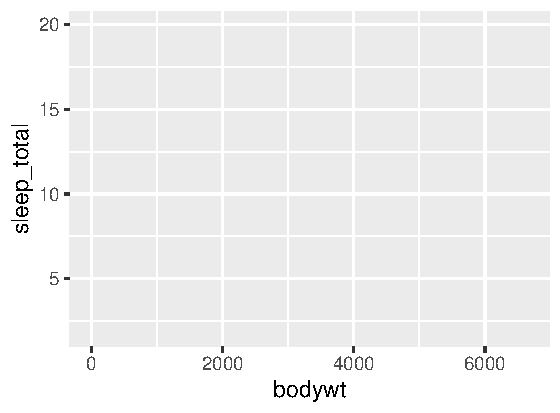
\includegraphics[scale = 0.75]{graphics/ch2Figs/ggEx_1.pdf}
\label{fig:ggEx_1.pdf}
\end{figure}

\noindent
Looking at the \R{ggplot()} function we typed, we can see that the argument \R{data} tells \textit{ggplot2} where the data is coming from - in this case it is coming from the \R{msleep} data frame.  The \R{x} and \R{y} arguments are telling \textit{ggplot2} what variables/columns should be mapped to the x and y axis respectively.  Notice that, not only has \textit{ggplot2} labelled the axis accordingly, but it has also given them scales that correspond to size of the values found in both columns.

\clearpage
Next we will, quite literally, add (\R{+}) a layer of points on top of this by typing \R{+ geom\_point()}. The term ``geom'' here is just an abbreviation for ``geometric object'', and points are one of many different types of geometric object \textit{ggplot2} recognizes.

\begin{inR}
ggplot(data = msleep, aes(x = bodywt, y = sleep_total)) +
  geom_point()
\end{inR}

\vspace{2em}

\begin{figure}[H]
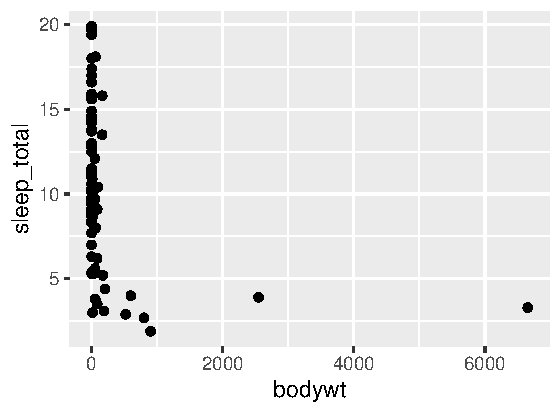
\includegraphics[scale = 0.75]{graphics/ch2Figs/ggEx_2.pdf}
\label{fig:ggEx_2.pdf}
\end{figure}

\noindent
At this juncture, it is worth taking a moment to talk about how this code we have written has been organized. Here we placed \R{geom\_point()} on a new line and indented it.  This was not something we strictly had to do.  We could have put everything on a single line like so ...

\begin{inR}
ggplot(data = msleep, aes(x = bodywt, y = sleep_total)) + geom_point()
\end{inR}

\vspace{1em}

\noindent
But, particularly as we add more customization to the plot, this style of writing becomes hard to read. The (tidyverse's) \href{https://style.tidyverse.org/syntax.html#long-lines}{R style guide} recommends that no line of code exceed 80 characters, which is the advice most of the R community adheres to. In fact, Rstudio can be configured to display a margin representing the 80 character limit: (\textit{Tools $\rightarrow$ Global Options $\rightarrow$ Code $\rightarrow$ Display}). To ensure that you do not exceed limit with larger blocks of code, it is worth remembering that you can always move portions of code to a new line after a comma, operator, or unclosed parentheses. The indentation we used is purely to guide the eye in recognizing that \R{geom\_point()} belongs to a larger block of code.\footnote{While the R programming language allows users to indent code with reckless abandon, some programming languages, such as \textit{Python}, require it to be used in very specific ways.}

\subsection{Inspecting potential outliers}

At present, the plot does not look like much.  There are numerous points scattered between 0 and 1000, and a couple of very extreme points beyond which are skewing the x-axis scale and making the majority of the data difficult to visualize. Given how rare and extreme these two values appear, we should inspect them to ensure that they are not errors within the data set (i.e., ensure that there is not a 2500 kg mouse, bird, or other such abomination in our data set). To accomplish this, most people will instinctively try to scan the data frame's 83 rows one by one with their eyes. Obviously, that strategy will be slow, inefficient, and highly prone to error.  A better strategy is to have R isolate these values using the \R{filter()} function which is part of the tidyverse's \textit{dplyr} package.\footnote{Base R has a (more or less) equivalent function \R{subset()} that we could use as well. There are reasons for preferring \R{filter()}, but in this context there is no advantage to using either.}  We simply give the function our data frame, and then specify a logical rule to subset by. In this case we will tell the function to show us all the rows that have a body weight greater than 2000.

\begin{inR}
filter(msleep, bodywt > 2000)
\end{inR}

\begin{outR}
# A tibble: 2 × 11
  name             genus     vore  order       conservation sleep_total
  <chr>            <chr>     <chr> <chr>       <chr>              <dbl>
1 Asian elephant   Elephas   herbi Proboscidea en                   3.9
2 African elephant Loxodonta herbi Proboscidea vu                   3.3
# 5 more variables: sleep_rem <dbl>, sleep_cycle <dbl>, awake <dbl>, 
# brainwt <dbl>, bodywt <dbl>
\end{outR}

\vspace{1em}

A quick glance at the output reveals that these two points represent the Asian and African elephant respectively.  Thus, while these values are quite extreme and do not seem to be terribly representative of the data as a whole, they are not mistakes and therefore should remain in the data set.  However, this begs the question, how do we visualize this data adequately with such odd scaling?

\clearpage
\subsection{Logarithms}

A common strategy in cases like this where larger values tend to become more and more extreme (i.e., exhibit some kind of exponential growth) is to plot the logarithm of the values. As a refresher of high school mathematics, logarithms are essentially exponents in reverse. For example:

\vspace{-2em}

$$10^3 = 10 \times 10 \times 10 = 1000$$

\vspace{-1em}

\noindent
A \textit{base-10} logarithm simply undoes this process by stating how many 10s it takes to create 1000.

\vspace{-2em}

$$\log_{10}(1000) = 3$$

\vspace{-1em}

\noindent
A \textit{base-2} logarithm asks: how many 2s are required to create 1000?

\vspace{-2em}

$$\log_{2}(1000) \approx 9.966$$

\vspace{-1em}

\noindent
Thus, $2^{9.966} \approx 1000$.  

%\vspace{-1em}

\noindent
A \textit{natural} logarithm uses a base denoted as $e$ (Euler's Number), which is approximately 2.71828.

\vspace{-2em}

$$\log_e(1000) \approx 6.908$$

\vspace{-1em}

\noindent
Base-10, base-2, and natural logarithms represent the most widely used types of logarithms,\footnote{For clarity and consistency the natural logarithm of 1000 has been written $\log_e(1000)$, but it is common practice to identify natural logarithms using ``$\ln$''. E.g., $\ln{(1000) \approx 6.908}$.} but you can technically use any base you desire.  As seen below, the use of logarithms in R is very straightforward.

\begin{inR}
log10(1000) # Base-10 function
log2(1000) # Base-2 function
log(1000) # Natural log
log(1000, base = 666) # Pick your own base
\end{inR}
\begin{outR}
[1] 3
[1] 9.965784
[1] 6.907755
[1] 1.062521
\end{outR}

A base-10 logarithm is generally considered the most intuitive so we will use that. There are various ways to incorporate a logarithmic scale on our plot's axis, but perhaps the safest way is to simply add a new column of $\log_{10}$ values to our dataframe and plot that instead of the standard \R{\$bodywt} column.

\begin{inR}
# Add new column of log bodywt values.
msleep$bodywt_log10 <- log10(msleep$bodywt)

# Re-plot the data
ggplot(msleep, aes(x = bodywt_log10, y = sleep_total)) +
  geom_point()
\end{inR}

\vspace{2em}

\begin{figure}[H]
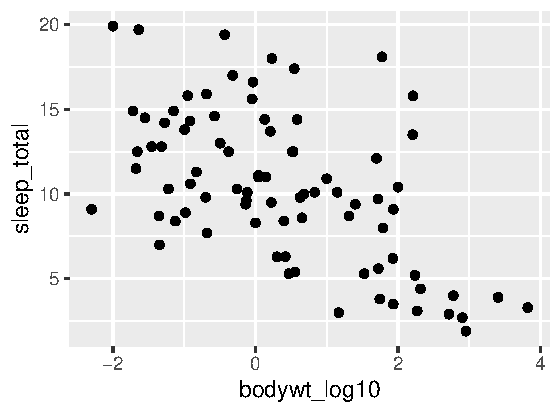
\includegraphics[scale = 0.75]{graphics/ch2Figs/ggEx_3.pdf}
\label{fig:ggEx_3.pdf}
\end{figure}

\section{Aesthetics}

Geometric objects in \textit{ggplot2}, like the point geom, all have various traits, like their size, shape, and colour that can be customized.  In the language of \textit{ggplot2}, these are referred to as \gls{aesthetics}.  For example, we can customize the points in the following way ...

\begin{inR}
ggplot(msleep, aes(x = bodywt_log10, y = sleep_total)) +
  geom_point(size = 3, 
             shape = 4, 
             colour = "blue", 
             stroke = 1.5)
\end{inR}

\begin{figure}[!h]
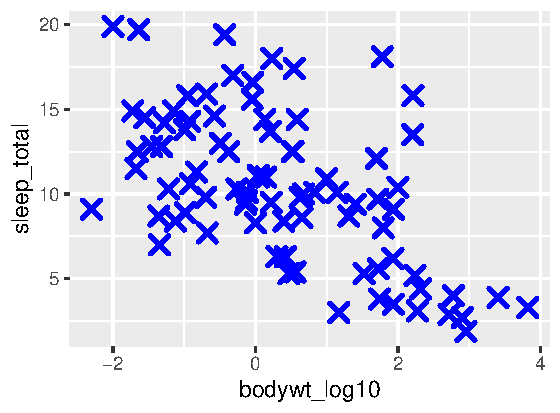
\includegraphics[scale = 0.75]{graphics/ch2Figs/ggEx_5.pdf}
\end{figure}

\begin{mdframed}[nobreak=true, style = miscFrame, frametitle = \Large\IMFellEnglish Box 2.1: An alternative way to scale]
\IMFellEnglish

In the previous example, the logarithm was applied by creating a new column of x-axis values and plotting that. However, this means that, if you want to interpret the numbers in their original units, you need to calculate 10\textsuperscript{\textit{x}}, which can be annoying.  

\noindent An alternative strategy would be to keep the \R{\$bodywt} column as is and just scale the plot's axis itself to increment logarithmically, which \textit{ggplot2} will do straightforwardly.

\begin{inR}
ggplot(msleep, aes(x = bodywt, y = sleep_total)) +
  geom_point() +
  scale_x_continuous(trans = "log10")
\end{inR}

\vspace{1em}

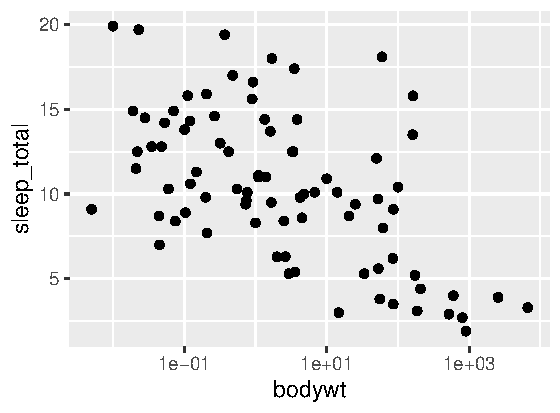
\includegraphics[scale = 0.7]{graphics/ch2Figs/ggEx_4.pdf}

\noindent The advantage of this method is you can look at a point's value on the x-axis and know immediately that it corresponds to a weight of \textit{x} kg. The drawback is you may end up with excessively small or large values on the axis, hence the \href{https://www.mathsisfun.com/numbers/scientific-notation.html}{\textit{scientific notation}} you see in the plot.

\end{mdframed}

\clearpage

With a bit of experimentation, it should be apparent how the arguments \R{size} and \R{stroke} work in the above example; however, the \R{shape} and \R{colour} arguments are slightly less intuitive.\footnote{If you accidentally omit the ``u'' when typing ``colour,'' \textit{ggplot2} will still understand what you mean, even though it isn't correct English.} R comes with a variety of point shapes (technically called ``plotting characters'' or ``\gls{pch}'' symbols for short) that are denoted by numbers. The various possibilities are depicted in Figure \ref{fig:points.pdf}.  In this case, number 4 is an $\times$.  Notably, the last five plotting characters (21 through 25) incorporate both a \R{colour} aesthetic for their edges and a \R{fill} aesthetic. All the other symbols only require a \R{colour} aesthetic to be specified.

\begin{inR}
ggplot(msleep, aes(x = bodywt_log10, y = sleep_total)) +
  geom_point(
    size = 3,
    shape = 25,
    colour = "black",
    stroke = 1.5,
    fill = "red"
  )
\end{inR}

\vspace{2em}

\begin{figure}[H]
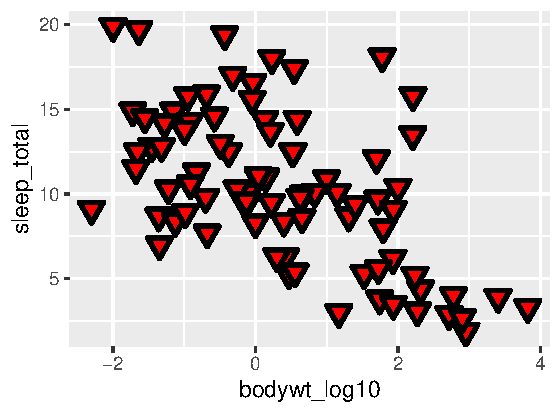
\includegraphics[scale = 0.75]{graphics/ch2Figs/ggEx_6.pdf}
\end{figure}

\noindent
The plotting characters shown in Figure \ref{fig:points.pdf} are just a few of the options available. For instance, by using values ranging between 32 and 127, you can display a variety of ASCII characters. Additionally, you can specify a particular character instead of providing a numeric value, e.g., \R{shape = "\&"}.

\bigskip

\begin{figure}[htbp]
\centering
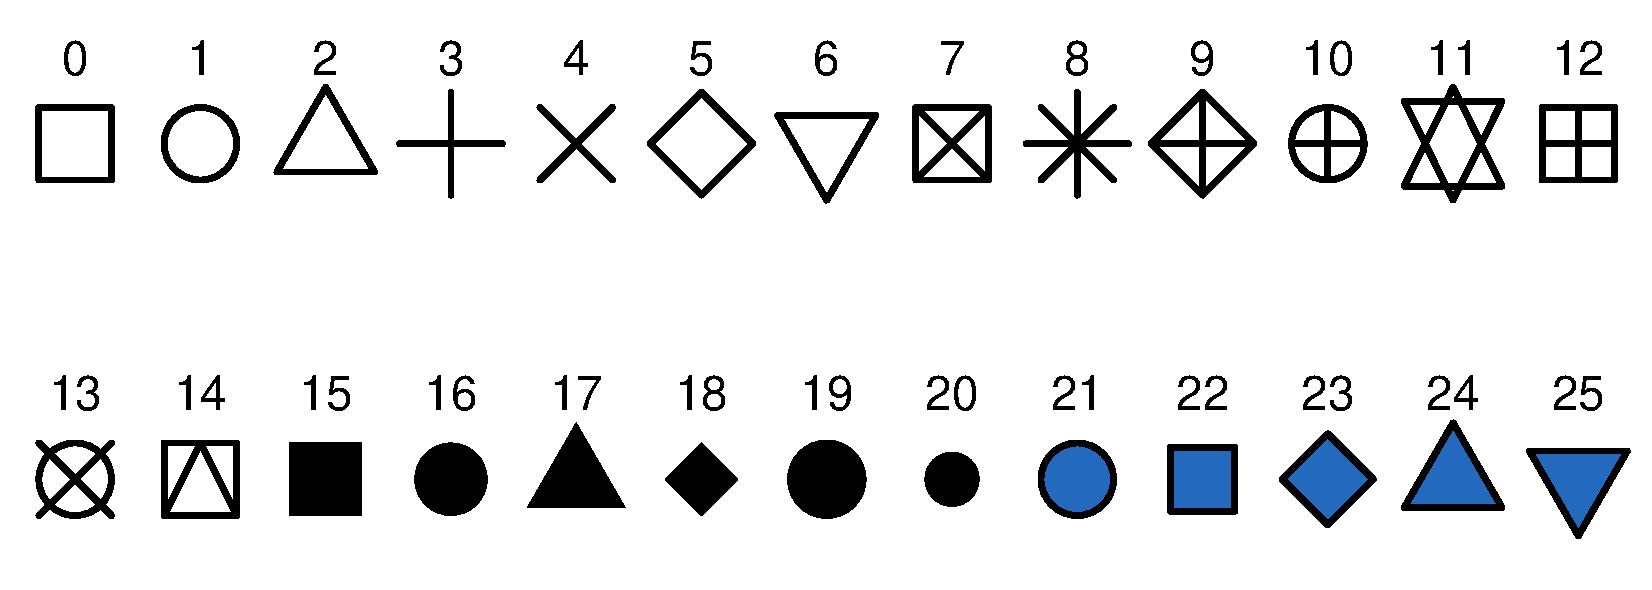
\includegraphics[scale = 0.5]{graphics/ch2Figs/pch.pdf}
\caption{R Plotting Characters}
\label{fig:points.pdf}
\end{figure}

\bigskip

\noindent
In the above examples we specified a desired colour by typing the name of a primary colour, but we are not limited to just using primary colours. R comes with a built in set of 657 differently named colours.  You can obtain the full list of colour names by running \R{colors()}.  R also has a built-in demo of these colours you can run to get a visual representation of each.  Simply run the command \R{demo("colors")}. 

Alternatively, instead of typing a colour name, you can use a hexadecimal value (also referred to as a ``hex code'' or ``hex value'') that represents a specific colour. For example, the hex value \R{"\#FFC0CB"} represents the colour pink. Hexadecimal values offer the user a lot of nuance when it comes to colour selection and, in most cases, the simplest way of finding an appropriate hex value is to consult one of the many websites devoted to colour codes and colour theory (i.e., do an internet search). However, if you would like to understand the theory behind hex codes and why they are used, see Box 2.2.

\begin{mdframed}[nobreak = true, style = miscFrame, frametitle = \Large\IMFellEnglish Box 2.2: Hexadecimal Notation for Colours]
\IMFellEnglish

Hexadecimal values are simply numbers that use a base-16 counting method. In other words, in the world of hexadecimals, there are 16 different numbers that are used to count with, instead of the typical 10 numbers (0:9), you were probably raised to use. These are 

\vspace{1em}

\begin{table}[H]
\centering
\IMFellEnglish
\begin{tabular}{|l|l|l|l|l|l|l|l|l|l|l|l|l|l|l|l|l|}
\hline
\textbf{Decimal}     & 0 & 1 & 2 & 3 & 4 & 5 & 6 & 7 & 8 & 9 & 10 & 11 & 12 & 13 & 14 & 15 \\ \hline
\textbf{Hexadecimal} & 0 & 1 & 2 & 3 & 4 & 5 & 6 & 7 & 8 & 9 & A  & B  & C  & D  & E  & F  \\ \hline
\end{tabular}
\end{table}

\noindent
Because of their larger base, a single hexadecimal digit can store more information than a conventional base-10 digit can.  For instance, if a computer stores various gradations of the colour red using just two digits, that only allows for 100 (10 x 10) different reds. Using hexadecimals you can have 256 (16 x 16) reds, with just two digits.  Thus, if a colour is some combination of red, green, and blue, and each is stored using two hexadecimal digits that gives you 256\textsuperscript{3} = 16,777,216 colours as opposed to the meagre 100\textsuperscript{3} = 1,000,000 you would have using the inferior base-10 counting method.

\noindent To use hexadecimals to represent colour, two digits are assigned to red (RR), green (GG) and blue (BB), in that order like so \R{"\#RRGGBB"}.  Smaller values are darker, and larger values are brighter.  Consequently, black is represented as \R{"\#000000"} and white is represented as \R{"\#FFFFFF"}. Thus, if you want the \enquote{purest} red, you would input \R{"\#FF0000"}, the purest green would be \R{"\#00FF00"}, and the purest blue would be \R{"\#0000FF"}.
\end{mdframed}

\subsection{Aesthetics by variable}

In the above examples, the aesthetic changes we made to the plots affected all of the points. In the language of \textit{ggplot2}, we would say that the aesthetics were mapped to all the points. However, it is often necessary to visually break up the points according to one of the other variables in your data.  For instance, we could colour the points in our plot according to the categories in the data's \R{\$vore} column.

\begin{inR}
ggplot(msleep, aes(x = bodywt_log10, y = sleep_total)) +
    geom_point(size = 3, aes(colour = vore))
\end{inR}

\vspace{2em}

\begin{figure}[H]
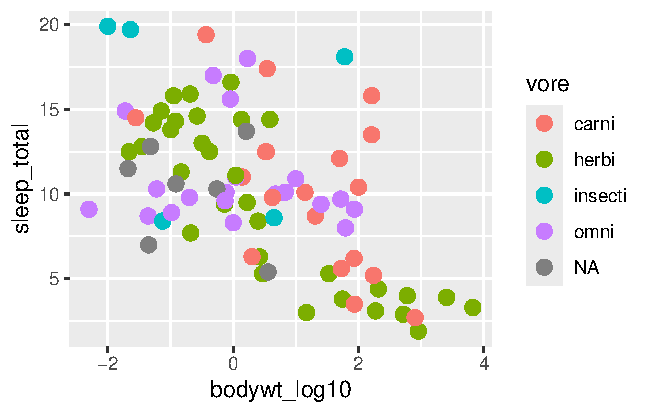
\includegraphics[scale = 0.75]{graphics/ch2Figs/ggEx_7.pdf}
\end{figure}

\noindent
Notice that the plot's legend shows an ``NA'' category. This is because there are \R{NA} values found within the \R{\$vore} column (run \R{msleep\$vore} to see them). Thus, the legend's ``NA'' category represents values that we have body weight and sleep total information for, but we do not know what those animals diet consists of and therefore cannot categorize them properly.\footnote{To see the full list of animals who have a missing \R{\$vore} value, you can run \R{filter(msleep, is.na(vore))}. This will show all the rows for which \R{is.na(vore)} evaluates to \R{TRUE}.} So instead of referring to this category as ``NA'', we could refer to these as ``unknown.'' All we need to do is change the \R{NA} values in the data frame's \R{\$vore} column to character values that read \R{"unknown"}. This can be done simply by using the \R{ifelse()} function, which tests a statement you write. If that statement is true, it produces a value you have specified, if it false, then it produces an alternative value you have specified.  In other words, it works like this: 

\noindent
\R{ifelse(test, \textit{true result}, \textit{false result})}.

\noindent
In this case, we want to test \textit{if} the value in each row \textit{is} an \R{NA} value or not. Recall that the function \R{is.na()} tells us whether the value of a vector is an \R{NA} value or not.

\begin{inR}
is.na(msleep$vore)
\end{inR}
\begin{outR}
 [1] FALSE FALSE FALSE FALSE FALSE FALSE FALSE
 [8]  TRUE FALSE FALSE FALSE FALSE FALSE FALSE
 [15] ...
\end{outR}

\clearpage
\noindent
Thus, we can use that as the ``test'' in the \R{ifelse()} function.

\begin{inR}
ifelse(is.na(msleep$vore), "unknown", msleep$vore)
\end{inR}

\begin{outR}
 [1] "carni"   "omni"    "herbi"   "omni"    "herbi"   "herbi"   "carni"  
 [8] "unknown" "carni"   "herbi"   "herbi"   "herbi"   "omni"    "herbi"  
[15] "omni"    "omni"    "omni"    "carni"   "herbi"   "omni"    "herbi"  
[22] "insecti" "herbi"   "herbi"   "omni"    "omni"    "herbi"   "carni"  
[29] "omni"    "herbi"   "carni"   "carni"   "herbi"   "omni"    "herbi"  
[36] "herbi"   "carni"   "omni"    "herbi"   "herbi"   "herbi"   "herbi"  
[43] "insecti" "herbi"   "carni"   "herbi"   "carni"   "herbi"   "herbi"  
[50] "omni"    "carni"   "carni"   "carni"   "omni"    "unknown" "omni"   
[57] "unknown" "unknown" "carni"   "carni"   "herbi"   "insecti" "unknown"
[64] "herbi"   "omni"    "omni"    "insecti" "herbi"   "unknown" "herbi"  
[71] "herbi"   "herbi"   "unknown" "omni"    "insecti" "herbi"   "herbi"  
[78] "omni"    "omni"    "carni"   "carni"   "carni"   "carni"  
\end{outR}

When you run the above code, the \R{ifelse()} function scans each row of the \R{\$vore} column and evaluates whether \R{is.na(msleep\$vore)} is \R{TRUE}. If it is true, it replaces the existing \R{NA} value with \R{"unknown"}. However, if it \R{FALSE}, it leaves it as the original value (this is why we wrote \R{msleep\$vore} after the second comma). The end result is a vector of values that we can use to replace the existing \R{\$vore} column with.

\begin{inR}
msleep$vore <- ifelse(is.na(msleep$vore), "unknown", msleep$vore)
\end{inR}

\vspace{1em}

\noindent
Now, when we re-plot the graph, we get something much more sensible ....

\begin{inR}
ggplot(msleep, aes(x = bodywt_log10, y = sleep_total)) +
    geom_point(size = 3, aes(colour = vore))
\end{inR}
\vspace{2em}
\begin{figure}[H]
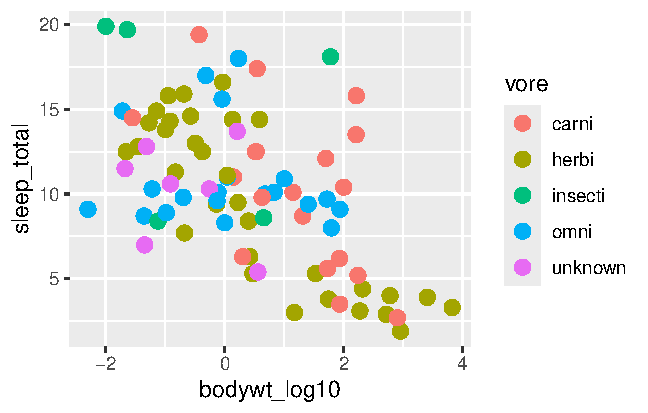
\includegraphics[scale = 0.75]{graphics/ch2Figs/ggEx_8.pdf}
\end{figure}

When plotting, it is usually inadvisable to \textit{only} adjust the colour of your points because a sizeable portion of the population has some form of colour vision deficiency (a.k.a., colour blindness). And while there are ``colourblind friendly'' palettes we can use, there is no universal palette that works optimally for all cases of colour deficiency. Consequently, the best practice is to have each category be represented by a distinct shape. 

\begin{inR}
ggplot(msleep, aes(x = bodywt_log10, y = sleep_total)) +
    geom_point(size = 3, aes(colour = vore, shape = vore))
\end{inR}

\vspace{2em}

\begin{figure}[H]
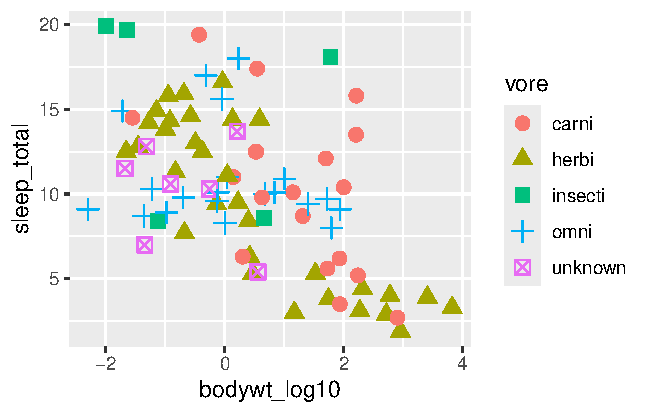
\includegraphics[scale = 0.75]{graphics/ch2Figs/ggEx_9.pdf}
\end{figure}

\section{Displaying trends}

Notice that the data points appear to trend downward as you move from left to right on the x-axis. In other words, as body weight increases, you tend to see decreases in sleep total. By simply adding a second geom, called \R{geom\_smooth()}, we can use a line of best fit to represent (i.e., model) this trend.

\begin{inR}
ggplot(msleep, aes(x = bodywt_log10, y = sleep_total)) +
    geom_point(size = 3, aes(colour = vore, shape = vore)) +
    geom_smooth()
\end{inR}
\vspace{2em}
\begin{figure}[H]
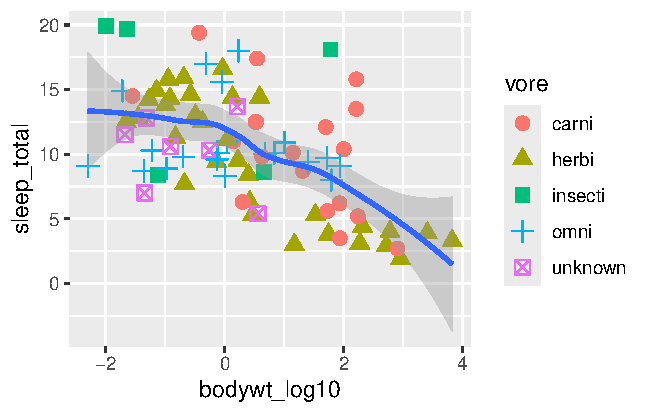
\includegraphics[scale = 0.75]{graphics/ch2Figs/ggEx_10.pdf}
\end{figure}

The shaded grey area represents a statistic called the \textit{standard error} and the line was drawn using a fancy smoothing method called \textit{local polynomial regression fitting}, but we can use a more common regression line as well and modify various aspects of it just like we had done earlier using \R{geom\_point()}.

\begin{inR}
ggplot(msleep, aes(x = bodywt_log10, y = sleep_total)) +
  geom_point(size = 3, aes(colour = vore, shape = vore)) +
  geom_smooth(
    method = "lm", se = FALSE,
    linetype = 2,
    linewidth = 0.5,
    colour = "black"
  )
\end{inR}

\vspace{2em}

\begin{figure}[H]
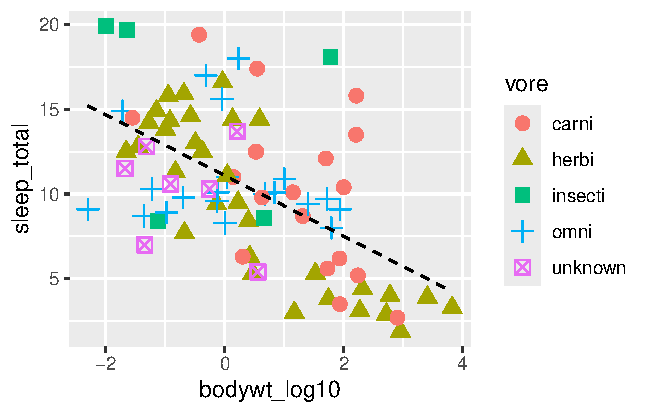
\includegraphics[scale = 0.75]{graphics/ch2Figs/ggEx_11.pdf}
\end{figure}

\noindent By setting \R{method = "lm"} on line 4, we are instructing \textit{ggplot2} to draw a linear model. While the concepts of standard error, polynomial regression, and linear models are more advanced topics, their value in displaying trends should be clear enough, even if the underlying mathematics is not yet fully understood.


It is at this point where the versatility of the \textit{ggplot2} really begins to shine.  For instance, if we wanted to create a separate regression line for each category of \R{\$vore} we can accomplish that by once again making use of the \R{aes()} function and ``grouping'' by \R{\$vore}.

\begin{inR}
ggplot(msleep, aes(x = bodywt_log10, y = sleep_total)) +
  geom_point(size = 3, aes(colour = vore, shape = vore)) +
  geom_smooth(
    method = "lm",
    se = FALSE,
    colour = "black",
    linewidth = 0.5,
    aes(group = vore)
  )
\end{inR}

%\vspace{2em}

\begin{figure}[H]
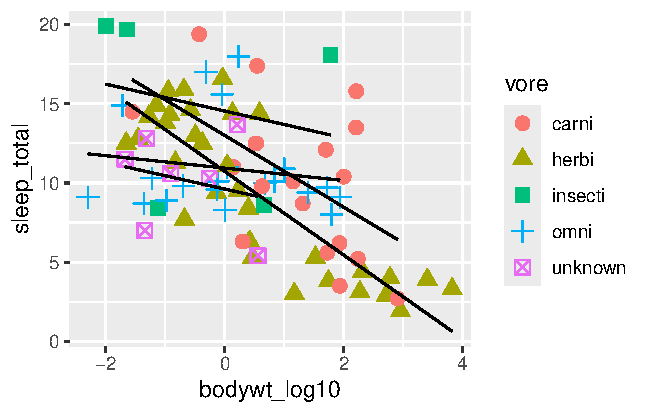
\includegraphics[scale = 0.75]{graphics/ch2Figs/ggEx_12.pdf}
\end{figure}

At present it is not clear which line applies to which category, but we could also have each regression line correspond to the colour mapped to \R{\$vore}, and (in consideration of colour blindness) give each line a separate \R{linetype}.

\begin{inR}
ggplot(msleep, aes(x = bodywt_log10, y = sleep_total)) +
  geom_point(size = 3, aes(colour = vore, shape = vore)) +
  geom_smooth(
    method = "lm",
    se = FALSE,
    linewidth = 0.5,
    aes(colour = vore, linetype = vore)
    )
\end{inR}

\vspace{2em}

\begin{figure}[H]
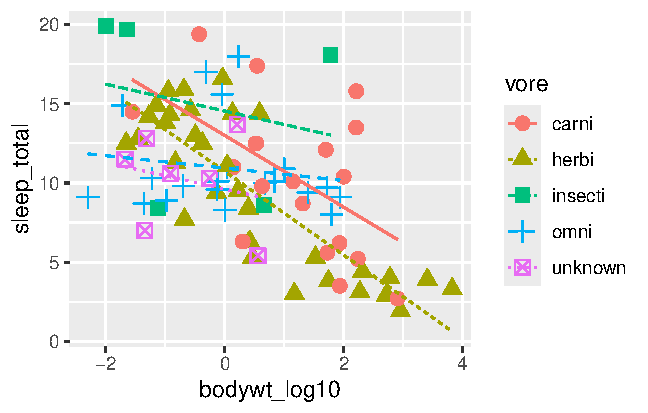
\includegraphics[scale = 0.75]{graphics/ch2Figs/ggEx_13.pdf}
\end{figure}

\section{Facets}
\label{sec:facets}

As interesting as our plot looks, it is becoming rather cluttered and difficult to visually parse. In situations like this, it is often helpful to split the plot up into separate facets (i.e., give each category its own graph). \textit{ggplot2} makes this very easy with its \R{facet\_wrap()} function.

\begin{inR}
ggplot(msleep, aes(x = bodywt_log10, y = sleep_total)) +
  geom_point(size = 3, aes(colour = vore, shape = vore)) +
  geom_smooth(
    method = "lm", 
    se = FALSE,
    linewidth = 0.5,
    aes(colour = vore)
  ) +
    facet_wrap(~ vore)
\end{inR}
\vspace{2em}
\begin{figure}[H]
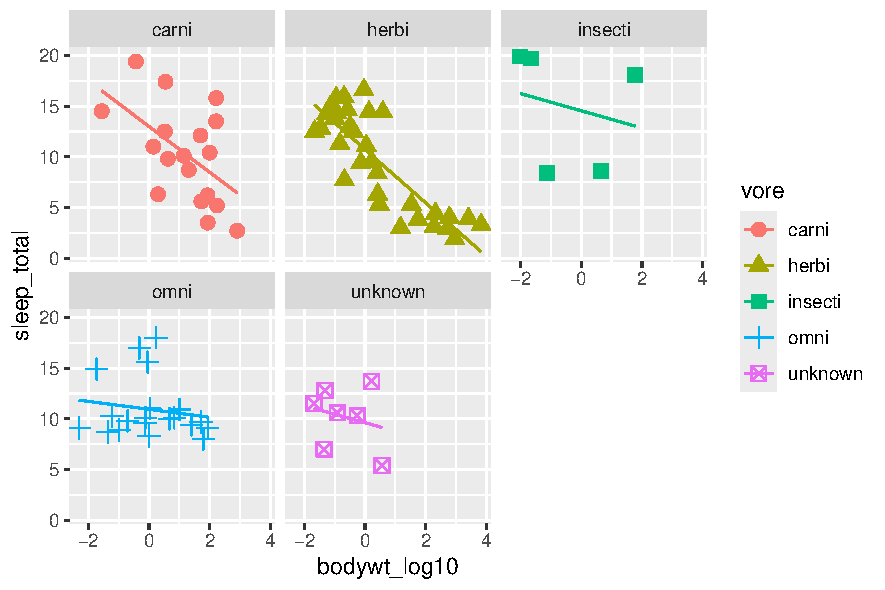
\includegraphics[scale = 0.75]{graphics/ch2Figs/ggEx_14.pdf}
\end{figure}

You can interpret the small formula we wrote (\R{\textasciitilde vore}) as meaning ``\textit{plot as a function of vore}.''

Notice that now, the colour and shape aesthetics are providing redundant information with the facet labels. As a general rule, you want to avoid redundancy in your plots because additional visual elements might bias the viewer's eye in unpredictable ways. We can easily fix this by removing some of the aesthetics we added earlier, and we can also adjust the facets so that they are all on a single row by adding the argument, \R{nrow = 1} to our \R{facet\_wrap()} function.

\begin{inR}
ggplot(msleep, aes(x = bodywt_log10, y = sleep_total)) +
  geom_point(size = 3) +
  geom_smooth(method = "lm", se = FALSE, linewidth = 0.5) +
  facet_wrap(~ vore, nrow = 1)
\end{inR}

\vspace{2em}

\begin{figure}[H]
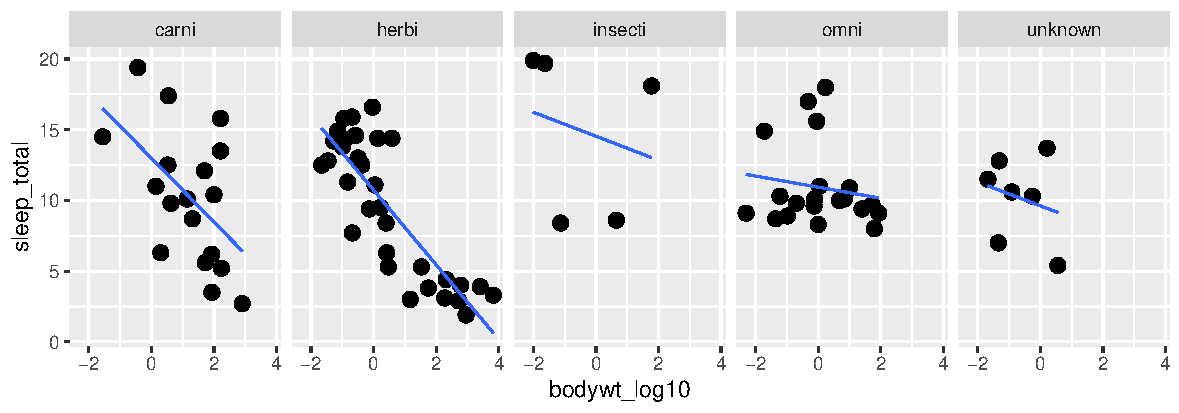
\includegraphics[scale = .75]{graphics/ch2Figs/ggEx_15.pdf}
\end{figure}

The default behaviour of \R{facet\_wrap()} preserves the x and y axis scales across the facets, making them easy to compare. In most cases, this is a feature you do not want to override but it can be done (see the R documentation: \R{?facet\_wrap}).

Particularly for beginners with R, it is difficult to impress how useful \textit{ggplot2} is here. Using base R plotting functions to produce a comparable graph would be a considerably more complex process and require a heftier amount of code to be written, whereas ggplot does it all for us in four short lines.

To finish up the plot, we should adjust some of the labelling, save it, and then take a look at some other more advanced features of \textit{ggplot2}.

\clearpage
\section{Labels}

To adjust the x and y axis titles we can simply use the functions \R{xlab()} and \R{ylab()}.

\begin{inR}
ggplot(msleep, aes(x = bodywt_log10, y = sleep_total)) +
  geom_point(size = 3) +
  geom_smooth(
    method = "lm",
    se = FALSE,
    linewidth = 0.5
  ) +
  facet_wrap(~vore, nrow = 1) +
  xlab("Log10(Body Weight kg)") + 
  ylab("Sleep Total (hrs)")
\end{inR}

\vspace{2em}

\begin{figure}[H]
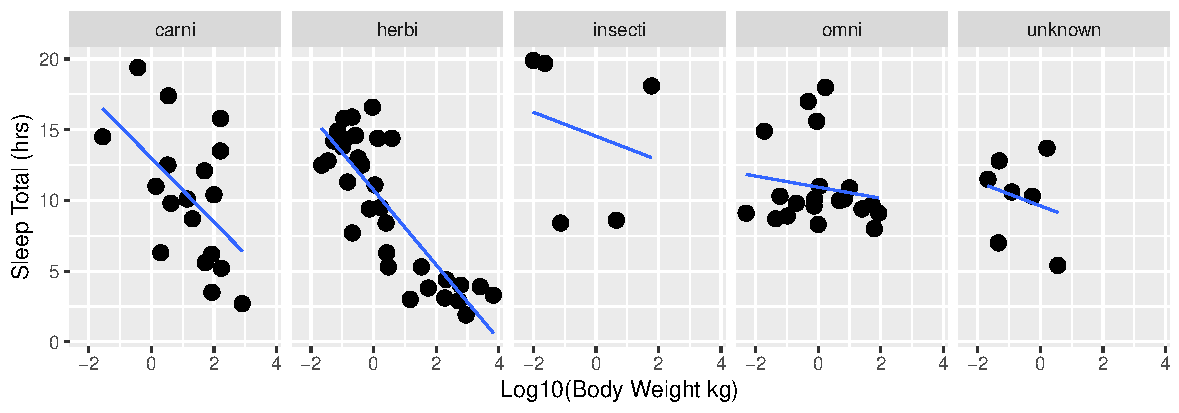
\includegraphics[scale = .75]{graphics/ch2Figs/ggEx_16.pdf}
\end{figure}

\section{Saving the plot}

Users of R studio will notice that in the \textit{Plots} pane there is a button that can be used to ``export'' your plot. However, it is usually more efficient and useful to save the plot via written code, and there are different methods you could use to go about this.  Since we are using \textit{ggplot2} to create our graphs, the optimal strategy is to use the \R{ggsave()} function, which will save the last generated plot unless you tell it otherwise.

\begin{inR}
ggsave("msleep_plot.png", dpi = 300, units = "cm", width = 20, height = 7)
\end{inR}
\vspace{1em}

Running this code as is will save the plot to your \textit{working directory} (see section \ref{sec:dir} for more info about directories and saving files). Within the function, we have chosen to name our image file \R{"msleep\_plot.png"}. The file extension you specify at the end of the file name here will dictate what type of image the plot is saved as.  In this case, it will save as a .PNG (Portable Network Graphics) image file, which is a very standard type of image that most people and software are used to handling, though you could save it as other common formats as well (e.g., .JPG, .GIF, .TIFF, etc.). The argument \R{dpi} stands for ``dots per inch'' and specifies the resolution of the image. For publication quality plots it is generally recommended that you have a minimum resolution of 300 dpi.  Anything less than that will likely produce very noticeable artifacting or fuzziness, particularly if the image has been resized or magnified. The last three arguments \R{units}, \R{width} and \R{height} allow you to specify the dimensions of your plot and should be relatively self-explanatory. If you wanted to, for instance, give the dimensions of your plot in millimeters you would specify \R{"mm"}, inches would be \R{"in"}, and so on.

\subsection{Vector graphics vs. Raster graphics}

The above code saved the plot as a .PNG which is a type of ``raster'' image, meaning it is an image composed of tiny coloured squares called pixels. The more pixels an image has, the more detail it can provide (i.e., the higher its resolution). The problem with using raster images though, is that resizing, stretching, and magnification has deleterious effects on their quality.  For instance, the image below shows a small section of our 300 dpi graph magnified substantially.

\vspace{1em}

\begin{figure}[H]
\centering

\includegraphics[scale = .3]{graphics/ch2Figs/artifacting_1.png}
\caption{Artificating present on our 300 dpi raster image when magnified.}
\end{figure}

A close inspection reveals jaggedness on the blue line and general blurriness around the rest of the image's elements. In academic publications, manuscripts, and presentations, this is something you want to avoid because, while these problems may not be immediately noticeable at first glance, they can impact a person's sensation of the image and, by extension, their opinion of its creator. Moreover, imperfections like these can be exacerbated in the printing and publishing process.

Now you might think that a simple remedy would be to increase the dpi to a much higher value, but this is generally a strategy you want to avoid.  There tends to be diminishing returns with resolution increases and anything beyond 300 dpi is not going to do much for you apart from ballooning the image's file size. The optimal strategy is to make use of something called a vector graphic.

Vector graphics are not really images in the traditional sense; rather, they are more akin to a set of instructions your computer uses to draw the image. Consequently, a vector-based image can be resized and magnified as much as you would like and it will never lose its quality. The drawback to vector graphics is that they do not work too well for highly detailed photographs (e.g., a forested landscape) and they are not always recognized by software. For instance, the most common types of vector you will encounter are .PDF, .SVG, and .EPS.  Recent versions of Microsoft Word and PowerPoint will happily accommodate .SVG files, but if you are wanting to use a .PDF or .EPS, you will be out of luck. Correspondingly, Google Docs and Google Slides will not accept any type of vector graphic, which is doubly frustrating because these apps will also downscale the resolution of raster graphics you import. Libre Office's Writer and Impress applications will accept a .PDF image, but it converts it to a lower resolution raster graphic when it is imported. Despite these types of compatibility limitations, if you are able to use vector graphics then you should, because they will give your work a level polish other people are not likely to have.

To save a file as a vector graphic, the process is the same as before, we just need to modify the file extension and remove the \R{dpi} argument (because dpi has no meaning for vector graphics).

\begin{inR}
ggsave("msleep_plot.svg", units = "cm", width = 20, height = 7)
\end{inR}

\vspace{1em}

The above code saved the image as a .SVG (Scalable Vector Graphic) file. This is a commonly used image file in web design, meaning it will, by default, be most likely displayed within a web-browser when you open it.

\begin{figure}[H]
\centering
\includesvg[scale = .3]{graphics/ch2Figs/artifacting_2.svg}
\caption{Magnification of a vector graphic.}
\end{figure}


\section{Scales}

A core concept in the ``grammar'' of \textit{ggplot2} is that of scales. Scales control how data is mapped to different aesthetics. For instance, there are scales for position, colour, size, shape, linetype, and so on. When you map an aesthetic to a variable like we did above where we had mapped both colour and shape to the \R{\$vore} column - e.g.,

\begin{inR}
...
geom_point(aes(colour = vore, shape = vore))
...
\end{inR}

\vspace{2em}

\begin{figure}[H]
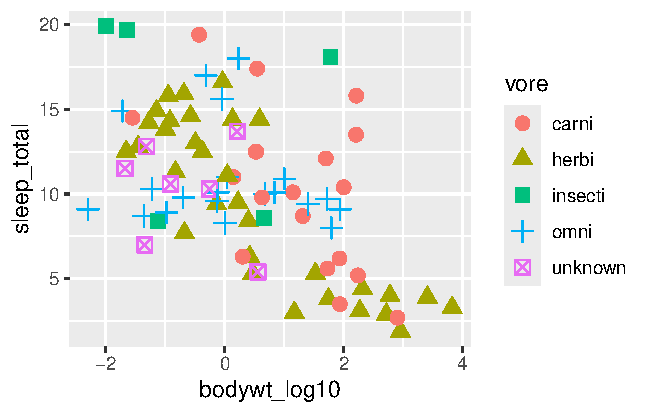
\includegraphics[scale = 0.75]{graphics/ch2Figs/ggEx_9.pdf}
\end{figure}

\vspace{1em}

\noindent
\textit{ggplot2} automatically chose which colours and shapes got applied to each category, but you can use functions to override these automatic mappings. 

The function you use to make these overrides is going to be dictated by the aesthetic you want to modify. For instance, to adjust the colour (or edge colour) of a point you could use the \R{scale\_\textbf{colour}\_discrete()} function or the \R{scale\_\textbf{colour}\_continuous()} function. If you wanted to adjust the shapes of the points, you could use \R{scale\_\textbf{shape}\_discrete()} function.  If you wanted to adjust the fill colour of something (e.g., the fill colour of points or the fill colour of bars on a graph), you could use \R{scale\_\textbf{fill}\_discrete()} function or the \R{scale\_\textbf{fill}\_continuous()} function.

There are a large amount of functions like these and, at this point, you do not need to concern yourself with all their varieties and how they work. What is important to recognize here is that each scale function specifies, inside its name, what aesthetic (e.g., colour, shape, fill, etc.) it is modifying:

\begin{center}
    \R{scale\_\textit{<aesthetic name>}\_\textit{<transformation>}()}
\end{center}

The ``transformation'' part of the function's name is intended to describe how the function modifies the aesthetic which will hopefully become more apparent as we move through some examples.

\subsection{Position Scales: Modifying the Axis Breaks}
\label{sec:pos_scale}

When we first created the grid on to which we drew our points, we had actually mapped some aesthetics to do this. Specifically, we mapped the x and y aesthetics to the \R{\$bodywt} and \R{\$sleep\_total} columns respectively. In other words, we had written:

\begin{inR}
ggplot(data = msleep, aes(x = bodywt, y = sleep_total))
\end{inR}

\vspace{1em}

When first mapping the x and y axes of a plot, \textit{ggplot2} typically selects an appropriate sequence of values to display for each. These are what are referred to as axis \textit{breaks} and, most of the time, \textit{ggplot2}'s default scaling for the breaks is excellent. However, there are occasions where more customized scaling is necessary. In these situations, the following four functions are useful:

\begin{enumerate}
\setlength\itemsep{-1em}
    \item \R{scale\_x\_continuous()}
    \item \R{scale\_y\_continuous()}
    \item \R{scale\_x\_discrete()}
    \item \R{scale\_y\_discrete()}
\end{enumerate}

\noindent
The above four functions allow you to easily modify what values appear on your axis; though, which one you use depends on whether your axis has a \textit{continuous} or \textit{discrete} \gls{position scale}. Position scales control the location mappings of a plots visual elements.

In the case of the mammal sleep data we plotted, both the x-axis scale (body weight) and y-axis scale (sleep total) are \textit{continuous} in nature. In other words, the axis values represent measured numeric values as opposed to categories. Another way of conceptualizing this continuous vs discrete distinction is to approach it from R's perspective. In this case, both axes represent \textit{numeric} objects as opposed to \textit{character} objects. Thus, for the purpose of plotting, they are treated as a continuous scale.

\begin{inR}
mode(msleep$bodywt_log10) # x-axis
mode(msleep$sleep_total) # y-axis
\end{inR}
\begin{outR}
[1] "numeric"
[1] "numeric"
\end{outR}

If we had, for instance, plotted a categorical variable on the x-axis (e.g., the conservation status of the animal) then the x-axis would be discrete while the y-axis remains continuous (we will see an example of this later on).

To customize the breaks on our axis, we simply need to add one of the aforementioned functions to our plot's code and provide a vector of values we want to see displayed using the argument \R{breaks}. For instance, if we want the x-axis to only display the numbers 1, 2, and 3, we would add \\ \R{scale\_x\_continuous(breaks = c(1,2,3))} to our code (see line 11).

\begin{inR}
ggplot(msleep, aes(x = bodywt_log10, y = sleep_total)) +
  geom_point(size = 3) +
  geom_smooth(
    method = "lm",
    se = FALSE,
    linewidth = 0.5
  ) +
  facet_wrap(~vore, nrow = 1) +
  xlab("Log10(Body Weight kg)") + 
  ylab("Sleep Total (hrs)") + 
  scale_x_continuous(breaks = c(1,2,3))
\end{inR}

\vspace{2em}

\begin{figure}[H]
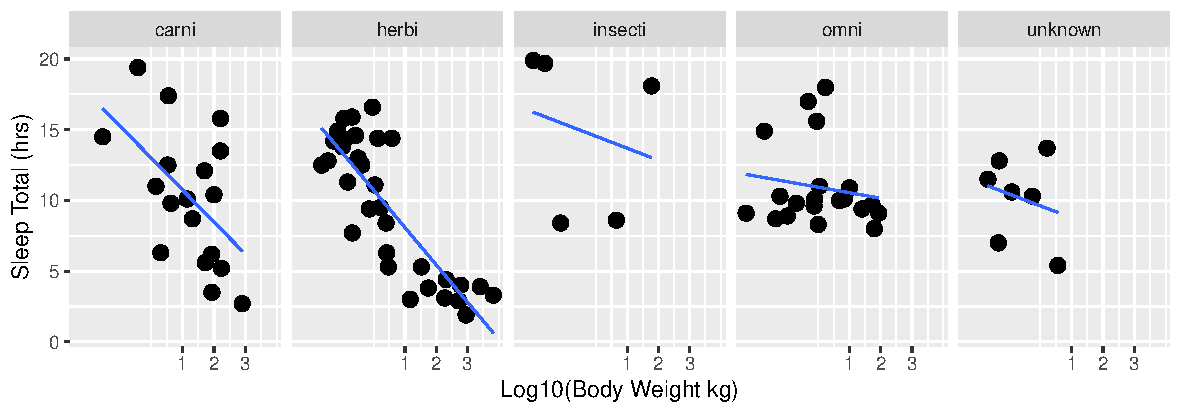
\includegraphics[scale = .75]{graphics/ch2Figs/ggEx_17.pdf}
\end{figure}

In general, the best practice is not to specify values individually, but rather specify a sequence using the \R{seq()} function we learned about in Chapter 1 (see section \ref{sec:func_args}). For instance, we could have the x-axis increment by 1s and the y-axis increment by 2s (see lines 11 and 12).

\begin{inR}
ggplot(msleep, aes(x = bodywt_log10, y = sleep_total)) +
  geom_point(size = 3) +
  geom_smooth(
    method = "lm",
    se = FALSE,
    linewidth = 0.5
  ) +
  facet_wrap(~vore, nrow = 1) +
  xlab("Log10(Body Weight kg)") + 
  ylab("Sleep Total (hrs)") + 
  scale_x_continuous(breaks = seq(-2, 4, 1)) +
  scale_y_continuous(breaks = seq(0, 20, 2))
\end{inR}

\vspace{2em}

\begin{figure}[H]
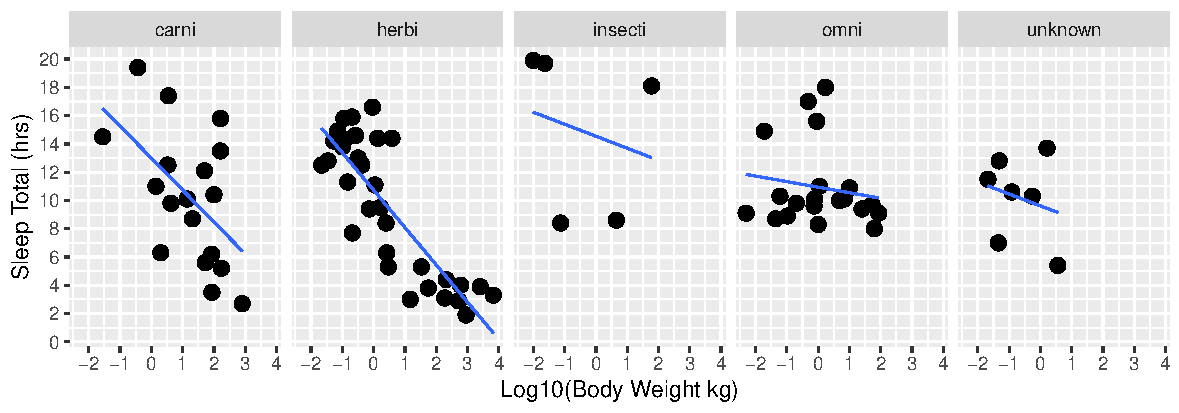
\includegraphics[scale = .75]{graphics/ch2Figs/ggEx_18.pdf}
\end{figure}

The four scale functions above can achieve a lot more than what is being shown here, but for most uses, this basic adjustment of the axis breaks will be their primary purpose.

\subsection{Modifying the Axis Range}

In addition to axis break adjustment, the range of the axis will often require customization as well.  To achieve this, the best practice is usually to use the function \R{coord\_cartesian()}.  To illustrate with some absurd values, we could have the x-axis span between -2 and +1 and have the y-axis span between $-5$ and $+10$.

\begin{inR}
ggplot(msleep, aes(x = bodywt_log10, y = sleep_total)) +
  geom_point(size = 3) +
  geom_smooth(
    method = "lm",
    se = FALSE,
    linewidth = 0.5
  ) +
  facet_wrap(~vore, nrow = 1) +
  xlab("Log10(Body Weight kg)") + 
  ylab("Sleep Total (hrs)") +
  scale_x_continuous(breaks = seq(-2, 4, 1)) +
  scale_y_continuous(breaks = seq(0, 20, 2)) +
  coord_cartesian(xlim = c(-2, 1), ylim = c(-5, 10))
\end{inR}

\vspace{2em}

\begin{figure}[H]
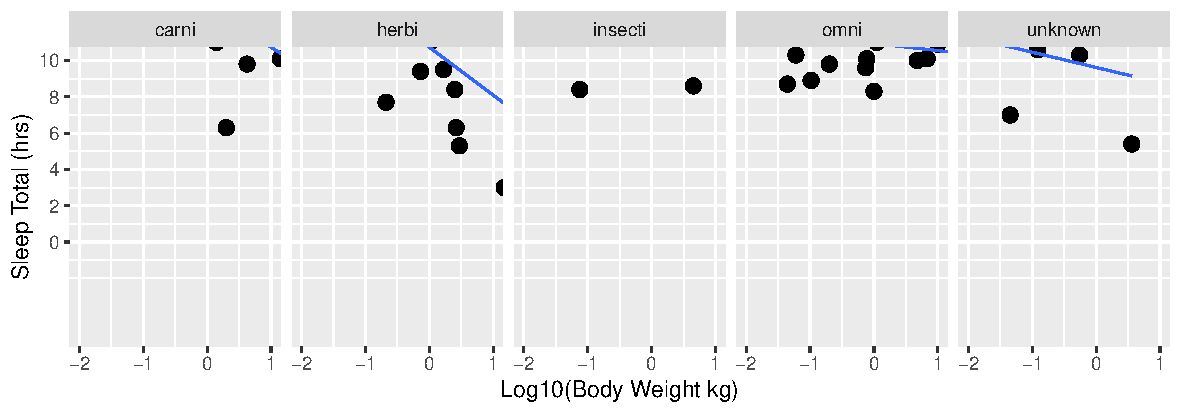
\includegraphics[scale = .75]{graphics/ch2Figs/ggEx_19.pdf}
\end{figure}

\noindent
Note that, while the y-axis goes as low as -5, it does not show breaks below 0 because of how the \R{breaks} argument in \R{scale\_y\_continuous()} were set.

At this point it is worth offering a disclaimer.  Within the position scale functions mentioned earlier (i.e., \R{scale\_x\_continuous()} and \R{scale\_y\_continuous()}, there is an argument called \R{limits} that will allow you to set the range of the scale in a manner similar to the \R{coord\_cartesian()} function. Additionally, \textit{ggplot2} also has two other functions, \R{xlim()} and \R{ylim()}, that will do the same. However, setting the limits of your plot with these arguments and functions is best avoided because they will remove data falling outside of those specified limits. This can result in problems if your plot's code is performing some type of statistical calculation. For instance, if you remove lines 12 and 13 in the above script and add \R{ylim(-2, 1)} you will be confronted with a very nasty error message, telling you (among other things) that ...

\begin{outR}
Warning messages:
1: Removed 83 rows containing non-finite outside the scale range
(`stat_smooth()`). 
\end{outR}

\noindent
This occurs because values in our data falling outside of $-2$ and $+1$ are not recognized anymore, but \textit{ggplot2} needed those values to calculate that blue regression line using the \R{geom\_smooth()} function. Thus, the moral of the story is, if you need to ``zoom-in'' or ``zoom-out'' on a plot, use \R{coord\_cartesian()}. Do not be tempted by those other options.\footnote{Readers are probably wondering ``\textit{what use does removing data outside of the limits serve? It seems like it would only ever cause more problems than it solves (especially if you are unaware it is happening).}'' And to that I say, yes.}

\subsection{Colour Scales: Modifying Colour Mappings}

Similar to how \textit{ggplot2} automatically selected a scaling for the breaks on the x and y axis, it also automatically selected various colours to use when we mapped colour to the \R{$vore$} column. Moreover, the distinction between \textit{continuous} and \textit{discrete} scaling applies just as much to colour as it does position. As illustrated in Figure \ref{fig:continuous_col_scale} and \ref{fig:discrete_col_scale}, discrete colour scales are usually represented with a colour gradient and discrete scales are represented by distinct colours (like in a box of crayons). While it is possible to do this, you usually do not want to use a gradient to represent distinct categories because it makes the categories difficult to discriminate visually. For instance, the \R{\$vore} column we mapped to the colour aesthetic earlier contained distinct non-numeric categories (e.g., carni, herbi, insecti, and so on); thus, a colour palette such as that seen in Figure \ref{fig:discrete_col_scale} would be much more appropriate than Figure \ref{fig:continuous_col_scale}.

\vspace{2em}

\begin{figure}[h]
\centering

\includegraphics[scale = .4]{graphics/ch2Figs/col_gradient.pdf}
\caption{Example of a continuous colour scale (i.e., a colour gradient).}
\label{fig:continuous_col_scale}
\end{figure}

\vspace{2em}

\begin{figure}[H]
\centering

\includegraphics[scale = .4]{graphics/ch2Figs/col_discrete.pdf}
\caption{Example of a discrete colour scale (a.k.a. a qualitative palette.)}
\label{fig:discrete_col_scale}
\end{figure}

\vspace{1em}

\subsection{Discrete Colour Scales}
\label{sec:discrete_cols}

To illustrate the use of discrete colour scales lets create a simple plot we can experiment with.

\begin{inR}
ggplot(msleep, aes(x = bodywt_log10, y = sleep_total)) +
  geom_point(size = 3, shape = 21, stroke = 2)
\end{inR}

\vspace{2em}

\begin{figure}[H]
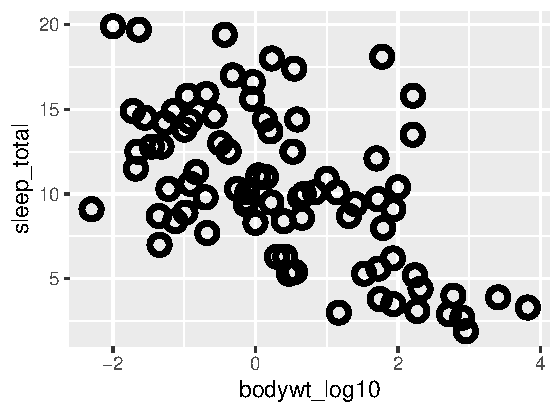
\includegraphics[scale = .75]{graphics/ch2Figs/ggEx_20.pdf}
\end{figure}

\noindent
First we will map the edge colour to the column \R{\$vore}.

\begin{inR}
ggplot(msleep, aes(x = bodywt_log10, y = sleep_total)) +
  geom_point(
    size = 3, shape = 21, stroke = 2,
    aes(colour = vore)
  )
\end{inR}

\vspace{2em}

\begin{figure}[H]
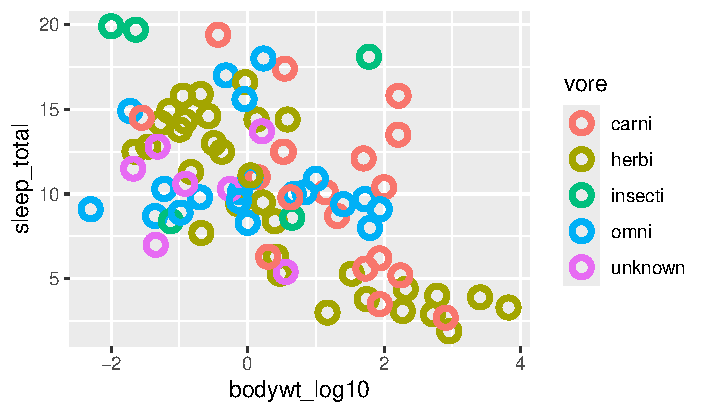
\includegraphics[scale = .75]{graphics/ch2Figs/ggEx_21.pdf}
\end{figure}

\noindent
Then, to override these colours we can simply use \R{scale\_colour\_discrete()} and input a vector of colours.

\begin{inR}
ggplot(msleep, aes(x = bodywt_log10, y = sleep_total)) +
  geom_point(
    size = 3, shape = 21, stroke = 2,
    aes(colour = vore)
  ) +
  scale_colour_discrete(type = c("red", "blue", "green", "purple", "orange"))
\end{inR}

\vspace{2em}

\begin{figure}[H]
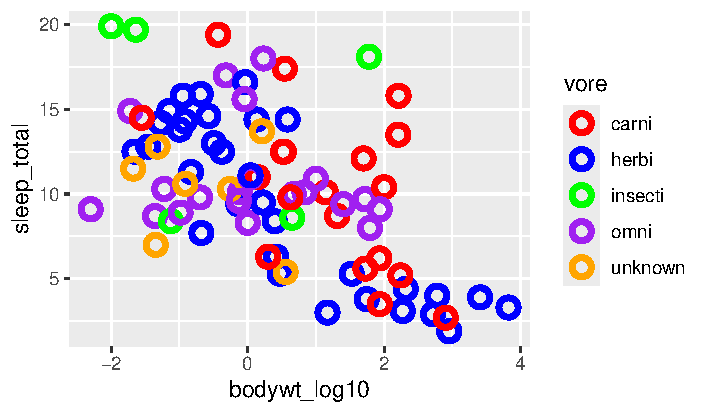
\includegraphics[scale = .75]{graphics/ch2Figs/ggEx_22.pdf}
\end{figure}

The same effect can be achieved by using \R{scale\_colour\_manual()} instead.

\begin{inR}
...
scale_colour_manual(values = c("red", "blue", "green", "purple", "orange"))
\end{inR}

\vspace{1em}

\noindent
However, the advantage to using \R{scale\_colour\_discrete()} is you are not limited by the number of categories in your palette. This means you can create a bigger colour palette and \textit{ggplot2} will only use as many colours as needed. By contrast, if you use \R{scale\_colour\_manual()}, you have to ensure that you specify the same amount of colours as there are categories. To illustrate, we can create a palette with eight colours, but \textit{ggplot2} will only use the first six.

\begin{inR}
# Create a colour palette
palette <- c(
  "#000000", "#DF536B", "#61D04F", "#2297E6", "#28E2E5", "#CD0BBC", "#F5C710",
  "#9E9E9E"
)

# Use that palette in your plot
ggplot(msleep, aes(x = bodywt_log10, y = sleep_total)) +
  geom_point(
    size = 3, shape = 21, stroke = 2,
    aes(colour = vore)
  ) +
  scale_colour_discrete(type = palette)
\end{inR}

\vspace{2em}

\begin{figure}[H]
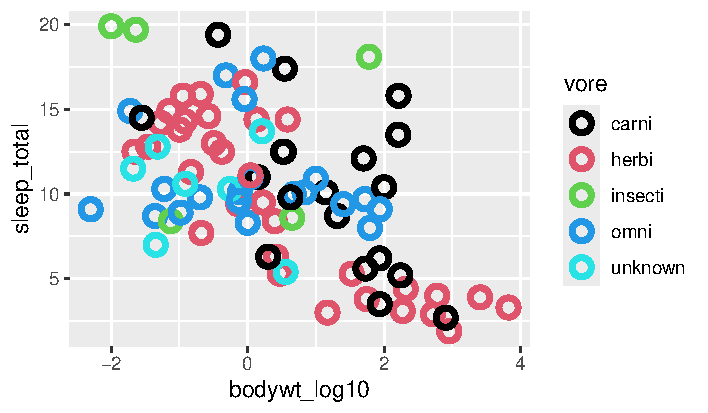
\includegraphics[scale = .75]{graphics/ch2Figs/ggEx_23.pdf}
\end{figure}


Notice that we are using pch 21 as our shape. Recall that this shape takes both an edge and fill colour (see Figure \ref{fig:points.pdf}). At present, we have not specified a fill colour, so the points are hollow. However, instead of modifying the edge colour like we have been doing, we could modify the fill colour of the points and just keep the edges black.

\begin{inR}
ggplot(msleep, aes(x = bodywt_log10, y = sleep_total)) +
  geom_point(
    size = 3, shape = 21, stroke = 1, colour = "black",
    aes(fill = vore)
  ) +
  scale_fill_discrete(type = palette)
\end{inR}

\vspace{2em}

\begin{figure}[H]
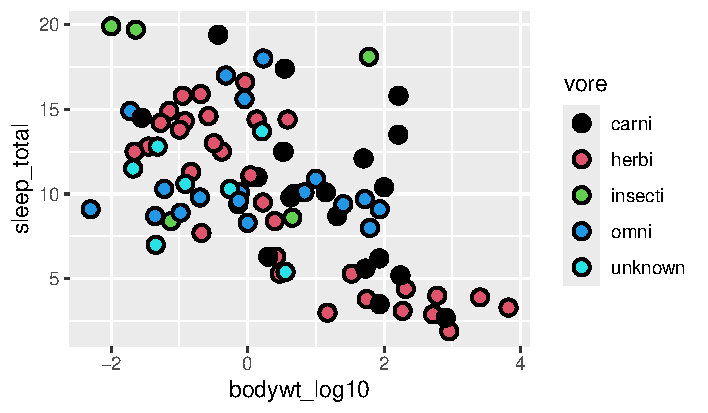
\includegraphics[scale = .75]{graphics/ch2Figs/ggEx_24.pdf}
\end{figure}

\noindent
Notice where the important changes have taken place in the code.  We have moved the \R{colour} aesthetic outside of the \R{aes()} function.  This means a single \R{colour} (black) will now be mapped to all the points. We have also mapped the \R{\$vore} column to the \R{fill} aesthetic inside of \R{aes()} and, for that reason, now specify \R{scale\_\textbf{fill}\_discrete()} to modify the colour options. In other words, we are now adjusting the \textit{fill} colour, not the point/edge colour.

\subsubsection{Pre-Existing Discrete Colour Palettes}

Until now, we have been specifying our own custom colour palettes; however, base R contains a variety of pre-existing palettes we can make use of. To obtain the list you can simply run the following:

\begin{inR}
palette.pals()
\end{inR}
\begin{outR}
 [1] "R3"              "R4"              "ggplot2"         "Okabe-Ito"      
 [5] "Accent"          "Dark 2"          "Paired"          "Pastel 1"       
 [9] "Pastel 2"        "Set 1"           "Set 2"           "Set 3"          
[13] "Tableau 10"      "Classic Tableau" "Polychrome 36"   "Alphabet"
\end{outR}

Of note, palettes \R{"R4"}, \R{"Okabe-Ito"}, \R{"Dark 2"}, \R{"Paired"}, and \R{"Set 2"}, are all decently robust under conditions of colour vision deficiency. To obtain a vector of the hex codes used for a specific palette, you can just run \R{palette.colors(n = NULL, "Dark 2")}, but it is usually more convenient to insert this function directly into \textit{ggplot2}. Figure \ref{fig:discrete_cols} illustrates the colours employed in each palette - only eight colours are shown but some do contain more.

\begin{inR}
ggplot(msleep, aes(x = bodywt_log10, y = sleep_total)) +
  geom_point(
    size = 3, shape = 21, stroke = 1, colour = "black",
    aes(fill = vore)
  ) +
  scale_fill_discrete(type = palette.colors(n = NULL, "Dark2"))
\end{inR}

\vspace{2em}

\begin{figure}[H]
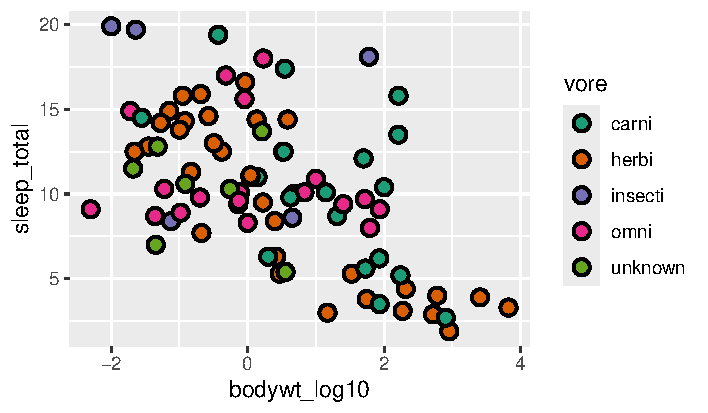
\includegraphics[scale = .75]{graphics/ch2Figs/ggEx_25.pdf}
\end{figure}

\vspace{2em}

\begin{figure}[p]
\centering
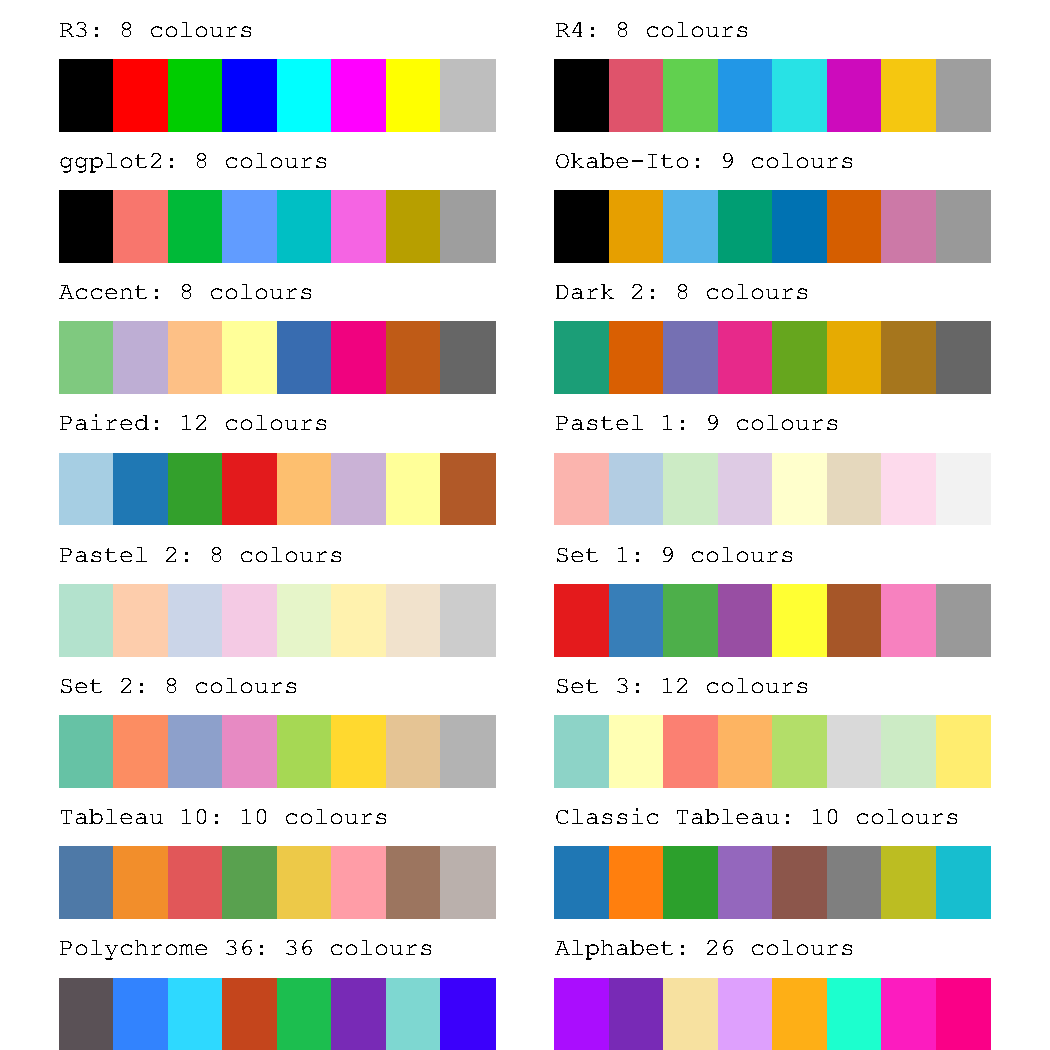
\includegraphics[width = \textwidth]{graphics/ch2Figs/palettes.pdf}
\caption{Examples of the various discrete colour palettes in base R.}
\label{fig:discrete_cols}
\end{figure}

\subsection{Continuous Colour Scales}

Continuous colour scales operate more or less in the same manner as discrete ones; however, to illustrate them, we need to map colour to a continuous variable. In the \R{msleep} data, there is a column called \R{\$brainwt} which, similar to \R{\$bodywt}, is a continuous measure. To visualize it adequately we will need to log transform it as well. For simplicity we will do this directly in the plot's code:

\clearpage

\begin{inR}
ggplot(msleep, aes(x = bodywt_log10, y = sleep_total)) +
  geom_point(
    size = 3, shape = 21, stroke = 1, colour = "black",
    aes(fill = log10(brainwt))
  )
\end{inR}

\vspace{2em}

\begin{figure}[H]
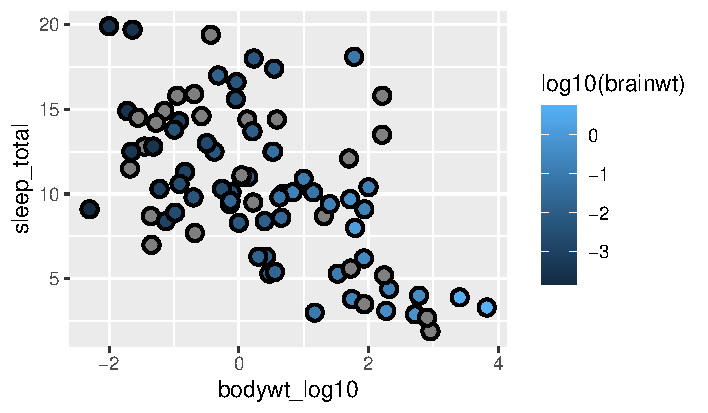
\includegraphics[scale = .75]{graphics/ch2Figs/ggEx_26.pdf}
\end{figure}

Immediately you can see we are now presented with a \textit{colourbar} instead of a set of fixed colours. This is because the nature of the variable \R{\$brainwt} is that it is continuous. Thus, it does not fall neatly into distinct categories.  Between any two brain weights there is a theoretically infinite amount of values and the colourbar's gradient offers a means of representing that. As you move from black to blue, lighter shades of blue are indicative of a heavier brain weight. Looking at the graph, increases in body weight also seem to correspond to increases in brain weight, but notice the grey points in the graph.  Those are indicative of missing values in the \R{\$brainwt} column and with a bit of R code, we can filter the data to see what values these are specifically.

\begin{inR}
filter(msleep, is.na(brainwt))
\end{inR}

\vspace{1em}

In case it is not obvious, this code works by using the \R{is.na()} function to check whether each row in the \R{msleep} data frame's  \R{\$brainwt} column contains an \R{NA} value. Rows which result as \R{TRUE} are displayed and everything else is ignored. This leaves us with a data frame of 27 different animals, all of which have a \R{NA} value in the \R{\$brainwt} column.


If you are left unsatisfied by the default black to blue gradient, \textit{ggplot2} makes it easy to produce custom colour gradients using the \R{scale\_fill\_gradient()} and \R{scale\_fill\_gradient2()} functions, and of course there are colour aesthetic variants of this for situations where you want to modify the edge and point colours.\footnote{These are \R{scale\_colour\_gradient()} and \R{scale\_colour\_gradient2()}.} Both functions simply require you to specify a \R{low} colour argument that represents the bottom of the colourbar and a \R{high} colour argument that represents the top of the colour bar. However, \R{scale\_colour\_gradient2()} also requires you to specify the argument \R{mid}, which indicates a third midpoint colour. You can even specify the location of this midpoint with the argument \R{midpoint}. More succinctly \R{scale\_colour\_gradient()} creates \textit{sequential} colour palettes, and \R{scale\_colour\_gradient2()} creates \textit{diverging} colour palettes.

In addition to those main arguments, you can also specify what colour you would like \R{NA} values to be represented by and set the the breaks that appear on the colourbar. These are given by the arguments \R{na.value} and \R{breaks} respectively.

\begin{inR}
# scale_colour_gradient example
ggplot(msleep, aes(x = bodywt_log10, y = sleep_total)) +
  geom_point(
    size = 3, shape = 21, stroke = 1, colour = "black",
    aes(fill = log10(brainwt))
  ) +
  scale_fill_gradient(
    low = "blue",
    high = "red",
    na.value = "green", 
    breaks = seq(-4, 1, 1)
  )
\end{inR}

\vspace{2em}

\begin{figure}[H]
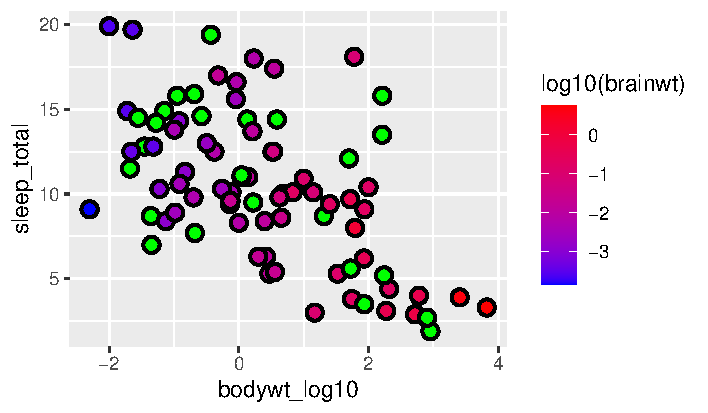
\includegraphics[scale = .75]{graphics/ch2Figs/ggEx_27.pdf}
\end{figure}

\clearpage

With the mammal sleep data, there is no logical reason to plot a midpoint colour using \\ \R{scale\_colour\_gradient2()} but to illustrate its use we will depict a midpoint using the colour \R{"grey"} and we will place it at a $\text{log}_{10}(\text{brain weight}) = -1.5$.

\begin{inR}
# scale_colour_gradient2 example
ggplot(msleep, aes(x = bodywt_log10, y = sleep_total)) +
  geom_point(
    size = 3, shape = 21, stroke = 1, colour = "black",
    aes(fill = log10(brainwt))
  ) +
  scale_fill_gradient2(
    low = "blue",
    mid = "grey",
    high = "red",
    midpoint = -1.5,
    na.value = "green", 
    breaks = seq(-4, 1, 1)
  )
\end{inR}

\vspace{2em}

\begin{figure}[H]
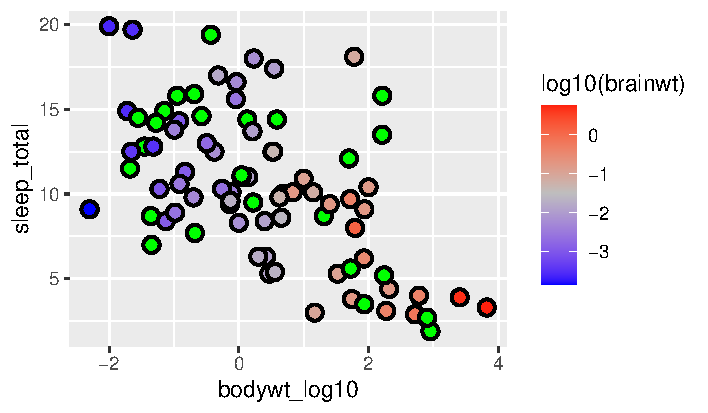
\includegraphics[scale = .75]{graphics/ch2Figs/ggEx_28.pdf}
\end{figure}

\subsubsection{Pre-Existing Continuous Colour Palettes}

Similar to what we saw with discrete colour scales, R comes with a set of continuous colour palettes we can use, some of which are sequential and some of which are diverging. For those interested, these palettes are based around an HCL (hue-chroma-luminance) colour space model which confers some advantages over the HSV (hue-saturation-value) colour space model computers have traditionally employed \parencite{Zeileis2019}.

To obtain a list of these HCL palettes you can simply run any of the following lines for sequential, diverging, and qualitative palettes respectively.

\begin{inR}
hcl.pals(type = "sequential")
hcl.pals(type = "diverging")
hcl.pals(type = "qualitative")
\end{inR}

\vspace{1em}

The qualitative palettes work best for discrete scales (i.e., identifying distinct categories) where you want each category to have equal perceptual weight. These are not much use for our present purposes but are notable because they are based on a HCL colour space model. That means we are not limited by the amount of colours in the palette like we were with R's standard discrete colour palettes (see section \ref{sec:discrete_cols}). Though, anecdotally, when you go beyond 6 categories the HCL qualitative palettes' colours start to become more and more difficult to discriminate between (even with standard colour vision). Interestingly, \textit{ggplot2}'s default discrete colour selection relies on a similar underlying theory.

To obtain the hex codes for any given palette (e.g., \R{"Inferno"}) you will, in addition to providing the palette name, need to specify how many hex codes you want to see using the argument \R{n}. Visual examples of the three HCL palette types are provided in Appendix \ref{sec:AppendixPalettes}.

\begin{inR}
hcl.colors(n = 8, palette = "Inferno") 
\end{inR}
\begin{outR}
[1] "#040404" "#341348" "#701069" "#AB1E75" "#DC4962" "#F58426" "#F8C149" "#FFFE9E"
\end{outR}

To use one of base R's HCL colour palettes in our plot we can use the function \\ \R{scale\_fill\_gradientn()} to set our palette. The function just takes a vector of colours and extrapolates a gradient from that.

\begin{inR}
ggplot(msleep, aes(x = bodywt_log10, y = sleep_total)) +
  geom_point(
    size = 3, shape = 21, stroke = 1, colour = "black",
    aes(fill = log10(brainwt))
  ) +
  scale_fill_gradientn(
    colours = hcl.colors(n = 50, palette = "Inferno"),
    na.value = "grey", 
    breaks = seq(-4, 1, 1)
  )
\end{inR}

\vspace{2em}

\begin{figure}[H]
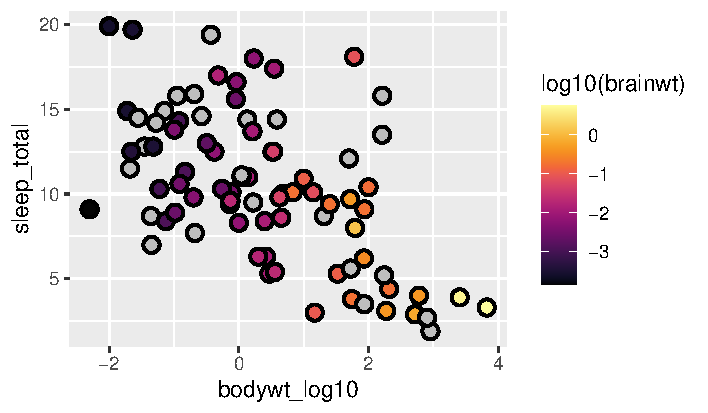
\includegraphics[scale = .75]{graphics/ch2Figs/ggEx_29.pdf}
\end{figure}

\subsection{Shape Scales}

We know that relying solely on colour to visually discriminate categories is inadvisable due to colour vision deficiencies people may have; thus, in addition to adjusting the colour scales, we can also adjust the shape scale simultaneously by mapping \R{\$vore} to both \R{shape} and \R{fill} within the \R{aes()} function. For the shapes we will use the pch symbols 21 - 24 and also have the category ``unknown'' be represented by pch 13 (see Figure \ref{fig:points.pdf}) - recall that these particular symbols (21 - 24) take both a colour and fill aesthetic. We will keep the edges (i.e., colour aesthetic) black but, for the fill aesthetic, we will use the \R{"R4"} colour palette (see Figure \ref{fig:discrete_cols}).

\begin{inR}
ggplot(msleep, aes(x = bodywt_log10, y = sleep_total)) +
  geom_point(
    size = 3, stroke = 1, colour = "black",
    aes(fill = vore, shape = vore)
  ) +
  scale_shape_manual(values = c(21:24), na.value = 13) +
  scale_fill_discrete(type = palette.colors(n = NULL, "R4"))
\end{inR}

\vspace{2em}

\begin{figure}[H]
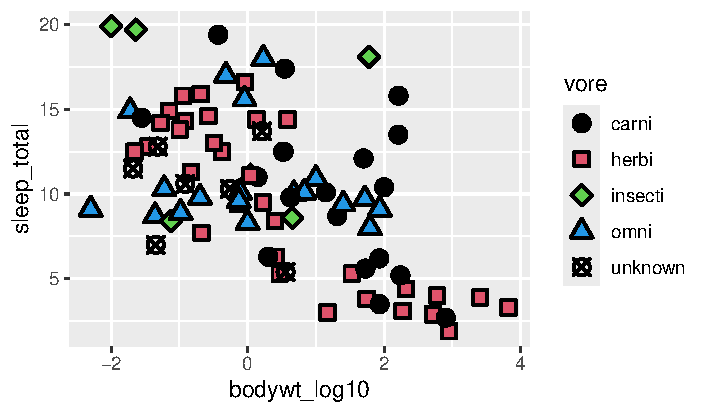
\includegraphics[scale = .75]{graphics/ch2Figs/ggEx_30.pdf}
\end{figure}

\subsection{Legend Titles}

In all the examples above, the legend that \textit{ggplot2} produced has always been titled with the name of the column it is representing. For instance, when we mapped the categories in the \R{\$vore} column it was titled ``vore.'' When we mapped \R{log10(brainwt}, it was titled ``log10(brainwt).'' To adjust the name of the legend, each \R{scale} function we have used also takes a \R{name} argument which will dictate how the legend is titled. For instance, keeping with the above example, we could adjust the legend title to read "Diet".

\begin{inR}
ggplot(msleep, aes(x = bodywt_log10, y = sleep_total)) +
  geom_point(
    size = 3, stroke = 1, colour = "black",
    aes(fill = vore, shape = vore)
  ) +
  scale_shape_manual(values = c(21:24), na.value = 13, name = "Diet") +
  scale_fill_discrete(type = palette.colors(n = NULL, "R4"), name = "Diet")
\end{inR}

\vspace{2em}

\begin{figure}[H]
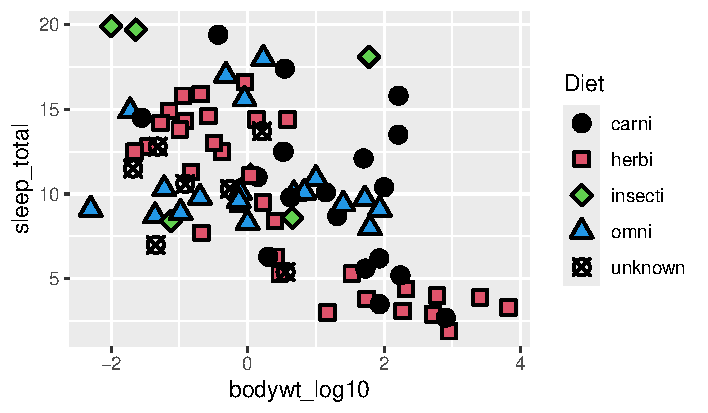
\includegraphics[scale = .75]{graphics/ch2Figs/ggEx_31.pdf}
\end{figure}

In this example, we have two scales in our legend, the \R{shape} scale and the \R{fill} scale.  If you do not specify an identical name for each, they will be treated as separate legends. For instance, try giving \R{scale\_shape\_manual()} a different name than \R{scale\_fill\_discrete()} and see what happens.

An alternative method for renaming your legend is to add the function \R{labs()} to your plot's code and specify the name of each scale as a separate argument.

\begin{inR}
ggplot(msleep, aes(x = bodywt_log10, y = sleep_total)) +
  geom_point(
    size = 3, stroke = 1, colour = "black",
    aes(fill = vore, shape = vore)
  ) +
  scale_shape_manual(values = c(21:24), na.value = 13) +
  scale_fill_discrete(type = palette.colors(n = NULL, "R4")) +
  labs(
    shape = "Diet",
    fill = "Diet"
  )
\end{inR}

\vspace{1em}

\subsection{Other Scales}

In the sections above, we have only considered the position, colour, fill, and shape scales, which are among the features most frequently appealed to when graphing, but similar functions exist for other scales. For instance, there are scale functions to modify the size, linewidth, and linetype aesthetics if needed. To learn more about these and other features, an excellent resource is the tidyverse's official \textit{ggplot2} website, which contains a learning section that will direct you to various excellent resources (\url{https://ggplot2.tidyverse.org/}), the best and most comprehensive of which is the official manual for \textit{ggplot2} titled ``ggplot2: Elegant Graphics for Data Analysis.'' Keeping with the ethos of ``free software'', this is available to read online for free at 

\begin{center}
\url{https://ggplot2-book.org/}
\end{center}

\section{Modifying Other Non-data Components}

One thing that will be apparent is that \textit{ggplot2} has a very specific ``look'' to it, and that look is not arbitrary. It was crafted meticulously on the basis of expert advice. In the language of \textit{ggplot2}, this look is what is referred to as a \textit{theme}.  Specifically, we are seeing \R{theme\_grey()} and in the dark master's own words:

\begin{displayquote}
\headingfont
%\large
The theme is designed to put the data forward while supporting comparisons, following the advice of Tufte \citeyear{Tufte2006}; Brewer \citeyear{Brewer1994}; Carr \citeyear{Carr2002}, \citeyear{Carr1994}; Carr and Sun \citeyear{Carr1999}. We can still see the gridlines to aid in the judgement of position \parencite{Cleveland1993}, but they have little visual impact and we can easily `tune' them out. The grey background gives the plot a similar typographic colour to the text, ensuring that the graphics fit in with the flow of a document without jumping out with a bright white background. Finally, the grey background creates a continuous field of colour which ensures that the plot is perceived as a single visual entity.

- \cite{Wickham_ggplot2}

\end{displayquote}

\noindent
To sum up, the grey theme is immaculate in its conception and cannot be improved upon. In fact, once one has borne witness to the majesty of \R{theme\_grey()}, even small departures from it can have drastic effects on a person's physical and mental well being. That being said, \textit{ggplot2} still offers its users the ability to modify any aspect of the plot they wish - just be careful what you wish for.

\subsection{Built-in Themes}

Once the scaling and other main visual elements related to data presentation are complete, it is often helpful to set your plot's code as a variable you can append other elements to. Meaning that, in the same way a number in R is an object that you can name and add things to - e.g., 

\begin{inR}
x <- 1
x + 2
\end{inR}
\begin{outR}
[1] 3
\end{outR}

\noindent
your plot is also an object (just a very complex one) that you can \textit{add} things to. For instance, on the first line of our plot's code, right before the function \R{ggplot()}, we could give our plot the name \R{my\_plot}.

\begin{inR}
my_plot <- ggplot(msleep, aes(x = bodywt_log10, y = sleep_total)) +
  geom_point(
    size = 3, colour = "black",
    aes(fill = vore, shape = vore)
  ) +
  scale_shape_manual(values = c(21:24, 13)) +
  scale_fill_discrete(type = palette.colors(n = NULL, "R4")) +
  labs(
    shape = "Diet",
    fill = "Diet"
  ) +
  xlab("Log10(Body Weight kg)") + ylab("Sleep Total (hrs)")
\end{inR}

\vspace{1em}

\noindent
Now, when you run \R{my\_plot} you can see it output to the plot window.

\begin{inR}
my_plot 
\end{inR}

\vspace{2em}

\begin{figure}[H]
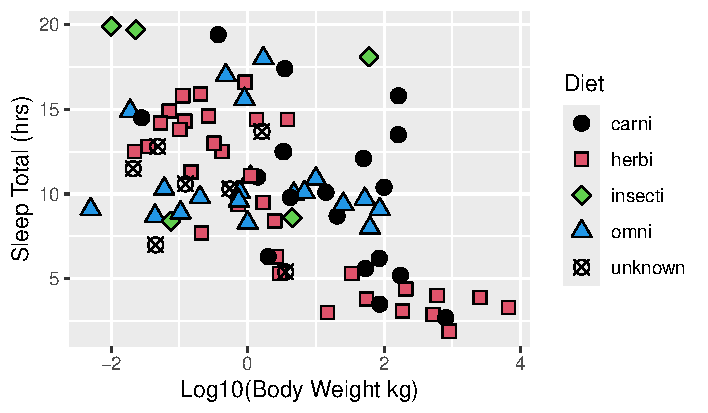
\includegraphics[scale = .75]{graphics/ch2Figs/ggEx_32.pdf}
\end{figure}

The quickest way to modify the overall appearance of your plot - which works well as a starting point for other modifications you want to make - is to use one of ggplot2's built in themes shown in Figure \ref{fig:gg_built-in-themes}.  Simply add the theme's function to your plot's code.  For instance, if you wanted to use the black and white theme, \R{theme\_bw()}, you would run ...

\begin{inR}
my_plot + theme_bw()
\end{inR}

\vspace{1em}

\noindent
Additional pre-built themes can be accessed via other R packages, such as \R{ggthemes}.

\vspace{2em}

\begin{figure}[p]
\centering
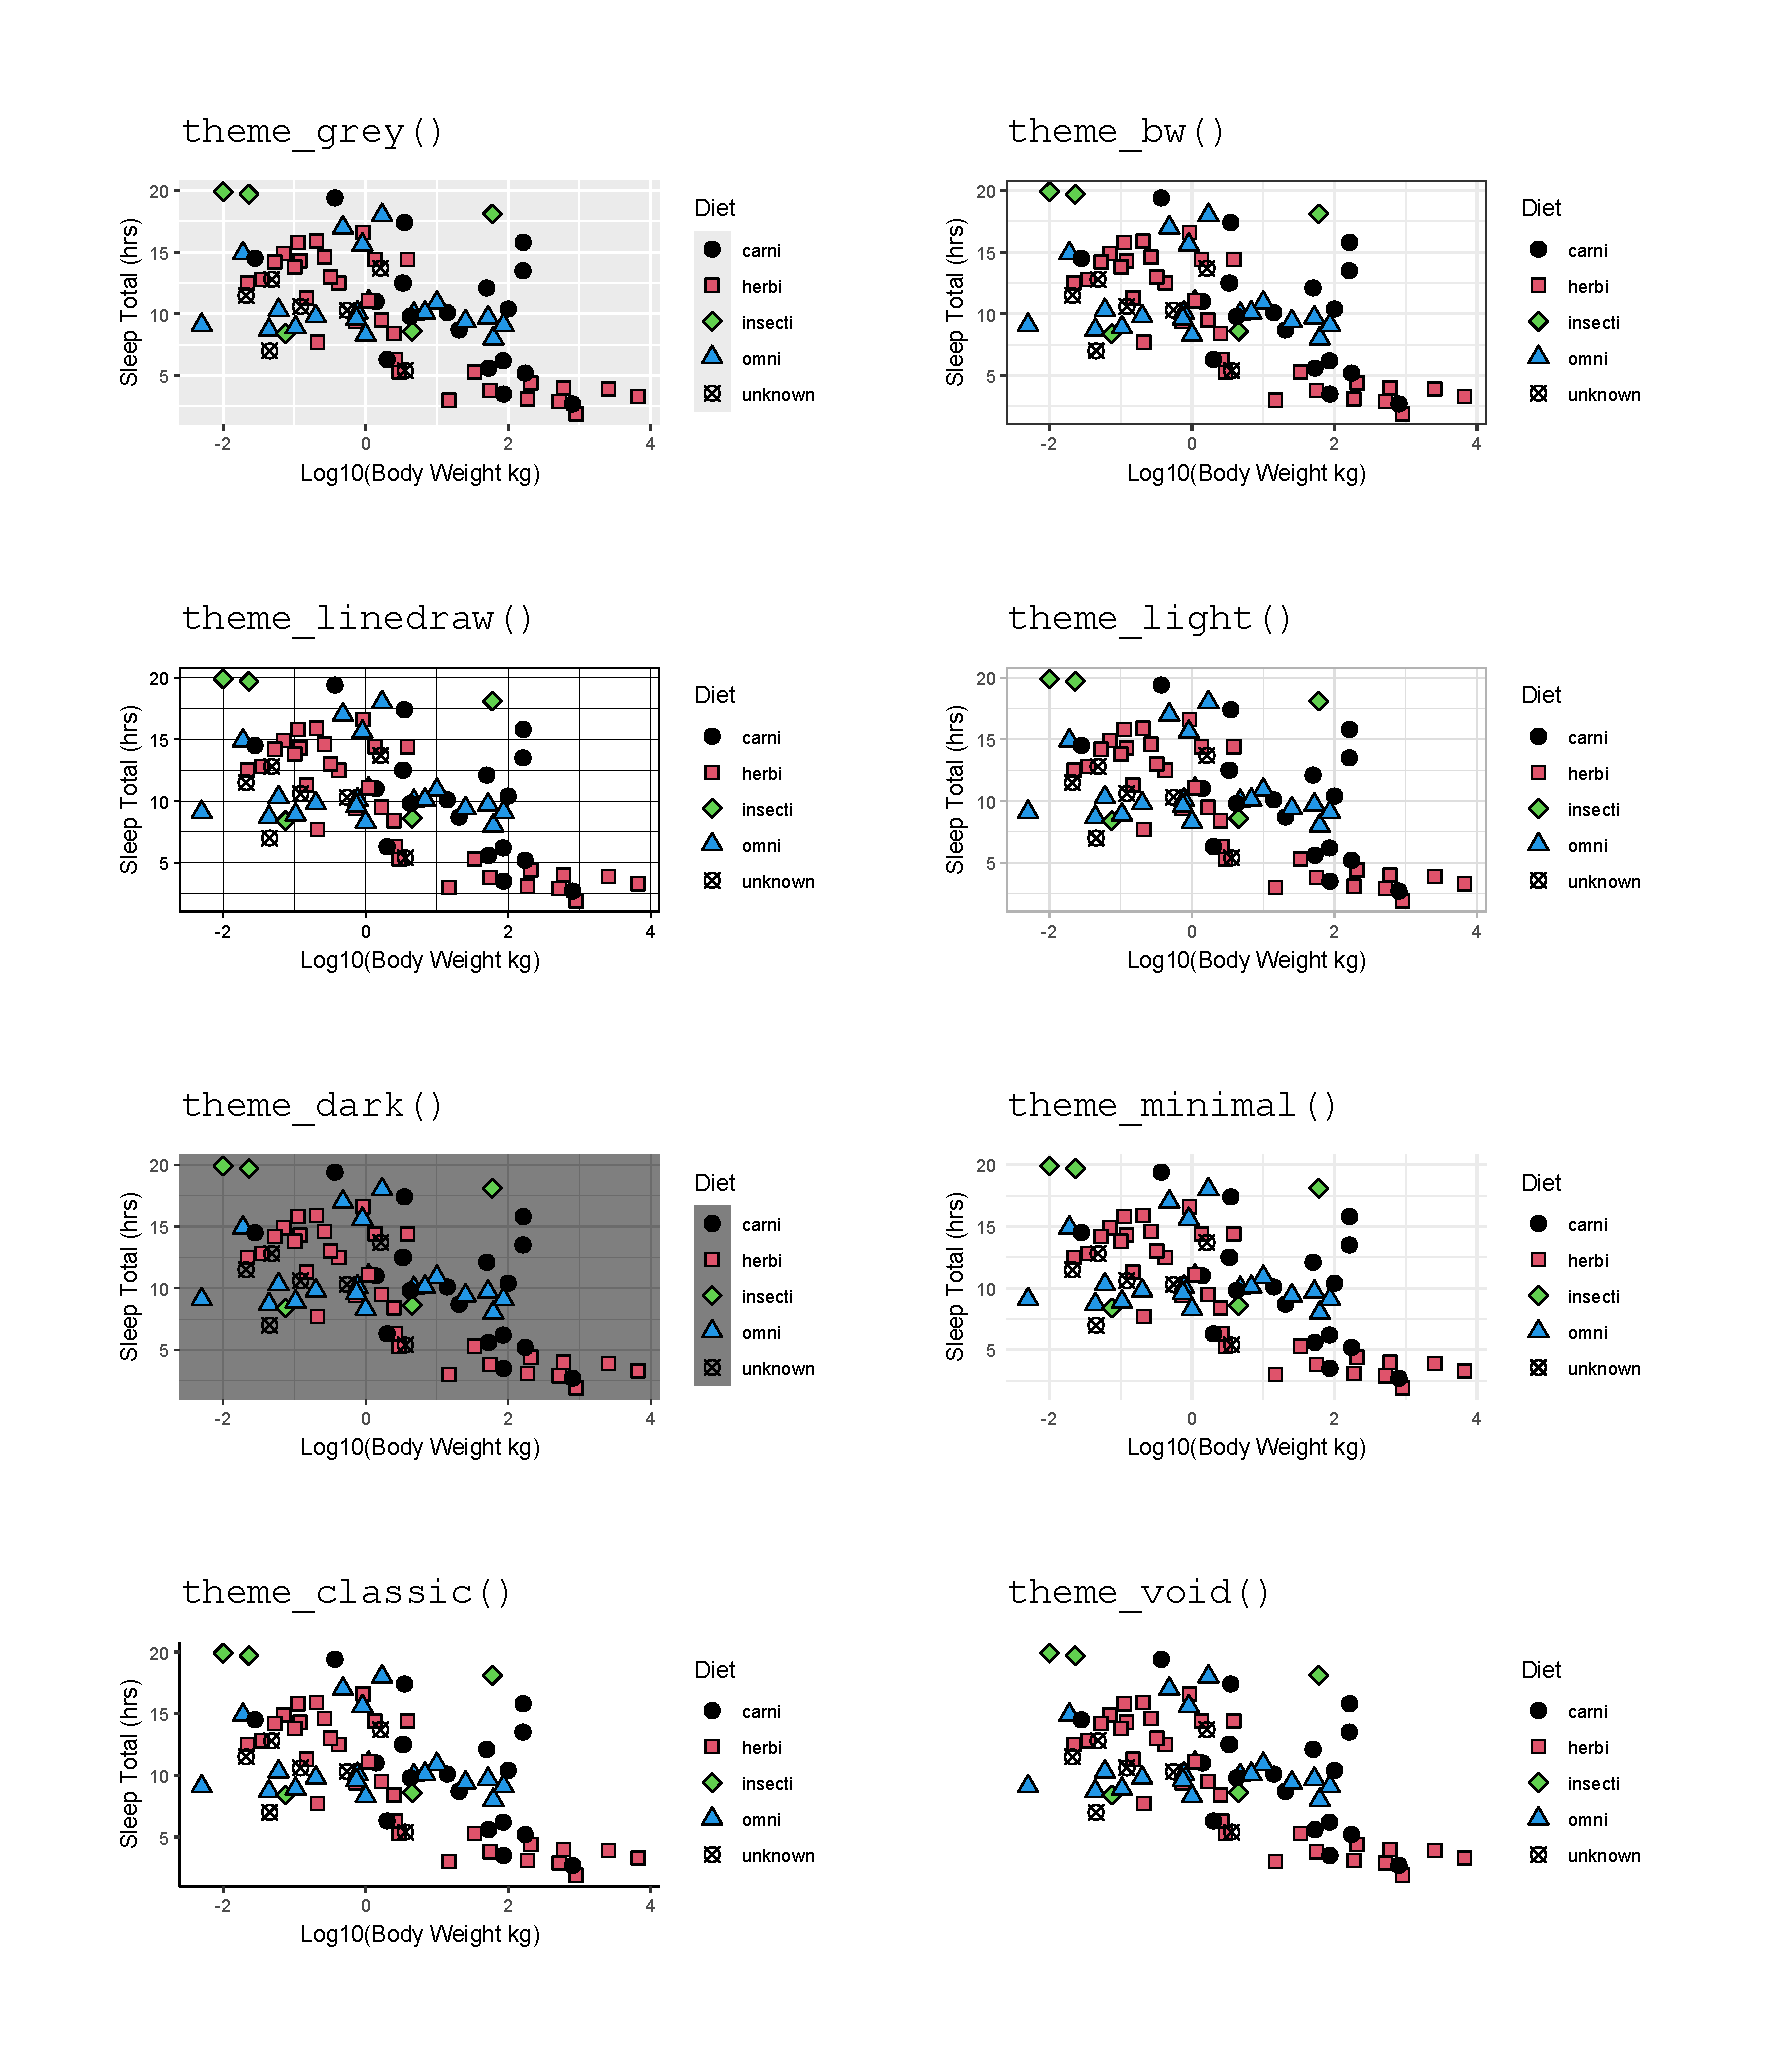
\includegraphics[width = \textwidth]{graphics/ch2Figs/ggEx_themes.pdf}
\caption{Visual examples of the eight built-in themes \textit{ggplot2} provides.}
\label{fig:gg_built-in-themes}
\end{figure}

\vspace{1em}

\subsection{Customizing Themes}

Obtaining a more fine-grained control over the visual elements will require the use of \textit{ggplot2}'s \R{theme()} function. Admittedly, there is so much customization possible here that an exhaustive explanation would require at least an additional chapter's worth of content. For simplicity, we will restrict the discussion to axis text modifications. This should illustrate the overall process well-enough and generalize nicely across the plot's numerous other elements. That being said, readers looking to adjust these other elements will still need consult documentation of some kind for specifics. The official \textit{ggplot2} manual is unquestionably the best resource in this respect:

\begin{center}
\url{https://ggplot2-book.org/themes.html#sec-theme-elements}
\end{center}

To modify the axis text, we first need to specify, within the \R{theme()} function, the name of the element we want to modify. In this case, since we want to modify \textit{both} the x and y axis, we will specify \R{axis.text}.  Then we need to specify a function to modify this element we have chosen. In this case, since we want to modify text, we will use the function \R{element\_text()}. Within that, we can specify numerous arguments related to the text. For a full list of arguments, it is highly recommended that the reader consult the R documentation: \R{?element\_text()}

\begin{inR}
my_plot + theme_bw() +
  theme(
    axis.text = element_text(size = 18, face = "bold", colour = "red", angle = 45)
  )
\end{inR}

\vspace{2em}

\begin{figure}[H]
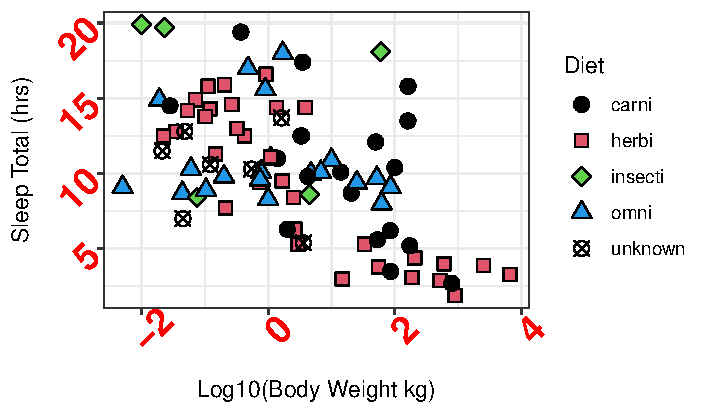
\includegraphics[scale = .75]{graphics/ch2Figs/ggEx_33.pdf}
\end{figure}

Notice that the code affected both axes; however, if we want to affect a change for only one axis (e.g., the x-axis) we just specify the element as \R{axis.text.x}.  This will also allow us to include a \R{margin} argument to affect the spacing around the text.

\begin{inR}
my_plot + theme_bw() +
  theme(
    axis.text.x = element_text(
      size = 18, face = "bold", colour = "red", angle = 45,
      margin = margin(t = 1, r = 0, b = 0, l = 0, unit = "cm")
    )
  )
\end{inR}

\vspace{2em}

\begin{figure}[H]
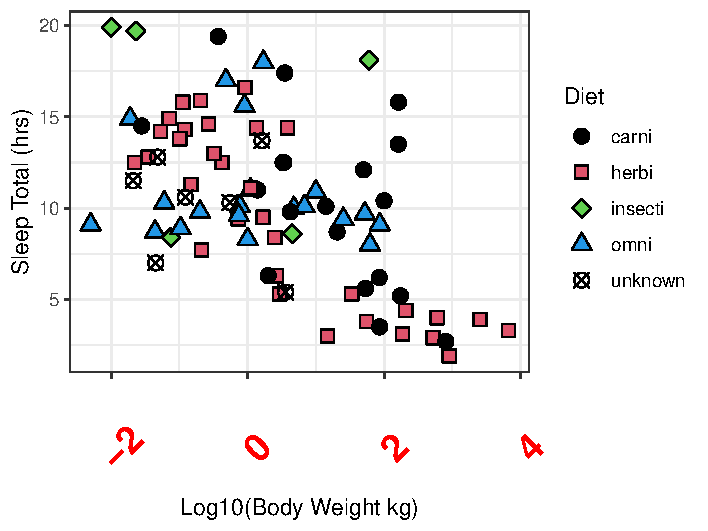
\includegraphics[scale = .75]{graphics/ch2Figs/ggEx_34.pdf}
\end{figure}

\clearpage

A similar logic applies to the axis title.  In that case we would modify the \R{axis.title} element. And again, if we wanted to modify the x-axis title specifically, we would use \R{axis.title.x}.  The y-axis title would of course be \R{axis.title.y}.

\begin{inR}
my_plot + theme_bw() +
  theme(
    axis.text.x = element_text(
      size = 18, face = "bold", colour = "red", angle = 45,
      margin = margin(t = 1, r = 0, b = 0, l = 0, unit = "cm")
    ),
    axis.title.y = element_text(
      size = 18, face = "italic", colour = "deepskyblue3", angle = 90
    )
  )
\end{inR}

\vspace{2em}

\begin{figure}[H]
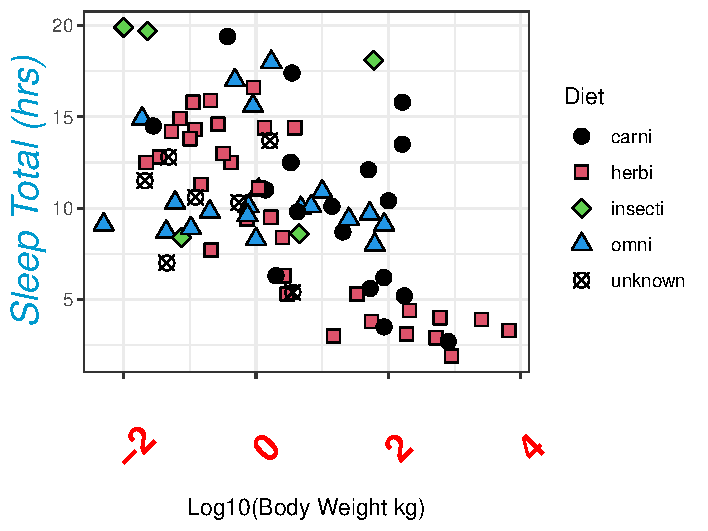
\includegraphics[scale = .75]{graphics/ch2Figs/ggEx_35.pdf}
\end{figure}

\clearpage

\section{A Final Note}

In the plots created above, we have gone through how to adjust a wide variety of elements but there are two adjustments that have not been discussed:

\begin{enumerate}
    \item How do you change the order of the categories?  For instance, suppose we wanted ``herbi'' to be at the top of the ``Diet'' legend. Or suppose we wanted it to come first in our sequence of faceted plots we created in section \ref{sec:facets}. How can we make that happen?
    \item  How do we adjust the names of the categories? Each category of vore/diet has had its name shortened, but what if we wanted to write out each category in its entirety. E.g., display ``carnivore'' instead of ``carni'', and ``herbivore'' instead of ``herbi'', and so on.
\end{enumerate}

The answer to both these questions requires first understanding ``factors,'' which will be explained later in the next chapter.
%\chapter{The Basics of Loading and Manipulating Data}
\chapter{The Invocation and Metamorphosis of Data}

\IMFellEnglish
\lettrine[lines=5, realheight]{K}{NOWLEDGE} is power as they say, but data—data is something else entirely. It is the ghost in the machine, the thing lurking beneath the surface, waiting for you to look too close. Heed this warning: The data frame, and its accursed successor the tibble, are your most loyal servants \ldots{} and your most treacherous foes. Treat them with reverence, for a single misstep may awaken errors best left entombed.

\normalfont

Chapter 1 had stated that \glspl{data frame} are essential for keeping a host of related information stored in a well organized manner that is easy to manipulate. When printed to the console, data frames present information in a familiar spreadsheet-like structure that can be created, subset, and altered in various ways (see section \ref{sec:data_frames} for details). Moreover, in chapter 1, we saw how a data frame can be constructed by manually entering values with R code. And, for all but the smallest of data sets, this method, while simple, is both time-consuming and highly prone to error. A better strategy is to take an existing file of information and import that directly into R as a data frame or, depending on the nature of the data and what needs to be done with it, as a list, matrix, array, or table. Though, a data frame is usually going to be the optimal choice and will be the primary focus of this chapter.

Data can come in all manner of different layouts and file formats and, in this respect, R has the ability to handle pretty much any scenario that might arise. This chapter will be working under the assumption that the kind of data that you need to work with is in a conventional ``spreadsheet-style'' of format. That is to say, like the \R{msleep} data used in Chapter 2, there are sets of rows and columns, with each cell containing just a single value.

\section{Spreadsheet Software}
\label{sec:spreadsheet_soft}

Given the ubiquity of spreadsheet software, it is important to discuss its use and why R offers a preferable alternative for data analysis. Most spreadsheet applications have their own specific file type that is tailored to its unique purpose and platform. For instance, \textit{Microsoft's Excel} spreadsheet application has its own proprietary format called the \texttt{.xlsx} file format. The awful stock spreadsheet application on Macintosh computers, called \textit{Numbers}, uses the \texttt{.NUMBERS} file format. And if you use an open-source spreadsheet software like \textit{Libre Office's Calc} application, you may be familiar with the \texttt{.ods} file format.

As everyone who is reading this doubtlessly appreciates, spreadsheet applications like Microsoft's Excel, Numbers, Libre Office's Calc, etc., do more than just structure your data in a big table.  They allow you to do things like perform calculations, adjust cell colours, add images, insert comments, etc. And all of this is saved, in one form or another, as information inside the specific file associated with that software. These features make applications like Microsoft's Excel, for instance, a great tool for basic tasks like balancing the household budget.  However, for serious data analysis that requires the use of large data sets and complex or heavy calculations, this kind of software is going to be more of a hindrance than a help. Incorporating all those layers of additional functionality is going to boost file sizes, inflate load times, limit the amount of information the spreadsheet can hold, and increase the chance of a glitch occurring. Additionally, and most importantly, both the analyses and the data are all contained within the same file, which makes it very easy to irrevocably damage your original data set, often without even realizing it. The fact is, we should care about analysing our data efficiently and safely, not making it look pretty in what amounts to a fancy table, and this is one of the key benefits of using R.

From the point of view of R, a spreadsheet is just a way of displaying the raw information to be analysed and nothing more. The analysis of that information is what R does. Technically then, we should not be referring to something as a ``spreadsheet file,'' but rather a ``data file.'' The spreadsheet aspect of all of this is more about how the data is structured for our viewing as humans. However, data does not necessarily need to be viewed as a spreadsheet - it can be viewed in all kinds of different ways. It is just that a spreadsheet is usually the most convenient and intuitive way to view it and talk about it.

\section{Using an Ethical File Format}
\label{sec:ethical_file}

As noted above, there are a variety of different spreadsheet file types data could be formatted as (\texttt{.xlsx}, \texttt{.ods}, \texttt{.wks}, etc.). To remain consistent with open-science principles \parencite{UNESCO_open_sci}, best practice dictates that you work with your data in a file format that is both universally recognized across applications and will also stand the test of time in terms of compatibility.  In other words, we want to (ideally) work with a file format that has no immediate risk of becoming obsolete and can be read by multiple computers on multiple platforms without forcing the user to pay for some proprietary application. Along these lines, the most widely used and recognized format is the \texttt{.csv} file format.

\section{The .CSV Format}

``CSV'' stands for ``comma separated values.'' It gets its name from the fact that it is, quite literally, nothing more than a generic text document that uses commas to denote a tabular (spreadsheet) structure in the data.\footnote{``Tabular'' and ``spreadsheet'' mean the same thing here.} This is easiest to see with an example. The GitHub repository for this book contains a file called \R{skull\_cap\_partial\_wide.csv}. It is located in the \R{./data} directory at the following URL:

\begin{center}
\url{https://github.com/statistical-grimoire/book/blob/main/data/Egyptian-skulls}
\end{center}

\noindent
This data represents a subset of a much larger dataset,\footnote{\R{Thomson\_Randall-MacIver\_1905.csv}} containing estimated cranial capacities in cubic centimetres for 1,449 ancient Egyptian skulls.\footnote{This is not necessarily a statistic anyone should care about, but Ancient Egypt is really cool and skulls are metal AF. Also, for any Americans reading this, 1 centimetre is equal to 1.181 barleycorns.} These skulls span numerous historical periods, ranging from Egypt's early predynastic era to its Roman occupation.

Upon opening the file on GitHub, the contents appear in a standard tabular format, resembling a typical spreadsheet (see Table \ref{tab:skulls_wide} for an example displaying the first ten rows). With the exception of the columns labelled \R{sex} and \R{predynastic}, each column header corresponds to the starting year of an approximate date range, as reported by the original authors. The prefix \textit{c} denotes \textit{circa} (meaning ``approximately''), followed by a year and the abbreviation \textit{BC} (``Before Christ''), reflecting the historical dating conventions employed by the original authors. A more contemporary and inclusive alternative would be \textit{BCE} (``Before Common Era''). The term \textit{predynastic} refers to periods preceding the earliest recorded Egyptian dynasties, which, at the time of \citeauthor{Thomson1905}'s (\citeyear{Thomson1905}) research, were not yet clearly established or reliably dated.

\vspace{1em}

\begin{table}[!h]
\centering
\resizebox{\textwidth}{!}{
\begin{tabular}{lrrrrrrrrrr}
\toprule
sex & predynastic & c4800BC & c4200BC & c4000BC & c3500BC & c2780BC & c1590BC & c378BC & c331BC & c3700BC\\
\midrule
\cellcolor{gray!10}{Male} & \cellcolor{gray!10}{1370} & \cellcolor{gray!10}{1410} & \cellcolor{gray!10}{1320} & \cellcolor{gray!10}{1445} & \cellcolor{gray!10}{1395} & \cellcolor{gray!10}{1425} & \cellcolor{gray!10}{1440} & \cellcolor{gray!10}{1310} & \cellcolor{gray!10}{1450} & \cellcolor{gray!10}{NA}\\
Male & 1250 & 1445 & 1565 & 1540 & 1420 & 1505 & 1355 & 1395 & 1460 & NA\\
\cellcolor{gray!10}{Male} & \cellcolor{gray!10}{1430} & \cellcolor{gray!10}{1440} & \cellcolor{gray!10}{1600} & \cellcolor{gray!10}{1565} & \cellcolor{gray!10}{1380} & \cellcolor{gray!10}{1360} & \cellcolor{gray!10}{1490} & \cellcolor{gray!10}{1360} & \cellcolor{gray!10}{1360} & \cellcolor{gray!10}{NA}\\
Male & 1350 & 1340 & 1460 & 1710 & 1260 & 1385 & 1425 & 1485 & 1410 & NA\\
\cellcolor{gray!10}{Male} & \cellcolor{gray!10}{1130} & \cellcolor{gray!10}{1460} & \cellcolor{gray!10}{1520} & \cellcolor{gray!10}{1690} & \cellcolor{gray!10}{1285} & \cellcolor{gray!10}{1350} & \cellcolor{gray!10}{1380} & \cellcolor{gray!10}{1365} & \cellcolor{gray!10}{1215} & \cellcolor{gray!10}{NA}\\
\addlinespace
Male & 1670 & 1290 & 1440 & 1775 & 1505 & 1440 & 1490 & 1220 & 1320 & NA\\
\cellcolor{gray!10}{Male} & \cellcolor{gray!10}{1195} & \cellcolor{gray!10}{1290} & \cellcolor{gray!10}{1740} & \cellcolor{gray!10}{1390} & \cellcolor{gray!10}{1230} & \cellcolor{gray!10}{1400} & \cellcolor{gray!10}{1385} & \cellcolor{gray!10}{1195} & \cellcolor{gray!10}{1550} & \cellcolor{gray!10}{NA}\\
Male & 1500 & 1385 & 1410 & 1620 & 1250 & 1255 & 1270 & 1410 & 1320 & NA\\
\cellcolor{gray!10}{Male} & \cellcolor{gray!10}{1325} & \cellcolor{gray!10}{1290} & \cellcolor{gray!10}{1510} & \cellcolor{gray!10}{1500} & \cellcolor{gray!10}{1315} & \cellcolor{gray!10}{1450} & \cellcolor{gray!10}{1585} & \cellcolor{gray!10}{1370} & \cellcolor{gray!10}{1460} & \cellcolor{gray!10}{NA}\\
Male & 1480 & 1565 & 1550 & 1255 & 1360 & 1310 & 1330 & 1365 & 1560 & NA\\
\bottomrule
\end{tabular}}
\caption{First ten rows of \R{skull\_cap\_partial\_wide.csv}, displaying estimated cranial capacity (cm\textsuperscript{3}).}
\label{tab:skulls_wide}
\end{table}





While GitHub nicely formats the file as a spreadsheet for viewing, the actual raw data consists of nothing more than a basic text document that separates individual values with a comma. We can see this more clearly if we click the button on GitHub labelled ``Raw'' which will present the file in its unaltered (i.e., raw) text format. The first 10 rows can be seen below:

\vspace{1em}

\begin{listing}[H]
\begin{raw}
sex,predynastic,c4800BC,c4200BC,c4000BC,c3700BC,c3500BC,c2780BC,c1590BC,c378BC,c331BC
Male,1370,1410,1320,1445,,1395,1425,1440,1310,1450
Male,1250,1445,1565,1540,,1420,1505,1355,1395,1460
Male,1430,1440,1600,1565,,1380,1360,1490,1360,1360
Male,1350,1340,1460,1710,,1260,1385,1425,1485,1410
Male,1130,1460,1520,1690,,1285,1350,1380,1365,1215
Male,1670,1290,1440,1775,,1505,1440,1490,1220,1320
Male,1195,1290,1740,1390,,1230,1400,1385,1195,1550
Male,1500,1385,1410,1620,,1250,1255,1270,1410,1320
Male,1325,1290,1510,1500,,1315,1450,1585,1370,1460
Male,1480,1565,1550,1255,,1360,1310,1330,1365,1560
\end{raw}
\caption*{Example of the \R{skull\_cap\_partial\_wide.csv} data file displayed in its raw text format. Only the first ten rows are shown.}
\end{listing}

Comparing the two versions it can readily be seen how the commas are functioning. They separate individual columns and each new line represents a new row in the spreadsheet. This not only makes it easy to read \texttt{.csv} files within a basic text editor, but create them as well. Just save (or rename) the text document with a \texttt{.csv} file extension (which you may need to configure your computer to display). Alternatively, if you have a good spreadsheet software on your computer, it will have the ability to \textit{``Save As''} a \texttt{.csv} file or \textit{``Export''} to one. For instance, the save menu of Microsoft Excel will present the user with a drop down list of potential file types it can save as and (as of writing this) has four different versions of \texttt{.csv} files (the best option is the one labelled ``UTF-8 Comma delimited''). By contrast the Numbers application on a Mac will not permit a spreadsheet to save as anything other than a \texttt{.NUMBERS} file, but will allow you to export your saved spreadsheet as a \texttt{.csv}. Just select \textit{File $\rightarrow$ Export To $\rightarrow$ CSV.}

\clearpage

\section{Delimiters}

In the case of the \R{skull\_cap\_partial\_wide.csv} file, the comma is functioning as a \gls{delimiter}; which is to say it is a character that defines the limits of (i.e., it ``delimits'') individual values. Commas are not the only characters that can be used to delimit, any character can technically be used. Other common delimiters include semicolons (;) and tab-key spaces. Semicolons are often used when the data is logged with commas representing decimal points instead of periods (e.g., 13.666 = 13,666), which is a frequent practice in many countries. Oddly, when a delimited file uses semicolons, it is still often given a \texttt{.csv} file extension despite it being a completely different character.  In R, to avoid confusion, the convention is to refer to these semicolon delimited files as \R{csv2} files in function names (e.g., \R{read\_csv()} would use a comma to delimit whereas \R{read\_csv2()} would use a semicolon).

Tab spaces (i.e., pressing ``tab'' on your keyboard), are also frequently employed as a delimiter, but these are usually denoted as \texttt{.tsv} files (i.e., tab separated values). In fact, the name for the keyboard key ``tab'' comes from the the verb ``tabulate'' because the key facilitated easier generation of tables when working on a typewriter. Prior to the tab key's development, the space bar had to be repeatedly pressed to advance the typewriter's carriage to align columns appropriately. 

If you were to save the \R{skull\_cap\_partial\_wide.csv} data set as a \texttt{.tsv} file and open it within a generic text editor, you would see something very similar to the following ...

\vspace{1em}

\begin{listing}[H]
\begin{raw}
sex	predynastic	c4800BC	c4200BC	c4000BC	c3700BC	c3500BC	c2780BC
Male	1370	1410	1320	1445	NA	1395	1425	1440	1310	1450
Male	1250	1445	1565	1540	NA	1420	1505	1355	1395	1460
Male	1430	1440	1600	1565	NA	1380	1360	1490	1360	1360
Male	1350	1340	1460	1710	NA	1260	1385	1425	1485	1410
Male	1130	1460	1520	1690	NA	1285	1350	1380	1365	1215
Male	1670	1290	1440	1775	NA	1505	1440	1490	1220	1320
Male	1195	1290	1740	1390	NA	1230	1400	1385	1195	1550
Male	1500	1385	1410	1620	NA	1250	1255	1270	1410	1320
Male	1325	1290	1510	1500	NA	1315	1450	1585	1370	1460
Male	1480	1565	1550	1255	NA	1360	1310	1330	1365	1560
\end{raw}
\caption*{Excerpt of the \R{skull\_cap\_partial\_wide.csv} file displayed in raw text format as if it were a \texttt{.tsv}. Only the first 10 rows are shown; the last three column headers (\texttt{c1590BC}, \texttt{c378BC}, and \texttt{c331BC}) are omitted for space.}
\end{listing}

\noindent Notice that the tabular separation gives the file a much more grid-like aesthetic that is easier to read. Incorporating spaces into the text file can be used to further refine the alignment.

\section{Reading a CSV File into R}

Now that we have a good sense of what a \texttt{.csv} file is, we should discuss how to load it into R as a data frame object so we can conduct our analyses. To begin with, you should download \R{skull\_cap\_partial\_wide.csv} from the aforementioned GitHub repo by simply clicking the ``down arrow'' icon labelled ``\textit{Download raw file.}'' Once downloaded, simply place the file inside your working directory.\footnote{If you are unsure what a ``working directory'' is see section \ref{sec:dir}} Depending on the browser you are using you may have to hunt around for the download option. For instance, if you are using Safari, you may have to select ``more file actions.''

With the file in its appropriate location you can simply run the function \R{read\_csv()} and give it the full name (with extension) of your file as a character string. This will create a data frame object in R. However, \R{read\_csv()} is a function that belongs to the \textit{readr} package which is part of the \textit{tidyverse}, so if you do not have the \textit{tidyverse} loaded, this will not work. In order to easily call our loaded data, we will assign it the name \R{skulls}.

\begin{inR}
library(tidyverse)
skulls <- read_csv("skull_cap_partial_wide.csv")
\end{inR}

\begin{outR}
Rows: 343 Columns: 11                                             
── Column specification ──────────────────────────────────────────
Delimiter: ","
chr  (1): sex
dbl (10): predynastic, c4800BC, c4200BC, c4000BC, c3700BC, c35...

i Use `spec()` to retrieve the full column specification for this data.
i Specify the column types or set `show_col_types = FALSE` to quiet this message.
\end{outR}

Running the above code presents us with some useful information about the data set we have loaded.  We can see that it has 343 rows and 11 columns, uses a \R{,} as a delimiter. One column, \R{sex}, consists of character (\R{chr}) values and the remaining 10 columns consist of \R{dbl} values, which is a shorthand way of referring to \textit{double-precision number}. To simplify a complex story, R has multiple types of \textit{numeric} objects; i.e., it has multiple ways of representing a number. A \textit{double}, as its often referred to, is one such representation. If that is confusing, don't worry, what is important to take away from the output is that \R{dbl} means the column contains numeric values (i.e., we can use them to do mathematics).

\clearpage

Running \R{skulls} will print the data frame to the console.

\begin{inR}
skulls
\end{inR}

\begin{outR}
# A tibble: 343 × 11
   sex   predynastic c4800BC c4200BC c4000BC c3700BC c3500BC c2780BC
   <chr>       <dbl>   <dbl>   <dbl>   <dbl>   <dbl>   <dbl>   <dbl>
 1 Male         1370    1410    1320    1445      NA    1395    1425
 2 Male         1250    1445    1565    1540      NA    1420    1505
 3 Male         1430    1440    1600    1565      NA    1380    1360
 4 Male         1350    1340    1460    1710      NA    1260    1385
 5 Male         1130    1460    1520    1690      NA    1285    1350
 6 Male         1670    1290    1440    1775      NA    1505    1440
 7 Male         1195    1290    1740    1390      NA    1230    1400
 8 Male         1500    1385    1410    1620      NA    1250    1255
 9 Male         1325    1290    1510    1500      NA    1315    1450
10 Male         1480    1565    1550    1255      NA    1360    1310
# i 333 more rows
# i 3 more variables: c1590BC <dbl>, c378BC <dbl>, c331BC <dbl>
# i Use `print(n = ...)` to see more rows
\end{outR}

You can now subset and manipulate the data frame \R{skulls} like was done in Chapter 1 when we first discussing data frames (see section \ref{sec:data_frames}). For instance, if we wanted to look at the mean breadth of skulls from the predynastic period, we could simply run:

\begin{inR}
mean(skulls$predynastic, na.rm = TRUE)
\end{inR}
\begin{outR}
[1] 1320.142
\end{outR}

\noindent
One thing that is not apparent from the ten row output is that \textit{all} of the numeric columns contain some missing, \R{NA}, values—hence the need to specify \R{na.rm = TRUE}.

\subsubsection{\texttt{read.csv()} vs. \texttt{read\_csv()}}

To load the \R{skulls} data frame above, we used the function \R{read\_csv()}, which is part of the \textit{tidyverse}. However, base R has a similar function, \R{read.csv()}, that will do essentially the same thing—it will read a \texttt{.csv} file into R. For most use cases there is little advantage to adopting one function over the other but, if you have the \textit{tidyverse} loaded, you may as well use \R{read\_csv()} because it does have some advantages over its predecessor. First, it offers excellent customization options, which are particularly useful when loading very large datasets or merging multiple datasets. Second, it alerts you to any issues encountered during the loading process. Third, it performs much faster under heavy loads than its base R counterpart, even providing a progress bar when reasonable to do so. Finally, instead of a data frame, it stores the data as a \textit{tibble}, which will be discussed later.

\subsection{Reading Other File Types into R}

If your data is delimited by some character other than a comma (e.g., a semicolon, tab, backslash, etc.), there is a more general function that can be employed called \R{read\_delim()} which allows you to specify any delimiter (i.e., separator) using the argument \R{delim}. For instance, we could have loaded the \R{skulls} data in the following way:

\begin{inR}
skulls <- read_delim("Max_Breadth_TRM_1905.csv", delim = ",")
\end{inR}

\vspace{1em}

\noindent
If your text document was separated by semicolons you would just include \R{delim = ";"}, if it was separated using tabs you would just \R{delim = "\textbackslash t"}, and so on. 

One thing that is worth appreciating about delimited files is that their file extension (e.g., the \texttt{.csv} or \texttt{.tsv} at the end of the file name) is irrelevant to how R reads the file. As has been previously emphasized, \texttt{.csv} files and \texttt{.tsv} files for instance, are just generic text documents, nothing more. This means you may see them with the file extension \texttt{.txt}, but that will not impact how any of the above functions operate.

Now, what would you do if you wanted to load a Microsoft Excel spreadsheet file (i.e., a \texttt{.xlsx} file) into R directly? Well as per the discussion on spreadsheets and ethical file formats (see section \ref{sec:spreadsheet_soft} and \ref{sec:ethical_file}), the best practice is to save it as a \texttt{.csv} using Excel and load that new file directly into R. However, should you wish to eschew this advice, the \textit{tidyverse} does have a package called \textit{readxl} with functions that will allow you to do this. This is not part of the nine core packages, so it will need to be loaded using the \R{library()} function. A word of warning is in order though. As well made as the \textit{readxl} package is, reading \texttt{.xlsx} files directly will, almost certainly, cause more problems than it solves. These files are not intended to be read by anything other than Excel and Microsoft does not want them read by anything other than Excel. Thus, by loading the \texttt{.xlsx} file directly into R, you are (computationally speaking) picking an unnecessary fight with Microsoft. Nine times out of ten, you will win that fight thanks to \textit{readxl}, but you will still probably end up with some nasty bruises and scars.

\clearpage

\section{Tibbles vs. Data Frames}

In the output for \R{skulls} (and the \R{msleep} data from chapter 2) you can see that the output printed to the console specifies that we are looking at something called a \gls{tibble}. The output also helpfully displays the dataset's dimensions and the class of object contained within each column. This is in contrast to the data frame created in chapter 1, which did not do any of that for us. In the \textit{tidyverse's} own words, a tibble is a ...

\begin{displayquote}
\headingfont
%\large
modern reimagining of the data.frame, keeping what time has proven to be effective, and throwing out what is not. Tibbles are data.frames that are lazy and surly: they do less (i.e. they don’t change variable names or types, and don’t do partial matching) and complain more (e.g. when a variable does not exist). This forces you to confront problems earlier, typically leading to cleaner, more expressive code. Tibbles also have an enhanced print( ) method which makes them easier to use with large datasets containing complex objects.

- \textit{\url{https://tibble.tidyverse.org/} (2024/07/28)}

\end{displayquote}

In terms of basic usage, tibbles function almost identically to the classic data frame discussed in chapter 1. For instance, with the \textit{tidyverse} loaded, we can re-create chapter 1's data frame as a tibble using an identical syntax.

\begin{inR}
df <- tibble(
  Subject = 1:10,
  Group = c("Exp", "Cont", "Exp", "Cont", "Exp", "Exp",
            "Cont", "Exp", "Cont", "Cont"),
  Value = c(-0.36,  0.28,  1.54,  0.51, -1.28,  1.15,
            -2.22, -0.51,  NA, -1.04)
)

df
\end{inR}

\begin{outR}
# A tibble: 10 × 3
   Subject Group Value
     <int> <chr> <dbl>
 1       1 Exp   -0.36
 2       2 Cont   0.28
 3       3 Exp    1.54
 4       4 Cont   0.51
 5       5 Exp   -1.28
 6       6 Exp    1.15
 7       7 Cont  -2.22
 8       8 Exp   -0.51
 9       9 Cont  NA   
10      10 Cont  -1.04
\end{outR}

\noindent
There are a number of interesting differences between tibbles and data frames, but nothing that merits any in depth discussion for a beginner with R. For the most part they behave identically. However, there is one difference worth mentioning: for tibbles, indexing a single column by specifying row and column values outputs a tibble. For example, suppose we use our index brackets, \R{[ ]}, to isolate the first 5 rows of column 3 in the \R{skulls} data.

\begin{inR}
skulls[1:5, 3]
\end{inR}

\begin{outR}
# A tibble: 5 × 1
  c4800BC
    <dbl>
1    1410
2    1445
3    1440
4    1340
5    1460
\end{outR}

\noindent This seems sensible enough behaviour, but is in contrast to the traditional behaviour of R's data frame which will output a vector unless more than one column is selected.

\begin{inR}
# Using read.csv to load the data as a data frame
skulls_df <- read.csv("skull_cap_partial_wide.csv")

skulls_df[1:5, 3]
\end{inR}

\begin{outR}
[1] 1410 1445 1440 1340 1460
\end{outR}

This may seem to be a trivial distinction; however, operations such as computing the mean of a column are quite common and often require inserting a numeric vector. Consequently, when the output is a tibble rather than a numeric or logical vector, attempting such operations results in an error.

\begin{inR}
mean(skulls[1:5, 3])
\end{inR}

\begin{outR}
[1] NA
Warning message:
In mean.default(skulls[1:5, 3]) :
  argument is not numeric or logical: returning NA
\end{outR}

\noindent However, you can set the argument \R{drop = TRUE} inside the indexing brackets to coerce the output into a vector.

\begin{inR}
skulls[1:5, 3, drop = TRUE]
mean(skulls[1:5, 3, drop = TRUE])
\end{inR}

\begin{outR}
[1] 1410 1445 1440 1340 1460
[1] 1419
\end{outR}

Should the need arise, switching between tibbles and data frames is a simple matter. For example, to convert our tibble \R{skulls} to a data frame, we can simply use the \R{as.data.frame()} function in R.

\begin{inR}
# tibble to data frame
skulls <- as.data.frame(skulls)
skulls
\end{inR}
\begin{outR}
   sex  predynastic c4800BC c4200BC c4000BC c3700BC c3500BC c2780BC
1  Male        1370    1410    1320    1445      NA    1395    1425
2  Male        1250    1445    1565    1540      NA    1420    1505
3  Male        1430    1440    1600    1565      NA    1380    1360
4  Male        1350    1340    1460    1710      NA    1260    1385
5  Male        1130    1460    1520    1690      NA    1285    1350
6  Male        1670    1290    1440    1775      NA    1505    1440
7  Male        1195    1290    1740    1390      NA    1230    1400
8  Male        1500    1385    1410    1620      NA    1250    1255
9  Male        1325    1290    1510    1500      NA    1315    1450
10 Male        1480    1565    1550    1255      NA    1360    1310
...
\end{outR}

\noindent
To convert it back to a tibble:
\begin{inR}
# data frame to tibble
skulls <- as_tibble(skulls)
skulls
\end{inR}
\begin{outR}
# A tibble: 343 × 11
   sex   predynastic c4800BC c4200BC c4000BC c3700BC c3500BC c2780BC
   <chr>       <dbl>   <dbl>   <dbl>   <dbl>   <dbl>   <dbl>   <dbl>
 1 Male         1370    1410    1320    1445      NA    1395    1425
 2 Male         1250    1445    1565    1540      NA    1420    1505
 3 Male         1430    1440    1600    1565      NA    1380    1360
 4 Male         1350    1340    1460    1710      NA    1260    1385
 5 Male         1130    1460    1520    1690      NA    1285    1350
 6 Male         1670    1290    1440    1775      NA    1505    1440
 7 Male         1195    1290    1740    1390      NA    1230    1400
 8 Male         1500    1385    1410    1620      NA    1250    1255
 9 Male         1325    1290    1510    1500      NA    1315    1450
10 Male         1480    1565    1550    1255      NA    1360    1310
# i 333 more rows
# i 3 more variables: c1590BC <dbl>, c378BC <dbl>, c331BC <dbl>
# i Use `print(n = ...)` to see more rows
\end{outR}

\subsection{Displaying Tibbles in the Console}

\subsubsection{Tibble Dimensions}

Given the limited screen space and the large size of most datasets, tibbles are designed to display only the first 10 rows when printed to the console, making it easier for users to work with their data.

Generally, if you want to view an entire data set, the best practice is not to display it in the console but rather use R's \R{View()} function which opens it in a spreadsheet-style window. That being said, many people will still find the number of rows displayed by a tibble within the console lacking, particularly if you are working on anything other than a small laptop. For this reason, the 10 row limit is a behaviour which can be circumvented in various ways. One simple way is to make use of the \R{print()} function. For instance, if we want to display the first 20 rows we can simply run ...

\begin{inR}
print(skulls, n = 20)
\end{inR}

\vspace{1em}

An alternative method is to change R's default display behaviour by setting the minimum number of rows to output using the \R{options()} function.

\begin{inR}
options(pillar.print_min = 20)
skulls
\end{inR}

\vspace{1em}

\noindent
If that method is your preference, then it is usually advisable to place the \R{options()} code at the top of your R script because it only needs to be run once.\footnote{If you are wondering why we specify \R{pillar...} to set rows, it's because \textit{pillar} is a package in the \textit{tidyverse}.}

What if you wanted to display every single row each time you print a tibble? Well, recall that R represents infinity in the positive direction as (\R{Inf}). We can use that to our advantage here:

\begin{inR}
options(pillar.print_min = Inf)
skulls
\end{inR}

\vspace{1em}

What about columns though? Well, interestingly tibbles will actually conform to the size of your console screen.  So if you can only fit five columns on screen, the tibble will only display those five and notify you of the others not displayed beneath the output. This is done to preserve the ``rectangleness'' of the data so it can be visualized appropriately. This also stands in stark contrast to how base R's data frames behave, which will stack columns on top of each other, seemingly with no consideration of column or row space. Admittedly, its nice to have all that information displayed, but it comes at the cost of being difficult for a human to visually parse. That being said, if you wanted your tibbles to behave like this and always display all columns, you can just add an additional argument, \R{pillar.width = Inf}, to the \R{options()} function:

\begin{inR}
options(
  pillar.print_min = 20,
  pillar.width = Inf
)

skulls
\end{inR}

\vspace{1em}

\noindent
However, if you prefer a more temporary solution, you can just add a \R{width} argument to the \R{print()} function. E.g., 

\begin{inR}
print(skulls, n = 20, width = Inf)
\end{inR}

\vspace{1em}

\subsubsection{The Precision and Display of Decimals in Tibbles}
\label{sec:sig_digs}

To save space and facilitate easier reading, both tibbles and data frames will round values with many decimal values. Though, in the case of tibbles, they do not just simply round to a preset number of digits.  To illustrate what tibbles are doing in this respect, recall that R has a built-in constant for $\pi$.

\begin{inR}
pi
\end{inR}
\begin{outR}
[1] 3.141593
\end{outR}

\noindent
Using that, we will create a simple tibble that repeats $\pi$ four times within a single column.

\begin{inR}
pi_df <- tibble(pie = rep(pi, 4))
pi_df
\end{inR}
\begin{outR}
# A tibble: 10 × 1
     pie
   <dbl>
 1  3.14
 2  3.14
 3  3.14
 4  3.14
\end{outR}

\noindent
One thing that will be noticed is that the tibble is only displaying $\pi$ to two decimal places. However, all of the digits still exist in R's memory and any calculations you do will take those unseen digits into account. For instance, if we isolate the first row's value you can see that all the digits of $\pi$ are displayed.

\begin{inR}
print(pi_df$pie[1], digits = 16)
\end{inR}
\begin{outR}
[1] 3.141592653589793
\end{outR}

\noindent
It is important to understand that tibbles do not strictly control the handling of decimals. Instead, they work with \gls{significant figures}, also known as \textit{significant digits}.  This allows the tibble to preserve its desired ``rectangleness,'' giving it cleaner looking columns. Since tibbles default to three significant figures, $\pi$ will only display as 3.14. 

As a refresher of primary school math, with significant figures, everything in front of the decimal point is always displayed, but each number in front of that decimal point uses up a significant figure (a.k.a. a ``sig fig'' or ``sig dig''). For instance, if you had a number like 666.13.  Displaying that to two sig figs would give you 666.  Displayed to three sig figs would again be 666. Displayed to four sig figs would be 666.1. Five sig digs would be 666.13. Six sig figs would be 666.130. Seven would be 666.1300, and so on.

To increase the number of sig figs shown within a tibble we can simply add another argument to the \R{options()} function:

\begin{inR}
options(pillar.sigfig = 16)
pi_df
\end{inR}
\begin{outR}
# A tibble: 10 × 1
                   pie
                 <dbl>
 1 3.141592653589793e0
 2 3.141592653589793e0
 3 3.141592653589793e0
 4 3.141592653589793e0
\end{outR}

\noindent
Because of limitations of 64-bit computing, a tibble is not going let you exceed 16 sig figs and in certain cases will display results in scientific notation. In this case we see some scientific notation, but it is to the power of 0, so it can be ignored.

\clearpage

\section{Wide Data vs. Tidy Data}

\subsection{Wide Data}
\label{sec:wide_data}

Examining the \R{skull\_cap\_partial\_wide.csv} file loaded at the beginning of this chapter, we see that the data is structured logically. The first column represents the presumed sex (male or female) of the skulls in each row, as recorded by \textcite{Thomson1905}. The remaining columns represent skull measurements from a specific period in Egypt's history. Note that the output below displays only the first 8 of 11 columns, and the number of columns visible in your output may vary depending on your screen size.

\begin{inR}
skulls
\end{inR}

\begin{outR}
# A tibble: 343 × 11
   sex   predynastic c4800BC c4200BC c4000BC c3700BC c3500BC c2780BC
   <chr>       <dbl>   <dbl>   <dbl>   <dbl>   <dbl>   <dbl>   <dbl>
 1 Male         1370    1410    1320    1445      NA    1395    1425
 2 Male         1250    1445    1565    1540      NA    1420    1505
 3 Male         1430    1440    1600    1565      NA    1380    1360
 4 Male         1350    1340    1460    1710      NA    1260    1385
 5 Male         1130    1460    1520    1690      NA    1285    1350
 6 Male         1670    1290    1440    1775      NA    1505    1440
 7 Male         1195    1290    1740    1390      NA    1230    1400
 8 Male         1500    1385    1410    1620      NA    1250    1255
 9 Male         1325    1290    1510    1500      NA    1315    1450
10 Male         1480    1565    1550    1255      NA    1360    1310
# i 333 more rows
# i 3 more variables: c1590BC <dbl>, c378BC <dbl>, c331BC <dbl>
# i Use `print(n = ...)` to see more rows
\end{outR}

This style of layout makes it easy to do certain things with the data. For instance, if we wanted to know the mean breadth of skulls \textit{circa} 4800 BCE, we could just run 

\begin{inR}
mean(skulls$c4800BC, na.rm = TRUE)
\end{inR}

\begin{outR}
[1] 1348.831
\end{outR}

If we wanted to calculate the mean of each column, we can use the \R{apply()} function. This function literally \textit{applies} a function of your choosing to either the columns or rows. For example, we might use \R{apply()} to compute the mean of each column. However, the first column (\R{\$sex}) contains character (\R{chr}) values which we cannot take the mean of. Trying to do so will generate an error, so we need to exclude such columns before performing our calculations. We can use what we learned about indexing in chapter 1 to ignore that first column (see section \ref{sec:df_Index}).

\begin{inR}
apply(skulls[, 2:11], MARGIN = 2, FUN = mean, na.rm = TRUE)
\end{inR}

\begin{outR}
predynastic     c4800BC     c4200BC     c4000BC     c3700BC     c3500BC 
   1320.142    1348.831    1434.375    1494.700    1356.429    1336.663 
   
    c2780BC     c1590BC      c378BC      c331BC 
   1308.454    1347.488    1285.781    1318.642 
\end{outR}

\noindent
The argument \R{FUN} specifies what function is applied. The argument \R{MARGIN} specifies whether that function is applied to the rows (\R{1}) or columns (\R{2}). In this case we are applying it to columns, so we specified \R{MARGIN = 2}. \R{na.rm} is of course an argument belonging to the \R{mean()} function, which we need to specify so R knows how to handle the \R{NA} values in the data.

As another example of \R{apply()}, suppose you wanted to know the maximum value contained in each row, ignoring the first column, you could \textit{apply} the function \R{max()} to the \textit{rows}. Since our data has 343 rows, we will produce a vector of 343 elements, of which only the first 130 are shown below.

\begin{inR}
apply(skulls[, 2:11], MARGIN = 1, FUN = max, na.rm = TRUE)
\end{inR}

\begin{outR}
  [1] 1450 1565 1600 1710 1690 1775 1740 1620 1585 1565 1600 1560 1590
 [14] 1575 1630 1670 1570 1510 1525 1475 1610 1460 1475 1570 1485 1560
 [27] 1570 1570 1510 1540 1495 1520 1640 1600 1515 1590 1450 1740 1515
 [40] 1520 1525 1510 1490 1475 1560 1505 1630 1535 1530 1600 1510 1550
 [53] 1560 1590 1480 1570 1615 1510 1610 1430 1585 1610 1660 1470 1570
 [66] 1665 1440 1520 1560 1460 1485 1385 1530 1485 1470 1510 1430 1420
 [79] 1610 1610 1560 1580 1500 1465 1440 1595 1425 1485 1575 1595 1550
 [92] 1720 1535 1370 1400 1345 1630 1340 1400 1420 1455 1380 1530 1480
[105] 1360 1500 1615 1465 1400 1500 1475 1560 1550 1400 1610 1360 1630
[118] 1760 1325 1400 1510 1640 1635 1620 1435 1305 1490 1545 1465 1540
...
\end{outR}

The structure of this dataset is what is commonly referred to as the \gls{wide format}. At first glance, R makes it fairly easy to work with data in this format. However, we have not attempted anything particularly complex yet and, apart from the first column, all the columns are conveniently numeric. Even though this layout might seem intuitive, it is not ideal for many types of analysis or visualization. In fact, the original dataset\footnote{\url{https://github.com/statistical-grimoire/book/blob/main/data/Egyptian-skulls/Thomson_Randall-MacIver_1905.csv}} had to be substantially truncated to fit into a usable wide format for our purposes here.

\clearpage

\subsection{Tidy data}

Despite its shortcomings, use of the \textit{wide format} is fairly common and gets its name from the fact that it spreads variables across multiple columns. In this case, we can treat of the different historical periods of the skulls (predynastic, c4800BC, c4200BC, c4000BC, etc.) as a single variable in its own right. We might call this variable simply ``\textit{period}.'' That is to say, c4800BC represents a \textit{period} in Egypt's history, c4200BC represents a \textit{period} in Egypt's history, c4000BC represents a \textit{period} in Egypt's history, and so on. Adjunct to this is a second variable, which we could refer to as the ``\textit{cranial capacity}'' of the skulls. This variable consists of the literal measurements 1370, 1250, 1430, and so on. And of course ``\textit{sex}'' is a variable in this data as well; however, it is not spread across multiple columns the way \textit{period} and \textit{cranial capacity} are. 

When organizing or arranging data, best practices dictate that you \textbf{restrict a single variable to a single column}. In this case, the variable \textit{period} is being spread across ten columns. And the variable \textit{cranial capacity} is found within each of those ten columns. To fix this, we can use the \textit{tidyverse} function \R{pivot\_longer()}.

\begin{inR}
skulls_tidy <- pivot_longer(skulls,
  cols = predynastic : c331BC,
  names_to = "period",
  values_to = "capacity"
)
skulls_tidy
\end{inR}
\begin{outR}
# A tibble: 3,430 × 3
   sex   period      capacity
   <chr> <chr>          <dbl>
 1 Male  predynastic     1370
 2 Male  c4800BC         1410
 3 Male  c4200BC         1320
 4 Male  c4000BC         1445
 5 Male  c3700BC           NA
 6 Male  c3500BC         1395
 7 Male  c2780BC         1425
 8 Male  c1590BC         1440
 9 Male  c378BC          1310
10 Male  c331BC          1450
# i 3,420 more rows
# i Use `print(n = ...)` to see more rows
\end{outR}

Notice a few differences with this pivoted data. There are now considerably more rows in the data, 3,430 vs. 343, and there are two new columns, \R{\$period} and \R{\$capacity} which have replaced the ten different time period columns. In terms of the \R{pivot\_longer()} function we used, the most important argument we specified is \R{cols}, as this defines which columns are going to be collapsed into a single column. The arguments \R{names\_to} and \R{values\_to} just specify the name of the new columns and are not strictly required, but are good practice to include.

In the above code, we used \R{:} to specify a range of columns (from predynastic to c331BC), but we could have instead provided a vector of column names, as shown below:

\begin{inR}
cols <- c(
  predynastic, c4800BC, c4200BC, c4000BC, c3700BC,
  c3500BC, c2780BC, c1590BC, c378BC, c331BC
)
\end{inR}
\vspace{1em}

\noindent It is worth noting that the \textit{tidyverse} has numerous methods for selecting multiple columns simultaneously that do not exist as part of base R. For a rundown of each see the R documentation: \R{?tidyr\_tidy\_select}. Additionally, if you are operating outside of the \textit{tidyverse}, analogous base R functions will usually require column names to be entered as character strings; though, \textit{tidyverse} functions are typically indifferent to this practice. E.g.,

\begin{inR}
cols <- c(
  "predynastic", "c4800BC", "c4200BC", "c4000BC", "c3700BC",
  "c3500BC", "c2780BC", "c1590BC", "c378BC", "c331BC"
)
\end{inR}
\vspace{1em}

By collapsing the 10 period columns into one, the data has now ascended into a sacred arrangement known as \gls{tidy data} (or, as some heretics call it, ``the long format'').  Tidy data is a cornerstone of the \textit{tidyverse's} thaumaturgy and all tidy data adheres to three basic precepts:

\begin{minipage}{\textwidth}

\begin{enumerate}[label=\Roman*.]
\IMFellEnglish
    %\setlength\itemsep{-1em}
    %\large
    \item Each variable is a column; each column is a variable.
    \item Each observation is a row; each row is an observation.
    \item Each value is a cell; each cell is a single value.
\end{enumerate}
\end{minipage}

\noindent
It can be seen that the skull data now satisfies these three standards, as did the \R{msleep} data used in chapter 2. As we progress through the remainder of this chapter, it will become apparent that having your data in this tidy form will greatly facilitate both plotting and analysis. 

Interestingly, because of the restriction that data frames and tibbles have whereby each column needs to contain the same amount of elements, the wide data necessarily had to make use of \R{NA} values. The pivoting that was done to transform the data from wide to tidy preserved those \R{NA} values, but now there is no need for them to keep them in the data (because they just represent a non-existent value). As an example, consider row five:

\clearpage

\begin{inR}
skulls_tidy[5, ]
\end{inR}
\begin{outR}
# A tibble: 1 × 3
  sex   period  capacity
  <chr> <chr>      <dbl>
1 Male  c3700BC       NA
\end{outR}

\noindent
Without a value for \R{\$capacity}, this row conveys no meaningful information. As such, it—and any rows like it—can be safely removed from the dataset.

\begin{inR}
skulls_tidy <- drop_na(skulls_tidy, capacity)
skulls_tidy
\end{inR}
\begin{outR}
# A tibble: 1,449 × 3
   sex   period      capacity
   <chr> <chr>          <dbl>
 1 Male  predynastic     1370
 2 Male  c4800BC         1410
 3 Male  c4200BC         1320
 4 Male  c4000BC         1445
 5 Male  c3500BC         1395
 6 Male  c2780BC         1425
 7 Male  c1590BC         1440
 8 Male  c378BC          1310
 9 Male  c331BC          1450
10 Male  predynastic     1250
# i 1,439 more rows
# i Use `print(n = ...)` to see more rows
\end{outR}

\noindent
The function \R{drop\_na()} simply removes (i.e., ``drops'') any rows that have a \R{NA} value in the columns you specify. Numerous methods exist for removing \R{NA} values, this is merely one means by which to do that that remains true to the \textit{tidyverse's} cannon of spell casting.

\section{Laying Pipe (The \texttt{|>} and \texttt{\%>\%} Operators)}

One of the most significant contributions of the \textit{tidyverse} to R has been its seamless implementation of what is known as `piping' syntax, which allows for an almost otherworldly level of efficiency. However, this is not to say that piping was a concept invented entirely by the \textit{tidyverse}. Rather, the \textit{tidyverse}'s consistent and innovative use of it brought its potential to light, leading to widespread adoption within the R community. The best evidence of this influence is the integration of piping into base R as of \href{https://stat.ethz.ch/pipermail/r-announce/2021/000670.html}{version 4.1.0}, released in 2021.\footnote{Although I have no direct evidence that the \textit{tidyverse} directly motivated the addition of the pipe operator to base R, it seems unlikely to be a coincidence given the ubiquity of \R{\%>\%} and the popularity of the \textit{dplyr} package.} But, for the uninitiated, what exactly is `piping'?

The essence of piping is that you are transferring the output of one thing to another. For instance, suppose we wanted to know the mean cranial capacity across all periods of skulls. We could of course insert the \R{\$capacity} column into the mean function like so ...

\begin{inR}
mean(skulls_tidy$capacity)
\end{inR}
\begin{outR}
[1] 1335.255
\end{outR}

Alternatively, we could ``pipe'' (i.e., transfer) the \R{\$capacity} column in our tidy data to the \R{mean()} function using R's pipe operator \R{|>}

\begin{inR}
skulls_tidy$capacity |> mean()
\end{inR}
\begin{outR}
[1] 1335.255
\end{outR}

\noindent We could then send that output to something like the \R{round()} function.

\begin{inR}
skulls_tidy$capacity |>
  mean() |>
  round(1)
\end{inR}
\begin{outR}
[1] 1335.3
\end{outR}

As another example, suppose we wanted a tidy data frame that only contained skulls from the predynastic period. The standard methodology would be to specify the data frame within the \R{filter()} function, like so ...

\begin{inR}
filter(skulls_tidy, period == "predynastic")
\end{inR}
\begin{outR}
# A tibble: 318 × 3
   sex   period      capacity
   <chr> <chr>          <dbl>
 1 Male  predynastic     1370
 2 Male  predynastic     1250
 3 Male  predynastic     1430
 4 Male  predynastic     1350
 5 Male  predynastic     1130
 6 Male  predynastic     1670
 7 Male  predynastic     1195
 8 Male  predynastic     1500
 9 Male  predynastic     1325
10 Male  predynastic     1480
# i 308 more rows
# i Use `print(n = ...)` to see more rows
\end{outR}

\noindent
Alternatively, we could pipe the data into the \R{filter()} function to achieve the exact same result.

\begin{inR}
skulls_tidy |> filter(period == "predynastic")
\end{inR}

\vspace{1em}

In addition to this, suppose you did not want the \R{\$sex} column inside the output. To achieve this, this output could be further piped into the \textit{tidyverse's} \R{select()} function which allows you to grab specific columns.\footnote{Note that we could obtain the same result by excluding the sex column in the function. i.e., \R{select(-c(sex))}}

\begin{inR}
skulls_tidy |> 
  filter(period == "predynastic") |> 
  select(period, capacity)
\end{inR}
\begin{outR}
# A tibble: 318 × 2
   period      capacity
   <chr>          <dbl>
 1 predynastic     1370
 2 predynastic     1250
 3 predynastic     1430
 4 predynastic     1350
 5 predynastic     1130
 6 predynastic     1670
 7 predynastic     1195
 8 predynastic     1500
 9 predynastic     1325
10 predynastic     1480
# i 308 more rows
# i Use `print(n = ...)` to see more rows
\end{outR}

Now that the logic of piping is clear, it is worth reiterating that the \R{|>} operator is a relatively new arrival in base R. Prior to its introduction in R \href{https://stat.ethz.ch/pipermail/r-announce/2021/000670.html}{version 4.1.0}, the convention would be to use the \textit{tidyverse's} pipe operator \R{\%>\%} instead. This comes from a package called \textit{magrittr} which contains a variety of pipes for different purposes, but the most significant of these is \R{\%>\%}. This was, and to a certain extent still is, the de facto pipe used by the R community at large. However, the recommended wisdom now (by the keepers of the \textit{tidyverse}) is to use base R's pipe and not \textit{magrittr's}. That being said, many are unaware of this update to base R and much of the help documentation on websites like \href{https://stackoverflow.com/}{stack overflow} still use \textit{magrittr's} \R{\%>\%}. In terms of functionality, there is little meaningful difference between \R{|>} and \R{\%>\%} and all of the above code could have been written using \R{\%>\%}.

The above examples nicely show how the pipe operator works, but we should consider a more realistic use case to illustrate its versatility. 

\subsection{Data Manipulation Example}

\subsubsection{Summarising the Data}

The \R{skull\_cap\_partial\_wide.csv} data we loaded earlier was of course in the wide format originally, which is rarely needed. So what we could have done instead is loaded that data in to R using \R{read\_csv}, pipe it to the \R{pivot\_longer()} function, and then pipe that into the \R{drop\_na()} function.

\begin{inR}
skulls <- read_csv("skull_cap_partial_wide.csv") |>
  pivot_longer(
    cols = predynastic:c331BC,
    names_to = "period",
    values_to = "capacity"
  ) |>
  drop_na(capacity)

skulls
\end{inR}
\begin{outR}
# A tibble: 1,449 × 3
   sex   period      capacity
   <chr> <chr>          <dbl>
 1 Male  predynastic     1370
 2 Male  c4800BC         1410
 3 Male  c4200BC         1320
 4 Male  c4000BC         1445
 5 Male  c3500BC         1395
 6 Male  c2780BC         1425
 7 Male  c1590BC         1440
 8 Male  c378BC          1310
 9 Male  c331BC          1450
10 Male  predynastic     1250
# i 1,439 more rows
# i Use `print(n = ...)` to see more rows
\end{outR}

It is worth emphasizing the utility of the pipe operator here: It allowed us to get our data into the form we wanted without creating and calling multiple different objects in memory. Only one object was created, \R{skulls}. Moreover, the ``arrow-like'' notation of the pipe \R{|>} nicely shows the workflow, i.e., logic, of our code.

Now suppose we wanted to compute some summary statistics for this data set.  For instance, maybe we want to know the mean cranial capacity of each period. This is where the \textit{tidyverse's} functions \R{group\_by()} and \R{summarise()} become extremely useful. Both of these functions, as well as the \R{filter()} and \R{select()} functions we have been using, come from a very influential \textit{tidyverse} package called \textit{dplyr}. 

\begin{mdframed}[nobreak = true, style = miscFrame, frametitle = \Large\IMFellEnglish Box 3.1: Why is it called \textit{dplyr}?]
\color{darkgray}
\IMFellEnglish

Generally, the names of R packages are relatively intuitive or are based on an initialism of some kind. The \textit{dplyr} package is an exception to that. The package's strange name is a reference to both pliers (the tool) and a family of functions based around the \R{apply()} function that we briefly used in section \ref{sec:wide_data}. The \enquote{d} refers to data frames. i.e., it is as if you are taking a pair of pliers to data frames.

A common go-to strategy of programmers generally is to use for-loops to do much of the computational grunt work. For-loops just repeatedly execute a set of code until some condition has been satisfied. While for-loops can be used in R, its users often prefer to take a different, more efficient, \enquote{vectorized} approach. The goal is to use what are called \glspl{functional}. These are functions that accept another function as an input and produce a vector as output. That is precisely what the \R{apply()} function and its relatives like \R{lapply}, \R{sapply}, \R{vapply} do. R is incredibly adept at working with vectors, matrices, and arrays, and \textit{dplyr's} functions are all based around a strategy of using functionals for data manipulation.
\end{mdframed}

We will begin with the \R{summarise()} function which is used to create a data frame of summarised information based on columns/variables in your data.

\begin{inR}
skulls |> 
  summarise(m = mean(capacity))
\end{inR}

\begin{outR}
# A tibble: 1 × 1
      m
  <dbl>
1 1335.
\end{outR}

The code we have written is telling the \R{summarise()} function to apply the \R{mean()} function to the \R{\$capacity} column. When it did this, it also created a new data frame\footnote{Yes, yes—I know, \textit{technically} what we created was a \textit{tibble}. But that’s only because \R{skulls} was already a tibble to begin with. For the sake of sanity (mine and yours), I’ll be treating tibbles and data frames as interchangeable for the rest of this book. Purists, feel free to clutch your pearls.} and stored that calculation as a column called \R{\$m} (though, we could have named the column whatever we wanted).

At present, none of this may seem terribly useful; however, we can make it more useful by including the \R{group\_by()} function which will tell R to literally ``group by'' categories found in a different column or set of columns. Specifically, we can tell it to group by \R{\$period} and then summarise the data.

\begin{inR}
skulls |> 
  group_by(period) |> 
  summarise(m = mean(capacity))
\end{inR}
\begin{outR}
# A tibble: 10 × 2
   period          m
   <chr>       <dbl>
 1 c1590BC     1347.
 2 c2780BC     1308.
 3 c331BC      1319.
 4 c3500BC     1337.
 5 c3700BC     1356.
 6 c378BC      1286.
 7 c4000BC     1495.
 8 c4200BC     1434.
 9 c4800BC     1349.
10 predynastic 1320.
\end{outR}

We can now see the mean of each period in the data set and if we wanted, we could create another column, \R{\$n}, showing how many skulls there are in each period total by using the \R{length()} function to count the skulls.

\begin{inR}
skulls |>
  group_by(period) |>
  summarise(
    m = mean(capacity),
    n = length(capacity)
  )
\end{inR}
\begin{outR}
# A tibble: 10 × 3
   period          m     n
   <chr>       <dbl> <int>
 1 c1590BC     1347.   203
 2 c2780BC     1308.   152
 3 c331BC      1319.   232
 4 c3500BC     1337.   315
 5 c3700BC     1356.     7
 6 c378BC      1286.    32
 7 c4000BC     1495.    50
 8 c4200BC     1434.    16
 9 c4800BC     1349.   124
10 predynastic 1320.   318
\end{outR}

If we wanted to add in a column, \R{\$N}, that represented the total amount of skulls across all the periods we could count the number of rows in \R{\$skulls}...

\begin{inR}
nrow(skulls)
\end{inR}
\begin{outR}
[1] 1449
\end{outR}

\noindent
... and include that in the \R{summarise()} function.

\begin{inR}
skulls |>
  group_by(period) |>
  summarise(
    m = mean(capacity),
    n = length(capacity),
    N = nrow(skulls)
  )
\end{inR}

\begin{outR}
# A tibble: 10 × 4
   period          m     n     N
   <chr>       <dbl> <int> <int>
 1 c1590BC     1347.   203  1449
 2 c2780BC     1308.   152  1449
 3 c331BC      1319.   232  1449
 4 c3500BC     1337.   315  1449
 5 c3700BC     1356.     7  1449
 6 c378BC      1286.    32  1449
 7 c4000BC     1495.    50  1449
 8 c4200BC     1434.    16  1449
 9 c4800BC     1349.   124  1449
10 predynastic 1320.   318  1449
\end{outR}

Mathematical operations can also be applied to columns created within the \R{summarise()} function. For instance, historical sources suggest that the ancient Egyptians used a volumetric unit known as the ``heqat,'' primarily for measuring grain, with an estimated value of approximately 4.8 litres \parencite{Clagett1989}. This allows us to convert skull capacities from cubic centimetres to heqats through a simple division. Since 1 litre = 1,000 cm\textsuperscript{3}, it follows that 1 heqat $\approx$ 4,800 cm\textsuperscript{3}. Thus if we wanted the mean and median cranial capacity in heqats we simply run ...

\begin{inR}
skulls |>
  group_by(period) |>
  summarise(
    m = mean(capacity),
    n = length(capacity),
    N = nrow(skulls),
    m_heq = m / 4800,
    med_heq = median(capacity) / 4800
  )
\end{inR}

\clearpage

\begin{outR}
# A tibble: 10 × 6
   period          m     n     N m_heq med_heq
   <chr>       <dbl> <int> <int> <dbl>   <dbl>
 1 c1590BC     1347.   203  1449 0.281   0.280
 2 c2780BC     1308.   152  1449 0.273   0.270
 3 c331BC      1319.   232  1449 0.275   0.275
 4 c3500BC     1337.   315  1449 0.278   0.277
 5 c3700BC     1356.     7  1449 0.283   0.284
 6 c378BC      1286.    32  1449 0.268   0.266
 7 c4000BC     1495.    50  1449 0.311   0.311
 8 c4200BC     1434.    16  1449 0.299   0.306
 9 c4800BC     1349.   124  1449 0.281   0.283
10 predynastic 1320.   318  1449 0.275   0.273
\end{outR}

\noindent
Notice that in the expression \R{m\_heq = m / 4800}, we were able to reuse the previously defined variable \R{m} within the same \R{summarise()} function. This is one of the more especially convenient aspects of this piping approach.

To finish up, lets include the maximum and minimum capacities found in each period. We will also store this as an tibble called \R{skull\_summary}.

\begin{inR}
skull_summary <- skulls |>
  group_by(period) |>
  summarise(
    m = mean(capacity),
    n = length(capacity),
    N = nrow(skulls),
    m_heq = m / 4800,
    med_heq = median(capacity) / 4800,
    min = min(capacity),
    max = max(capacity)
  )
skull_summary
\end{inR}

\clearpage

\begin{outR}
# A tibble: 10 × 8
   period          m     n     N m_heq med_heq   min   max
   <chr>       <dbl> <int> <int> <dbl>   <dbl> <dbl> <dbl>
 1 c1590BC     1347.   203  1449 0.281   0.280  1080  1665
 2 c2780BC     1308.   152  1449 0.273   0.270  1030  1660
 3 c331BC      1319.   232  1449 0.275   0.275  1000  1570
 4 c3500BC     1337.   315  1449 0.278   0.277   965  1760
 5 c3700BC     1356.     7  1449 0.283   0.284  1245  1450
 6 c378BC      1286.    32  1449 0.268   0.266  1095  1550
 7 c4000BC     1495.    50  1449 0.311   0.311  1235  1775
 8 c4200BC     1434.    16  1449 0.299   0.306  1110  1740
 9 c4800BC     1349.   124  1449 0.281   0.283  1110  1640
10 predynastic 1320.   318  1449 0.275   0.273  1050  1710
\end{outR}

\subsubsection{Plotting the Summarised Data}

Now that we have neatly organized these summary statistics inside a tibble, we can visualize them. Since the \R{\$period} column contains ten discrete categories, a bar plot is a basic natural choice for representing these data, so that is what we will create.

The basic logic of plotting has been discussed at length in chapter 2, and this discussion will follow from that.\footnote{In other words, if you haven't read chapter 2, go back and do that.} The first step will be to give \textit{ggplot2} the data and tell it which columns to map to the x and y axis respectively. Then we will add the \R{geom\_bar()} function to this. In this case, we are going to display the mean (i.e., column \R{\$m}) on the y-axis because that is a fairly standard practice many people will be familiar with. Though, it is worth remembering that any of the other numeric (\R{<dbl>}) columns could be used as well.

\begin{inR}
ggplot(skull_summary, aes(x = period, y = m)) +
  geom_bar(stat = "identity")
\end{inR}

\vspace{2em}

\begin{figure}[H]
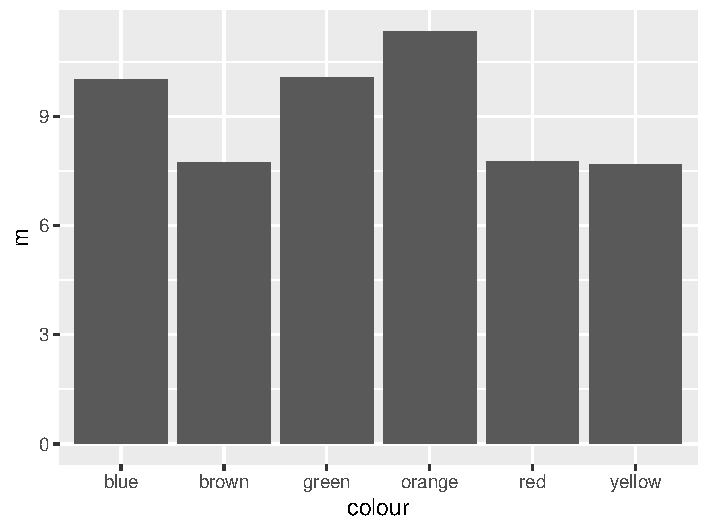
\includegraphics[scale = .75]{graphics/ch3Figs/bar_1.pdf}
\end{figure}

The argument \R{stat = "identity"} is simply telling \textit{ggplot2} to use the values within the \R{skull\_summary} tibble to create the bars.  We needed to specify this because \textit{ggplot2} has the ability to take the raw data directly (e.g., \R{skulls}) and perform its own summary calculations. However, we do not need it to do that in this particular case, hence why we included this argument.

The resulting bar graph displays the mean estimated cranial capacity ($cm^3$) for each period. To enhance its visual appeal, we can adjust the fill colour of the bars to reflect the corresponding time periods more effectively.\footnote{Technically, this is something we should NOT do because, for the sake of comparison, its better to give all the bars the same ``visual weight.'' Keeping all the bars the same colour does precisely that. Moreover, with the \textit{x}-axis labels, there is no reason to add additional elements that could be distracting. That being said, if you are collaborating on a project, your collaborators will probably demand to see colourful bars irrespective this rationale (experience has taught me this). And if they outnumber you, they can probably beat you in a fight - it doesn't matter if you have the moral or logical high ground.} When we do this, we have to be mindful of the fact that the x-axis contains a \textit{discrete} scale, not a \textit{continuous} one like we saw in chapter 2 (for more information on discrete vs. continuous scales see section \ref{sec:pos_scale}).

First we will define our colour palette by creating a vector of hexadecimal colour codes we want to use.

\begin{inR}
egypt_pal <- c(
  "#7E6A58", "#C2B280", "#6A8347", "#A23E2A", "#B04E0F",
  "#2E8B8B", "#264653", "#D4AF37", "#8B8589", "#C9C9C9"
)
\end{inR}

\vspace{1em}

\noindent
We can then us \R{egypt\_pal} to adjust the fill colour of the bars in the plot.

\begin{inR}
ggplot(skull_summary, aes(x = period, y = m)) +
  geom_bar(
    stat = "identity",
    colour = "black",
    aes(fill = period)
  ) +
  scale_fill_manual(values = egypt_pal)
\end{inR}

\vspace{2em}

\begin{figure}[H]
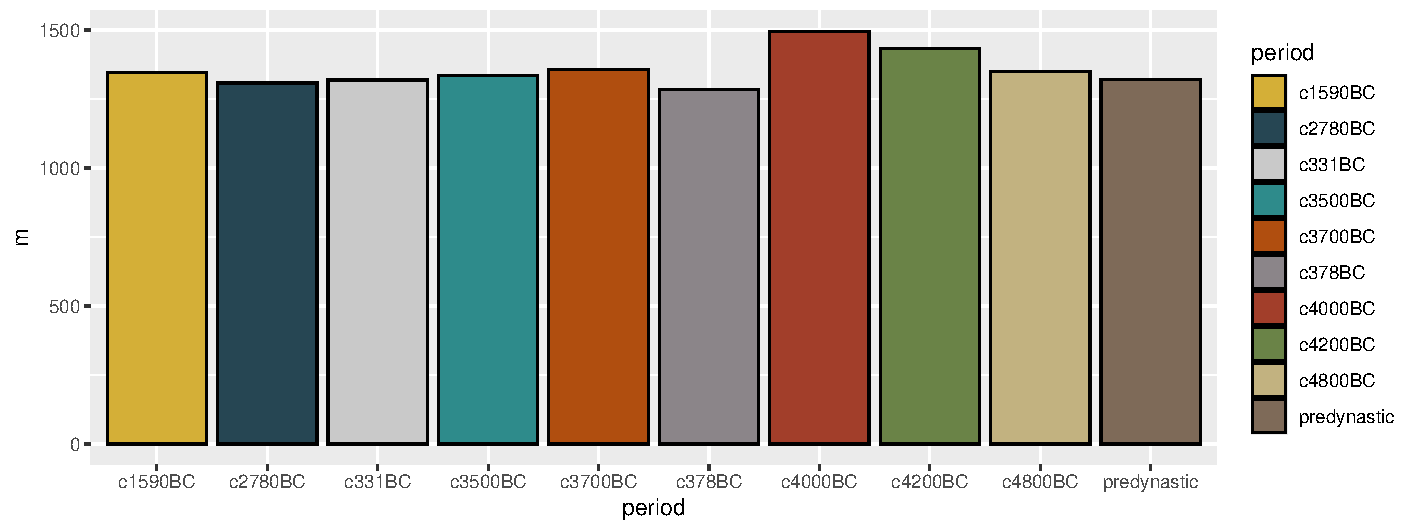
\includegraphics[width = 0.95\textwidth]{graphics/ch3Figs/bar_2.pdf}
\end{figure}

\noindent
\textit{ggplot2} quite sagely adds a legend when you map fill colours to a variable; however, in this particular case the legend is redundant with the information our \textit{x}-axis provides and is thus taking up space unnecessarily. To remove the legend, there are different methods that could be employed. Since we only have the fill aesthetic mapped, it is easy enough to just add \R{guide = "none"} to the \R{scale\_fill\_manual()} function.

\begin{inR}
...
  scale_fill_manual(values = egypt_pal, guide = "none")
\end{inR}

\vspace{2em}

\begin{figure}[H]
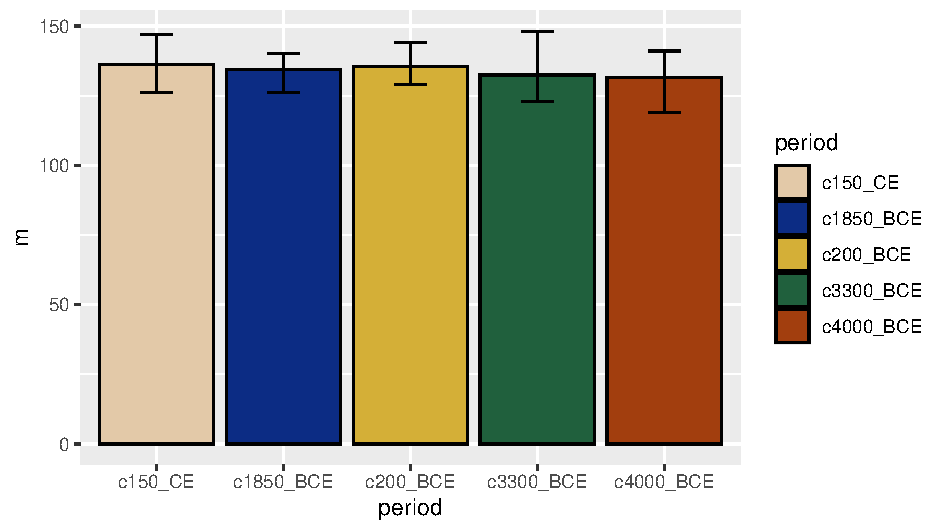
\includegraphics[width = 0.95\textwidth]{graphics/ch3Figs/bar_3.pdf}
\end{figure}

In addition to the mean estimated cranial capacity for each period, \R{skull\_summary} also includes the smallest and largest measured capacities, stored in the \R{\$min} and \R{\$max} columns, respectively. We can incorporate this information into our graph using \glspl{error bar}. Error bars provide a visual representation of the data's \textit{spread}, and the difference between the minimum and maximum values corresponds to a classic measure of spread known as the \textit{range}.\footnote{If this concept isn’t entirely clear yet, don’t worry—spread, as a formal statistical idea, will be explored in more detail in later chapters.} While the range is generally not recommended as a primary measure of spread, it has the advantage of being intuitive and serves our current illustrative purposes well enough.

To create error bars, we can simply use \textit{ggplot2's} \R{geom\_errorbar()} function. We just need to tell it which column corresponds to the bottom of the error bars, using the argument \R{ymin}, and which column corresponds to the top of the error bars, using the argument \R{ymax}.

\begin{inR}
ggplot(skull_summary, aes(x = period, y = m)) +
  geom_bar(
    stat = "identity",
    colour = "black",
    aes(fill = period)
  ) +
  scale_fill_manual(values = egypt_pal, guide = "none") +
  geom_errorbar(aes(ymin = min, ymax = max), width = 0.25)
\end{inR}

\vspace{2em}

\begin{figure}[H]
\includegraphics[width = 0.95\textwidth]{graphics/ch3Figs/bar_4.pdf}
\end{figure}

All that remains is to update the plot’s labelling. Specifically, we should provide clearer titles for the $x$- and $y$-axes and adjust the $x$-axis labels to promote better readability.

To change the current labels ``c1590BC'', ``c2780BC'', ``c331BC'' and so on, we can use the \R{labels} argument inside the \R{scale\_x\_discrete()} function. We just have to give it a character vector containing the new labelling in the current order.

\begin{inR}
ggplot(skull_summary, aes(x = period, y = m)) +
  geom_bar(
    stat = "identity",
    colour = "black",
    aes(fill = period)
  ) +
  scale_fill_manual(values = egypt_pal, guide = "none") +
  geom_errorbar(aes(ymin = min, ymax = max), width = 0.25) +
  scale_x_discrete(
    labels = c(
      "c.1590 BC", "c.2780 BC", "c.331 BC", "c.3500 BC", "c.3700 BC",
      "c.378 BC", "c.4000 BC", "c.4200 BC", "c.4800 BC", "Predynastic"
    )
  ) +
  labs(
    x = "Period",
    y = "Cranial Capacity (cm³)"
  )
\end{inR}

\vspace{2em}

\begin{figure}[H]
\includegraphics[width = 0.95\textwidth]{graphics/ch3Figs/bar_5.pdf}
\end{figure}

Having now read Chapter 2 and this chapter, there is still one important plotting detail that remains unaddressed: how to control the order of categories. At the moment, the time periods appear in a non-chronological order (from left to right), which may not align with our expectations or or intentions. So how do we fix that? This is where the concept of \textit{factors} becomes essential.

\section{Factors}

In statistics, we often refer to a categorical variable as a \gls{factor}.\footnote{Variables are often called factors when they represent a fixed set of categories—such as groupings defined by experimental conditions—or when they are technically continuous but take on only a limited number of distinct values. If this seems unclear for now, don’t worry; we’ll explore variable types in more detail in a later chapter.} Factors consist of different \glspl{level}, which correspond to the unique categories that variable can take.

For example, in our tidy data, the variable \R{\$period} can be considered a factor. Each distinct time period in that column—such as \R{predynastic}, \R{c4800BC}, \R{c4200BC}, \R{c4000BC}, and so on—represents a different level of the factor. That is, the factor named \R{\$period} has multiple levels, one for each unique period label.

To summarize: in tidy data, you can think of a ``factor'' as essentially a categorical variable (or column), and a ``level'' as one of its possible categories. Just beware that this terminology is specific to tidy data structures.

\clearpage

{
\begin{itemize}
  \setlength\itemsep{-1em}
    \item Factor = column
    \item Level = category within a column
\end{itemize}
}

\noindent
If we examine \R{skulls}:

\begin{inR}
skulls
\end{inR}
\begin{outR}
# A tibble: 1,449 × 3
   sex   period      capacity
   <chr> <chr>          <dbl>
 1 Male  predynastic     1370
 2 Male  c4800BC         1410
 3 Male  c4200BC         1320
 4 Male  c4000BC         1445
 5 Male  c3500BC         1395
 6 Male  c2780BC         1425
 7 Male  c1590BC         1440
 8 Male  c378BC          1310
 9 Male  c331BC          1450
10 Male  predynastic     1250
# i 1,439 more rows
# i Use `print(n = ...)` to see more rows
\end{outR}

\noindent
You can see that the output is telling us that the \R{\$period} column is a character vector (notice the \R{<chr>}). In other words, R does not know that \R{predynastic}, \R{c4800BC}, \R{c4200BC}, etc. are categories. It just sees 1,449 individual character values in that particular column. For the purpose of plotting and analyses, it is important that R understands that these are levels of a factor (i.e., it is important that it treats these as categories). We can easily tell R that a particular column is a factor using the function \R{factor()}.\footnote{Technically, when we use this function we are replacing an existing column with a new column that happens to be a class of object called a factor. We are not really ``telling'' R it is a factor, we are ``creating'' a factor - but that's just a nitpicky semantic issue.}

\begin{inR}
skulls$period <- factor(skulls$period)
skulls
\end{inR}
\begin{outR}
# A tibble: 1,449 × 3
   sex   period      capacity
   <chr> <fct>          <dbl>
 1 Male  predynastic     1370
 2 Male  c4800BC         1410
 3 Male  c4200BC         1320
 4 Male  c4000BC         1445
 5 Male  c3500BC         1395
 6 Male  c2780BC         1425
 7 Male  c1590BC         1440
 8 Male  c378BC          1310
 9 Male  c331BC          1450
10 Male  predynastic     1250
# i 1,439 more rows
# i Use `print(n = ...)` to see more rows
\end{outR}


\noindent
Notice that the \R{\$period} column is now labelled as \R{<fct>}, which stands for ``factor.'' Additionally, if we isolate this column, the ten levels of the factor are displayed at the bottom of the output.

\begin{inR}
skulls$period
\end{inR}
\begin{outR}
...
10 Levels: c1590BC c2780BC c331BC c3500BC c3700BC ... predynastic
\end{outR}

\noindent
While this implicit listing is convenient, a better and more deliberate way to view the levels of a factor is to use the \R{levels()} function.

\begin{inR}
levels(skulls$period)
\end{inR}
\begin{outR}
 [1] "c1590BC"     "c2780BC"     "c331BC"      "c3500BC"     "c3700BC"    
 [6] "c378BC"      "c4000BC"     "c4200BC"     "c4800BC"     "predynastic"
\end{outR}

\subsection{Ordering Levels}

Discerning readers may have noticed that the order of the levels shown match the order of the bars in the graph we created. This is not a coincidence. Whenever you use \textit{ggplot2} to plot or \textit{dplyr} to summarize categorical data, these packages quietly convert the relevant columns into factors behind the scenes. By default, R arranges factor levels in alphabetical order, which is why the bars appeared in that particular sequence. However, we can override this default by explicitly specifying the order of the levels when we define the factor using the \R{factor()} function. This allows us to arrange categories in a more meaningful way—such as placing historical time periods in chronological order.

\begin{inR}
skulls$period <- factor(skulls$period,
  levels = c(
    "predynastic", "c4800BC", "c4200BC", "c4000BC", "c3700BC",
    "c3500BC", "c2780BC", "c1590BC", "c378BC", "c331BC"
  )
)
levels(skulls$period)
\end{inR}

\begin{outR}
 [1] "predynastic" "c4800BC"     "c4200BC"     "c4000BC"     "c3700BC"    
 [6] "c3500BC"     "c2780BC"     "c1590BC"     "c378BC"      "c331BC" 
\end{outR}

It is important to emphasize that reordering the levels of a factor does \textit{not} change the actual order of the values in the data frame. The rows remain exactly as they were. What we are doing instead is instructing R that, for the purposes of plotting or analysis, \R{predynastic} should be treated as coming before \R{c4800BC}, which comes before \R{c4200BC}, and so on. If we now re-run our earlier code to compute summary statistics, you will see that the \R{\$period} column reflects this new ordering and is listed as \R{<fct>}.

\begin{inR}
skull_summary <- skulls |>
  group_by(period) |>
  summarise(
    m = mean(capacity),
    n = length(capacity),
    N = nrow(skulls),
    m_heq = m / 4800,
    med_heq = median(capacity) / 4800,
    min = min(capacity),
    max = max(capacity)
  )

skull_summary
\end{inR}

\begin{outR}
# A tibble: 10 × 8
   period        m     n     N m_heq med_heq   min   max
   <fct>     <dbl> <int> <int> <dbl>   <dbl> <dbl> <dbl>
 1 predynas… 1320.   318  1449 0.275   0.273  1050  1710
 2 c4800BC   1349.   124  1449 0.281   0.283  1110  1640
 3 c4200BC   1434.    16  1449 0.299   0.306  1110  1740
 4 c4000BC   1495.    50  1449 0.311   0.311  1235  1775
 5 c3700BC   1356.     7  1449 0.283   0.284  1245  1450
 6 c3500BC   1337.   315  1449 0.278   0.277   965  1760
 7 c2780BC   1308.   152  1449 0.273   0.270  1030  1660
 8 c1590BC   1347.   203  1449 0.281   0.280  1080  1665
 9 c378BC    1286.    32  1449 0.268   0.266  1095  1550
10 c331BC    1319.   232  1449 0.275   0.275  1000  1570
\end{outR}

\noindent
Moreover, when we now plot the data, the bars will also have shifted their position accordingly.

\begin{inR}
ggplot(skull_summary, aes(x = period, y = m)) +
  geom_bar(stat = "identity")
\end{inR}

\vspace{2em}

\begin{figure}[H]
\includegraphics[width = 0.95\textwidth]{graphics/ch3Figs/bar_6.pdf}
\end{figure}

\subsection{Naming Levels}

On occasion, it will be useful to rename the levels of a factor. For instance, previously we had used the \R{labels} argument inside \textit{ggplot2}'s \R{scale\_x\_discrete()} function to adjust the \textit{x}-axis labelling. However, an alternative strategy would have been to relabel the factor levels. We can do this using the \R{levels()} function from earlier. And we have the option of renaming the levels of the \R{skulls} or \R{skull\_summary} data frames. We will do the latter so that we do not need to re-run the code that produced \R{skull\_summary}.

\begin{inR}
levels(skull_summary$period) <- c(
  "Predynastic", "c.4800 BC", "c.4200 BC", "c.4000 BC", "c.3700 BC",
  "c.3500 BC", "c.2780 BC", "c.1590 BC", "c.378 BC", "c.331 BC"
)
skull_summary
\end{inR}
\begin{outR}
# A tibble: 10 × 8
   period          m     n     N m_heq med_heq   min   max
   <fct>       <dbl> <int> <int> <dbl>   <dbl> <dbl> <dbl>
 1 Predynastic 1320.   318  1449 0.275   0.273  1050  1710
 2 c.4800 BC   1349.   124  1449 0.281   0.283  1110  1640
 3 c.4200 BC   1434.    16  1449 0.299   0.306  1110  1740
 4 c.4000 BC   1495.    50  1449 0.311   0.311  1235  1775
 5 c.3700 BC   1356.     7  1449 0.283   0.284  1245  1450
 6 c.3500 BC   1337.   315  1449 0.278   0.277   965  1760
 7 c.2780 BC   1308.   152  1449 0.273   0.270  1030  1660
 8 c.1590 BC   1347.   203  1449 0.281   0.280  1080  1665
 9 c.378 BC    1286.    32  1449 0.268   0.266  1095  1550
10 c.331 BC    1319.   232  1449 0.275   0.275  1000  1570
\end{outR}

\clearpage

\noindent
A corresponding change will be seen on the plot's \textit{x}-axis labels as well when that is generated.

\begin{inR}
ggplot(skull_summary, aes(x = period, y = m)) +
  geom_bar(
    stat = "identity",
    colour = "black",
    aes(fill = period)
  ) +
  scale_fill_manual(values = egypt_pal, guide = "none") +
  geom_errorbar(aes(ymin = min, ymax = max), width = 0.25) +
  labs(
    x = "Period",
    y = "Cranial Capacity (cm³)"
  )
\end{inR}

\vspace{2em}

\begin{figure}[H]
\includegraphics[width = 0.95\textwidth]{graphics/ch3Figs/bar_7.pdf}
\end{figure}

A brief word of warning is in order: \textbf{do not} confuse the \R{levels} \textit{argument} used inside the \R{factor()} function with the \R{levels()} \textit{function} itself. While they sound similar, they serve very different purposes.\footnote{To further complicate things (because of course it does), the \R{factor()} function also includes a \R{labels} argument that allows you to rename levels at the time of creation. See the R documentation for details: \R{?factor}}

\begin{itemize}
    \item \R{levels = ...} (argument inside \R{factor()}) is used to \textit{specify the order} of factor levels.
    \item \R{levels()} (function) is used to \textit{rename} existing factor levels.
\end{itemize}

\noindent
It is also worth noting that the \href{https://forcats.tidyverse.org/}{\textit{forcats}} package—automatically loaded with the \textit{tidyverse}—offers a variety of useful functions specifically designed for working with factors.

For beginners, factors can feel particularly troublesome: they are cryptic, temperamental, and always popping up when least expected. But they are also foundational to R's thaumaturgy and cannot be avoided. So rather than resisting, it is best to embrace their evil, arcane \mbox{nature}—only then will you be at peace.

\clearpage

\section{Putting It All Together}

To consolidate everything covered in this chapter, it's helpful to revisit the analysis one final time—but in a more realistic, streamlined, end-to-end format. Doing so not only reinforces how the various components work together in a complete R script, but also provides an opportunity to enhance the graph by incorporating some faceting based on the previously ignored variable \R{\$sex}.\footnote{Facets were covered in Chapter 2, section \ref{sec:facets}.}

\begin{inR}
# Load the tidyverse
library(tidyverse)
\end{inR}

\begin{inR}
# Load the data
skulls <- read_csv("skull_cap_partial_wide.csv") |>
  # Pivot to the tidy format
  pivot_longer(
    cols = predynastic:c331BC,
    names_to = "period",
    values_to = "capacity"
  ) |>
  # Remove NAs
  drop_na(capacity)
\end{inR}

\begin{inR}
# Factor and order "period"
skulls$period <- factor(skulls$period,
  levels = c(
    "predynastic", "c4800BC", "c4200BC", "c4000BC", "c3700BC",
    "c3500BC",     "c2780BC", "c1590BC", "c378BC",  "c331BC"
  )
)
\end{inR}

\begin{inR}
# Rename the factor levels
levels(skulls$period) <- c(
  "Predynastic", "c.4800 BC", "c.4200 BC", "c.4000 BC", "c.3700 BC",
  "c.3500 BC",   "c.2780 BC", "c.1590 BC", "c.378 BC",  "c.331 BC"
)
\end{inR}

\begin{inR}
# Calculate stats for plot, grouping by 'period' and 'sex'
skull_summary <- skulls |>
  group_by(period, sex) |> # Note the addition of a second factor to group_by
  summarise(
    m = mean(capacity),
    min = min(capacity),
    max = max(capacity)
  )

skull_summary # Output shows group-wise means and ranges, separated by sex
\end{inR}

\begin{outR}
# A tibble: 18 × 5
# Groups:   period [10]
   period      sex        m   min   max
   <fct>       <chr>  <dbl> <dbl> <dbl>
 1 Predynastic Female 1262.  1050  1570
 2 Predynastic Male   1391.  1130  1710
 3 c.4800 BC   Female 1280.  1110  1515
 4 c.4800 BC   Male   1430.  1195  1640
 5 c.4200 BC   Female 1271   1110  1530
 6 c.4200 BC   Male   1509.  1320  1740
 7 c.4000 BC   Male   1495.  1235  1775
 8 c.3700 BC   Female 1356.  1245  1450
 9 c.3500 BC   Female 1255.   965  1490
10 c.3500 BC   Male   1408.  1160  1760
11 c.2780 BC   Female 1252.  1030  1520
12 c.2780 BC   Male   1384.  1160  1660
13 c.1590 BC   Female 1288.  1080  1515
14 c.1590 BC   Male   1421.  1210  1665
15 c.378 BC    Female 1227.  1095  1400
16 c.378 BC    Male   1345.  1190  1550
17 c.331 BC    Female 1245   1000  1455
18 c.331 BC    Male   1383.  1150  1570
\end{outR}

\begin{inR}
# Store desired colours
egypt_pal <- c(
  "#7E6A58", "#C2B280", "#6A8347", "#A23E2A", "#B04E0F",
  "#2E8B8B", "#264653", "#D4AF37", "#8B8589", "#C9C9C9"
)
\end{inR}

\begin{inR}
# Plot data
ggplot(skull_summary, aes(x = period, y = m)) +
  geom_bar(
    stat = "identity",
    colour = "black",
    aes(fill = period)
  ) +
  geom_errorbar(aes(ymin = min, ymax = max), width = 0.25) +
  scale_fill_manual(values = egypt_pal, guide = "none") +
  labs(
    x = "Period",
    y = "Cranial Capacity (cm³)"
  ) +
  facet_wrap(~ sex, ncol = 1) # Note the use of facet_wrap
\end{inR}

\vspace{2em}

\begin{figure}[H]
\includegraphics[width = 0.95\textwidth]{graphics/ch3Figs/bar_8.pdf}
\end{figure}

Finally, it is worth demonstrating just how easily—and dramatically—we can adjust \textit{ggplot2} to suit different analytical goals. As it currently stands, the plot is structured to compare cranial capacity across time periods within each sex. However, with just two minor changes (see line 2 and 14), we can reorient the layout to instead compare the sexes within each time period. Specifically, we place \R{\$sex} on the $x$-axis and facet according to \R{\$period}.

%\footnote{While the data shows that males tend to have slightly larger crania on average, it's worth noting that the sperm whale (\textit{Physeter macrocephalus}) possesses a brain over five times the size of a human’s—and yet it spends much of its time ramming giant squid in total darkness and clicking at 230 decibels. Don't over-interpret this finding. Male skulls may be bigger on average—but before anyone gets too proud, remember: it's what you do with your brain that counts.}

\begin{inR}
# Plot data
ggplot(skull_summary, aes(x = sex, y = m)) +
  geom_bar(
    stat = "identity",
    colour = "black",
    aes(fill = period)
  ) +
  geom_errorbar(aes(ymin = min, ymax = max), width = 0.25) +
  scale_fill_manual(values = egypt_pal, guide = "none") +
  labs(
    x = "Sex",
    y = "Cranial Capacity (cm³)"
  ) +
  facet_wrap(~ period, ncol = 5)
\end{inR}

\vspace{2em}

\begin{figure}[H]
\includegraphics[width = 0.95\textwidth]{graphics/ch3Figs/bar_9.pdf}
\end{figure}

\part{Descriptive Statistics - Seeing Without Asking}

\IMFellEnglish

This part opens the gate to those ancient tools which allow us to extract form from the formless. We do not yet ask questions of the gods; we simply take stock of the offering they have laid before us.

%\chapter{The Basics of Loading and Manipulating Data}
\chapter{Taxonomies of the Profane – Variables, Scales, and Their Unholy Properties}

\IMFellEnglish
\lettrine[lines=5, realheight]{T}{here} is a kind of grim devilry in the act of classification. The moment you categorize a thing—whether it be a small volume of blood, the reaction time of a startle, or the flickering presence of a belief—you strip it from the chaos of the unknown and chain it down, trembling, to a scale. Statisticians call them variables, but do not be fooled: these are not gentle creatures. They are twisted reflections of reality that must be bound in measurement and tortured into order. Nominal. Ordinal. Interval. Ratio. These are the sigils we etch into our grimoires of data, each one whispering what kind of rituals—summations, correlations, regressions—we may dare perform. But beware: misuse the wrong scale, or confuse the nature of your variable, and the results may turn on you, distorted and cursed. This chapter delves into the infernal art of measurement, uncovering the hidden laws that govern how data can be named, ranked, counted, or quantified. Prepare yourself—for to wield statistics is to practice a kind of taxonomy, yes  ... but one written in the ink of madness, precision, and cruelty.

\normalfont

\section{A Practical Problem}

Consider the complete craniometric dataset provided by  \textcite{Thomson1905}, available in the file \R{Thomson\_Randall-MacIver\_1905.csv},\footnote{The data file can be obtained at this book's GitHub repository: \url{https://github.com/statistical-grimoire/book/blob/main/data/Egyptian-skulls}} a ``small'' excerpt of which is displayed in Table \ref{tab:skulls_full}. The file contains a wide range of craniometric measurements along with other useful, and sometimes missing, contextual information, such as the estimated date range for each skull, the ruling dynasty at the time, and the archaeological site of origin. 

%\begin{landscape}
\begin{table}[p]
\centering
\resizebox{\textwidth}{!}{
\begin{tabular}{rrrlllllrrrrrrrrrrrrrlr}
\toprule
table & start\_date & end\_date & start\_era & end\_era & dynasty & location & sex & gol & ool & bbh & mb & biaurb & bizygb & bnl & bal & nah & nh & nw & fai & ga & po & cc\\
\midrule
\cellcolor{gray!10}{1} & \cellcolor{gray!10}{} & \cellcolor{gray!10}{} & \cellcolor{gray!10}{BC} & \cellcolor{gray!10}{BC} & \cellcolor{gray!10}{Early Predynastic} & \cellcolor{gray!10}{Abydos} & \cellcolor{gray!10}{Male} & \cellcolor{gray!10}{178.0} & \cellcolor{gray!10}{177} & \cellcolor{gray!10}{138.0} & \cellcolor{gray!10}{131} & \cellcolor{gray!10}{113} & \cellcolor{gray!10}{120.0} & \cellcolor{gray!10}{98} & \cellcolor{gray!10}{89} & \cellcolor{gray!10}{68.0} & \cellcolor{gray!10}{49} & \cellcolor{gray!10}{23.0} & \cellcolor{gray!10}{91.0} & \cellcolor{gray!10}{76.0} & \cellcolor{gray!10}{A} & \cellcolor{gray!10}{1370}\\
1 &  &  & BC & BC & Early Predynastic & Abydos & Male & 179.0 & 179 & 131.0 & 125 & 111 & 121.0 & 97 & 92 & 67.0 & 48 & 23.0 & 95.0 & 73.0 & B & 1250\\
\cellcolor{gray!10}{1} & \cellcolor{gray!10}{} & \cellcolor{gray!10}{} & \cellcolor{gray!10}{BC} & \cellcolor{gray!10}{BC} & \cellcolor{gray!10}{Early Predynastic} & \cellcolor{gray!10}{Abydos} & \cellcolor{gray!10}{Male} & \cellcolor{gray!10}{185.0} & \cellcolor{gray!10}{185} & \cellcolor{gray!10}{134.0} & \cellcolor{gray!10}{136} & \cellcolor{gray!10}{112} & \cellcolor{gray!10}{116.0} & \cellcolor{gray!10}{} & \cellcolor{gray!10}{} & \cellcolor{gray!10}{68.0} & \cellcolor{gray!10}{47} & \cellcolor{gray!10}{24.0} & \cellcolor{gray!10}{} & \cellcolor{gray!10}{} & \cellcolor{gray!10}{} & \cellcolor{gray!10}{1430}\\
1 &  &  & BC & BC & Early Predynastic & Abydos & Male & 183.0 & 180 & 132.0 & 131 & 112 & 122.0 & 103 & 99 & 64.0 & 50 & 26.0 & 96.0 & 74.5 & C & 1350\\
\cellcolor{gray!10}{1} & \cellcolor{gray!10}{} & \cellcolor{gray!10}{} & \cellcolor{gray!10}{BC} & \cellcolor{gray!10}{BC} & \cellcolor{gray!10}{Early Predynastic} & \cellcolor{gray!10}{Abydos} & \cellcolor{gray!10}{Male} & \cellcolor{gray!10}{169.0} & \cellcolor{gray!10}{169} & \cellcolor{gray!10}{132.0} & \cellcolor{gray!10}{119} & \cellcolor{gray!10}{106} & \cellcolor{gray!10}{119.0} & \cellcolor{gray!10}{100} & \cellcolor{gray!10}{96} & \cellcolor{gray!10}{64.0} & \cellcolor{gray!10}{44} & \cellcolor{gray!10}{25.0} & \cellcolor{gray!10}{96.0} & \cellcolor{gray!10}{74.0} & \cellcolor{gray!10}{B C} & \cellcolor{gray!10}{1130}\\
\addlinespace
1 &  &  & BC & BC & Early Predynastic & Abydos & Male & 202.0 & 202 & 143.0 & 136 & 119 & 130.0 & 107 & 100 & 75.0 & 54 & 24.0 & 93.0 & 73.5 & A & 1670\\
\cellcolor{gray!10}{1} & \cellcolor{gray!10}{} & \cellcolor{gray!10}{} & \cellcolor{gray!10}{BC} & \cellcolor{gray!10}{BC} & \cellcolor{gray!10}{Early Predynastic} & \cellcolor{gray!10}{Abydos} & \cellcolor{gray!10}{Male} & \cellcolor{gray!10}{185.0} & \cellcolor{gray!10}{185} & \cellcolor{gray!10}{} & \cellcolor{gray!10}{114} & \cellcolor{gray!10}{} & \cellcolor{gray!10}{} & \cellcolor{gray!10}{} & \cellcolor{gray!10}{} & \cellcolor{gray!10}{68.0} & \cellcolor{gray!10}{47} & \cellcolor{gray!10}{23.0} & \cellcolor{gray!10}{} & \cellcolor{gray!10}{} & \cellcolor{gray!10}{} & \cellcolor{gray!10}{}\\
1 &  &  & BC & BC & Early Predynastic & Abydos & Male & 175.0 & 175 &  & 128 &  &  &  &  &  &  &  &  &  &  & \\
\cellcolor{gray!10}{1} & \cellcolor{gray!10}{} & \cellcolor{gray!10}{} & \cellcolor{gray!10}{BC} & \cellcolor{gray!10}{BC} & \cellcolor{gray!10}{Early Predynastic} & \cellcolor{gray!10}{Abydos} & \cellcolor{gray!10}{Male} & \cellcolor{gray!10}{190.0} & \cellcolor{gray!10}{190} & \cellcolor{gray!10}{} & \cellcolor{gray!10}{146} & \cellcolor{gray!10}{} & \cellcolor{gray!10}{} & \cellcolor{gray!10}{} & \cellcolor{gray!10}{} & \cellcolor{gray!10}{} & \cellcolor{gray!10}{} & \cellcolor{gray!10}{} & \cellcolor{gray!10}{} & \cellcolor{gray!10}{} & \cellcolor{gray!10}{} & \cellcolor{gray!10}{}\\
1 &  &  & BC & BC & Early Predynastic & Abydos & Male & 188.0 & 188 &  & 127 &  &  &  &  &  &  &  &  &  &  & \\
\addlinespace
\cellcolor{gray!10}{1} & \cellcolor{gray!10}{} & \cellcolor{gray!10}{} & \cellcolor{gray!10}{BC} & \cellcolor{gray!10}{BC} & \cellcolor{gray!10}{Early Predynastic} & \cellcolor{gray!10}{Abydos} & \cellcolor{gray!10}{Male} & \cellcolor{gray!10}{177.0} & \cellcolor{gray!10}{177} & \cellcolor{gray!10}{122.0} & \cellcolor{gray!10}{130} & \cellcolor{gray!10}{} & \cellcolor{gray!10}{} & \cellcolor{gray!10}{} & \cellcolor{gray!10}{} & \cellcolor{gray!10}{} & \cellcolor{gray!10}{} & \cellcolor{gray!10}{} & \cellcolor{gray!10}{} & \cellcolor{gray!10}{} & \cellcolor{gray!10}{} & \cellcolor{gray!10}{1195}\\
1 &  &  & BC & BC & Early Predynastic & Abydos & Male & 192.0 & 189 &  & 136 &  &  &  &  &  &  &  &  &  &  & \\
\cellcolor{gray!10}{1} & \cellcolor{gray!10}{} & \cellcolor{gray!10}{} & \cellcolor{gray!10}{BC} & \cellcolor{gray!10}{BC} & \cellcolor{gray!10}{Early Predynastic} & \cellcolor{gray!10}{Abydos} & \cellcolor{gray!10}{Male} & \cellcolor{gray!10}{187.0} & \cellcolor{gray!10}{187} & \cellcolor{gray!10}{137.0} & \cellcolor{gray!10}{138} & \cellcolor{gray!10}{114} & \cellcolor{gray!10}{123.0} & \cellcolor{gray!10}{96} & \cellcolor{gray!10}{89} & \cellcolor{gray!10}{76.0} & \cellcolor{gray!10}{56} & \cellcolor{gray!10}{25.0} & \cellcolor{gray!10}{93.0} & \cellcolor{gray!10}{70.5} & \cellcolor{gray!10}{A} & \cellcolor{gray!10}{1500}\\
1 &  &  & BC & BC & Early Predynastic & Abydos & Male & 176.0 & 174 & 134.0 & 132 & 100 &  & 98 & 86 & 65.0 &  &  & 88.0 & 79.5 & - A & 1325\\
\cellcolor{gray!10}{1} & \cellcolor{gray!10}{} & \cellcolor{gray!10}{} & \cellcolor{gray!10}{BC} & \cellcolor{gray!10}{BC} & \cellcolor{gray!10}{Early Predynastic} & \cellcolor{gray!10}{Abydos} & \cellcolor{gray!10}{Male} & \cellcolor{gray!10}{192.0} & \cellcolor{gray!10}{192} & \cellcolor{gray!10}{130.0} & \cellcolor{gray!10}{139} & \cellcolor{gray!10}{115} & \cellcolor{gray!10}{125.0} & \cellcolor{gray!10}{103} & \cellcolor{gray!10}{108} & \cellcolor{gray!10}{72.0} & \cellcolor{gray!10}{48} & \cellcolor{gray!10}{28.0} & \cellcolor{gray!10}{105.0} & \cellcolor{gray!10}{66.0} & \cellcolor{gray!10}{E F} & \cellcolor{gray!10}{1480}\\
\addlinespace
1 &  &  & BC & BC & Early Predynastic & Abydos & Male & 187.0 & 187 &  & 132 &  &  &  &  &  &  &  &  &  &  & \\
\cellcolor{gray!10}{1} & \cellcolor{gray!10}{} & \cellcolor{gray!10}{} & \cellcolor{gray!10}{BC} & \cellcolor{gray!10}{BC} & \cellcolor{gray!10}{Early Predynastic} & \cellcolor{gray!10}{Abydos} & \cellcolor{gray!10}{Male} & \cellcolor{gray!10}{187.0} & \cellcolor{gray!10}{185} & \cellcolor{gray!10}{136.0} & \cellcolor{gray!10}{125} & \cellcolor{gray!10}{105} & \cellcolor{gray!10}{119.0} & \cellcolor{gray!10}{101} & \cellcolor{gray!10}{93} & \cellcolor{gray!10}{66.0} & \cellcolor{gray!10}{48} & \cellcolor{gray!10}{25.0} & \cellcolor{gray!10}{92.0} & \cellcolor{gray!10}{76.0} & \cellcolor{gray!10}{A} & \cellcolor{gray!10}{1350}\\
1 &  &  & BC & BC & Early Predynastic & Abydos & Male & 181.0 & 177 & 134.0 & 131 & 112 & 125.0 & 102 & 102 & 76.0 & 51 & 25.0 & 100.0 & 68.0 & C & 1350\\
\cellcolor{gray!10}{1} & \cellcolor{gray!10}{} & \cellcolor{gray!10}{} & \cellcolor{gray!10}{BC} & \cellcolor{gray!10}{BC} & \cellcolor{gray!10}{Early Predynastic} & \cellcolor{gray!10}{Abydos} & \cellcolor{gray!10}{Male} & \cellcolor{gray!10}{194.0} & \cellcolor{gray!10}{191} & \cellcolor{gray!10}{134.0} & \cellcolor{gray!10}{134} & \cellcolor{gray!10}{127} & \cellcolor{gray!10}{} & \cellcolor{gray!10}{109} & \cellcolor{gray!10}{99} & \cellcolor{gray!10}{72.0} & \cellcolor{gray!10}{51} & \cellcolor{gray!10}{26.0} & \cellcolor{gray!10}{91.0} & \cellcolor{gray!10}{77.5} & \cellcolor{gray!10}{A} & \cellcolor{gray!10}{1480}\\
1 &  &  & BC & BC & Early Predynastic & Abydos & Male & 191.0 & 189 &  & 130 &  &  &  &  &  &  &  &  &  &  & \\
\addlinespace
\cellcolor{gray!10}{1} & \cellcolor{gray!10}{} & \cellcolor{gray!10}{} & \cellcolor{gray!10}{BC} & \cellcolor{gray!10}{BC} & \cellcolor{gray!10}{Early Predynastic} & \cellcolor{gray!10}{EL Amrah} & \cellcolor{gray!10}{Male} & \cellcolor{gray!10}{161.0} & \cellcolor{gray!10}{161} & \cellcolor{gray!10}{} & \cellcolor{gray!10}{129} & \cellcolor{gray!10}{} & \cellcolor{gray!10}{} & \cellcolor{gray!10}{} & \cellcolor{gray!10}{} & \cellcolor{gray!10}{} & \cellcolor{gray!10}{} & \cellcolor{gray!10}{} & \cellcolor{gray!10}{} & \cellcolor{gray!10}{} & \cellcolor{gray!10}{} & \cellcolor{gray!10}{}\\
1 &  &  & BC & BC & Early Predynastic & EL Amrah & Male & 181.0 & 180 & 138.0 & 129 &  & 123.0 & 106 & 95 & 65.0 & 50 & 24.0 & 90.0 & 80.0 & A & 1370\\
\cellcolor{gray!10}{1} & \cellcolor{gray!10}{} & \cellcolor{gray!10}{} & \cellcolor{gray!10}{BC} & \cellcolor{gray!10}{BC} & \cellcolor{gray!10}{Early Predynastic} & \cellcolor{gray!10}{EL Amrah} & \cellcolor{gray!10}{Male} & \cellcolor{gray!10}{188.0} & \cellcolor{gray!10}{188} & \cellcolor{gray!10}{138.0} & \cellcolor{gray!10}{135} & \cellcolor{gray!10}{} & \cellcolor{gray!10}{113.0} & \cellcolor{gray!10}{} & \cellcolor{gray!10}{} & \cellcolor{gray!10}{67.0} & \cellcolor{gray!10}{47} & \cellcolor{gray!10}{26.0} & \cellcolor{gray!10}{} & \cellcolor{gray!10}{} & \cellcolor{gray!10}{} & \cellcolor{gray!10}{1490}\\
1 &  &  & BC & BC & Early Predynastic & EL Amrah & Male & 169.0 &  &  & 140 &  &  &  &  &  &  &  &  &  &  & \\
\cellcolor{gray!10}{1} & \cellcolor{gray!10}{} & \cellcolor{gray!10}{} & \cellcolor{gray!10}{BC} & \cellcolor{gray!10}{BC} & \cellcolor{gray!10}{Early Predynastic} & \cellcolor{gray!10}{EL Amrah} & \cellcolor{gray!10}{Male} & \cellcolor{gray!10}{189.0} & \cellcolor{gray!10}{188} & \cellcolor{gray!10}{} & \cellcolor{gray!10}{138} & \cellcolor{gray!10}{} & \cellcolor{gray!10}{} & \cellcolor{gray!10}{} & \cellcolor{gray!10}{} & \cellcolor{gray!10}{} & \cellcolor{gray!10}{} & \cellcolor{gray!10}{} & \cellcolor{gray!10}{} & \cellcolor{gray!10}{} & \cellcolor{gray!10}{} & \cellcolor{gray!10}{}\\
\addlinespace
1 &  &  & BC & BC & Early Predynastic & EL Amrah & Male & 189.0 & 189 &  & 125 &  &  &  &  &  &  &  &  &  &  & \\
\cellcolor{gray!10}{1} & \cellcolor{gray!10}{} & \cellcolor{gray!10}{} & \cellcolor{gray!10}{BC} & \cellcolor{gray!10}{BC} & \cellcolor{gray!10}{Early Predynastic} & \cellcolor{gray!10}{EL Amrah} & \cellcolor{gray!10}{Male} & \cellcolor{gray!10}{182.0} & \cellcolor{gray!10}{184} & \cellcolor{gray!10}{} & \cellcolor{gray!10}{128} & \cellcolor{gray!10}{} & \cellcolor{gray!10}{} & \cellcolor{gray!10}{} & \cellcolor{gray!10}{} & \cellcolor{gray!10}{} & \cellcolor{gray!10}{} & \cellcolor{gray!10}{} & \cellcolor{gray!10}{} & \cellcolor{gray!10}{} & \cellcolor{gray!10}{} & \cellcolor{gray!10}{}\\
1 &  &  & BC & BC & Early Predynastic & EL Amrah & Male & 195.0 & 193 &  &  &  &  &  &  &  &  &  &  &  &  & \\
\cellcolor{gray!10}{1} & \cellcolor{gray!10}{} & \cellcolor{gray!10}{} & \cellcolor{gray!10}{BC} & \cellcolor{gray!10}{BC} & \cellcolor{gray!10}{Early Predynastic} & \cellcolor{gray!10}{EL Amrah} & \cellcolor{gray!10}{Male} & \cellcolor{gray!10}{193.0} & \cellcolor{gray!10}{191} & \cellcolor{gray!10}{140.5} & \cellcolor{gray!10}{131} & \cellcolor{gray!10}{} & \cellcolor{gray!10}{128.0} & \cellcolor{gray!10}{} & \cellcolor{gray!10}{} & \cellcolor{gray!10}{} & \cellcolor{gray!10}{} & \cellcolor{gray!10}{} & \cellcolor{gray!10}{} & \cellcolor{gray!10}{} & \cellcolor{gray!10}{} & \cellcolor{gray!10}{1495}\\
1 &  &  & BC & BC & Early Predynastic & EL Amrah & Male & 190.0 & 188 &  & 125 &  &  &  &  &  &  &  &  &  &  & \\
\addlinespace
\cellcolor{gray!10}{1} & \cellcolor{gray!10}{} & \cellcolor{gray!10}{} & \cellcolor{gray!10}{BC} & \cellcolor{gray!10}{BC} & \cellcolor{gray!10}{Early Predynastic} & \cellcolor{gray!10}{Hou} & \cellcolor{gray!10}{Male} & \cellcolor{gray!10}{177.0} & \cellcolor{gray!10}{176} & \cellcolor{gray!10}{121.0} & \cellcolor{gray!10}{134} & \cellcolor{gray!10}{116} & \cellcolor{gray!10}{125.0} & \cellcolor{gray!10}{96} & \cellcolor{gray!10}{95} & \cellcolor{gray!10}{72.0} & \cellcolor{gray!10}{53} & \cellcolor{gray!10}{25.0} & \cellcolor{gray!10}{99.0} & \cellcolor{gray!10}{68.0} & \cellcolor{gray!10}{B C} & \cellcolor{gray!10}{1220}\\
1 &  &  & BC & BC & Early Predynastic & Hou & Male & 189.0 & 188 & 129.0 & 126 & 111 & 126.0 & 105 & 109 & 68.0 & 51 & 26.0 & 104.0 & 68.0 & F & 1305\\
\cellcolor{gray!10}{1} & \cellcolor{gray!10}{} & \cellcolor{gray!10}{} & \cellcolor{gray!10}{BC} & \cellcolor{gray!10}{BC} & \cellcolor{gray!10}{Early Predynastic} & \cellcolor{gray!10}{Hou} & \cellcolor{gray!10}{Male} & \cellcolor{gray!10}{190.0} & \cellcolor{gray!10}{188} & \cellcolor{gray!10}{142.0} & \cellcolor{gray!10}{133} & \cellcolor{gray!10}{114} & \cellcolor{gray!10}{} & \cellcolor{gray!10}{106} & \cellcolor{gray!10}{107} & \cellcolor{gray!10}{64.0} & \cellcolor{gray!10}{} & \cellcolor{gray!10}{} & \cellcolor{gray!10}{101.0} & \cellcolor{gray!10}{71.0} & \cellcolor{gray!10}{E} & \cellcolor{gray!10}{1525}\\
1 &  &  & BC & BC & Early Predynastic & Hou & Male & 180.0 & 179 & 136.0 & 132 & 121 & 129.0 & 102 & 100 & 66.0 & 50 & 27.0 & 98.0 & 72.0 & C D & 1375\\
\cellcolor{gray!10}{1} & \cellcolor{gray!10}{} & \cellcolor{gray!10}{} & \cellcolor{gray!10}{BC} & \cellcolor{gray!10}{BC} & \cellcolor{gray!10}{Early Predynastic} & \cellcolor{gray!10}{Hou} & \cellcolor{gray!10}{Male} & \cellcolor{gray!10}{181.0} & \cellcolor{gray!10}{179} & \cellcolor{gray!10}{140.0} & \cellcolor{gray!10}{141} & \cellcolor{gray!10}{114} & \cellcolor{gray!10}{125.0} & \cellcolor{gray!10}{102} & \cellcolor{gray!10}{100} & \cellcolor{gray!10}{72.0} & \cellcolor{gray!10}{51} & \cellcolor{gray!10}{27.0} & \cellcolor{gray!10}{98.0} & \cellcolor{gray!10}{70.0} & \cellcolor{gray!10}{C} & \cellcolor{gray!10}{1520}\\
\addlinespace
1 &  &  & BC & BC & Early Predynastic & Hou & Male & 174.0 & 171 & 134.0 & 131 & 116 & 130.0 & 99 & 97 & 69.0 & 54 & 22.0 & 98.0 & 71.0 & C & 1300\\
\cellcolor{gray!10}{1} & \cellcolor{gray!10}{} & \cellcolor{gray!10}{} & \cellcolor{gray!10}{BC} & \cellcolor{gray!10}{BC} & \cellcolor{gray!10}{Early Predynastic} & \cellcolor{gray!10}{Hou} & \cellcolor{gray!10}{Male} & \cellcolor{gray!10}{178.0} & \cellcolor{gray!10}{178} & \cellcolor{gray!10}{137.0} & \cellcolor{gray!10}{135} & \cellcolor{gray!10}{112} & \cellcolor{gray!10}{122.0} & \cellcolor{gray!10}{109} & \cellcolor{gray!10}{103} & \cellcolor{gray!10}{74.0} & \cellcolor{gray!10}{50} & \cellcolor{gray!10}{24.0} & \cellcolor{gray!10}{94.5} & \cellcolor{gray!10}{74.0} & \cellcolor{gray!10}{A B} & \cellcolor{gray!10}{1400}\\
1 &  &  & BC & BC & Early Predynastic & Hou & Male & 176.0 & 173 & 133.0 & 132 & 112 & 126.0 & 98 & 93 & 72.0 & 53 & 26.0 & 95.0 & 71.5 & A B & 1315\\
\cellcolor{gray!10}{1} & \cellcolor{gray!10}{} & \cellcolor{gray!10}{} & \cellcolor{gray!10}{BC} & \cellcolor{gray!10}{BC} & \cellcolor{gray!10}{Early Predynastic} & \cellcolor{gray!10}{Hou} & \cellcolor{gray!10}{Male} & \cellcolor{gray!10}{181.0} & \cellcolor{gray!10}{179} & \cellcolor{gray!10}{136.0} & \cellcolor{gray!10}{139} & \cellcolor{gray!10}{116} & \cellcolor{gray!10}{} & \cellcolor{gray!10}{98} & \cellcolor{gray!10}{96} & \cellcolor{gray!10}{70.0} & \cellcolor{gray!10}{50} & \cellcolor{gray!10}{27.0} & \cellcolor{gray!10}{98.0} & \cellcolor{gray!10}{70.0} & \cellcolor{gray!10}{} & \cellcolor{gray!10}{1460}\\
1 &  &  & BC & BC & Early Predynastic & Hou & Male & 185.0 & 183 & 131.0 & 132 & 111 & 124.0 & 104 & 101 & 68.0 & 49 & 26.0 & 97.0 & 73.0 & C & 1360\\
\addlinespace
\cellcolor{gray!10}{1} & \cellcolor{gray!10}{} & \cellcolor{gray!10}{} & \cellcolor{gray!10}{BC} & \cellcolor{gray!10}{BC} & \cellcolor{gray!10}{Early Predynastic} & \cellcolor{gray!10}{Hou} & \cellcolor{gray!10}{Male} & \cellcolor{gray!10}{184.0} & \cellcolor{gray!10}{184} & \cellcolor{gray!10}{133.0} & \cellcolor{gray!10}{126} & \cellcolor{gray!10}{114} & \cellcolor{gray!10}{125.0} & \cellcolor{gray!10}{103} & \cellcolor{gray!10}{102} & \cellcolor{gray!10}{66.0} & \cellcolor{gray!10}{51} & \cellcolor{gray!10}{28.0} & \cellcolor{gray!10}{99.0} & \cellcolor{gray!10}{72.0} & \cellcolor{gray!10}{D} & \cellcolor{gray!10}{1310}\\
2 &  &  & BC & BC & Early Predynastic & Hou & Male & 186.0 & 185 & 135.0 & 135 & 116 & 125.0 & 105 & 103 & 66.0 & 47 & 26.0 & 98.0 & 73.0 & D & 1440\\
\cellcolor{gray!10}{2} & \cellcolor{gray!10}{} & \cellcolor{gray!10}{} & \cellcolor{gray!10}{BC} & \cellcolor{gray!10}{BC} & \cellcolor{gray!10}{Early Predynastic} & \cellcolor{gray!10}{Hou} & \cellcolor{gray!10}{Male} & \cellcolor{gray!10}{176.0} & \cellcolor{gray!10}{175} & \cellcolor{gray!10}{124.0} & \cellcolor{gray!10}{134} & \cellcolor{gray!10}{110} & \cellcolor{gray!10}{123.0} & \cellcolor{gray!10}{96} & \cellcolor{gray!10}{93} & \cellcolor{gray!10}{74.0} & \cellcolor{gray!10}{53} & \cellcolor{gray!10}{23.0} & \cellcolor{gray!10}{97.0} & \cellcolor{gray!10}{69.0} & \cellcolor{gray!10}{A B} & \cellcolor{gray!10}{1245}\\
2 &  &  & BC & BC & Early Predynastic & Hou & Male & 187.0 & 186 & 134.0 & 128 &  &  & 110 & 103 & 67.0 & 50 & 27.0 & 94.0 & 77.0 & B C & 1360\\
\cellcolor{gray!10}{2} & \cellcolor{gray!10}{} & \cellcolor{gray!10}{} & \cellcolor{gray!10}{BC} & \cellcolor{gray!10}{BC} & \cellcolor{gray!10}{Early Predynastic} & \cellcolor{gray!10}{Hou} & \cellcolor{gray!10}{Male} & \cellcolor{gray!10}{181.0} & \cellcolor{gray!10}{181} & \cellcolor{gray!10}{130.0} & \cellcolor{gray!10}{130} & \cellcolor{gray!10}{117} & \cellcolor{gray!10}{129.0} & \cellcolor{gray!10}{103} & \cellcolor{gray!10}{104} & \cellcolor{gray!10}{69.0} & \cellcolor{gray!10}{49} & \cellcolor{gray!10}{25.0} & \cellcolor{gray!10}{101.0} & \cellcolor{gray!10}{69.5} & \cellcolor{gray!10}{D E} & \cellcolor{gray!10}{1300}\\
\addlinespace
2 &  &  & BC & BC & Early Predynastic & Hou & Male & 185.0 & 182 & 135.0 & 138 & 121 & 136.0 & 104 & 100 & 78.0 & 55 & 27.0 & 96.0 & 70.0 & A B & 1470\\
\cellcolor{gray!10}{2} & \cellcolor{gray!10}{} & \cellcolor{gray!10}{} & \cellcolor{gray!10}{BC} & \cellcolor{gray!10}{BC} & \cellcolor{gray!10}{Early Predynastic} & \cellcolor{gray!10}{Hou} & \cellcolor{gray!10}{Male} & \cellcolor{gray!10}{184.0} & \cellcolor{gray!10}{184} & \cellcolor{gray!10}{132.0} & \cellcolor{gray!10}{128} & \cellcolor{gray!10}{106} & \cellcolor{gray!10}{117.0} & \cellcolor{gray!10}{97} & \cellcolor{gray!10}{93} & \cellcolor{gray!10}{72.0} & \cellcolor{gray!10}{53} & \cellcolor{gray!10}{25.0} & \cellcolor{gray!10}{96.0} & \cellcolor{gray!10}{70.5} & \cellcolor{gray!10}{A B} & \cellcolor{gray!10}{1320}\\
2 &  &  & BC & BC & Early Predynastic & Hou & Male & 184.0 & 184 & 129.0 & 127 & 116 & 131.0 & 102 & 106 & 63.0 & 48 & 28.0 & 104.0 & 68.5 & F & 1290\\
\cellcolor{gray!10}{2} & \cellcolor{gray!10}{} & \cellcolor{gray!10}{} & \cellcolor{gray!10}{BC} & \cellcolor{gray!10}{BC} & \cellcolor{gray!10}{Early Predynastic} & \cellcolor{gray!10}{Hou} & \cellcolor{gray!10}{Male} & \cellcolor{gray!10}{185.0} & \cellcolor{gray!10}{183} & \cellcolor{gray!10}{136.0} & \cellcolor{gray!10}{131} & \cellcolor{gray!10}{117} & \cellcolor{gray!10}{129.0} & \cellcolor{gray!10}{111} & \cellcolor{gray!10}{114} & \cellcolor{gray!10}{73.0} & \cellcolor{gray!10}{54} & \cellcolor{gray!10}{27.0} & \cellcolor{gray!10}{103.0} & \cellcolor{gray!10}{68.5} & \cellcolor{gray!10}{E F} & \cellcolor{gray!10}{1400}\\
2 &  &  & BC & BC & Early Predynastic & Hou & Male & 180.0 & 179 & 138.0 & 124 & 114 & 120.0 & 101 & 101 & 62.0 & 46 & 25.0 & 100.0 & 71.5 & D E & 1310\\
\addlinespace
\cellcolor{gray!10}{2} & \cellcolor{gray!10}{} & \cellcolor{gray!10}{} & \cellcolor{gray!10}{BC} & \cellcolor{gray!10}{BC} & \cellcolor{gray!10}{Early Predynastic} & \cellcolor{gray!10}{Hou} & \cellcolor{gray!10}{Male} & \cellcolor{gray!10}{181.0} & \cellcolor{gray!10}{180} & \cellcolor{gray!10}{139.0} & \cellcolor{gray!10}{131} & \cellcolor{gray!10}{113} & \cellcolor{gray!10}{121.0} & \cellcolor{gray!10}{98} & \cellcolor{gray!10}{92} & \cellcolor{gray!10}{71.0} & \cellcolor{gray!10}{53} & \cellcolor{gray!10}{24.0} & \cellcolor{gray!10}{94.0} & \cellcolor{gray!10}{73.0} & \cellcolor{gray!10}{A} & \cellcolor{gray!10}{1400}\\
2 &  &  & BC & BC & Early Predynastic & Hou & Male & 183.0 & 182 & 138.0 & 131 & 111 & 126.0 & 102 & 98 & 73.0 & 49 & 24.0 & 96.0 & 71.0 & B & 1410\\
\cellcolor{gray!10}{2} & \cellcolor{gray!10}{} & \cellcolor{gray!10}{} & \cellcolor{gray!10}{BC} & \cellcolor{gray!10}{BC} & \cellcolor{gray!10}{Early Predynastic} & \cellcolor{gray!10}{Hou} & \cellcolor{gray!10}{Male} & \cellcolor{gray!10}{183.0} & \cellcolor{gray!10}{180} & \cellcolor{gray!10}{140.0} & \cellcolor{gray!10}{137} & \cellcolor{gray!10}{127} & \cellcolor{gray!10}{133.0} & \cellcolor{gray!10}{103} & \cellcolor{gray!10}{103} & \cellcolor{gray!10}{74.0} & \cellcolor{gray!10}{52} & \cellcolor{gray!10}{22.0} & \cellcolor{gray!10}{100.0} & \cellcolor{gray!10}{69.0} & \cellcolor{gray!10}{C} & \cellcolor{gray!10}{1495}\\
2 &  &  & BC & BC & Early Predynastic & Hou & Male & 184.0 & 180 & 125.0 & 128 & 112 & 121.0 & 98 & 95 & 64.0 & 44 & 24.0 & 97.0 & 72.5 & C & 1250\\
\cellcolor{gray!10}{2} & \cellcolor{gray!10}{} & \cellcolor{gray!10}{} & \cellcolor{gray!10}{BC} & \cellcolor{gray!10}{BC} & \cellcolor{gray!10}{Late Predynastic} & \cellcolor{gray!10}{El Amrah} & \cellcolor{gray!10}{Male} & \cellcolor{gray!10}{185.0} & \cellcolor{gray!10}{185} & \cellcolor{gray!10}{138.0} & \cellcolor{gray!10}{124} & \cellcolor{gray!10}{115} & \cellcolor{gray!10}{122.0} & \cellcolor{gray!10}{102} & \cellcolor{gray!10}{101} & \cellcolor{gray!10}{67.0} & \cellcolor{gray!10}{48} & \cellcolor{gray!10}{26.0} & \cellcolor{gray!10}{99.0} & \cellcolor{gray!10}{71.0} & \cellcolor{gray!10}{D} & \cellcolor{gray!10}{1350}\\
\addlinespace
2 &  &  & BC & BC & Late Predynastic & El Amrah & Male & 178.0 & 176 &  & 138 &  &  &  &  &  &  &  &  &  &  & \\
\cellcolor{gray!10}{2} & \cellcolor{gray!10}{} & \cellcolor{gray!10}{} & \cellcolor{gray!10}{BC} & \cellcolor{gray!10}{BC} & \cellcolor{gray!10}{Late Predynastic} & \cellcolor{gray!10}{El Amrah} & \cellcolor{gray!10}{Male} & \cellcolor{gray!10}{189.0} & \cellcolor{gray!10}{187} & \cellcolor{gray!10}{134.0} & \cellcolor{gray!10}{133} & \cellcolor{gray!10}{} & \cellcolor{gray!10}{129.0} & \cellcolor{gray!10}{99} & \cellcolor{gray!10}{97} & \cellcolor{gray!10}{65.0} & \cellcolor{gray!10}{48} & \cellcolor{gray!10}{30.0} & \cellcolor{gray!10}{98.0} & \cellcolor{gray!10}{72.0} & \cellcolor{gray!10}{C D} & \cellcolor{gray!10}{1430}\\
2 &  &  & BC & BC & Late Predynastic & El Amrah & Male & 183.0 & 182 &  & 142 &  &  &  &  &  &  &  &  &  &  & \\
\cellcolor{gray!10}{2} & \cellcolor{gray!10}{} & \cellcolor{gray!10}{} & \cellcolor{gray!10}{BC} & \cellcolor{gray!10}{BC} & \cellcolor{gray!10}{Late Predynastic} & \cellcolor{gray!10}{El Amrah} & \cellcolor{gray!10}{Male} & \cellcolor{gray!10}{183.0} & \cellcolor{gray!10}{183} & \cellcolor{gray!10}{} & \cellcolor{gray!10}{141} & \cellcolor{gray!10}{} & \cellcolor{gray!10}{} & \cellcolor{gray!10}{} & \cellcolor{gray!10}{} & \cellcolor{gray!10}{} & \cellcolor{gray!10}{} & \cellcolor{gray!10}{} & \cellcolor{gray!10}{} & \cellcolor{gray!10}{} & \cellcolor{gray!10}{} & \cellcolor{gray!10}{}\\
2 &  &  & BC & BC & Late Predynastic & El Amrah & Male & 194.0 & 194 &  & 134 &  &  &  &  &  &  &  &  &  &  & \\
\addlinespace
\cellcolor{gray!10}{2} & \cellcolor{gray!10}{} & \cellcolor{gray!10}{} & \cellcolor{gray!10}{BC} & \cellcolor{gray!10}{BC} & \cellcolor{gray!10}{Late Predynastic} & \cellcolor{gray!10}{El Amrah} & \cellcolor{gray!10}{Male} & \cellcolor{gray!10}{189.0} & \cellcolor{gray!10}{189} & \cellcolor{gray!10}{134.0} & \cellcolor{gray!10}{138} & \cellcolor{gray!10}{} & \cellcolor{gray!10}{120.0} & \cellcolor{gray!10}{100} & \cellcolor{gray!10}{98} & \cellcolor{gray!10}{67.0} & \cellcolor{gray!10}{45} & \cellcolor{gray!10}{26.0} & \cellcolor{gray!10}{98.0} & \cellcolor{gray!10}{71.0} & \cellcolor{gray!10}{C} & \cellcolor{gray!10}{1490}\\
2 &  &  & BC & BC & Late Predynastic & El Amrah & Male & 190.0 & 190 &  & 132 &  &  &  &  &  &  &  &  &  &  & \\
\cellcolor{gray!10}{2} & \cellcolor{gray!10}{} & \cellcolor{gray!10}{} & \cellcolor{gray!10}{BC} & \cellcolor{gray!10}{BC} & \cellcolor{gray!10}{Late Predynastic} & \cellcolor{gray!10}{El Amrah} & \cellcolor{gray!10}{Male} & \cellcolor{gray!10}{190.0} & \cellcolor{gray!10}{186} & \cellcolor{gray!10}{129.0} & \cellcolor{gray!10}{148} & \cellcolor{gray!10}{130} & \cellcolor{gray!10}{134.0} & \cellcolor{gray!10}{100} & \cellcolor{gray!10}{104} & \cellcolor{gray!10}{69.0} & \cellcolor{gray!10}{51} & \cellcolor{gray!10}{24.0} & \cellcolor{gray!10}{} & \cellcolor{gray!10}{} & \cellcolor{gray!10}{} & \cellcolor{gray!10}{}\\
2 &  &  & BC & BC & Late Predynastic & El Amrah & Male & 172.0 & 171 & 124.0 & 126 & 110 & 117.0 & 98 & 95 & 61.0 & 45 & 27.0 & 97.0 & 74.0 & C D & 1140\\
\cellcolor{gray!10}{2} & \cellcolor{gray!10}{} & \cellcolor{gray!10}{} & \cellcolor{gray!10}{BC} & \cellcolor{gray!10}{BC} & \cellcolor{gray!10}{Late Predynastic} & \cellcolor{gray!10}{El Amrah} & \cellcolor{gray!10}{Male} & \cellcolor{gray!10}{191.0} & \cellcolor{gray!10}{187} & \cellcolor{gray!10}{136.0} & \cellcolor{gray!10}{135} & \cellcolor{gray!10}{115} & \cellcolor{gray!10}{128.0} & \cellcolor{gray!10}{104} & \cellcolor{gray!10}{98} & \cellcolor{gray!10}{71.0} & \cellcolor{gray!10}{52} & \cellcolor{gray!10}{25.0} & \cellcolor{gray!10}{94.0} & \cellcolor{gray!10}{74.0} & \cellcolor{gray!10}{A B} & \cellcolor{gray!10}{1490}\\
\addlinespace
2 &  &  & BC & BC & Late Predynastic & El Amrah & Male & 185.0 & 184 & 145.0 & 132 & 119 & 130.0 & 102 & 100 & 71.0 & 54 & 23.0 & 98.0 & 70.5 & C & 1505\\
\cellcolor{gray!10}{2} & \cellcolor{gray!10}{} & \cellcolor{gray!10}{} & \cellcolor{gray!10}{BC} & \cellcolor{gray!10}{BC} & \cellcolor{gray!10}{Late Predynastic} & \cellcolor{gray!10}{El Amrah} & \cellcolor{gray!10}{Male} & \cellcolor{gray!10}{187.0} & \cellcolor{gray!10}{185} & \cellcolor{gray!10}{} & \cellcolor{gray!10}{134} & \cellcolor{gray!10}{} & \cellcolor{gray!10}{} & \cellcolor{gray!10}{} & \cellcolor{gray!10}{} & \cellcolor{gray!10}{} & \cellcolor{gray!10}{} & \cellcolor{gray!10}{} & \cellcolor{gray!10}{} & \cellcolor{gray!10}{} & \cellcolor{gray!10}{} & \cellcolor{gray!10}{}\\
2 &  &  & BC & BC & Late Predynastic & El Amrah & Male & 187.0 & 189 & 130.0 & 133 &  & 132.0 & 103 & 102 & 71.0 & 48 & 25.0 & 99.0 & 70.0 & C D & 1375\\
\cellcolor{gray!10}{2} & \cellcolor{gray!10}{} & \cellcolor{gray!10}{} & \cellcolor{gray!10}{BC} & \cellcolor{gray!10}{BC} & \cellcolor{gray!10}{Late Predynastic} & \cellcolor{gray!10}{El Amrah} & \cellcolor{gray!10}{Male} & \cellcolor{gray!10}{176.0} & \cellcolor{gray!10}{176} & \cellcolor{gray!10}{134.0} & \cellcolor{gray!10}{131} & \cellcolor{gray!10}{112} & \cellcolor{gray!10}{119.0} & \cellcolor{gray!10}{103} & \cellcolor{gray!10}{96} & \cellcolor{gray!10}{71.0} & \cellcolor{gray!10}{50} & \cellcolor{gray!10}{25.0} & \cellcolor{gray!10}{93.0} & \cellcolor{gray!10}{74.5} & \cellcolor{gray!10}{A B} & \cellcolor{gray!10}{1315}\\
2 &  &  & BC & BC & Late Predynastic & El Amrah & Male & 189.0 & 186 & 137.0 & 133 &  &  & 102 &  &  &  &  &  &  &  & 1465\\
\addlinespace
\cellcolor{gray!10}{2} & \cellcolor{gray!10}{} & \cellcolor{gray!10}{} & \cellcolor{gray!10}{BC} & \cellcolor{gray!10}{BC} & \cellcolor{gray!10}{Late Predynastic} & \cellcolor{gray!10}{El Amrah} & \cellcolor{gray!10}{Male} & \cellcolor{gray!10}{191.0} & \cellcolor{gray!10}{189} & \cellcolor{gray!10}{} & \cellcolor{gray!10}{134} & \cellcolor{gray!10}{} & \cellcolor{gray!10}{} & \cellcolor{gray!10}{} & \cellcolor{gray!10}{} & \cellcolor{gray!10}{} & \cellcolor{gray!10}{} & \cellcolor{gray!10}{} & \cellcolor{gray!10}{} & \cellcolor{gray!10}{} & \cellcolor{gray!10}{} & \cellcolor{gray!10}{}\\
2 &  &  & BC & BC & Late Predynastic & El Amrah & Male & 171.0 & 172 &  & 120 &  &  &  &  &  &  &  &  &  &  & \\
\cellcolor{gray!10}{2} & \cellcolor{gray!10}{} & \cellcolor{gray!10}{} & \cellcolor{gray!10}{BC} & \cellcolor{gray!10}{BC} & \cellcolor{gray!10}{Late Predynastic} & \cellcolor{gray!10}{El Amrah} & \cellcolor{gray!10}{Male} & \cellcolor{gray!10}{173.0} & \cellcolor{gray!10}{173} & \cellcolor{gray!10}{125.0} & \cellcolor{gray!10}{133} & \cellcolor{gray!10}{111} & \cellcolor{gray!10}{119.0} & \cellcolor{gray!10}{95} & \cellcolor{gray!10}{94} & \cellcolor{gray!10}{70.0} & \cellcolor{gray!10}{46} & \cellcolor{gray!10}{24.0} & \cellcolor{gray!10}{99.0} & \cellcolor{gray!10}{69.0} & \cellcolor{gray!10}{C} & \cellcolor{gray!10}{1220}\\
2 &  &  & BC & BC & Late Predynastic & El Amrah & Male & 191.0 & 190 & 120.0 & 144 &  &  & 99 &  &  &  &  &  &  &  & 1400\\
\cellcolor{gray!10}{2} & \cellcolor{gray!10}{} & \cellcolor{gray!10}{} & \cellcolor{gray!10}{BC} & \cellcolor{gray!10}{BC} & \cellcolor{gray!10}{Late Predynastic} & \cellcolor{gray!10}{El Amrah} & \cellcolor{gray!10}{Male} & \cellcolor{gray!10}{196.0} & \cellcolor{gray!10}{195} & \cellcolor{gray!10}{} & \cellcolor{gray!10}{132} & \cellcolor{gray!10}{} & \cellcolor{gray!10}{} & \cellcolor{gray!10}{} & \cellcolor{gray!10}{} & \cellcolor{gray!10}{} & \cellcolor{gray!10}{} & \cellcolor{gray!10}{} & \cellcolor{gray!10}{} & \cellcolor{gray!10}{} & \cellcolor{gray!10}{} & \cellcolor{gray!10}{}\\
\addlinespace
2 &  &  & BC & BC & Late Predynastic & El Amrah & Male & 183.0 & 183 & 136.0 & 136 &  &  &  &  &  &  &  &  &  &  & 1440\\
\cellcolor{gray!10}{2} & \cellcolor{gray!10}{} & \cellcolor{gray!10}{} & \cellcolor{gray!10}{BC} & \cellcolor{gray!10}{BC} & \cellcolor{gray!10}{Late Predynastic} & \cellcolor{gray!10}{El Amrah} & \cellcolor{gray!10}{Male} & \cellcolor{gray!10}{185.0} & \cellcolor{gray!10}{182} & \cellcolor{gray!10}{131.0} & \cellcolor{gray!10}{131} & \cellcolor{gray!10}{} & \cellcolor{gray!10}{127.0} & \cellcolor{gray!10}{104} & \cellcolor{gray!10}{98} & \cellcolor{gray!10}{67.0} & \cellcolor{gray!10}{} & \cellcolor{gray!10}{} & \cellcolor{gray!10}{94.0} & \cellcolor{gray!10}{75.0} & \cellcolor{gray!10}{B} & \cellcolor{gray!10}{1350}\\
2 &  &  & BC & BC & Late Predynastic & El Amrah & Male & 187.0 & 187 & 130.0 & 122 &  & 118.5 & 103 & 91 & 66.5 & 49 & 25.0 & 88.0 & 79.5 & - A & 1260\\
\cellcolor{gray!10}{2} & \cellcolor{gray!10}{} & \cellcolor{gray!10}{} & \cellcolor{gray!10}{BC} & \cellcolor{gray!10}{BC} & \cellcolor{gray!10}{Late Predynastic} & \cellcolor{gray!10}{El Amrah} & \cellcolor{gray!10}{Male} & \cellcolor{gray!10}{194.5} & \cellcolor{gray!10}{192} & \cellcolor{gray!10}{133.0} & \cellcolor{gray!10}{132} & \cellcolor{gray!10}{} & \cellcolor{gray!10}{124.0} & \cellcolor{gray!10}{104} & \cellcolor{gray!10}{104} & \cellcolor{gray!10}{74.0} & \cellcolor{gray!10}{48} & \cellcolor{gray!10}{23.5} & \cellcolor{gray!10}{100.0} & \cellcolor{gray!10}{69.0} & \cellcolor{gray!10}{C} & \cellcolor{gray!10}{1450}\\
2 &  &  & BC & BC & Late Predynastic & El Amrah & Male & 193.0 & 193 & 128.0 & 131 &  &  &  &  &  &  &  &  &  &  & 1380\\
\addlinespace
\cellcolor{gray!10}{2} & \cellcolor{gray!10}{} & \cellcolor{gray!10}{} & \cellcolor{gray!10}{BC} & \cellcolor{gray!10}{BC} & \cellcolor{gray!10}{Late Predynastic} & \cellcolor{gray!10}{El Amrah} & \cellcolor{gray!10}{Male} & \cellcolor{gray!10}{196.0} & \cellcolor{gray!10}{194} & \cellcolor{gray!10}{132.0} & \cellcolor{gray!10}{136} & \cellcolor{gray!10}{} & \cellcolor{gray!10}{126.0} & \cellcolor{gray!10}{} & \cellcolor{gray!10}{} & \cellcolor{gray!10}{} & \cellcolor{gray!10}{} & \cellcolor{gray!10}{} & \cellcolor{gray!10}{} & \cellcolor{gray!10}{} & \cellcolor{gray!10}{} & \cellcolor{gray!10}{1500}\\
2 &  &  & BC & BC & Late Predynastic & El Amrah & Male & 188.0 & 187 & 134.0 & 129 &  &  &  &  &  &  &  &  &  &  & 1380\\
\cellcolor{gray!10}{2} & \cellcolor{gray!10}{} & \cellcolor{gray!10}{} & \cellcolor{gray!10}{BC} & \cellcolor{gray!10}{BC} & \cellcolor{gray!10}{Late Predynastic} & \cellcolor{gray!10}{Hou} & \cellcolor{gray!10}{Male} & \cellcolor{gray!10}{179.0} & \cellcolor{gray!10}{178} & \cellcolor{gray!10}{} & \cellcolor{gray!10}{132} & \cellcolor{gray!10}{111} & \cellcolor{gray!10}{119.0} & \cellcolor{gray!10}{101} & \cellcolor{gray!10}{96} & \cellcolor{gray!10}{66.0} & \cellcolor{gray!10}{50} & \cellcolor{gray!10}{23.0} & \cellcolor{gray!10}{95.0} & \cellcolor{gray!10}{74.0} & \cellcolor{gray!10}{B} & \cellcolor{gray!10}{}\\
2 &  &  & BC & BC & Late Predynastic & Hou & Male & 186.0 & 184 & 136.0 & 133 & 116 & 127.0 & 107 & 103 & 72.0 & 53 & 27.0 & 96.0 & 72.5 & B C & 1430\\
\cellcolor{gray!10}{2} & \cellcolor{gray!10}{} & \cellcolor{gray!10}{} & \cellcolor{gray!10}{BC} & \cellcolor{gray!10}{BC} & \cellcolor{gray!10}{Late Predynastic} & \cellcolor{gray!10}{Hou} & \cellcolor{gray!10}{Male} & \cellcolor{gray!10}{185.0} & \cellcolor{gray!10}{183} & \cellcolor{gray!10}{139.0} & \cellcolor{gray!10}{131} & \cellcolor{gray!10}{118} & \cellcolor{gray!10}{127.0} & \cellcolor{gray!10}{105} & \cellcolor{gray!10}{98} & \cellcolor{gray!10}{70.0} & \cellcolor{gray!10}{51} & \cellcolor{gray!10}{26.0} & \cellcolor{gray!10}{93.0} & \cellcolor{gray!10}{75.0} & \cellcolor{gray!10}{A B} & \cellcolor{gray!10}{1430}\\
\addlinespace
2 &  &  & BC & BC & Late Predynastic & Hou & Male & 187.0 & 185 & 136.0 & 131 & 114 & 124.0 & 102 & 99 & 77.0 & 56 & 25.0 & 97.0 & 69.0 & A B & 1420\\
\cellcolor{gray!10}{2} & \cellcolor{gray!10}{} & \cellcolor{gray!10}{} & \cellcolor{gray!10}{BC} & \cellcolor{gray!10}{BC} & \cellcolor{gray!10}{Late Predynastic} & \cellcolor{gray!10}{Hou} & \cellcolor{gray!10}{Male} & \cellcolor{gray!10}{194.0} & \cellcolor{gray!10}{194} & \cellcolor{gray!10}{134.0} & \cellcolor{gray!10}{138} & \cellcolor{gray!10}{109} & \cellcolor{gray!10}{116.0} & \cellcolor{gray!10}{100} & \cellcolor{gray!10}{98} & \cellcolor{gray!10}{68.0} & \cellcolor{gray!10}{49} & \cellcolor{gray!10}{24.0} & \cellcolor{gray!10}{98.0} & \cellcolor{gray!10}{71.0} & \cellcolor{gray!10}{C} & \cellcolor{gray!10}{1525}\\
2 &  &  & BC & BC & Late Predynastic & Hou & Male & 190.0 & 189 & 136.0 & 130 & 116 & 127.0 & 107 & 104 & 75.0 & 53 & 25.0 & 97.0 & 71.0 & B C & 1430\\
\cellcolor{gray!10}{2} & \cellcolor{gray!10}{} & \cellcolor{gray!10}{} & \cellcolor{gray!10}{BC} & \cellcolor{gray!10}{BC} & \cellcolor{gray!10}{Late Predynastic} & \cellcolor{gray!10}{Hou} & \cellcolor{gray!10}{Male} & \cellcolor{gray!10}{182.0} & \cellcolor{gray!10}{180} & \cellcolor{gray!10}{128.0} & \cellcolor{gray!10}{131} & \cellcolor{gray!10}{111} & \cellcolor{gray!10}{126.0} & \cellcolor{gray!10}{99} & \cellcolor{gray!10}{98} & \cellcolor{gray!10}{63.0} & \cellcolor{gray!10}{45} & \cellcolor{gray!10}{25.0} & \cellcolor{gray!10}{99.0} & \cellcolor{gray!10}{71.0} & \cellcolor{gray!10}{D} & \cellcolor{gray!10}{1300}\\
\bottomrule
\end{tabular}}
\caption{An excerpt showing the first two, of 32, data tables presented in the appendix of \textcite{Thomson1905}.}
\label{tab:skulls_full}
\end{table}
%\end{landscape}


All totalled, there are 23 separate columns of information each with close to 1000 or more values to conduct an analyses with. This raises a couple of important questions:

\begin{enumerate}
    \item What exactly do we mean by ``analyses'' in this context?
    \item Given the sheer number of distinct values, how can we discuss this data in a practical and meaningful way?
\end{enumerate}

Listing the complete set of values each time we want to reference the data would be wildly impractical. And even if we were absurdly committed to doing so, it is safe to say that our meagre primate brains simply are not equipped to juggle that much information at once. What we are after then are clear, compact, and accurate descriptions of the data that still capture its essential features. Put another way, we need to distil the data's chaos into something intelligible. That is the essence of ``conducting'' an analysis and, while this may seem a hopeless task given the sheer volume of data, there is often a surprisingly large amount of order buried within this seeming chaos.

\section{Descriptive and Inferential Analyses}

The analysis of data is typically driven by two main objectives. The first is descriptive: to summarize the data in ways that are intuitive and meaningful. Perhaps unsurprisingly, this is commonly referred to as a \gls{descriptive analysis}. The second objective is inferential: to use those summaries to make conclusions that reach beyond the data at hand. These conclusions are generally assumed to have some form of practical relevance\footnote{While practical relevance should be a requirement for any inferential analysis, many such analyses are performed more out of tradition than genuine purpose. This isn't cynicism—just the voice of experience, tinged with a bit of jadedness.}—for example, by helping to answer a key research question. This process is known as \gls{inferential analysis}, and it always builds upon descriptive analysis as a necessary foundation.

In many respects a \textit{descriptive analysis} should be a purely empirical endeavour. To the best of the analyst’s ability, it seeks to answer a simple question: what can be said with certainty about this data? This often involves computing summary statistics that characterize the dataset as a whole. For example, calculating familiar measures such as the mode, median, and mean, or visualizing the distribution using graphs like histograms, are all methods that tell us something about which values are most commonly observed in the data set and how the values as a whole are distributed.

\textit{Inferential analysis} goes a step further by introducing reasonable assumptions that allow us (the analyst) to make predictions or generalizations that extend beyond the data at hand. In most cases, we are not interested in the dataset for its own sake—we care about what it represents. That is, we want to know what can it tell us about a broader population, what trends might it reveal about an underlying system, what future outcomes might it help us predict? Statistical methods that allow us to extrapolate in this respect are inferential in nature.

\section{Data}

The word data has appeared frequently throughout this book, often without much reflection as to what it actually means. Given that data is the central subject of both \textit{descriptive} and \textit{inferential} analysis, it is perhaps worth taking a moment to clarify. At its core, \gls{data} refers to a collection of observations about \textit{something}. The singular form, \gls{datum}, refers to just one of those observations. The ``something'' in question is usually the phenomenon the researcher is investigating—this could be the number of cells in a slice of brain tissue, the rate of deaths per capita, how quickly participants learn a behavioural response; or any number of other things that can be measured or classified in some way. 

Before going further, it’s worth drawing a distinction between what we will refer to as \textit{statistical data}—the kind typically used in research and analysis (e.g., see Table \ref{tab:msleep} and Table \ref{tab:skulls_full})—and the kind of data used to train machine learning models (e.g., pictures of cats, playlists of Eurodance hits, or whatever else the algorithm gods demand). In the latter case, what is being fed to the model is perhaps more akin to collections of stimuli than it is data in the traditional statistical sense of the term. That said, in machine learning contexts, the terms \textit{data} and \textit{stimuli} are often used interchangeably. When this book refers to ``data'', you can assume it means \textit{statistical data}.\footnote{Yes, I’m aware I haven’t defined ``statistic'' yet. But some knowledge comes at a price—and you haven’t bled nearly enough.}

\section{A Taxonomy of Data}

\subsection{Variables}

Examining Table \ref{tab:skulls_full}, we can see that each row corresponds to a single skull examined by \textcite{Thomson1905}. Each column captures a different type of information recorded for that skull. Some columns contain categorical details—such as the ruling dynasty at the time of burial, the archaeological site where the skull was found, or the presumed sex of the individual—while others include numeric measurements, like the glabello-occipital length (gol), ophryo-occipital length (ool), and basi-bregmatic height (bbh), just to name a few.

Each column in a dataset represents what we call a \gls{variable}—a characteristic or property that can differ (i.e., \textit{vary}) across the observations. It is worth noting that this use of the term ``variable'' is slightly different from how it is used in something like algebra, which is probably the most familiar context in which the term appears. In algebra, a variable is a symbol that stands for an unknown value or set of values (hence the classic phrase ``solve for $x$'', with $x$ being the variable). Still, the two meanings have an underlying connection because, in both cases, we are referring to something—be it a symbol, label, or phrase—that can represent different values. For example, in Table \ref{tab:skulls_full} \textit{sex} is a variable that (from \citeauthor{Thomson1905}'s perspective) has two possible values: ``male'' and ``female.''  Cranial capacity (\textit{cc}) is also a variable, but it is a variable which can take on a theoretically infinite amount of possibilities that extend anywhere from 0 to infinity in the positive direction.\footnote{This is not to suggest that Godzilla-sized skulls are in any way feasible. An asymptote lurks somewhere along the continuum — and long before we reach kaiju level proportions, the laws of physics (and the poor creature’s neck) would surely intervene.}

\subsection{Scales of Measurement}

The way you approach a descriptive or inferential analysis depends critically on the nature of your variables. For example, it makes little sense to try to compute the mean of categorical traits like eye colour, biological sex, or whether a plant specimen is alive or dead. Calculating a mean assumes the data possess certain numerical properties—specifically, that the values lie on a scale where arithmetic operations like addition and division are valid. When those conditions are not met, the result is not just meaningless—it is misleading.

Since the late 1940s, most areas of science have traditionally classified data into four types, known as \textit{scales of measurement}. This framework arose in response to a philosophical dilemma that emerged as the field of Psychology in particular sought to establish itself as a valid scientific discipline. Specifically, the problem revolved around a deceptively simple question: \textit{Is it possible to measure human sensation?} \parencite[p. 677]{Stevens1946}.

To see why this question matters, consider a basic example. Suppose you ask participants in a study to rate their happiness on a 11-point scale, where 0 represents the absence of any happiness and 10 represents the happiest they could
conceivably be. For simplicity, imagine you only have two participants—one selects a 3, the other a 5. A common research practice is to compute the mean average, which in this case would be 4 (see equation \ref{eq:sens_1}). 

\begin{equation}
\frac{3 + 5}{2} = \frac{8}{2} = 4
\label{eq:sens_1}
\end{equation}

\noindent
This seems straightforward enough. The average happiness level across these two people is 4. However, there is a potential problem lurking here: the ``psychological distance'' between the numbers on the scale may not be consistent across individuals. What one person considers a 5, another might interpret as a 4, or as a 6, or as a 7, or as a 8.4, or 2.66, or some other value. That becomes an issue when we calculate a mean because the process of adding the values in the numerator assumes these values have a meaning independent of the person. For instance, if instead the participants had reported 2 and 6 we would similarly arrive at 8 in the numerator (see equation \ref{eq:sens_2}).

\begin{equation}
\frac{2 + 6}{2} = \frac{8}{2} = 4
\label{eq:sens_2}
\end{equation}

\noindent
However, we have no compelling reason to assume that a mathematical equality such as $(3 + 5) = (2 + 6)$ should hold in this context (see \ref{eq:sens_3}), because these numbers reflect \textit{subjective} judgments—not objective quantities grounded in a standardized unit of measurement. Is it mathematically true that both $(3 + 5) = 8$ and $(2 + 6) = 8$? Yes, arithmetically. But in the realm of subjective ratings, such an equality only holds if participants are interpreting the scale in a comparable way. While that is possible, it is far from guaranteed, given the vast differences in individual physiology, psychological states, and lived experience.

\begin{equation}
(3 + 5) \stackrel{?}{=} (2 + 6) \stackrel{?}{=} 8
\label{eq:sens_3}
\end{equation}

\noindent
And the problems do not end there. More fundamentally, there is no objective means of verifying the accuracy—or even the honesty—of any subjective report. We are left to trust that participants are both willing and able to faithfully describe their internal states. This issue, often referred to as the \textit{problem of introspection}, has haunted Psychology since its inception, tracing back to Wilhelm Wundt’s 19th-century laboratory, where the first systematic efforts to understand ``minds'' began.\footnote{One could argue that this problem traces back even earlier, to the foundational work of Ernst Heinrich Weber and Gustav Fechner in psychophysics—research that Wundt deeply admired and which heavily influenced his own.}

None of this is to suggest that subjective assessments should be dismissed outright as pseudoscience. As \textcite{Labovitz1967} contends, there may be some value—however impure—in treating such ratings as more numerical than they truly are. Despite their crude, unstable, and potentially erroneous nature, these measures may still contain just enough precision to tease some signal from the noise. By analogy, the literal sound an engine makes is not what powers a vehicle, but a skilled mechanic can often diagnose a problem from the sound alone. Subjective assessments may be similar in this respect. Introspection is, without doubt, a murky cauldron—but an obsession with methodological purity risks sacrificing potentially useful data on the altar of perfectionism. We ought not discard what might yield insight simply because it falls short of an ideal.

Given what has been said so far, it is hopefully understandable that while not all data conforms to our ideals surrounding numbers and measurement there may still be a certain utility in ascribing numbers to things that are not necessarily quantifiable in the traditional sense. It is often useful to break observations up into sensibile categories and perhaps even order those categories. Along these lines data is usually considered to be either qualitative or quantitive.

Quantiative data is that 







of assigning numbers to magnitudes.


The history of measurement is a long one, dating back to the times of Euclid, and could easily encompass its own textbook.

assigning numbers to magnitudes


%https://plato.stanford.edu/entries/measurement-science/

% Add examples of descriptive and inferential analyses.

% Samples and populations

% Add glossary entries for variables and descriptive and inferential analyses.

% Define qunatitative and qualitative.

%Include section on Random variables?

% \section{Central Tendency and Spread}

% \subsection{Types of Numeric Data}


%https://www.britannica.com/science/sone


% %\chapter{The Basics of Loading and Manipulating Data}
\chapter{Taxonomies of the Profane – Variables, Scales, and Their Unholy Properties}

\IMFellEnglish
\lettrine[lines=5, realheight]{T}{here} is a kind of grim devilry in the act of classification. The moment you categorize a thing—whether it be a small volume of blood, the reaction time of a startle, or the flickering presence of a belief—you strip it from the chaos of the unknown and chain it down, trembling, to a scale. Statisticians call them variables, but do not be fooled: these are not gentle creatures. They are twisted reflections of reality that must be bound in measurement and tortured into order. Nominal. Ordinal. Interval. Ratio. These are the sigils we etch into our grimoires of data, each one whispering what kind of rituals—summations, correlations, regressions—we may dare perform. But beware: misuse the wrong scale, or confuse the nature of your variable, and the results may turn on you, distorted and cursed. This chapter delves into the infernal art of measurement, uncovering the hidden laws that govern how data can be named, ranked, counted, or quantified. Prepare yourself—for to wield statistics is to practice a kind of taxonomy, yes  ... but one written in the ink of madness, precision, and cruelty.

\normalfont

\section{A Practical Problem}

Consider the complete craniometric dataset provided by  \textcite{Thomson1905}, available in the file \R{Thomson\_Randall-MacIver\_1905.csv},\footnote{The data file can be obtained at this book's GitHub repository: \url{https://github.com/statistical-grimoire/book/blob/main/data/Egyptian-skulls}} a ``small'' excerpt of which is displayed in Table \ref{tab:skulls_full}. The file contains a wide range of craniometric measurements along with other useful, and sometimes missing, contextual information, such as the estimated date range for each skull, the ruling dynasty at the time, and the archaeological site of origin. 

%\begin{landscape}
\begin{table}[p]
\centering
\resizebox{\textwidth}{!}{
\begin{tabular}{rrrlllllrrrrrrrrrrrrrlr}
\toprule
table & start\_date & end\_date & start\_era & end\_era & dynasty & location & sex & gol & ool & bbh & mb & biaurb & bizygb & bnl & bal & nah & nh & nw & fai & ga & po & cc\\
\midrule
\cellcolor{gray!10}{1} & \cellcolor{gray!10}{} & \cellcolor{gray!10}{} & \cellcolor{gray!10}{BC} & \cellcolor{gray!10}{BC} & \cellcolor{gray!10}{Early Predynastic} & \cellcolor{gray!10}{Abydos} & \cellcolor{gray!10}{Male} & \cellcolor{gray!10}{178.0} & \cellcolor{gray!10}{177} & \cellcolor{gray!10}{138.0} & \cellcolor{gray!10}{131} & \cellcolor{gray!10}{113} & \cellcolor{gray!10}{120.0} & \cellcolor{gray!10}{98} & \cellcolor{gray!10}{89} & \cellcolor{gray!10}{68.0} & \cellcolor{gray!10}{49} & \cellcolor{gray!10}{23.0} & \cellcolor{gray!10}{91.0} & \cellcolor{gray!10}{76.0} & \cellcolor{gray!10}{A} & \cellcolor{gray!10}{1370}\\
1 &  &  & BC & BC & Early Predynastic & Abydos & Male & 179.0 & 179 & 131.0 & 125 & 111 & 121.0 & 97 & 92 & 67.0 & 48 & 23.0 & 95.0 & 73.0 & B & 1250\\
\cellcolor{gray!10}{1} & \cellcolor{gray!10}{} & \cellcolor{gray!10}{} & \cellcolor{gray!10}{BC} & \cellcolor{gray!10}{BC} & \cellcolor{gray!10}{Early Predynastic} & \cellcolor{gray!10}{Abydos} & \cellcolor{gray!10}{Male} & \cellcolor{gray!10}{185.0} & \cellcolor{gray!10}{185} & \cellcolor{gray!10}{134.0} & \cellcolor{gray!10}{136} & \cellcolor{gray!10}{112} & \cellcolor{gray!10}{116.0} & \cellcolor{gray!10}{} & \cellcolor{gray!10}{} & \cellcolor{gray!10}{68.0} & \cellcolor{gray!10}{47} & \cellcolor{gray!10}{24.0} & \cellcolor{gray!10}{} & \cellcolor{gray!10}{} & \cellcolor{gray!10}{} & \cellcolor{gray!10}{1430}\\
1 &  &  & BC & BC & Early Predynastic & Abydos & Male & 183.0 & 180 & 132.0 & 131 & 112 & 122.0 & 103 & 99 & 64.0 & 50 & 26.0 & 96.0 & 74.5 & C & 1350\\
\cellcolor{gray!10}{1} & \cellcolor{gray!10}{} & \cellcolor{gray!10}{} & \cellcolor{gray!10}{BC} & \cellcolor{gray!10}{BC} & \cellcolor{gray!10}{Early Predynastic} & \cellcolor{gray!10}{Abydos} & \cellcolor{gray!10}{Male} & \cellcolor{gray!10}{169.0} & \cellcolor{gray!10}{169} & \cellcolor{gray!10}{132.0} & \cellcolor{gray!10}{119} & \cellcolor{gray!10}{106} & \cellcolor{gray!10}{119.0} & \cellcolor{gray!10}{100} & \cellcolor{gray!10}{96} & \cellcolor{gray!10}{64.0} & \cellcolor{gray!10}{44} & \cellcolor{gray!10}{25.0} & \cellcolor{gray!10}{96.0} & \cellcolor{gray!10}{74.0} & \cellcolor{gray!10}{B C} & \cellcolor{gray!10}{1130}\\
\addlinespace
1 &  &  & BC & BC & Early Predynastic & Abydos & Male & 202.0 & 202 & 143.0 & 136 & 119 & 130.0 & 107 & 100 & 75.0 & 54 & 24.0 & 93.0 & 73.5 & A & 1670\\
\cellcolor{gray!10}{1} & \cellcolor{gray!10}{} & \cellcolor{gray!10}{} & \cellcolor{gray!10}{BC} & \cellcolor{gray!10}{BC} & \cellcolor{gray!10}{Early Predynastic} & \cellcolor{gray!10}{Abydos} & \cellcolor{gray!10}{Male} & \cellcolor{gray!10}{185.0} & \cellcolor{gray!10}{185} & \cellcolor{gray!10}{} & \cellcolor{gray!10}{114} & \cellcolor{gray!10}{} & \cellcolor{gray!10}{} & \cellcolor{gray!10}{} & \cellcolor{gray!10}{} & \cellcolor{gray!10}{68.0} & \cellcolor{gray!10}{47} & \cellcolor{gray!10}{23.0} & \cellcolor{gray!10}{} & \cellcolor{gray!10}{} & \cellcolor{gray!10}{} & \cellcolor{gray!10}{}\\
1 &  &  & BC & BC & Early Predynastic & Abydos & Male & 175.0 & 175 &  & 128 &  &  &  &  &  &  &  &  &  &  & \\
\cellcolor{gray!10}{1} & \cellcolor{gray!10}{} & \cellcolor{gray!10}{} & \cellcolor{gray!10}{BC} & \cellcolor{gray!10}{BC} & \cellcolor{gray!10}{Early Predynastic} & \cellcolor{gray!10}{Abydos} & \cellcolor{gray!10}{Male} & \cellcolor{gray!10}{190.0} & \cellcolor{gray!10}{190} & \cellcolor{gray!10}{} & \cellcolor{gray!10}{146} & \cellcolor{gray!10}{} & \cellcolor{gray!10}{} & \cellcolor{gray!10}{} & \cellcolor{gray!10}{} & \cellcolor{gray!10}{} & \cellcolor{gray!10}{} & \cellcolor{gray!10}{} & \cellcolor{gray!10}{} & \cellcolor{gray!10}{} & \cellcolor{gray!10}{} & \cellcolor{gray!10}{}\\
1 &  &  & BC & BC & Early Predynastic & Abydos & Male & 188.0 & 188 &  & 127 &  &  &  &  &  &  &  &  &  &  & \\
\addlinespace
\cellcolor{gray!10}{1} & \cellcolor{gray!10}{} & \cellcolor{gray!10}{} & \cellcolor{gray!10}{BC} & \cellcolor{gray!10}{BC} & \cellcolor{gray!10}{Early Predynastic} & \cellcolor{gray!10}{Abydos} & \cellcolor{gray!10}{Male} & \cellcolor{gray!10}{177.0} & \cellcolor{gray!10}{177} & \cellcolor{gray!10}{122.0} & \cellcolor{gray!10}{130} & \cellcolor{gray!10}{} & \cellcolor{gray!10}{} & \cellcolor{gray!10}{} & \cellcolor{gray!10}{} & \cellcolor{gray!10}{} & \cellcolor{gray!10}{} & \cellcolor{gray!10}{} & \cellcolor{gray!10}{} & \cellcolor{gray!10}{} & \cellcolor{gray!10}{} & \cellcolor{gray!10}{1195}\\
1 &  &  & BC & BC & Early Predynastic & Abydos & Male & 192.0 & 189 &  & 136 &  &  &  &  &  &  &  &  &  &  & \\
\cellcolor{gray!10}{1} & \cellcolor{gray!10}{} & \cellcolor{gray!10}{} & \cellcolor{gray!10}{BC} & \cellcolor{gray!10}{BC} & \cellcolor{gray!10}{Early Predynastic} & \cellcolor{gray!10}{Abydos} & \cellcolor{gray!10}{Male} & \cellcolor{gray!10}{187.0} & \cellcolor{gray!10}{187} & \cellcolor{gray!10}{137.0} & \cellcolor{gray!10}{138} & \cellcolor{gray!10}{114} & \cellcolor{gray!10}{123.0} & \cellcolor{gray!10}{96} & \cellcolor{gray!10}{89} & \cellcolor{gray!10}{76.0} & \cellcolor{gray!10}{56} & \cellcolor{gray!10}{25.0} & \cellcolor{gray!10}{93.0} & \cellcolor{gray!10}{70.5} & \cellcolor{gray!10}{A} & \cellcolor{gray!10}{1500}\\
1 &  &  & BC & BC & Early Predynastic & Abydos & Male & 176.0 & 174 & 134.0 & 132 & 100 &  & 98 & 86 & 65.0 &  &  & 88.0 & 79.5 & - A & 1325\\
\cellcolor{gray!10}{1} & \cellcolor{gray!10}{} & \cellcolor{gray!10}{} & \cellcolor{gray!10}{BC} & \cellcolor{gray!10}{BC} & \cellcolor{gray!10}{Early Predynastic} & \cellcolor{gray!10}{Abydos} & \cellcolor{gray!10}{Male} & \cellcolor{gray!10}{192.0} & \cellcolor{gray!10}{192} & \cellcolor{gray!10}{130.0} & \cellcolor{gray!10}{139} & \cellcolor{gray!10}{115} & \cellcolor{gray!10}{125.0} & \cellcolor{gray!10}{103} & \cellcolor{gray!10}{108} & \cellcolor{gray!10}{72.0} & \cellcolor{gray!10}{48} & \cellcolor{gray!10}{28.0} & \cellcolor{gray!10}{105.0} & \cellcolor{gray!10}{66.0} & \cellcolor{gray!10}{E F} & \cellcolor{gray!10}{1480}\\
\addlinespace
1 &  &  & BC & BC & Early Predynastic & Abydos & Male & 187.0 & 187 &  & 132 &  &  &  &  &  &  &  &  &  &  & \\
\cellcolor{gray!10}{1} & \cellcolor{gray!10}{} & \cellcolor{gray!10}{} & \cellcolor{gray!10}{BC} & \cellcolor{gray!10}{BC} & \cellcolor{gray!10}{Early Predynastic} & \cellcolor{gray!10}{Abydos} & \cellcolor{gray!10}{Male} & \cellcolor{gray!10}{187.0} & \cellcolor{gray!10}{185} & \cellcolor{gray!10}{136.0} & \cellcolor{gray!10}{125} & \cellcolor{gray!10}{105} & \cellcolor{gray!10}{119.0} & \cellcolor{gray!10}{101} & \cellcolor{gray!10}{93} & \cellcolor{gray!10}{66.0} & \cellcolor{gray!10}{48} & \cellcolor{gray!10}{25.0} & \cellcolor{gray!10}{92.0} & \cellcolor{gray!10}{76.0} & \cellcolor{gray!10}{A} & \cellcolor{gray!10}{1350}\\
1 &  &  & BC & BC & Early Predynastic & Abydos & Male & 181.0 & 177 & 134.0 & 131 & 112 & 125.0 & 102 & 102 & 76.0 & 51 & 25.0 & 100.0 & 68.0 & C & 1350\\
\cellcolor{gray!10}{1} & \cellcolor{gray!10}{} & \cellcolor{gray!10}{} & \cellcolor{gray!10}{BC} & \cellcolor{gray!10}{BC} & \cellcolor{gray!10}{Early Predynastic} & \cellcolor{gray!10}{Abydos} & \cellcolor{gray!10}{Male} & \cellcolor{gray!10}{194.0} & \cellcolor{gray!10}{191} & \cellcolor{gray!10}{134.0} & \cellcolor{gray!10}{134} & \cellcolor{gray!10}{127} & \cellcolor{gray!10}{} & \cellcolor{gray!10}{109} & \cellcolor{gray!10}{99} & \cellcolor{gray!10}{72.0} & \cellcolor{gray!10}{51} & \cellcolor{gray!10}{26.0} & \cellcolor{gray!10}{91.0} & \cellcolor{gray!10}{77.5} & \cellcolor{gray!10}{A} & \cellcolor{gray!10}{1480}\\
1 &  &  & BC & BC & Early Predynastic & Abydos & Male & 191.0 & 189 &  & 130 &  &  &  &  &  &  &  &  &  &  & \\
\addlinespace
\cellcolor{gray!10}{1} & \cellcolor{gray!10}{} & \cellcolor{gray!10}{} & \cellcolor{gray!10}{BC} & \cellcolor{gray!10}{BC} & \cellcolor{gray!10}{Early Predynastic} & \cellcolor{gray!10}{EL Amrah} & \cellcolor{gray!10}{Male} & \cellcolor{gray!10}{161.0} & \cellcolor{gray!10}{161} & \cellcolor{gray!10}{} & \cellcolor{gray!10}{129} & \cellcolor{gray!10}{} & \cellcolor{gray!10}{} & \cellcolor{gray!10}{} & \cellcolor{gray!10}{} & \cellcolor{gray!10}{} & \cellcolor{gray!10}{} & \cellcolor{gray!10}{} & \cellcolor{gray!10}{} & \cellcolor{gray!10}{} & \cellcolor{gray!10}{} & \cellcolor{gray!10}{}\\
1 &  &  & BC & BC & Early Predynastic & EL Amrah & Male & 181.0 & 180 & 138.0 & 129 &  & 123.0 & 106 & 95 & 65.0 & 50 & 24.0 & 90.0 & 80.0 & A & 1370\\
\cellcolor{gray!10}{1} & \cellcolor{gray!10}{} & \cellcolor{gray!10}{} & \cellcolor{gray!10}{BC} & \cellcolor{gray!10}{BC} & \cellcolor{gray!10}{Early Predynastic} & \cellcolor{gray!10}{EL Amrah} & \cellcolor{gray!10}{Male} & \cellcolor{gray!10}{188.0} & \cellcolor{gray!10}{188} & \cellcolor{gray!10}{138.0} & \cellcolor{gray!10}{135} & \cellcolor{gray!10}{} & \cellcolor{gray!10}{113.0} & \cellcolor{gray!10}{} & \cellcolor{gray!10}{} & \cellcolor{gray!10}{67.0} & \cellcolor{gray!10}{47} & \cellcolor{gray!10}{26.0} & \cellcolor{gray!10}{} & \cellcolor{gray!10}{} & \cellcolor{gray!10}{} & \cellcolor{gray!10}{1490}\\
1 &  &  & BC & BC & Early Predynastic & EL Amrah & Male & 169.0 &  &  & 140 &  &  &  &  &  &  &  &  &  &  & \\
\cellcolor{gray!10}{1} & \cellcolor{gray!10}{} & \cellcolor{gray!10}{} & \cellcolor{gray!10}{BC} & \cellcolor{gray!10}{BC} & \cellcolor{gray!10}{Early Predynastic} & \cellcolor{gray!10}{EL Amrah} & \cellcolor{gray!10}{Male} & \cellcolor{gray!10}{189.0} & \cellcolor{gray!10}{188} & \cellcolor{gray!10}{} & \cellcolor{gray!10}{138} & \cellcolor{gray!10}{} & \cellcolor{gray!10}{} & \cellcolor{gray!10}{} & \cellcolor{gray!10}{} & \cellcolor{gray!10}{} & \cellcolor{gray!10}{} & \cellcolor{gray!10}{} & \cellcolor{gray!10}{} & \cellcolor{gray!10}{} & \cellcolor{gray!10}{} & \cellcolor{gray!10}{}\\
\addlinespace
1 &  &  & BC & BC & Early Predynastic & EL Amrah & Male & 189.0 & 189 &  & 125 &  &  &  &  &  &  &  &  &  &  & \\
\cellcolor{gray!10}{1} & \cellcolor{gray!10}{} & \cellcolor{gray!10}{} & \cellcolor{gray!10}{BC} & \cellcolor{gray!10}{BC} & \cellcolor{gray!10}{Early Predynastic} & \cellcolor{gray!10}{EL Amrah} & \cellcolor{gray!10}{Male} & \cellcolor{gray!10}{182.0} & \cellcolor{gray!10}{184} & \cellcolor{gray!10}{} & \cellcolor{gray!10}{128} & \cellcolor{gray!10}{} & \cellcolor{gray!10}{} & \cellcolor{gray!10}{} & \cellcolor{gray!10}{} & \cellcolor{gray!10}{} & \cellcolor{gray!10}{} & \cellcolor{gray!10}{} & \cellcolor{gray!10}{} & \cellcolor{gray!10}{} & \cellcolor{gray!10}{} & \cellcolor{gray!10}{}\\
1 &  &  & BC & BC & Early Predynastic & EL Amrah & Male & 195.0 & 193 &  &  &  &  &  &  &  &  &  &  &  &  & \\
\cellcolor{gray!10}{1} & \cellcolor{gray!10}{} & \cellcolor{gray!10}{} & \cellcolor{gray!10}{BC} & \cellcolor{gray!10}{BC} & \cellcolor{gray!10}{Early Predynastic} & \cellcolor{gray!10}{EL Amrah} & \cellcolor{gray!10}{Male} & \cellcolor{gray!10}{193.0} & \cellcolor{gray!10}{191} & \cellcolor{gray!10}{140.5} & \cellcolor{gray!10}{131} & \cellcolor{gray!10}{} & \cellcolor{gray!10}{128.0} & \cellcolor{gray!10}{} & \cellcolor{gray!10}{} & \cellcolor{gray!10}{} & \cellcolor{gray!10}{} & \cellcolor{gray!10}{} & \cellcolor{gray!10}{} & \cellcolor{gray!10}{} & \cellcolor{gray!10}{} & \cellcolor{gray!10}{1495}\\
1 &  &  & BC & BC & Early Predynastic & EL Amrah & Male & 190.0 & 188 &  & 125 &  &  &  &  &  &  &  &  &  &  & \\
\addlinespace
\cellcolor{gray!10}{1} & \cellcolor{gray!10}{} & \cellcolor{gray!10}{} & \cellcolor{gray!10}{BC} & \cellcolor{gray!10}{BC} & \cellcolor{gray!10}{Early Predynastic} & \cellcolor{gray!10}{Hou} & \cellcolor{gray!10}{Male} & \cellcolor{gray!10}{177.0} & \cellcolor{gray!10}{176} & \cellcolor{gray!10}{121.0} & \cellcolor{gray!10}{134} & \cellcolor{gray!10}{116} & \cellcolor{gray!10}{125.0} & \cellcolor{gray!10}{96} & \cellcolor{gray!10}{95} & \cellcolor{gray!10}{72.0} & \cellcolor{gray!10}{53} & \cellcolor{gray!10}{25.0} & \cellcolor{gray!10}{99.0} & \cellcolor{gray!10}{68.0} & \cellcolor{gray!10}{B C} & \cellcolor{gray!10}{1220}\\
1 &  &  & BC & BC & Early Predynastic & Hou & Male & 189.0 & 188 & 129.0 & 126 & 111 & 126.0 & 105 & 109 & 68.0 & 51 & 26.0 & 104.0 & 68.0 & F & 1305\\
\cellcolor{gray!10}{1} & \cellcolor{gray!10}{} & \cellcolor{gray!10}{} & \cellcolor{gray!10}{BC} & \cellcolor{gray!10}{BC} & \cellcolor{gray!10}{Early Predynastic} & \cellcolor{gray!10}{Hou} & \cellcolor{gray!10}{Male} & \cellcolor{gray!10}{190.0} & \cellcolor{gray!10}{188} & \cellcolor{gray!10}{142.0} & \cellcolor{gray!10}{133} & \cellcolor{gray!10}{114} & \cellcolor{gray!10}{} & \cellcolor{gray!10}{106} & \cellcolor{gray!10}{107} & \cellcolor{gray!10}{64.0} & \cellcolor{gray!10}{} & \cellcolor{gray!10}{} & \cellcolor{gray!10}{101.0} & \cellcolor{gray!10}{71.0} & \cellcolor{gray!10}{E} & \cellcolor{gray!10}{1525}\\
1 &  &  & BC & BC & Early Predynastic & Hou & Male & 180.0 & 179 & 136.0 & 132 & 121 & 129.0 & 102 & 100 & 66.0 & 50 & 27.0 & 98.0 & 72.0 & C D & 1375\\
\cellcolor{gray!10}{1} & \cellcolor{gray!10}{} & \cellcolor{gray!10}{} & \cellcolor{gray!10}{BC} & \cellcolor{gray!10}{BC} & \cellcolor{gray!10}{Early Predynastic} & \cellcolor{gray!10}{Hou} & \cellcolor{gray!10}{Male} & \cellcolor{gray!10}{181.0} & \cellcolor{gray!10}{179} & \cellcolor{gray!10}{140.0} & \cellcolor{gray!10}{141} & \cellcolor{gray!10}{114} & \cellcolor{gray!10}{125.0} & \cellcolor{gray!10}{102} & \cellcolor{gray!10}{100} & \cellcolor{gray!10}{72.0} & \cellcolor{gray!10}{51} & \cellcolor{gray!10}{27.0} & \cellcolor{gray!10}{98.0} & \cellcolor{gray!10}{70.0} & \cellcolor{gray!10}{C} & \cellcolor{gray!10}{1520}\\
\addlinespace
1 &  &  & BC & BC & Early Predynastic & Hou & Male & 174.0 & 171 & 134.0 & 131 & 116 & 130.0 & 99 & 97 & 69.0 & 54 & 22.0 & 98.0 & 71.0 & C & 1300\\
\cellcolor{gray!10}{1} & \cellcolor{gray!10}{} & \cellcolor{gray!10}{} & \cellcolor{gray!10}{BC} & \cellcolor{gray!10}{BC} & \cellcolor{gray!10}{Early Predynastic} & \cellcolor{gray!10}{Hou} & \cellcolor{gray!10}{Male} & \cellcolor{gray!10}{178.0} & \cellcolor{gray!10}{178} & \cellcolor{gray!10}{137.0} & \cellcolor{gray!10}{135} & \cellcolor{gray!10}{112} & \cellcolor{gray!10}{122.0} & \cellcolor{gray!10}{109} & \cellcolor{gray!10}{103} & \cellcolor{gray!10}{74.0} & \cellcolor{gray!10}{50} & \cellcolor{gray!10}{24.0} & \cellcolor{gray!10}{94.5} & \cellcolor{gray!10}{74.0} & \cellcolor{gray!10}{A B} & \cellcolor{gray!10}{1400}\\
1 &  &  & BC & BC & Early Predynastic & Hou & Male & 176.0 & 173 & 133.0 & 132 & 112 & 126.0 & 98 & 93 & 72.0 & 53 & 26.0 & 95.0 & 71.5 & A B & 1315\\
\cellcolor{gray!10}{1} & \cellcolor{gray!10}{} & \cellcolor{gray!10}{} & \cellcolor{gray!10}{BC} & \cellcolor{gray!10}{BC} & \cellcolor{gray!10}{Early Predynastic} & \cellcolor{gray!10}{Hou} & \cellcolor{gray!10}{Male} & \cellcolor{gray!10}{181.0} & \cellcolor{gray!10}{179} & \cellcolor{gray!10}{136.0} & \cellcolor{gray!10}{139} & \cellcolor{gray!10}{116} & \cellcolor{gray!10}{} & \cellcolor{gray!10}{98} & \cellcolor{gray!10}{96} & \cellcolor{gray!10}{70.0} & \cellcolor{gray!10}{50} & \cellcolor{gray!10}{27.0} & \cellcolor{gray!10}{98.0} & \cellcolor{gray!10}{70.0} & \cellcolor{gray!10}{} & \cellcolor{gray!10}{1460}\\
1 &  &  & BC & BC & Early Predynastic & Hou & Male & 185.0 & 183 & 131.0 & 132 & 111 & 124.0 & 104 & 101 & 68.0 & 49 & 26.0 & 97.0 & 73.0 & C & 1360\\
\addlinespace
\cellcolor{gray!10}{1} & \cellcolor{gray!10}{} & \cellcolor{gray!10}{} & \cellcolor{gray!10}{BC} & \cellcolor{gray!10}{BC} & \cellcolor{gray!10}{Early Predynastic} & \cellcolor{gray!10}{Hou} & \cellcolor{gray!10}{Male} & \cellcolor{gray!10}{184.0} & \cellcolor{gray!10}{184} & \cellcolor{gray!10}{133.0} & \cellcolor{gray!10}{126} & \cellcolor{gray!10}{114} & \cellcolor{gray!10}{125.0} & \cellcolor{gray!10}{103} & \cellcolor{gray!10}{102} & \cellcolor{gray!10}{66.0} & \cellcolor{gray!10}{51} & \cellcolor{gray!10}{28.0} & \cellcolor{gray!10}{99.0} & \cellcolor{gray!10}{72.0} & \cellcolor{gray!10}{D} & \cellcolor{gray!10}{1310}\\
2 &  &  & BC & BC & Early Predynastic & Hou & Male & 186.0 & 185 & 135.0 & 135 & 116 & 125.0 & 105 & 103 & 66.0 & 47 & 26.0 & 98.0 & 73.0 & D & 1440\\
\cellcolor{gray!10}{2} & \cellcolor{gray!10}{} & \cellcolor{gray!10}{} & \cellcolor{gray!10}{BC} & \cellcolor{gray!10}{BC} & \cellcolor{gray!10}{Early Predynastic} & \cellcolor{gray!10}{Hou} & \cellcolor{gray!10}{Male} & \cellcolor{gray!10}{176.0} & \cellcolor{gray!10}{175} & \cellcolor{gray!10}{124.0} & \cellcolor{gray!10}{134} & \cellcolor{gray!10}{110} & \cellcolor{gray!10}{123.0} & \cellcolor{gray!10}{96} & \cellcolor{gray!10}{93} & \cellcolor{gray!10}{74.0} & \cellcolor{gray!10}{53} & \cellcolor{gray!10}{23.0} & \cellcolor{gray!10}{97.0} & \cellcolor{gray!10}{69.0} & \cellcolor{gray!10}{A B} & \cellcolor{gray!10}{1245}\\
2 &  &  & BC & BC & Early Predynastic & Hou & Male & 187.0 & 186 & 134.0 & 128 &  &  & 110 & 103 & 67.0 & 50 & 27.0 & 94.0 & 77.0 & B C & 1360\\
\cellcolor{gray!10}{2} & \cellcolor{gray!10}{} & \cellcolor{gray!10}{} & \cellcolor{gray!10}{BC} & \cellcolor{gray!10}{BC} & \cellcolor{gray!10}{Early Predynastic} & \cellcolor{gray!10}{Hou} & \cellcolor{gray!10}{Male} & \cellcolor{gray!10}{181.0} & \cellcolor{gray!10}{181} & \cellcolor{gray!10}{130.0} & \cellcolor{gray!10}{130} & \cellcolor{gray!10}{117} & \cellcolor{gray!10}{129.0} & \cellcolor{gray!10}{103} & \cellcolor{gray!10}{104} & \cellcolor{gray!10}{69.0} & \cellcolor{gray!10}{49} & \cellcolor{gray!10}{25.0} & \cellcolor{gray!10}{101.0} & \cellcolor{gray!10}{69.5} & \cellcolor{gray!10}{D E} & \cellcolor{gray!10}{1300}\\
\addlinespace
2 &  &  & BC & BC & Early Predynastic & Hou & Male & 185.0 & 182 & 135.0 & 138 & 121 & 136.0 & 104 & 100 & 78.0 & 55 & 27.0 & 96.0 & 70.0 & A B & 1470\\
\cellcolor{gray!10}{2} & \cellcolor{gray!10}{} & \cellcolor{gray!10}{} & \cellcolor{gray!10}{BC} & \cellcolor{gray!10}{BC} & \cellcolor{gray!10}{Early Predynastic} & \cellcolor{gray!10}{Hou} & \cellcolor{gray!10}{Male} & \cellcolor{gray!10}{184.0} & \cellcolor{gray!10}{184} & \cellcolor{gray!10}{132.0} & \cellcolor{gray!10}{128} & \cellcolor{gray!10}{106} & \cellcolor{gray!10}{117.0} & \cellcolor{gray!10}{97} & \cellcolor{gray!10}{93} & \cellcolor{gray!10}{72.0} & \cellcolor{gray!10}{53} & \cellcolor{gray!10}{25.0} & \cellcolor{gray!10}{96.0} & \cellcolor{gray!10}{70.5} & \cellcolor{gray!10}{A B} & \cellcolor{gray!10}{1320}\\
2 &  &  & BC & BC & Early Predynastic & Hou & Male & 184.0 & 184 & 129.0 & 127 & 116 & 131.0 & 102 & 106 & 63.0 & 48 & 28.0 & 104.0 & 68.5 & F & 1290\\
\cellcolor{gray!10}{2} & \cellcolor{gray!10}{} & \cellcolor{gray!10}{} & \cellcolor{gray!10}{BC} & \cellcolor{gray!10}{BC} & \cellcolor{gray!10}{Early Predynastic} & \cellcolor{gray!10}{Hou} & \cellcolor{gray!10}{Male} & \cellcolor{gray!10}{185.0} & \cellcolor{gray!10}{183} & \cellcolor{gray!10}{136.0} & \cellcolor{gray!10}{131} & \cellcolor{gray!10}{117} & \cellcolor{gray!10}{129.0} & \cellcolor{gray!10}{111} & \cellcolor{gray!10}{114} & \cellcolor{gray!10}{73.0} & \cellcolor{gray!10}{54} & \cellcolor{gray!10}{27.0} & \cellcolor{gray!10}{103.0} & \cellcolor{gray!10}{68.5} & \cellcolor{gray!10}{E F} & \cellcolor{gray!10}{1400}\\
2 &  &  & BC & BC & Early Predynastic & Hou & Male & 180.0 & 179 & 138.0 & 124 & 114 & 120.0 & 101 & 101 & 62.0 & 46 & 25.0 & 100.0 & 71.5 & D E & 1310\\
\addlinespace
\cellcolor{gray!10}{2} & \cellcolor{gray!10}{} & \cellcolor{gray!10}{} & \cellcolor{gray!10}{BC} & \cellcolor{gray!10}{BC} & \cellcolor{gray!10}{Early Predynastic} & \cellcolor{gray!10}{Hou} & \cellcolor{gray!10}{Male} & \cellcolor{gray!10}{181.0} & \cellcolor{gray!10}{180} & \cellcolor{gray!10}{139.0} & \cellcolor{gray!10}{131} & \cellcolor{gray!10}{113} & \cellcolor{gray!10}{121.0} & \cellcolor{gray!10}{98} & \cellcolor{gray!10}{92} & \cellcolor{gray!10}{71.0} & \cellcolor{gray!10}{53} & \cellcolor{gray!10}{24.0} & \cellcolor{gray!10}{94.0} & \cellcolor{gray!10}{73.0} & \cellcolor{gray!10}{A} & \cellcolor{gray!10}{1400}\\
2 &  &  & BC & BC & Early Predynastic & Hou & Male & 183.0 & 182 & 138.0 & 131 & 111 & 126.0 & 102 & 98 & 73.0 & 49 & 24.0 & 96.0 & 71.0 & B & 1410\\
\cellcolor{gray!10}{2} & \cellcolor{gray!10}{} & \cellcolor{gray!10}{} & \cellcolor{gray!10}{BC} & \cellcolor{gray!10}{BC} & \cellcolor{gray!10}{Early Predynastic} & \cellcolor{gray!10}{Hou} & \cellcolor{gray!10}{Male} & \cellcolor{gray!10}{183.0} & \cellcolor{gray!10}{180} & \cellcolor{gray!10}{140.0} & \cellcolor{gray!10}{137} & \cellcolor{gray!10}{127} & \cellcolor{gray!10}{133.0} & \cellcolor{gray!10}{103} & \cellcolor{gray!10}{103} & \cellcolor{gray!10}{74.0} & \cellcolor{gray!10}{52} & \cellcolor{gray!10}{22.0} & \cellcolor{gray!10}{100.0} & \cellcolor{gray!10}{69.0} & \cellcolor{gray!10}{C} & \cellcolor{gray!10}{1495}\\
2 &  &  & BC & BC & Early Predynastic & Hou & Male & 184.0 & 180 & 125.0 & 128 & 112 & 121.0 & 98 & 95 & 64.0 & 44 & 24.0 & 97.0 & 72.5 & C & 1250\\
\cellcolor{gray!10}{2} & \cellcolor{gray!10}{} & \cellcolor{gray!10}{} & \cellcolor{gray!10}{BC} & \cellcolor{gray!10}{BC} & \cellcolor{gray!10}{Late Predynastic} & \cellcolor{gray!10}{El Amrah} & \cellcolor{gray!10}{Male} & \cellcolor{gray!10}{185.0} & \cellcolor{gray!10}{185} & \cellcolor{gray!10}{138.0} & \cellcolor{gray!10}{124} & \cellcolor{gray!10}{115} & \cellcolor{gray!10}{122.0} & \cellcolor{gray!10}{102} & \cellcolor{gray!10}{101} & \cellcolor{gray!10}{67.0} & \cellcolor{gray!10}{48} & \cellcolor{gray!10}{26.0} & \cellcolor{gray!10}{99.0} & \cellcolor{gray!10}{71.0} & \cellcolor{gray!10}{D} & \cellcolor{gray!10}{1350}\\
\addlinespace
2 &  &  & BC & BC & Late Predynastic & El Amrah & Male & 178.0 & 176 &  & 138 &  &  &  &  &  &  &  &  &  &  & \\
\cellcolor{gray!10}{2} & \cellcolor{gray!10}{} & \cellcolor{gray!10}{} & \cellcolor{gray!10}{BC} & \cellcolor{gray!10}{BC} & \cellcolor{gray!10}{Late Predynastic} & \cellcolor{gray!10}{El Amrah} & \cellcolor{gray!10}{Male} & \cellcolor{gray!10}{189.0} & \cellcolor{gray!10}{187} & \cellcolor{gray!10}{134.0} & \cellcolor{gray!10}{133} & \cellcolor{gray!10}{} & \cellcolor{gray!10}{129.0} & \cellcolor{gray!10}{99} & \cellcolor{gray!10}{97} & \cellcolor{gray!10}{65.0} & \cellcolor{gray!10}{48} & \cellcolor{gray!10}{30.0} & \cellcolor{gray!10}{98.0} & \cellcolor{gray!10}{72.0} & \cellcolor{gray!10}{C D} & \cellcolor{gray!10}{1430}\\
2 &  &  & BC & BC & Late Predynastic & El Amrah & Male & 183.0 & 182 &  & 142 &  &  &  &  &  &  &  &  &  &  & \\
\cellcolor{gray!10}{2} & \cellcolor{gray!10}{} & \cellcolor{gray!10}{} & \cellcolor{gray!10}{BC} & \cellcolor{gray!10}{BC} & \cellcolor{gray!10}{Late Predynastic} & \cellcolor{gray!10}{El Amrah} & \cellcolor{gray!10}{Male} & \cellcolor{gray!10}{183.0} & \cellcolor{gray!10}{183} & \cellcolor{gray!10}{} & \cellcolor{gray!10}{141} & \cellcolor{gray!10}{} & \cellcolor{gray!10}{} & \cellcolor{gray!10}{} & \cellcolor{gray!10}{} & \cellcolor{gray!10}{} & \cellcolor{gray!10}{} & \cellcolor{gray!10}{} & \cellcolor{gray!10}{} & \cellcolor{gray!10}{} & \cellcolor{gray!10}{} & \cellcolor{gray!10}{}\\
2 &  &  & BC & BC & Late Predynastic & El Amrah & Male & 194.0 & 194 &  & 134 &  &  &  &  &  &  &  &  &  &  & \\
\addlinespace
\cellcolor{gray!10}{2} & \cellcolor{gray!10}{} & \cellcolor{gray!10}{} & \cellcolor{gray!10}{BC} & \cellcolor{gray!10}{BC} & \cellcolor{gray!10}{Late Predynastic} & \cellcolor{gray!10}{El Amrah} & \cellcolor{gray!10}{Male} & \cellcolor{gray!10}{189.0} & \cellcolor{gray!10}{189} & \cellcolor{gray!10}{134.0} & \cellcolor{gray!10}{138} & \cellcolor{gray!10}{} & \cellcolor{gray!10}{120.0} & \cellcolor{gray!10}{100} & \cellcolor{gray!10}{98} & \cellcolor{gray!10}{67.0} & \cellcolor{gray!10}{45} & \cellcolor{gray!10}{26.0} & \cellcolor{gray!10}{98.0} & \cellcolor{gray!10}{71.0} & \cellcolor{gray!10}{C} & \cellcolor{gray!10}{1490}\\
2 &  &  & BC & BC & Late Predynastic & El Amrah & Male & 190.0 & 190 &  & 132 &  &  &  &  &  &  &  &  &  &  & \\
\cellcolor{gray!10}{2} & \cellcolor{gray!10}{} & \cellcolor{gray!10}{} & \cellcolor{gray!10}{BC} & \cellcolor{gray!10}{BC} & \cellcolor{gray!10}{Late Predynastic} & \cellcolor{gray!10}{El Amrah} & \cellcolor{gray!10}{Male} & \cellcolor{gray!10}{190.0} & \cellcolor{gray!10}{186} & \cellcolor{gray!10}{129.0} & \cellcolor{gray!10}{148} & \cellcolor{gray!10}{130} & \cellcolor{gray!10}{134.0} & \cellcolor{gray!10}{100} & \cellcolor{gray!10}{104} & \cellcolor{gray!10}{69.0} & \cellcolor{gray!10}{51} & \cellcolor{gray!10}{24.0} & \cellcolor{gray!10}{} & \cellcolor{gray!10}{} & \cellcolor{gray!10}{} & \cellcolor{gray!10}{}\\
2 &  &  & BC & BC & Late Predynastic & El Amrah & Male & 172.0 & 171 & 124.0 & 126 & 110 & 117.0 & 98 & 95 & 61.0 & 45 & 27.0 & 97.0 & 74.0 & C D & 1140\\
\cellcolor{gray!10}{2} & \cellcolor{gray!10}{} & \cellcolor{gray!10}{} & \cellcolor{gray!10}{BC} & \cellcolor{gray!10}{BC} & \cellcolor{gray!10}{Late Predynastic} & \cellcolor{gray!10}{El Amrah} & \cellcolor{gray!10}{Male} & \cellcolor{gray!10}{191.0} & \cellcolor{gray!10}{187} & \cellcolor{gray!10}{136.0} & \cellcolor{gray!10}{135} & \cellcolor{gray!10}{115} & \cellcolor{gray!10}{128.0} & \cellcolor{gray!10}{104} & \cellcolor{gray!10}{98} & \cellcolor{gray!10}{71.0} & \cellcolor{gray!10}{52} & \cellcolor{gray!10}{25.0} & \cellcolor{gray!10}{94.0} & \cellcolor{gray!10}{74.0} & \cellcolor{gray!10}{A B} & \cellcolor{gray!10}{1490}\\
\addlinespace
2 &  &  & BC & BC & Late Predynastic & El Amrah & Male & 185.0 & 184 & 145.0 & 132 & 119 & 130.0 & 102 & 100 & 71.0 & 54 & 23.0 & 98.0 & 70.5 & C & 1505\\
\cellcolor{gray!10}{2} & \cellcolor{gray!10}{} & \cellcolor{gray!10}{} & \cellcolor{gray!10}{BC} & \cellcolor{gray!10}{BC} & \cellcolor{gray!10}{Late Predynastic} & \cellcolor{gray!10}{El Amrah} & \cellcolor{gray!10}{Male} & \cellcolor{gray!10}{187.0} & \cellcolor{gray!10}{185} & \cellcolor{gray!10}{} & \cellcolor{gray!10}{134} & \cellcolor{gray!10}{} & \cellcolor{gray!10}{} & \cellcolor{gray!10}{} & \cellcolor{gray!10}{} & \cellcolor{gray!10}{} & \cellcolor{gray!10}{} & \cellcolor{gray!10}{} & \cellcolor{gray!10}{} & \cellcolor{gray!10}{} & \cellcolor{gray!10}{} & \cellcolor{gray!10}{}\\
2 &  &  & BC & BC & Late Predynastic & El Amrah & Male & 187.0 & 189 & 130.0 & 133 &  & 132.0 & 103 & 102 & 71.0 & 48 & 25.0 & 99.0 & 70.0 & C D & 1375\\
\cellcolor{gray!10}{2} & \cellcolor{gray!10}{} & \cellcolor{gray!10}{} & \cellcolor{gray!10}{BC} & \cellcolor{gray!10}{BC} & \cellcolor{gray!10}{Late Predynastic} & \cellcolor{gray!10}{El Amrah} & \cellcolor{gray!10}{Male} & \cellcolor{gray!10}{176.0} & \cellcolor{gray!10}{176} & \cellcolor{gray!10}{134.0} & \cellcolor{gray!10}{131} & \cellcolor{gray!10}{112} & \cellcolor{gray!10}{119.0} & \cellcolor{gray!10}{103} & \cellcolor{gray!10}{96} & \cellcolor{gray!10}{71.0} & \cellcolor{gray!10}{50} & \cellcolor{gray!10}{25.0} & \cellcolor{gray!10}{93.0} & \cellcolor{gray!10}{74.5} & \cellcolor{gray!10}{A B} & \cellcolor{gray!10}{1315}\\
2 &  &  & BC & BC & Late Predynastic & El Amrah & Male & 189.0 & 186 & 137.0 & 133 &  &  & 102 &  &  &  &  &  &  &  & 1465\\
\addlinespace
\cellcolor{gray!10}{2} & \cellcolor{gray!10}{} & \cellcolor{gray!10}{} & \cellcolor{gray!10}{BC} & \cellcolor{gray!10}{BC} & \cellcolor{gray!10}{Late Predynastic} & \cellcolor{gray!10}{El Amrah} & \cellcolor{gray!10}{Male} & \cellcolor{gray!10}{191.0} & \cellcolor{gray!10}{189} & \cellcolor{gray!10}{} & \cellcolor{gray!10}{134} & \cellcolor{gray!10}{} & \cellcolor{gray!10}{} & \cellcolor{gray!10}{} & \cellcolor{gray!10}{} & \cellcolor{gray!10}{} & \cellcolor{gray!10}{} & \cellcolor{gray!10}{} & \cellcolor{gray!10}{} & \cellcolor{gray!10}{} & \cellcolor{gray!10}{} & \cellcolor{gray!10}{}\\
2 &  &  & BC & BC & Late Predynastic & El Amrah & Male & 171.0 & 172 &  & 120 &  &  &  &  &  &  &  &  &  &  & \\
\cellcolor{gray!10}{2} & \cellcolor{gray!10}{} & \cellcolor{gray!10}{} & \cellcolor{gray!10}{BC} & \cellcolor{gray!10}{BC} & \cellcolor{gray!10}{Late Predynastic} & \cellcolor{gray!10}{El Amrah} & \cellcolor{gray!10}{Male} & \cellcolor{gray!10}{173.0} & \cellcolor{gray!10}{173} & \cellcolor{gray!10}{125.0} & \cellcolor{gray!10}{133} & \cellcolor{gray!10}{111} & \cellcolor{gray!10}{119.0} & \cellcolor{gray!10}{95} & \cellcolor{gray!10}{94} & \cellcolor{gray!10}{70.0} & \cellcolor{gray!10}{46} & \cellcolor{gray!10}{24.0} & \cellcolor{gray!10}{99.0} & \cellcolor{gray!10}{69.0} & \cellcolor{gray!10}{C} & \cellcolor{gray!10}{1220}\\
2 &  &  & BC & BC & Late Predynastic & El Amrah & Male & 191.0 & 190 & 120.0 & 144 &  &  & 99 &  &  &  &  &  &  &  & 1400\\
\cellcolor{gray!10}{2} & \cellcolor{gray!10}{} & \cellcolor{gray!10}{} & \cellcolor{gray!10}{BC} & \cellcolor{gray!10}{BC} & \cellcolor{gray!10}{Late Predynastic} & \cellcolor{gray!10}{El Amrah} & \cellcolor{gray!10}{Male} & \cellcolor{gray!10}{196.0} & \cellcolor{gray!10}{195} & \cellcolor{gray!10}{} & \cellcolor{gray!10}{132} & \cellcolor{gray!10}{} & \cellcolor{gray!10}{} & \cellcolor{gray!10}{} & \cellcolor{gray!10}{} & \cellcolor{gray!10}{} & \cellcolor{gray!10}{} & \cellcolor{gray!10}{} & \cellcolor{gray!10}{} & \cellcolor{gray!10}{} & \cellcolor{gray!10}{} & \cellcolor{gray!10}{}\\
\addlinespace
2 &  &  & BC & BC & Late Predynastic & El Amrah & Male & 183.0 & 183 & 136.0 & 136 &  &  &  &  &  &  &  &  &  &  & 1440\\
\cellcolor{gray!10}{2} & \cellcolor{gray!10}{} & \cellcolor{gray!10}{} & \cellcolor{gray!10}{BC} & \cellcolor{gray!10}{BC} & \cellcolor{gray!10}{Late Predynastic} & \cellcolor{gray!10}{El Amrah} & \cellcolor{gray!10}{Male} & \cellcolor{gray!10}{185.0} & \cellcolor{gray!10}{182} & \cellcolor{gray!10}{131.0} & \cellcolor{gray!10}{131} & \cellcolor{gray!10}{} & \cellcolor{gray!10}{127.0} & \cellcolor{gray!10}{104} & \cellcolor{gray!10}{98} & \cellcolor{gray!10}{67.0} & \cellcolor{gray!10}{} & \cellcolor{gray!10}{} & \cellcolor{gray!10}{94.0} & \cellcolor{gray!10}{75.0} & \cellcolor{gray!10}{B} & \cellcolor{gray!10}{1350}\\
2 &  &  & BC & BC & Late Predynastic & El Amrah & Male & 187.0 & 187 & 130.0 & 122 &  & 118.5 & 103 & 91 & 66.5 & 49 & 25.0 & 88.0 & 79.5 & - A & 1260\\
\cellcolor{gray!10}{2} & \cellcolor{gray!10}{} & \cellcolor{gray!10}{} & \cellcolor{gray!10}{BC} & \cellcolor{gray!10}{BC} & \cellcolor{gray!10}{Late Predynastic} & \cellcolor{gray!10}{El Amrah} & \cellcolor{gray!10}{Male} & \cellcolor{gray!10}{194.5} & \cellcolor{gray!10}{192} & \cellcolor{gray!10}{133.0} & \cellcolor{gray!10}{132} & \cellcolor{gray!10}{} & \cellcolor{gray!10}{124.0} & \cellcolor{gray!10}{104} & \cellcolor{gray!10}{104} & \cellcolor{gray!10}{74.0} & \cellcolor{gray!10}{48} & \cellcolor{gray!10}{23.5} & \cellcolor{gray!10}{100.0} & \cellcolor{gray!10}{69.0} & \cellcolor{gray!10}{C} & \cellcolor{gray!10}{1450}\\
2 &  &  & BC & BC & Late Predynastic & El Amrah & Male & 193.0 & 193 & 128.0 & 131 &  &  &  &  &  &  &  &  &  &  & 1380\\
\addlinespace
\cellcolor{gray!10}{2} & \cellcolor{gray!10}{} & \cellcolor{gray!10}{} & \cellcolor{gray!10}{BC} & \cellcolor{gray!10}{BC} & \cellcolor{gray!10}{Late Predynastic} & \cellcolor{gray!10}{El Amrah} & \cellcolor{gray!10}{Male} & \cellcolor{gray!10}{196.0} & \cellcolor{gray!10}{194} & \cellcolor{gray!10}{132.0} & \cellcolor{gray!10}{136} & \cellcolor{gray!10}{} & \cellcolor{gray!10}{126.0} & \cellcolor{gray!10}{} & \cellcolor{gray!10}{} & \cellcolor{gray!10}{} & \cellcolor{gray!10}{} & \cellcolor{gray!10}{} & \cellcolor{gray!10}{} & \cellcolor{gray!10}{} & \cellcolor{gray!10}{} & \cellcolor{gray!10}{1500}\\
2 &  &  & BC & BC & Late Predynastic & El Amrah & Male & 188.0 & 187 & 134.0 & 129 &  &  &  &  &  &  &  &  &  &  & 1380\\
\cellcolor{gray!10}{2} & \cellcolor{gray!10}{} & \cellcolor{gray!10}{} & \cellcolor{gray!10}{BC} & \cellcolor{gray!10}{BC} & \cellcolor{gray!10}{Late Predynastic} & \cellcolor{gray!10}{Hou} & \cellcolor{gray!10}{Male} & \cellcolor{gray!10}{179.0} & \cellcolor{gray!10}{178} & \cellcolor{gray!10}{} & \cellcolor{gray!10}{132} & \cellcolor{gray!10}{111} & \cellcolor{gray!10}{119.0} & \cellcolor{gray!10}{101} & \cellcolor{gray!10}{96} & \cellcolor{gray!10}{66.0} & \cellcolor{gray!10}{50} & \cellcolor{gray!10}{23.0} & \cellcolor{gray!10}{95.0} & \cellcolor{gray!10}{74.0} & \cellcolor{gray!10}{B} & \cellcolor{gray!10}{}\\
2 &  &  & BC & BC & Late Predynastic & Hou & Male & 186.0 & 184 & 136.0 & 133 & 116 & 127.0 & 107 & 103 & 72.0 & 53 & 27.0 & 96.0 & 72.5 & B C & 1430\\
\cellcolor{gray!10}{2} & \cellcolor{gray!10}{} & \cellcolor{gray!10}{} & \cellcolor{gray!10}{BC} & \cellcolor{gray!10}{BC} & \cellcolor{gray!10}{Late Predynastic} & \cellcolor{gray!10}{Hou} & \cellcolor{gray!10}{Male} & \cellcolor{gray!10}{185.0} & \cellcolor{gray!10}{183} & \cellcolor{gray!10}{139.0} & \cellcolor{gray!10}{131} & \cellcolor{gray!10}{118} & \cellcolor{gray!10}{127.0} & \cellcolor{gray!10}{105} & \cellcolor{gray!10}{98} & \cellcolor{gray!10}{70.0} & \cellcolor{gray!10}{51} & \cellcolor{gray!10}{26.0} & \cellcolor{gray!10}{93.0} & \cellcolor{gray!10}{75.0} & \cellcolor{gray!10}{A B} & \cellcolor{gray!10}{1430}\\
\addlinespace
2 &  &  & BC & BC & Late Predynastic & Hou & Male & 187.0 & 185 & 136.0 & 131 & 114 & 124.0 & 102 & 99 & 77.0 & 56 & 25.0 & 97.0 & 69.0 & A B & 1420\\
\cellcolor{gray!10}{2} & \cellcolor{gray!10}{} & \cellcolor{gray!10}{} & \cellcolor{gray!10}{BC} & \cellcolor{gray!10}{BC} & \cellcolor{gray!10}{Late Predynastic} & \cellcolor{gray!10}{Hou} & \cellcolor{gray!10}{Male} & \cellcolor{gray!10}{194.0} & \cellcolor{gray!10}{194} & \cellcolor{gray!10}{134.0} & \cellcolor{gray!10}{138} & \cellcolor{gray!10}{109} & \cellcolor{gray!10}{116.0} & \cellcolor{gray!10}{100} & \cellcolor{gray!10}{98} & \cellcolor{gray!10}{68.0} & \cellcolor{gray!10}{49} & \cellcolor{gray!10}{24.0} & \cellcolor{gray!10}{98.0} & \cellcolor{gray!10}{71.0} & \cellcolor{gray!10}{C} & \cellcolor{gray!10}{1525}\\
2 &  &  & BC & BC & Late Predynastic & Hou & Male & 190.0 & 189 & 136.0 & 130 & 116 & 127.0 & 107 & 104 & 75.0 & 53 & 25.0 & 97.0 & 71.0 & B C & 1430\\
\cellcolor{gray!10}{2} & \cellcolor{gray!10}{} & \cellcolor{gray!10}{} & \cellcolor{gray!10}{BC} & \cellcolor{gray!10}{BC} & \cellcolor{gray!10}{Late Predynastic} & \cellcolor{gray!10}{Hou} & \cellcolor{gray!10}{Male} & \cellcolor{gray!10}{182.0} & \cellcolor{gray!10}{180} & \cellcolor{gray!10}{128.0} & \cellcolor{gray!10}{131} & \cellcolor{gray!10}{111} & \cellcolor{gray!10}{126.0} & \cellcolor{gray!10}{99} & \cellcolor{gray!10}{98} & \cellcolor{gray!10}{63.0} & \cellcolor{gray!10}{45} & \cellcolor{gray!10}{25.0} & \cellcolor{gray!10}{99.0} & \cellcolor{gray!10}{71.0} & \cellcolor{gray!10}{D} & \cellcolor{gray!10}{1300}\\
\bottomrule
\end{tabular}}
\caption{An excerpt showing the first two, of 32, data tables presented in the appendix of \textcite{Thomson1905}.}
\label{tab:skulls_full}
\end{table}
%\end{landscape}


All totalled, there are 23 separate columns of information each with close to 1000 or more values to conduct an analyses with. This raises a couple of important questions:

\begin{enumerate}
    \item What exactly do we mean by ``analyses'' in this context?
    \item Given the sheer number of distinct values, how can we discuss this data in a practical and meaningful way?
\end{enumerate}

Listing the complete set of values each time we want to reference the data would be wildly impractical. And even if we were absurdly committed to doing so, it is safe to say that our meagre primate brains simply are not equipped to juggle that much information at once. What we are after then are clear, compact, and accurate descriptions of the data that still capture its essential features. Put another way, we need to distil the data's chaos into something intelligible. That is the essence of ``conducting'' an analysis and, while this may seem a hopeless task given the sheer volume of data, there is often a surprisingly large amount of order buried within this seeming chaos.

\section{Descriptive and Inferential Analyses}

The analysis of data is typically driven by two main objectives. The first is descriptive: to summarize the data in ways that are intuitive and meaningful. Perhaps unsurprisingly, this is commonly referred to as a \gls{descriptive analysis}. The second objective is inferential: to use those summaries to make conclusions that reach beyond the data at hand. These conclusions are generally assumed to have some form of practical relevance\footnote{While practical relevance should be a requirement for any inferential analysis, many such analyses are performed more out of tradition than genuine purpose. This isn't cynicism—just the voice of experience, tinged with a bit of jadedness.}—for example, by helping to answer a key research question. This process is known as \gls{inferential analysis}, and it always builds upon descriptive analysis as a necessary foundation.

In many respects a \textit{descriptive analysis} should be a purely empirical endeavour. To the best of the analyst’s ability, it seeks to answer a simple question: what can be said with certainty about this data? This often involves computing summary statistics that characterize the dataset as a whole. For example, calculating familiar measures such as the mode, median, and mean, or visualizing the distribution using graphs like histograms, are all methods that tell us something about which values are most commonly observed in the data set and how the values as a whole are distributed.

\textit{Inferential analysis} goes a step further by introducing reasonable assumptions that allow us (the analyst) to make predictions or generalizations that extend beyond the data at hand. In most cases, we are not interested in the dataset for its own sake—we care about what it represents. That is, we want to know what can it tell us about a broader population, what trends might it reveal about an underlying system, what future outcomes might it help us predict? Statistical methods that allow us to extrapolate in this respect are inferential in nature.

\section{Data}

The word data has appeared frequently throughout this book, often without much reflection as to what it actually means. Given that data is the central subject of both \textit{descriptive} and \textit{inferential} analysis, it is perhaps worth taking a moment to clarify. At its core, \gls{data} refers to a collection of observations about \textit{something}. The singular form, \gls{datum}, refers to just one of those observations. The ``something'' in question is usually the phenomenon the researcher is investigating—this could be the number of cells in a slice of brain tissue, the rate of deaths per capita, how quickly participants learn a behavioural response; or any number of other things that can be measured or classified in some way. 

Before going further, it’s worth drawing a distinction between what we will refer to as \textit{statistical data}—the kind typically used in research and analysis (e.g., see Table \ref{tab:msleep} and Table \ref{tab:skulls_full})—and the kind of data used to train machine learning models (e.g., pictures of cats, playlists of Eurodance hits, or whatever else the algorithm gods demand). In the latter case, what is being fed to the model is perhaps more akin to collections of stimuli than it is data in the traditional statistical sense of the term. That said, in machine learning contexts, the terms \textit{data} and \textit{stimuli} are often used interchangeably. When this book refers to ``data'', you can assume it means \textit{statistical data}.\footnote{Yes, I’m aware I haven’t defined ``statistic'' yet. But some knowledge comes at a price—and you haven’t bled nearly enough.}

\section{A Taxonomy of Data}

\subsection{Variables}

Examining Table \ref{tab:skulls_full}, we can see that each row corresponds to a single skull examined by \textcite{Thomson1905}. Each column captures a different type of information recorded for that skull. Some columns contain categorical details—such as the ruling dynasty at the time of burial, the archaeological site where the skull was found, or the presumed sex of the individual—while others include numeric measurements, like the glabello-occipital length (gol), ophryo-occipital length (ool), and basi-bregmatic height (bbh), just to name a few.

Each column in a dataset represents what we call a \gls{variable}—a characteristic or property that can differ (i.e., \textit{vary}) across the observations. It is worth noting that this use of the term ``variable'' is slightly different from how it is used in something like algebra, which is probably the most familiar context in which the term appears. In algebra, a variable is a symbol that stands for an unknown value or set of values (hence the classic phrase ``solve for $x$'', with $x$ being the variable). Still, the two meanings have an underlying connection because, in both cases, we are referring to something—be it a symbol, label, or phrase—that can represent different values. For example, in Table \ref{tab:skulls_full} \textit{sex} is a variable that (from \citeauthor{Thomson1905}'s perspective) has two possible values: ``male'' and ``female.''  Cranial capacity (\textit{cc}) is also a variable, but it is a variable which can take on a theoretically infinite amount of possibilities that extend anywhere from 0 to infinity in the positive direction.\footnote{This is not to suggest that Godzilla-sized skulls are in any way feasible. An asymptote lurks somewhere along the continuum — and long before we reach kaiju level proportions, the laws of physics (and the poor creature’s neck) would surely intervene.}

\subsection{Scales of Measurement}

The way you approach a descriptive or inferential analysis depends critically on the nature of your variables. For example, it makes little sense to try to compute the mean of categorical traits like eye colour, biological sex, or whether a plant specimen is alive or dead. Calculating a mean assumes the data possess certain numerical properties—specifically, that the values lie on a scale where arithmetic operations like addition and division are valid. When those conditions are not met, the result is not just meaningless—it is misleading.

Since the late 1940s, most areas of science have traditionally classified data into four types, known as \textit{scales of measurement}. This framework arose in response to a philosophical dilemma that emerged as the field of Psychology in particular sought to establish itself as a valid scientific discipline. Specifically, the problem revolved around a deceptively simple question: \textit{Is it possible to measure human sensation?} \parencite[p. 677]{Stevens1946}.

To see why this question matters, consider a basic example. Suppose you ask participants in a study to rate their happiness on a 11-point scale, where 0 represents the absence of any happiness and 10 represents the happiest they could
conceivably be. For simplicity, imagine you only have two participants—one selects a 3, the other a 5. A common research practice is to compute the mean average, which in this case would be 4 (see equation \ref{eq:sens_1}). 

\begin{equation}
\frac{3 + 5}{2} = \frac{8}{2} = 4
\label{eq:sens_1}
\end{equation}

\noindent
This seems straightforward enough. The average happiness level across these two people is 4. However, there is a potential problem lurking here: the ``psychological distance'' between the numbers on the scale may not be consistent across individuals. What one person considers a 5, another might interpret as a 4, or as a 6, or as a 7, or as a 8.4, or 2.66, or some other value. That becomes an issue when we calculate a mean because the process of adding the values in the numerator assumes these values have a meaning independent of the person. For instance, if instead the participants had reported 2 and 6 we would similarly arrive at 8 in the numerator (see equation \ref{eq:sens_2}).

\begin{equation}
\frac{2 + 6}{2} = \frac{8}{2} = 4
\label{eq:sens_2}
\end{equation}

\noindent
However, we have no compelling reason to assume that a mathematical equality such as $(3 + 5) = (2 + 6)$ should hold in this context (see \ref{eq:sens_3}), because these numbers reflect \textit{subjective} judgments—not objective quantities grounded in a standardized unit of measurement. Is it mathematically true that both $(3 + 5) = 8$ and $(2 + 6) = 8$? Yes, arithmetically. But in the realm of subjective ratings, such an equality only holds if participants are interpreting the scale in a comparable way. While that is possible, it is far from guaranteed, given the vast differences in individual physiology, psychological states, and lived experience.

\begin{equation}
(3 + 5) \stackrel{?}{=} (2 + 6) \stackrel{?}{=} 8
\label{eq:sens_3}
\end{equation}

\noindent
And the problems do not end there. More fundamentally, there is no objective means of verifying the accuracy—or even the honesty—of any subjective report. We are left to trust that participants are both willing and able to faithfully describe their internal states. This issue, often referred to as the \textit{problem of introspection}, has haunted Psychology since its inception, tracing back to Wilhelm Wundt’s 19th-century laboratory, where the first systematic efforts to understand ``minds'' began.\footnote{One could argue that this problem traces back even earlier, to the foundational work of Ernst Heinrich Weber and Gustav Fechner in psychophysics—research that Wundt deeply admired and which heavily influenced his own.}

None of this is to suggest that subjective assessments should be dismissed outright as pseudoscience. As \textcite{Labovitz1967} contends, there may be some value—however impure—in treating such ratings as more numerical than they truly are. Despite their crude, unstable, and potentially erroneous nature, these measures may still contain just enough precision to tease some signal from the noise. By analogy, the literal sound an engine makes is not what powers a vehicle, but a skilled mechanic can often diagnose a problem from the sound alone. Subjective assessments may be similar in this respect. Introspection is, without doubt, a murky cauldron—but an obsession with methodological purity risks sacrificing potentially useful data on the altar of perfectionism. We ought not discard what might yield insight simply because it falls short of an ideal.

Given what has been said so far, it is hopefully understandable that while not all data conforms to our ideals surrounding numbers and measurement there may still be a certain utility in ascribing numbers to things that are not necessarily quantifiable in the traditional sense. It is often useful to break observations up into sensibile categories and perhaps even order those categories. Along these lines data is usually considered to be either qualitative or quantitive.

Quantiative data is that 







of assigning numbers to magnitudes.


The history of measurement is a long one, dating back to the times of Euclid, and could easily encompass its own textbook.

assigning numbers to magnitudes


%https://plato.stanford.edu/entries/measurement-science/

% Add examples of descriptive and inferential analyses.

% Samples and populations

% Add glossary entries for variables and descriptive and inferential analyses.

% Define qunatitative and qualitative.

%Include section on Random variables?

% \section{Central Tendency and Spread}

% \subsection{Types of Numeric Data}


%https://www.britannica.com/science/sone  % Uncomment when ready

\printglossary[type=main, nonumberlist]

%----------------------------------------------------------------------------
% APPENDIX
%----------------------------------------------------------------------------
\appendix
%Appendix 1
\chapter{\texttt{<-} vs. \texttt{=}}
\label{sec:AppendixOperator}
The original assignment operator of the S programming language was \R{<-}. The use of \R{=} to assign names to objects was a more recent development in S's history. This was doubtlessly motivated by 1) the intuitive appeal of \R{=} (you are setting something \textit{equal} to something else), 2) its cleaner look, 3) its correspondence with other modern programming languages, and 4) the basic fact that it requires one less key to type. It also has the added benefit of not resulting in confusion when dealing with inequalities. For instance, something like \R{x<-1} could be read as either assigning a value of $1$ to \R{x} or could be evaluating whether \R{x} is \textit{less} than $-1$.  As written here, the statement will result in the former unless appropriate spacing is applied; i.e., \R{x < -1}.  

Despite the obvious benefits of using \R{=}, much of R's core user-base has held as steadfastly to \R{<-} as a child would to a teddy bear. To understand the reluctance towards using \R{=}, it is helpful to know that, prior to its use as an assignment operator, the \R{=} was used to designate values to \textit{arguments} inside a \textit{function} (see section \ref{sec:functions}) and, to this day, it still serves this purpose. Consequently, when it was granted the coveted position of ``assignment operator'' it now had dual syntactic roles within the language but with a particular limitation.  Specifically, you cannot use it to assign a name to an object within an R function's argument. i.e., you cannot use \R{=} to set an argument and assign an name simultaneously. However, you can do this using the \R{<-}.

For example, if we use R's \R{sum()} function to calculate the sum of the numbers one through five using \R{=} to set the function's main \textit{argument}. We can see that, while the function works as intended (producing a value of 15), there is no new variable generated that stored the values one through five:

\clearpage

\begin{inR}
sum(x = 1:5)
x
\end{inR}

\begin{outR}
[1] 15
Error: object 'x' not found
\end{outR}

\noindent
However, if we run the same code, but use the \R{<-} to set the argument, we can see that the numbers 1 through 5 are stored.

\begin{inR}
sum(x <- 1:5)
x
\end{inR}

\begin{outR}
[1] 15
[1] 1 2 3 4 5
\end{outR}

The \R{<-} also has an advantage in that a simple variant of it, \R{{<}<-}, allows you to create variables within your own custom-made functions that are executable outside the scope of that function. Admittedly, this is a more advanced usage than readers of this text are likely to need, but it is an useful feature to know about as skills with R develop.

As a basic illustration, suppose we created a function, \R{rational\_pi()}, that rounds $\pi$ to 3 like so...

\begin{inR}
rational_pi = function() {
  rat_pi <- round(pi)
  return(rat_pi)
}
\end{inR}

\medskip

\noindent
When we run the function, it straightforwardly spits out a 3

\begin{inR}
rational_pi()
\end{inR}

\begin{outR}
[1] 3
\end{outR}

\noindent
But when we run object \R{rat\_pi} we get an error message saying the object cannot be found:

\begin{inR}
rat_pi
\end{inR}

\begin{outR}
Error: object 'rat_pi' not found
\end{outR}

\noindent
At face value this is odd behaviour because, to be able to run the line \R{return(rat\_pi)}, the object \R{rat\_pi} must have been stored at some point.  And it was stored, but only \textit{within the scope of the function}. To make \R{rat\_pi} available outside the function's scope, we can employ \R{{<}<-} when we define the function:

\clearpage

\begin{inR}
rational_pi = function() {
  rat_pi <<- round(pi)
  return(rat_pi)
}

rational_pi()
rat_pi
\end{inR}

\begin{outR}
[1] 3
[1] 3
\end{outR}

\noindent
Now we have a ``rational'' version of $\pi$ stored as \R{rat\_pi}.  However, one other intriguing feature of \R{{<}<-} needs to be mentioned in this context: \R{{<}<-} only assigns a value within the function's scope, \textit{if} the object you are creating does not already exist inside the function. However, the value will still get assigned globally (i.e., outside of the function's scope).  This is easiest to comprehend with a simple example:

\begin{inR}
rational_pi = function() {
  rat_pi <- 10
  rat_pi <<- round(pi)
  return(rat_pi)
}

rational_pi() #Notice the function produces 10
rat_pi #However, the object stores 3
\end{inR}
\begin{outR}
[1] 10
[1] 3
\end{outR}

A couple of other final points in favour of  \R{<-} is its reversibility (i.e., being able to write it as \R{->} and \R{->{>}}) and the fact that most of the example code inside R's help documentation is written using \R{<-}. Thus, in theory, using \R{<-} consistently is likely to make this documentation more intelligible at a quick glance for a user than constantly using \R{=} would.

%Appendix 2
\chapter{HCL Colour Palettes}
\label{sec:AppendixPalettes}

\newpage

\section{Sequential Palettes}

\begin{figure}[H]
\centering
\includegraphics[width = \textwidth]{graphics/appFigs/hcl_pals_seq.pdf}
\end{figure}

\section{Diverging Palettes}

\begin{figure}[H]
\centering
\includegraphics[width = \textwidth, trim= 0 8in 0 0, clip]{graphics/appFigs/hcl_pals_div.pdf}
\end{figure}

\section{Qualitative Palettes}

\begin{figure}[H]
\centering
\includegraphics[width = \textwidth, trim= 0 5in 0 0, clip]{graphics/appFigs/hcl_pals_qual.pdf}
\end{figure}

\vfill


%----------------------------------------------------------------------------
% BACKMATTER: bibliography, index, postface, etc.
%----------------------------------------------------------------------------
\backmatter
\pagestyle{fancy}
\singlespacing

\setlength\bibitemsep{1em}
\printbibliography[heading=bibintoc, title={References}]

\cleardoublepage
\phantomsection
% \printindex  % Uncomment if index is needed
% %Postface
\chapter*{Postface}
\addcontentsline{toc}{chapter}{Postface}
Postface text here  % Uncomment if you have a postface

\end{document}
